%********************************************%
%*       Generated from PreTeXt source      *%
%*       on 2025-08-04T06:36:33-06:00       *%
%*   A recent stable commit (2022-07-01):   *%
%* 6c761d3dba23af92cba35001c852aac04ae99a5f *%
%*                                          *%
%*         https://pretextbook.org          *%
%*                                          *%
%********************************************%
\documentclass[oneside,10pt,]{book}
%% Custom Preamble Entries, early (use latex.preamble.early)
%% Default LaTeX packages
%%   1.  always employed (or nearly so) for some purpose, or
%%   2.  a stylewriter may assume their presence
\usepackage{geometry}
%% Some aspects of the preamble are conditional,
%% the LaTeX engine is one such determinant
\usepackage{ifthen}
%% etoolbox has a variety of modern conveniences
\usepackage{etoolbox}
\usepackage{ifxetex,ifluatex}
%% Raster graphics inclusion
\usepackage{graphicx}
%% Color support, xcolor package
%% Always loaded, for: add/delete text, author tools
%% Here, since tcolorbox loads tikz, and tikz loads xcolor
\PassOptionsToPackage{dvipsnames,svgnames,table}{xcolor}
\usepackage{xcolor}
%% begin: defined colors, via xcolor package, for styling
%% end: defined colors, via xcolor package, for styling
%% Colored boxes, and much more, though mostly styling
%% skins library provides "enhanced" skin, employing tikzpicture
%% boxes may be configured as "breakable" or "unbreakable"
%% "raster" controls grids of boxes, aka side-by-side
\usepackage{tcolorbox}
\tcbuselibrary{skins}
\tcbuselibrary{breakable}
\tcbuselibrary{raster}
%% We load some "stock" tcolorbox styles that we use a lot
%% Placement here is provisional, there will be some color work also
%% First, black on white, no border, transparent, but no assumption about titles
\tcbset{ bwminimalstyle/.style={size=minimal, boxrule=-0.3pt, frame empty,
colback=white, colbacktitle=white, coltitle=black, opacityfill=0.0} }
%% Second, bold title, run-in to text/paragraph/heading
%% Space afterwards will be controlled by environment,
%% independent of constructions of the tcb title
%% Places \blocktitlefont onto many block titles
\tcbset{ runintitlestyle/.style={fonttitle=\blocktitlefont\upshape\bfseries, attach title to upper} }
%% Spacing prior to each exercise, anywhere
\tcbset{ exercisespacingstyle/.style={before skip={1.5ex plus 0.5ex}} }
%% Spacing prior to each block
\tcbset{ blockspacingstyle/.style={before skip={2.0ex plus 0.5ex}} }
%% xparse allows the construction of more robust commands,
%% this is a necessity for isolating styling and behavior
%% The tcolorbox library of the same name loads the base library
\tcbuselibrary{xparse}
%% The tcolorbox library loads TikZ, its calc package is generally useful,
%% and is necessary for some smaller documents that use partial tcolor boxes
%% See:  https://github.com/PreTeXtBook/pretext/issues/1624
\usetikzlibrary{calc}
%% We use some more exotic tcolorbox keys to restore indentation to parboxes
\tcbuselibrary{hooks}
%% Save default paragraph indentation and parskip for use later, when adjusting parboxes
\newlength{\normalparindent}
\newlength{\normalparskip}
\AtBeginDocument{\setlength{\normalparindent}{\parindent}}
\AtBeginDocument{\setlength{\normalparskip}{\parskip}}
\newcommand{\setparstyle}{\setlength{\parindent}{\normalparindent}\setlength{\parskip}{\normalparskip}}%% Hyperref should be here, but likes to be loaded late
%%
%% Inline math delimiters, \(, \), need to be robust
%% 2016-01-31:  latexrelease.sty  supersedes  fixltx2e.sty
%% If  latexrelease.sty  exists, bugfix is in kernel
%% If not, bugfix is in  fixltx2e.sty
%% See:  https://tug.org/TUGboat/tb36-3/tb114ltnews22.pdf
%% and read "Fewer fragile commands" in distribution's  latexchanges.pdf
\IfFileExists{latexrelease.sty}{}{\usepackage{fixltx2e}}
%% shorter subnumbers in some side-by-side require manipulations
\usepackage{xstring}
%% Footnote counters and part/chapter counters are manipulated
%% April 2018:  chngcntr  commands now integrated into the kernel,
%% but circa 2018/2019 the package would still try to redefine them,
%% so we need to do the work of loading conditionally for old kernels.
%% From version 1.1a,  chngcntr  should detect defintions made by LaTeX kernel.
\ifdefined\counterwithin
\else
    \usepackage{chngcntr}
\fi
%% Text height identically 9 inches, text width varies on point size
%% See Bringhurst 2.1.1 on measure for recommendations
%% 75 characters per line (count spaces, punctuation) is target
%% which is the upper limit of Bringhurst's recommendations
\geometry{letterpaper,total={340pt,9.0in}}
%% Custom Page Layout Adjustments (use publisher page-geometry entry)
%% This LaTeX file may be compiled with pdflatex, xelatex, or lualatex executables
%% LuaTeX is not explicitly supported, but we do accept additions from knowledgeable users
%% The conditional below provides  pdflatex  specific configuration last
%% begin: engine-specific capabilities
\ifthenelse{\boolean{xetex} \or \boolean{luatex}}{%
%% begin: xelatex and lualatex-specific default configuration
\ifxetex\usepackage{xltxtra}\fi
%% realscripts is the only part of xltxtra relevant to lualatex 
\ifluatex\usepackage{realscripts}\fi
%% end:   xelatex and lualatex-specific default configuration
}{
%% begin: pdflatex-specific default configuration
%% We assume a PreTeXt XML source file may have Unicode characters
%% and so we ask LaTeX to parse a UTF-8 encoded file
%% This may work well for accented characters in Western language,
%% but not with Greek, Asian languages, etc.
%% When this is not good enough, switch to the  xelatex  engine
%% where Unicode is better supported (encouraged, even)
\usepackage[utf8]{inputenc}
%% end: pdflatex-specific default configuration
}
%% end:   engine-specific capabilities
%%
%% Fonts.  Conditional on LaTex engine employed.
%% Default Text Font: The Latin Modern fonts are
%% "enhanced versions of the [original TeX] Computer Modern fonts."
%% We use them as the default text font for PreTeXt output.
%% Default Monospace font: Inconsolata (aka zi4)
%% Sponsored by TUG: http://levien.com/type/myfonts/inconsolata.html
%% Loaded for documents with intentional objects requiring monospace
%% See package documentation for excellent instructions
%% fontspec will work universally if we use filename to locate OTF files
%% Loads the "upquote" package as needed, so we don't have to
%% Upright quotes might come from the  textcomp  package, which we also use
%% We employ the shapely \ell to match Google Font version
%% pdflatex: "varl" package option produces shapely \ell
%% pdflatex: "var0" package option produces plain zero (not used)
%% pdflatex: "varqu" package option produces best upright quotes
%% xelatex,lualatex: add OTF StylisticSet 1 for shapely \ell
%% xelatex,lualatex: add OTF StylisticSet 2 for plain zero (not used)
%% xelatex,lualatex: add OTF StylisticSet 3 for upright quotes
%%
%% Automatic Font Control
%% Portions of a document, are, or may, be affected by defined commands
%% These are perhaps more flexible when using  xelatex  rather than  pdflatex
%% The following definitions are meant to be re-defined in a style, using \renewcommand
%% They are scoped when employed (in a TeX group), and so should not be defined with an argument
\newcommand{\divisionfont}{\relax}
\newcommand{\blocktitlefont}{\relax}
\newcommand{\contentsfont}{\relax}
\newcommand{\pagefont}{\relax}
\newcommand{\tabularfont}{\relax}
\newcommand{\xreffont}{\relax}
\newcommand{\titlepagefont}{\relax}
%%
\ifthenelse{\boolean{xetex} \or \boolean{luatex}}{%
%% begin: font setup and configuration for use with xelatex
%% Generally, xelatex is necessary for non-Western fonts
%% fontspec package provides extensive control of system fonts,
%% meaning *.otf (OpenType), and apparently *.ttf (TrueType)
%% that live *outside* your TeX/MF tree, and are controlled by your *system*
%% (it is possible that a TeX distribution will place fonts in a system location)
%%
%% The fontspec package is the best vehicle for using different fonts in  xelatex
%% So we load it always, no matter what a publisher or style might want
%%
\usepackage{fontspec}
%%
%% begin: xelatex main font ("font-xelatex-main" template)
%% Latin Modern Roman is the default font for xelatex and so is loaded with a TU encoding
%% *in the format* so we can't touch it, only perhaps adjust it later
%% in one of two ways (then known by NFSS names such as "lmr")
%% (1) via NFSS with font family names such as "lmr" and "lmss"
%% (2) via fontspec with commands like \setmainfont{Latin Modern Roman}
%% The latter requires the font to be known at the system-level by its font name,
%% but will give access to OTF font features through optional arguments
%% https://tex.stackexchange.com/questions/470008/
%% where-and-how-does-fontspec-sty-specify-the-default-font-latin-modern-roman
%% http://tex.stackexchange.com/questions/115321
%% /how-to-optimize-latin-modern-font-with-xelatex
%%
%% end:   xelatex main font ("font-xelatex-main" template)
%% begin: xelatex mono font ("font-xelatex-mono" template)
%% (conditional on non-trivial uses being present in source)
\IfFontExistsTF{Inconsolatazi4-Regular.otf}{}{\GenericError{}{The font "Inconsolatazi4-Regular.otf" requested by PreTeXt output processed by the  xelatex  executable is not available.  Either a file cannot be located in default locations via a filename, or a font is not known by its name as part of your system.}{Consult the PreTeXt Guide for help with LaTeX fonts, or perhaps try using  pdflatex  as a test.}{}}
\IfFontExistsTF{Inconsolatazi4-Bold.otf}{}{\GenericError{}{The font "Inconsolatazi4-Bold.otf" requested by PreTeXt output processed by the  xelatex  executable is not available.  Either a file cannot be located in default locations via a filename, or a font is not known by its name as part of your system.}{Consult the PreTeXt Guide for help with LaTeX fonts, or perhaps try using  pdflatex  as a test.}{}}
\usepackage{zi4}
\setmonofont[BoldFont=Inconsolatazi4-Bold.otf,StylisticSet={1,3}]{Inconsolatazi4-Regular.otf}
%% end:   xelatex mono font ("font-xelatex-mono" template)
%% begin: xelatex font adjustments ("font-xelatex-style" template)
%% end:   xelatex font adjustments ("font-xelatex-style" template)
%%
%% Extensive support for other languages
\usepackage{polyglossia}
%% Set main/default language based on pretext/@xml:lang value
%% document language code is "en-US", US English
%% usmax variant has extra hypenation
\setmainlanguage[variant=usmax]{english}
%% Enable secondary languages based on discovery of @xml:lang values
%% Enable fonts/scripts based on discovery of @xml:lang values
%% Western languages should be ably covered by Latin Modern Roman
%% end:   font setup and configuration for use with xelatex
}{%
%% begin: font setup and configuration for use with pdflatex
%% begin: pdflatex main font ("font-pdflatex-main" template)
\usepackage{lmodern}
\usepackage[T1]{fontenc}
%% end:   pdflatex main font ("font-pdflatex-main" template)
%% begin: pdflatex mono font ("font-pdflatex-mono" template)
%% (conditional on non-trivial uses being present in source)
\usepackage[varqu,varl]{inconsolata}
%% end:   pdflatex mono font ("font-pdflatex-mono" template)
%% begin: pdflatex font adjustments ("font-pdflatex-style" template)
%% end:   pdflatex font adjustments ("font-pdflatex-style" template)
%% end:   font setup and configuration for use with pdflatex
}
%% Micromanage spacing, etc.  The named "microtype-options"
%% template may be employed to fine-tune package behavior
\usepackage{microtype}
%% Symbols, align environment, commutative diagrams, bracket-matrix
\usepackage{amsmath}
\usepackage{amscd}
\usepackage{amssymb}
%% allow page breaks within display mathematics anywhere
%% level 4 is maximally permissive
%% this is exactly the opposite of AMSmath package philosophy
%% there are per-display, and per-equation options to control this
%% split, aligned, gathered, and alignedat are not affected
\allowdisplaybreaks[4]
%% allow more columns to a matrix
%% can make this even bigger by overriding with  latex.preamble.late  processing option
\setcounter{MaxMatrixCols}{30}
%%
%% pdfpages package for front and back covers as PDFs
\usepackage[final]{pdfpages}
%%
%% Division Titles, and Page Headers/Footers
%% titlesec package, loading "titleps" package cooperatively
%% See code comments about the necessity and purpose of "explicit" option.
%% The "newparttoc" option causes a consistent entry for parts in the ToC 
%% file, but it is only effective if there is a \titleformat for \part.
%% "pagestyles" loads the  titleps  package cooperatively.
\usepackage[explicit, newparttoc, pagestyles]{titlesec}
%% The companion titletoc package for the ToC.
\usepackage{titletoc}
%% Fixes a bug with transition from chapters to appendices in a "book"
%% See generating XSL code for more details about necessity
\newtitlemark{\chaptertitlename}
%% begin: customizations of page styles via the modal "titleps-style" template
%% Designed to use commands from the LaTeX "titleps" package
%% Plain pages should have the same font for page numbers
\renewpagestyle{plain}{%
\setfoot{}{\pagefont\thepage}{}%
}%
%% Single pages as in default LaTeX
\renewpagestyle{headings}{%
\sethead{\pagefont\slshape\MakeUppercase{\ifthechapter{\chaptertitlename\space\thechapter.\space}{}\chaptertitle}}{}{\pagefont\thepage}%
}%
\pagestyle{headings}
%% end: customizations of page styles via the modal "titleps-style" template
%%
%% Create globally-available macros to be provided for style writers
%% These are redefined for each occurence of each division
\newcommand{\divisionnameptx}{\relax}%
\newcommand{\titleptx}{\relax}%
\newcommand{\subtitleptx}{\relax}%
\newcommand{\shortitleptx}{\relax}%
\newcommand{\authorsptx}{\relax}%
\newcommand{\epigraphptx}{\relax}%
%% Create environments for possible occurences of each division
%% Environment for a PTX "acknowledgement" at the level of a LaTeX "chapter"
\NewDocumentEnvironment{acknowledgement}{mmmmmmm}
{%
\renewcommand{\divisionnameptx}{#1}%
\renewcommand{\titleptx}{#2}%
\renewcommand{\subtitleptx}{#3}%
\renewcommand{\shortitleptx}{#4}%
\renewcommand{\authorsptx}{#5}%
\renewcommand{\epigraphptx}{#6}%
\chapter*{#2}%
\addcontentsline{toc}{chapter}{#4}
\label{#7}%
}{}%
%% Environment for a PTX "preface" at the level of a LaTeX "chapter"
\NewDocumentEnvironment{preface}{mmmmmmm}
{%
\renewcommand{\divisionnameptx}{#1}%
\renewcommand{\titleptx}{#2}%
\renewcommand{\subtitleptx}{#3}%
\renewcommand{\shortitleptx}{#4}%
\renewcommand{\authorsptx}{#5}%
\renewcommand{\epigraphptx}{#6}%
\chapter*{#2}%
\addcontentsline{toc}{chapter}{#4}
\label{#7}%
}{}%
%% Environment for a PTX "chapter" at the level of a LaTeX "chapter"
\NewDocumentEnvironment{chapterptx}{mmmmmmm}
{%
\renewcommand{\divisionnameptx}{#1}%
\renewcommand{\titleptx}{#2}%
\renewcommand{\subtitleptx}{#3}%
\renewcommand{\shortitleptx}{#4}%
\renewcommand{\authorsptx}{#5}%
\renewcommand{\epigraphptx}{#6}%
\chapter[{#4}]{#2}%
\label{#7}%
}{}%
%% Environment for a PTX "section" at the level of a LaTeX "section"
\NewDocumentEnvironment{sectionptx}{mmmmmmm}
{%
\renewcommand{\divisionnameptx}{#1}%
\renewcommand{\titleptx}{#2}%
\renewcommand{\subtitleptx}{#3}%
\renewcommand{\shortitleptx}{#4}%
\renewcommand{\authorsptx}{#5}%
\renewcommand{\epigraphptx}{#6}%
\section[{#4}]{#2}%
\label{#7}%
}{}%
%% Environment for a PTX "subsection" at the level of a LaTeX "subsection"
\NewDocumentEnvironment{subsectionptx}{mmmmmmm}
{%
\renewcommand{\divisionnameptx}{#1}%
\renewcommand{\titleptx}{#2}%
\renewcommand{\subtitleptx}{#3}%
\renewcommand{\shortitleptx}{#4}%
\renewcommand{\authorsptx}{#5}%
\renewcommand{\epigraphptx}{#6}%
\subsection[{#4}]{#2}%
\label{#7}%
}{}%
%% Environment for a PTX "exercises" at the level of a LaTeX "section"
\NewDocumentEnvironment{exercises-section}{mmmmmmm}
{%
\renewcommand{\divisionnameptx}{#1}%
\renewcommand{\titleptx}{#2}%
\renewcommand{\subtitleptx}{#3}%
\renewcommand{\shortitleptx}{#4}%
\renewcommand{\authorsptx}{#5}%
\renewcommand{\epigraphptx}{#6}%
\section[{#4}]{#2}%
\label{#7}%
}{}%
%% Environment for a PTX "exercises" at the level of a LaTeX "section"
\NewDocumentEnvironment{exercises-section-numberless}{mmmmmmm}
{%
\renewcommand{\divisionnameptx}{#1}%
\renewcommand{\titleptx}{#2}%
\renewcommand{\subtitleptx}{#3}%
\renewcommand{\shortitleptx}{#4}%
\renewcommand{\authorsptx}{#5}%
\renewcommand{\epigraphptx}{#6}%
\section*{#2}%
\addcontentsline{toc}{section}{#4}
\label{#7}%
}{}%
%% Environment for a PTX "references" at the level of a LaTeX "section"
\NewDocumentEnvironment{references-section}{mmmmmmm}
{%
\renewcommand{\divisionnameptx}{#1}%
\renewcommand{\titleptx}{#2}%
\renewcommand{\subtitleptx}{#3}%
\renewcommand{\shortitleptx}{#4}%
\renewcommand{\authorsptx}{#5}%
\renewcommand{\epigraphptx}{#6}%
\section[{#4}]{#2}%
\label{#7}%
}{}%
%% Environment for a PTX "references" at the level of a LaTeX "section"
\NewDocumentEnvironment{references-section-numberless}{mmmmmmm}
{%
\renewcommand{\divisionnameptx}{#1}%
\renewcommand{\titleptx}{#2}%
\renewcommand{\subtitleptx}{#3}%
\renewcommand{\shortitleptx}{#4}%
\renewcommand{\authorsptx}{#5}%
\renewcommand{\epigraphptx}{#6}%
\section*{#2}%
\addcontentsline{toc}{section}{#4}
\label{#7}%
}{}%
%% Environment for a PTX "exercises" at the level of a LaTeX "subsection"
\NewDocumentEnvironment{exercises-subsection}{mmmmmmm}
{%
\renewcommand{\divisionnameptx}{#1}%
\renewcommand{\titleptx}{#2}%
\renewcommand{\subtitleptx}{#3}%
\renewcommand{\shortitleptx}{#4}%
\renewcommand{\authorsptx}{#5}%
\renewcommand{\epigraphptx}{#6}%
\subsection[{#4}]{#2}%
\label{#7}%
}{}%
%% Environment for a PTX "exercises" at the level of a LaTeX "subsection"
\NewDocumentEnvironment{exercises-subsection-numberless}{mmmmmmm}
{%
\renewcommand{\divisionnameptx}{#1}%
\renewcommand{\titleptx}{#2}%
\renewcommand{\subtitleptx}{#3}%
\renewcommand{\shortitleptx}{#4}%
\renewcommand{\authorsptx}{#5}%
\renewcommand{\epigraphptx}{#6}%
\subsection*{#2}%
\addcontentsline{toc}{subsection}{#4}
\label{#7}%
}{}%
%% Environment for a PTX "reading-questions" at the level of a LaTeX "section"
\NewDocumentEnvironment{reading-questions-section}{mmmmmmm}
{%
\renewcommand{\divisionnameptx}{#1}%
\renewcommand{\titleptx}{#2}%
\renewcommand{\subtitleptx}{#3}%
\renewcommand{\shortitleptx}{#4}%
\renewcommand{\authorsptx}{#5}%
\renewcommand{\epigraphptx}{#6}%
\section[{#4}]{#2}%
\label{#7}%
}{}%
%% Environment for a PTX "reading-questions" at the level of a LaTeX "section"
\NewDocumentEnvironment{reading-questions-section-numberless}{mmmmmmm}
{%
\renewcommand{\divisionnameptx}{#1}%
\renewcommand{\titleptx}{#2}%
\renewcommand{\subtitleptx}{#3}%
\renewcommand{\shortitleptx}{#4}%
\renewcommand{\authorsptx}{#5}%
\renewcommand{\epigraphptx}{#6}%
\section*{#2}%
\addcontentsline{toc}{section}{#4}
\label{#7}%
}{}%
%% Environment for a PTX "worksheet" at the level of a LaTeX "section"
\NewDocumentEnvironment{worksheet-section}{mmmmmmm}
{%
\renewcommand{\divisionnameptx}{#1}%
\renewcommand{\titleptx}{#2}%
\renewcommand{\subtitleptx}{#3}%
\renewcommand{\shortitleptx}{#4}%
\renewcommand{\authorsptx}{#5}%
\renewcommand{\epigraphptx}{#6}%
\section[{#4}]{#2}%
\label{#7}%
}{}%
%% Environment for a PTX "worksheet" at the level of a LaTeX "section"
\NewDocumentEnvironment{worksheet-section-numberless}{mmmmmmm}
{%
\renewcommand{\divisionnameptx}{#1}%
\renewcommand{\titleptx}{#2}%
\renewcommand{\subtitleptx}{#3}%
\renewcommand{\shortitleptx}{#4}%
\renewcommand{\authorsptx}{#5}%
\renewcommand{\epigraphptx}{#6}%
\section*{#2}%
\addcontentsline{toc}{section}{#4}
\label{#7}%
}{}%
%% Environment for a PTX "appendix" at the level of a LaTeX "chapter"
\NewDocumentEnvironment{appendixptx}{mmmmmmm}
{%
\renewcommand{\divisionnameptx}{#1}%
\renewcommand{\titleptx}{#2}%
\renewcommand{\subtitleptx}{#3}%
\renewcommand{\shortitleptx}{#4}%
\renewcommand{\authorsptx}{#5}%
\renewcommand{\epigraphptx}{#6}%
\chapter[{#4}]{#2}%
\label{#7}%
}{}%
%% Environment for a PTX "solutions" at the level of a LaTeX "chapter"
\NewDocumentEnvironment{solutions-chapter}{mmmmmmm}
{%
\renewcommand{\divisionnameptx}{#1}%
\renewcommand{\titleptx}{#2}%
\renewcommand{\subtitleptx}{#3}%
\renewcommand{\shortitleptx}{#4}%
\renewcommand{\authorsptx}{#5}%
\renewcommand{\epigraphptx}{#6}%
\chapter[{#4}]{#2}%
\label{#7}%
}{}%
%% Environment for a PTX "solutions" at the level of a LaTeX "chapter"
\NewDocumentEnvironment{solutions-chapter-numberless}{mmmmmmm}
{%
\renewcommand{\divisionnameptx}{#1}%
\renewcommand{\titleptx}{#2}%
\renewcommand{\subtitleptx}{#3}%
\renewcommand{\shortitleptx}{#4}%
\renewcommand{\authorsptx}{#5}%
\renewcommand{\epigraphptx}{#6}%
\chapter*{#2}%
\addcontentsline{toc}{chapter}{#4}
\label{#7}%
}{}%
%% Environment for a PTX "subsubsection" at the level of a LaTeX "subsubsection"
\NewDocumentEnvironment{subsubsectionptx}{mmmmmmm}
{%
\renewcommand{\divisionnameptx}{#1}%
\renewcommand{\titleptx}{#2}%
\renewcommand{\subtitleptx}{#3}%
\renewcommand{\shortitleptx}{#4}%
\renewcommand{\authorsptx}{#5}%
\renewcommand{\epigraphptx}{#6}%
\subsubsection[{#4}]{#2}%
\label{#7}%
}{}%
%% Environment for a PTX "index" at the level of a LaTeX "chapter"
\NewDocumentEnvironment{index-chapter}{mmmmmmm}
{%
\renewcommand{\divisionnameptx}{#1}%
\renewcommand{\titleptx}{#2}%
\renewcommand{\subtitleptx}{#3}%
\renewcommand{\shortitleptx}{#4}%
\renewcommand{\authorsptx}{#5}%
\renewcommand{\epigraphptx}{#6}%
\chapter*{#2}%
\addcontentsline{toc}{chapter}{#4}
\label{#7}%
}{}%
%%
%% Styles for six traditional LaTeX divisions
\titleformat{\part}[display]
{\divisionfont\Huge\bfseries\centering}{\divisionnameptx\space\thepart}{30pt}{\Huge#1}
[{\Large\centering\authorsptx}]
\titleformat{\chapter}[display]
{\divisionfont\huge\bfseries}{\divisionnameptx\space\thechapter}{20pt}{\Huge#1}
[{\Large\authorsptx}]
\titleformat{name=\chapter,numberless}[display]
{\divisionfont\huge\bfseries}{}{0pt}{#1}
[{\Large\authorsptx}]
\titlespacing*{\chapter}{0pt}{50pt}{40pt}
\titleformat{\section}[hang]
{\divisionfont\Large\bfseries}{\thesection}{1ex}{#1}
[{\large\authorsptx}]
\titleformat{name=\section,numberless}[block]
{\divisionfont\Large\bfseries}{}{0pt}{#1}
[{\large\authorsptx}]
\titlespacing*{\section}{0pt}{3.5ex plus 1ex minus .2ex}{2.3ex plus .2ex}
\titleformat{\subsection}[hang]
{\divisionfont\large\bfseries}{\thesubsection}{1ex}{#1}
[{\normalsize\authorsptx}]
\titleformat{name=\subsection,numberless}[block]
{\divisionfont\large\bfseries}{}{0pt}{#1}
[{\normalsize\authorsptx}]
\titlespacing*{\subsection}{0pt}{3.25ex plus 1ex minus .2ex}{1.5ex plus .2ex}
\titleformat{\subsubsection}[hang]
{\divisionfont\normalsize\bfseries}{\thesubsubsection}{1em}{#1}
[{\small\authorsptx}]
\titleformat{name=\subsubsection,numberless}[block]
{\divisionfont\normalsize\bfseries}{}{0pt}{#1}
[{\normalsize\authorsptx}]
\titlespacing*{\subsubsection}{0pt}{3.25ex plus 1ex minus .2ex}{1.5ex plus .2ex}
\titleformat{\paragraph}[hang]
{\divisionfont\normalsize\bfseries}{\theparagraph}{1em}{#1}
[{\small\authorsptx}]
\titleformat{name=\paragraph,numberless}[block]
{\divisionfont\normalsize\bfseries}{}{0pt}{#1}
[{\normalsize\authorsptx}]
\titlespacing*{\paragraph}{0pt}{3.25ex plus 1ex minus .2ex}{1.5em}
%%
%% Styles for five traditional LaTeX divisions
\titlecontents{part}%
[0pt]{\contentsmargin{0em}\addvspace{1pc}\contentsfont\bfseries}%
{\Large\thecontentslabel\enspace}{\Large}%
{}%
[\addvspace{.5pc}]%
\titlecontents{chapter}%
[0pt]{\contentsmargin{0em}\addvspace{1pc}\contentsfont\bfseries}%
{\large\thecontentslabel\enspace}{\large}%
{\hfill\bfseries\thecontentspage}%
[\addvspace{.5pc}]%
\dottedcontents{section}[3.8em]{\contentsfont}{2.3em}{1pc}%
\dottedcontents{subsection}[6.1em]{\contentsfont}{3.2em}{1pc}%
\dottedcontents{subsubsection}[9.3em]{\contentsfont}{4.3em}{1pc}%
%%
%% Begin: Semantic Macros
%% To preserve meaning in a LaTeX file
%%
%% \mono macro for content of "c", "cd", "tag", etc elements
%% Also used automatically in other constructions
%% Simply an alias for \texttt
%% Always defined, even if there is no need, or if a specific tt font is not loaded
\newcommand{\mono}[1]{\texttt{#1}}
%%
%% Following semantic macros are only defined here if their
%% use is required only in this specific document
%%
%% Used to markup initialisms, text or titles
\newcommand{\initialism}[1]{\textsc{\MakeLowercase{#1}}}
\DeclareRobustCommand{\initialismintitle}[1]{\texorpdfstring{#1}{#1}}
%% Used to markup acronyms, text or titles
\newcommand{\acronym}[1]{\textsc{\MakeLowercase{#1}}}
\DeclareRobustCommand{\acronymintitle}[1]{\texorpdfstring{#1}{#1}}
%% Used for inline definitions of terms
\newcommand{\terminology}[1]{\textbf{#1}}
%% Titles of longer works (e.g. books, versus articles)
\newcommand{\pubtitle}[1]{\textsl{#1}}
%% Edits (insert, delete), stale (irrelevant, obsolete)
%% Package: underlines and strikethroughs, no change to \emph{}
\usepackage[normalem]{ulem}
%% Rules in this package reset proportional to fontsize
%% NB: *never* reset to package default (0.4pt?) after use
%% Macros will use colors for "electronic" version (the default)
%% Used for an edit that is a deletion
\newcommand{\deletethick}{.25ex}
\newcommand{\deleted}[1]{\renewcommand{\ULthickness}{\deletethick}\textcolor{red}{\sout{#1}}}
%% Used for fillin answer blank in text
%% Relies on calc package, loaded via tcolorbox
%% Argument is intended number of characters of blank
%% Length may compress for output to fit in one line
\newlength{\fillinmaxwidth}
\newlength{\fillincontract}
\newlength{\charmaxwidth}\setlength{\charmaxwidth}{0.5em}
\newlength{\charminwidth}\setlength{\charminwidth}{0.1em}
\newlength{\fillinheight}
\newcommand{\fillintext}[1]{%
\setlength{\fillinmaxwidth}{#1\charmaxwidth}%
\setlength{\fillincontract}{#1\charminwidth}%
\setlength{\fillinheight}{\baselineskip}\addtolength{\fillinheight}{1.2pt}%
\strut\nobreak\leaders\vbox{\hrule width 0.3pt height 0.3pt \vskip -1.2pt}\hskip 1\fillinmaxwidth minus \fillincontract\nobreak\strut%
}
%% Style of a title on a list item, for ordered and unordered lists
%% Also "task" of exercise, PROJECT-LIKE, EXAMPLE-LIKE
\newcommand{\lititle}[1]{{\slshape#1}}
%% End: Semantic Macros
%% begin: environments for duplicates in solutions divisions
%% Solutions to inline exercises, style and environment
\tcbset{ inlinesolutionstyle/.style={bwminimalstyle, runintitlestyle, exercisespacingstyle, after title={\space}, breakable, before upper app={\setparstyle} } }
\newtcolorbox{inlinesolution}[4]{inlinesolutionstyle, title={\hyperref[#4]{#1~#2}\notblank{#3}{\space#3}{}}}
%% Solutions to division exercises, not in exercise group
%% Parameter #1 is type-name and is ignored
\tcbset{ divisionsolutionstyle/.style={bwminimalstyle, runintitlestyle, exercisespacingstyle, after title={\space}, breakable, before upper app={\setparstyle} } }
\newtcolorbox{divisionsolution}[4]{divisionsolutionstyle, title={\hyperlink{#4}{#2}.\notblank{#3}{\space#3}{}}}
%% Solutions to division exercises, in exercise group, no columns
%% Parameter #1 is type-name and is ignored
\tcbset{ divisionsolutionegstyle/.style={bwminimalstyle, runintitlestyle, exercisespacingstyle, after title={\space}, left skip=\egindent, breakable, before upper app={\setparstyle} } }
\newtcolorbox{divisionsolutioneg}[4]{divisionsolutionegstyle, title={\hyperlink{#4}{#2}.\notblank{#3}{\space#3}{}}}
%% Solutions to division exercises, in exercise group with columns
%% Parameter #1 is type-name and is ignored
\tcbset{ divisionsolutionegcolstyle/.style={bwminimalstyle, runintitlestyle,  exercisespacingstyle, after title={\space}, halign=flush left, unbreakable, before upper app={\setparstyle} } }
\newtcolorbox{divisionsolutionegcol}[4]{divisionsolutionegcolstyle, title={\hyperlink{#4}{#2}.\notblank{#3}{\space#3}{}}}
\tcbset{ activitysolutionstyle/.style={bwminimalstyle, runintitlestyle, exercisespacingstyle, after title={\space}, breakable, before upper app={\setparstyle} } }
\newtcolorbox{activitysolution}[4]{activitysolutionstyle, title={\hyperref[#4]{#1~#2}\notblank{#3}{\space#3}{}}}
\tcbset{ projectsolutionstyle/.style={bwminimalstyle, runintitlestyle, exercisespacingstyle, after title={\space}, breakable, before upper app={\setparstyle} } }
\newtcolorbox{projectsolution}[4]{projectsolutionstyle, title={\hyperref[#4]{#1~#2}\notblank{#3}{\space#3}{}}}
\tcbset{ explorationsolutionstyle/.style={bwminimalstyle, runintitlestyle, exercisespacingstyle, after title={\space}, breakable, before upper app={\setparstyle} } }
\newtcolorbox{explorationsolution}[4]{explorationsolutionstyle, title={\hyperref[#4]{#1~#2}\notblank{#3}{\space#3}{}}}
%% Divisional exercises (and worksheet) as LaTeX environments
%% Third argument is option for extra workspace in worksheets
%% Hanging indent occupies a 5ex width slot prior to left margin
%% Experimentally this seems just barely sufficient for a bold "888."
%% Division exercises, not in exercise group
\tcbset{ divisionexercisestyle/.style={bwminimalstyle, runintitlestyle, exercisespacingstyle, left=5ex, breakable, before upper app={\setparstyle} } }
\newtcolorbox{divisionexercise}[4]{divisionexercisestyle, before title={\hspace*{-5ex}\makebox[5ex][l]{#1.}}, title={\notblank{#2}{#2}{}}, after title={\notblank{#2}{\space}{}}, phantom={\hypertarget{#4}{}}, after={\notblank{#3}{\par\rule{\workspacestrutwidth}{#3}\par\vfill}{\par}}}
%% Division exercises, in exercise group, no columns
\tcbset{ divisionexerciseegstyle/.style={bwminimalstyle, runintitlestyle, exercisespacingstyle, left=5ex, left skip=\egindent, breakable, before upper app={\setparstyle} } }
\newtcolorbox{divisionexerciseeg}[4]{divisionexerciseegstyle, before title={\hspace*{-5ex}\makebox[5ex][l]{#1.}}, title={\notblank{#2}{#2}{}}, after title={\notblank{#2}{\space}{}}, phantom={\hypertarget{#4}{}}, after={\notblank{#3}{\par\rule{\workspacestrutwidth}{#3}\par\vfill}{\par}}}
%% Division exercises, in exercise group with columns
\tcbset{ divisionexerciseegcolstyle/.style={bwminimalstyle, runintitlestyle, exercisespacingstyle, left=5ex, halign=flush left, unbreakable, before upper app={\setparstyle} } }
\newtcolorbox{divisionexerciseegcol}[4]{divisionexerciseegcolstyle, before title={\hspace*{-5ex}\makebox[5ex][l]{#1.}}, title={\notblank{#2}{#2}{}}, after title={\notblank{#2}{\space}{}}, phantom={\hypertarget{#4}{}}, after upper={\notblank{#3}{\par\rule{\workspacestrutwidth}{#3}\par\vfill}{\par}}}
%% Equation Numbering
%% Controlled by  numbering.equations.level  processing parameter
%% No adjustment here implies document-wide numbering
\numberwithin{equation}{section}
%% "tcolorbox" environment for a single image, occupying entire \linewidth
%% arguments are left-margin, width, right-margin, as multiples of
%% \linewidth, and are guaranteed to be positive and sum to 1.0
\tcbset{ imagestyle/.style={bwminimalstyle} }
\NewTColorBox{tcbimage}{mmm}{imagestyle,left skip=#1\linewidth,width=#2\linewidth}
%% Wrapper environment for tcbimage environment with a fourth argument
%% Fourth argument, if nonempty, is a vertical space adjustment
%% and implies image will be preceded by \leavevmode\nopagebreak
%% Intended use is for alignment with a list marker
\NewDocumentEnvironment{image}{mmmm}{\notblank{#4}{\leavevmode\nopagebreak\vspace{#4}}{}\begin{tcbimage}{#1}{#2}{#3}}{\end{tcbimage}%
}%% For improved tables
\usepackage{array}
%% Some extra height on each row is desirable, especially with horizontal rules
%% Increment determined experimentally
\setlength{\extrarowheight}{0.2ex}
%% Define variable thickness horizontal rules, full and partial
%% Thicknesses are 0.03, 0.05, 0.08 in the  booktabs  package
\newcommand{\hrulethin}  {\noalign{\hrule height 0.04em}}
\newcommand{\hrulemedium}{\noalign{\hrule height 0.07em}}
\newcommand{\hrulethick} {\noalign{\hrule height 0.11em}}
%% We preserve a copy of the \setlength package before other
%% packages (extpfeil) get a chance to load packages that redefine it
\let\oldsetlength\setlength
\newlength{\Oldarrayrulewidth}
\newcommand{\crulethin}[1]%
{\noalign{\global\oldsetlength{\Oldarrayrulewidth}{\arrayrulewidth}}%
\noalign{\global\oldsetlength{\arrayrulewidth}{0.04em}}\cline{#1}%
\noalign{\global\oldsetlength{\arrayrulewidth}{\Oldarrayrulewidth}}}%
\newcommand{\crulemedium}[1]%
{\noalign{\global\oldsetlength{\Oldarrayrulewidth}{\arrayrulewidth}}%
\noalign{\global\oldsetlength{\arrayrulewidth}{0.07em}}\cline{#1}%
\noalign{\global\oldsetlength{\arrayrulewidth}{\Oldarrayrulewidth}}}
\newcommand{\crulethick}[1]%
{\noalign{\global\oldsetlength{\Oldarrayrulewidth}{\arrayrulewidth}}%
\noalign{\global\oldsetlength{\arrayrulewidth}{0.11em}}\cline{#1}%
\noalign{\global\oldsetlength{\arrayrulewidth}{\Oldarrayrulewidth}}}
%% Single letter column specifiers defined via array package
\newcolumntype{A}{!{\vrule width 0.04em}}
\newcolumntype{B}{!{\vrule width 0.07em}}
\newcolumntype{C}{!{\vrule width 0.11em}}
%% tcolorbox to place tabular outside of a sidebyside
\tcbset{ tabularboxstyle/.style={bwminimalstyle,} }
\newtcolorbox{tabularbox}[3]{tabularboxstyle, left skip=#1\linewidth, width=#2\linewidth,}
%% Footnote Numbering
%% Specified by numbering.footnotes.level
%% Undo counter reset by chapter for a book
\counterwithout{footnote}{chapter}
\counterwithin*{footnote}{section}
%% Program listing support: for listings, programs, consoles, and Sage code
\ifthenelse{\boolean{xetex} \or \boolean{luatex}}%
  {\tcbuselibrary{listings}}%
  {\tcbuselibrary{listingsutf8}}%
%% We define the listings font style to be the default "ttfamily"
%% To fix hyphens/dashes rendered in PDF as fancy minus signs by listing
%% http://tex.stackexchange.com/questions/33185/listings-package-changes-hyphens-to-minus-signs
\makeatletter
\lst@CCPutMacro\lst@ProcessOther {"2D}{\lst@ttfamily{-{}}{-{}}}
\@empty\z@\@empty
\makeatother
%% We define a null language, free of any formatting or style
%% for use when a language is not supported, or pseudo-code, or consoles
%% Not necessary for Sage code, so in limited cases included unnecessarily
\lstdefinelanguage{none}{identifierstyle=,commentstyle=,stringstyle=,keywordstyle=}
\ifthenelse{\boolean{xetex}}{}{%
%% begin: pdflatex-specific listings configuration
%% translate U+0080 - U+00F0 to their textmode LaTeX equivalents
%% Data originally from https://www.w3.org/Math/characters/unicode.xml, 2016-07-23
%% Lines marked in XSL with "$" were converted from mathmode to textmode
\lstset{extendedchars=true}
\lstset{literate={ }{{~}}{1}{¡}{{\textexclamdown }}{1}{¢}{{\textcent }}{1}{£}{{\textsterling }}{1}{¤}{{\textcurrency }}{1}{¥}{{\textyen }}{1}{¦}{{\textbrokenbar }}{1}{§}{{\textsection }}{1}{¨}{{\textasciidieresis }}{1}{©}{{\textcopyright }}{1}{ª}{{\textordfeminine }}{1}{«}{{\guillemotleft }}{1}{¬}{{\textlnot }}{1}{­}{{\-}}{1}{®}{{\textregistered }}{1}{¯}{{\textasciimacron }}{1}{°}{{\textdegree }}{1}{±}{{\textpm }}{1}{²}{{\texttwosuperior }}{1}{³}{{\textthreesuperior }}{1}{´}{{\textasciiacute }}{1}{µ}{{\textmu }}{1}{¶}{{\textparagraph }}{1}{·}{{\textperiodcentered }}{1}{¸}{{\c{}}}{1}{¹}{{\textonesuperior }}{1}{º}{{\textordmasculine }}{1}{»}{{\guillemotright }}{1}{¼}{{\textonequarter }}{1}{½}{{\textonehalf }}{1}{¾}{{\textthreequarters }}{1}{¿}{{\textquestiondown }}{1}{À}{{\`{A}}}{1}{Á}{{\'{A}}}{1}{Â}{{\^{A}}}{1}{Ã}{{\~{A}}}{1}{Ä}{{\"{A}}}{1}{Å}{{\AA }}{1}{Æ}{{\AE }}{1}{Ç}{{\c{C}}}{1}{È}{{\`{E}}}{1}{É}{{\'{E}}}{1}{Ê}{{\^{E}}}{1}{Ë}{{\"{E}}}{1}{Ì}{{\`{I}}}{1}{Í}{{\'{I}}}{1}{Î}{{\^{I}}}{1}{Ï}{{\"{I}}}{1}{Ð}{{\DH }}{1}{Ñ}{{\~{N}}}{1}{Ò}{{\`{O}}}{1}{Ó}{{\'{O}}}{1}{Ô}{{\^{O}}}{1}{Õ}{{\~{O}}}{1}{Ö}{{\"{O}}}{1}{×}{{\texttimes }}{1}{Ø}{{\O }}{1}{Ù}{{\`{U}}}{1}{Ú}{{\'{U}}}{1}{Û}{{\^{U}}}{1}{Ü}{{\"{U}}}{1}{Ý}{{\'{Y}}}{1}{Þ}{{\TH }}{1}{ß}{{\ss }}{1}{à}{{\`{a}}}{1}{á}{{\'{a}}}{1}{â}{{\^{a}}}{1}{ã}{{\~{a}}}{1}{ä}{{\"{a}}}{1}{å}{{\aa }}{1}{æ}{{\ae }}{1}{ç}{{\c{c}}}{1}{è}{{\`{e}}}{1}{é}{{\'{e}}}{1}{ê}{{\^{e}}}{1}{ë}{{\"{e}}}{1}{ì}{{\`{\i}}}{1}{í}{{\'{\i}}}{1}{î}{{\^{\i}}}{1}{ï}{{\"{\i}}}{1}{ð}{{\dh }}{1}{ñ}{{\~{n}}}{1}{ò}{{\`{o}}}{1}{ó}{{\'{o}}}{1}{ô}{{\^{o}}}{1}{õ}{{\~{o}}}{1}{ö}{{\"{o}}}{1}{÷}{{\textdiv }}{1}{ø}{{\o }}{1}{ù}{{\`{u}}}{1}{ú}{{\'{u}}}{1}{û}{{\^{u}}}{1}{ü}{{\"{u}}}{1}{ý}{{\'{y}}}{1}{þ}{{\th }}{1}{ÿ}{{\"{y}}}{1}}
%% end: pdflatex-specific listings configuration
}
%% End of generic listing adjustments
%% Program listings via new tcblisting environment
%% First a universal color scheme for parts of any language
%% Colors match a subset of Google prettify "Default" style
%% Full colors for "electronic" version
%% http://code.google.com/p/google-code-prettify/source/browse/trunk/src/prettify.css
\definecolor{identifiers}{rgb}{0.375,0,0.375}
\definecolor{comments}{rgb}{0.5,0,0}
\definecolor{strings}{rgb}{0,0.5,0}
\definecolor{keywords}{rgb}{0,0,0.5}
%% Options passed to the listings package via tcolorbox
\lstdefinestyle{programcodestyle}{identifierstyle=\color{identifiers},commentstyle=\color{comments},stringstyle=\color{strings},keywordstyle=\color{keywords}, breaklines=true, breakatwhitespace=true, columns=fixed, extendedchars=true, aboveskip=0pt, belowskip=0pt}
\lstdefinestyle{programcodenumberedstyle}{style=programcodestyle, numbers=left}
\tcbset{ programboxstyle/.style={left=3ex, right=0pt, top=0ex, bottom=0ex, middle=0pt, toptitle=0pt, bottomtitle=0pt, boxsep=0pt, 
listing only, fontupper=\small\ttfamily,
colback=white, sharp corners, boxrule=-0.3pt, leftrule=0.5pt, toprule at break=-0.3pt, bottomrule at break=-0.3pt,
breakable,
} }
%% Overwrite the margin to make room for numbers (up to line 999)
\tcbset{ programboxnumberedstyle/.style={programboxstyle, left=6ex} }
\newtcblisting{program}[4]{programboxstyle, left skip=#2\linewidth, width=#3\linewidth, listing options={language=#1, style=programcodestyle}}
\newtcblisting{programnumbered}[4]{programboxnumberedstyle, left skip=#2\linewidth, width=#3\linewidth, listing options={language=#1, style=programcodenumberedstyle}}
\newcommand{\programfragment}[2]{\lstinline[language=#1, style=programcodestyle, basicstyle=\ttfamily]#2}
%% The listings package as tcolorbox for Sage code
%% We do as much styling as possible with tcolorbox, not listings
%% Sage's blue is 50%, we go way lighter (blue!05 would also work)
%% Note that we defuse listings' default "aboveskip" and "belowskip"
\definecolor{sageblue}{rgb}{0.95,0.95,1}
\tcbset{ sagestyle/.style={left=0pt, right=0pt, top=0ex, bottom=0ex, middle=0pt, toptitle=0pt, bottomtitle=0pt,
boxsep=4pt, listing only, fontupper=\small\ttfamily,
breakable, 
listing options={language=Python,breaklines=true,breakatwhitespace=true, extendedchars=true, aboveskip=0pt, belowskip=0pt}} }
\newtcblisting{sageinput}{sagestyle, colback=sageblue, sharp corners, boxrule=0.5pt, toprule at break=-0.3pt, bottomrule at break=-0.3pt, }
\newtcblisting{sageoutput}{sagestyle, colback=white, colframe=white, frame empty, before skip=0pt, after skip=0pt, }
%% Fancy Verbatim for consoles, preformatted, code display, literate programming
\usepackage{fancyvrb}
%% Pre-formatted text, a peer of paragraphs
\DefineVerbatimEnvironment{preformatted}{Verbatim}{}
%% code display (cd), by analogy with math display (md)
%% (a) indented slightly, so a paragraph appears to hang together
\DefineVerbatimEnvironment{codedisplay}{Verbatim}{xleftmargin=4ex}
%% (b) flush left works well in exceptions like list items, etc
\DefineVerbatimEnvironment{codedisplayleft}{Verbatim}{}
%% Multiple column, column-major lists
%% ol, ul, contributors, PreTeXt index
\usepackage{multicol}
%% More flexible list management, esp. for references
%% But also for specifying labels (i.e. custom order) on nested lists
\usepackage{enumitem}
%% Lists of references in their own section, maximum depth 1
\newlist{referencelist}{description}{4}
\setlist[referencelist]{leftmargin=!,labelwidth=!,labelsep=0ex,itemsep=1.0ex,topsep=1.0ex,partopsep=0pt,parsep=0pt}
%% Description lists as tcolorbox sidebyside
%% "dli" short for "description list item"
\newlength{\dlititlewidth}
\newlength{\dlimaxnarrowtitle}\setlength{\dlimaxnarrowtitle}{11ex}
\newlength{\dlimaxmediumtitle}\setlength{\dlimaxmediumtitle}{18ex}
\tcbset{ dlistyle/.style={sidebyside, sidebyside align=top seam, lower separated=false, bwminimalstyle, bottomtitle=0.75ex, after skip=1.5ex, boxsep=0pt, left=0pt, right=0pt, top=0pt, bottom=0pt, before lower app={\setparstyle\noindent}} }
\tcbset{ dlinarrowstyle/.style={dlistyle, lefthand width=\dlimaxnarrowtitle, sidebyside gap=1ex, halign=flush left, righttitle=10ex} }
\tcbset{ dlimediumstyle/.style={dlistyle, lefthand width=\dlimaxmediumtitle, sidebyside gap=4ex, halign=flush right} }
\NewDocumentEnvironment{descriptionlist}{}{\par\vspace*{1.5ex}}{\par\vspace*{1.5ex}}%
%% begin enviroment has an if/then to open the tcolorbox
\NewDocumentEnvironment{dlinarrow}{mm}{%
\settowidth{\dlititlewidth}{{\textbf{#1}}}%
\ifthenelse{\dlititlewidth > \dlimaxnarrowtitle}%
{\begin{tcolorbox}[title={\textbf{#1}}, phantom={\hypertarget{#2}{}}, dlinarrowstyle]\tcblower}%
{\begin{tcolorbox}[dlinarrowstyle, phantom={\hypertarget{#2}{}}]\textbf{#1}\tcblower}%
}%
{\end{tcolorbox}}%
%% medium option is simpler
\NewDocumentEnvironment{dlimedium}{mm}%
{\begin{tcolorbox}[dlimediumstyle, phantom={\hypertarget{#2}{}}]\textbf{#1}\tcblower}%
{\end{tcolorbox}}%
%% Indented groups of "exercise" within an "exercises" division
%% Lengths control the indentation (always) and gaps (multi-column)
\newlength{\egindent}\setlength{\egindent}{0.05\linewidth}
\newlength{\exggap}\setlength{\exggap}{0.05\linewidth}
%% Thin "xparse" environments will represent the entire exercise
%% group, in the case when it does not hold multiple columns.
\NewDocumentEnvironment{exercisegroup}{}
{}{}
%% An exercise group with multiple columns is a tcbraster.
%% If the contained exercises are explicitly unbreakable,
%% the raster should break at rows for page breaks.
%% The number of columns is a parameter, passed to tcbraster.
\tcbset{ exgroupcolstyle/.style={raster equal height=rows, raster left skip=\egindent, raster column skip=\exggap} }
\NewDocumentEnvironment{exercisegroupcol}{m}
{\begin{tcbraster}[exgroupcolstyle,raster columns=#1]}{\end{tcbraster}}
%% Support for index creation
%% imakeidx package does not require extra pass (as with makeidx)
%% Title of the "Index" section set via a keyword
%% Language support for the "see" and "see also" phrases,
%% but to do so presumes exactly one "index-list" generator is present
\usepackage{imakeidx}
\makeindex[title=Index, intoc=true]
\renewcommand{\seename}{See}
\renewcommand{\alsoname}{See also}
%% Package for tables (potentially) spanning multiple pages
\usepackage{longtable}
%% hyperref driver does not need to be specified, it will be detected
%% Footnote marks in tcolorbox have broken linking under
%% hyperref, so it is necessary to turn off all linking
%% It *must* be given as a package option, not with \hypersetup
\usepackage[hyperfootnotes=false]{hyperref}
%% configure hyperref's  \href{}{}  and  \nolinkurl  to match listings' inline verbatim
\renewcommand\UrlFont{\small\ttfamily}
%% Hyperlinking active in electronic PDFs, all links without surrounding boxes and blue
\hypersetup{colorlinks=true,linkcolor=blue,citecolor=blue,filecolor=blue,urlcolor=blue}
%% Less-clever names for hyperlinks are more reliable, *especially* for structural parts
%% See comments in the code to learn more about the importance of this setting
\hypersetup{hypertexnames=false}
%%The  hypertexnames  setting then confuses the hyperlinking from the index
%%This patch resolves the incorrect links, see code for StackExchange post.
\makeatletter
\patchcmd\Hy@EveryPageBoxHook{\Hy@EveryPageAnchor}{\Hy@hypertexnamestrue\Hy@EveryPageAnchor}{}{\fail}
\makeatother
\hypersetup{pdftitle={PreTeXt Sample Book}}
%% If you manually remove hyperref, leave in this next command
%% This will allow LaTeX compilation, employing this no-op command
\providecommand\phantomsection{}
%% Division Numbering: Chapters, Sections, Subsections, etc
%% Division numbers may be turned off at some level ("depth")
%% A section *always* has depth 1, contrary to us counting from the document root
%% The latex default is 3.  If a larger number is present here, then
%% removing this command may make some cross-references ambiguous
%% The precursor variable $numbering-maxlevel is checked for consistency in the common XSL file
\setcounter{secnumdepth}{3}
%%
%%
%% A faux tcolorbox whose only purpose is to provide common numbering
%% facilities for most blocks (possibly not projects, 2D displays)
%% Controlled by  numbering.theorems.level  processing parameter
\newtcolorbox[auto counter, number within=section]{block}{}
%%
%% This document is set to number PROJECT-LIKE on a separate numbering scheme
%% So, a faux tcolorbox whose only purpose is to provide this numbering
%% Controlled by  numbering.projects.level  processing parameter
\newtcolorbox[auto counter, number within=section]{project-distinct}{}
%% A faux tcolorbox whose only purpose is to provide common numbering
%% facilities for 2D displays which are subnumbered as part of a "sidebyside"
\makeatletter
\newtcolorbox[auto counter, number within=tcb@cnt@block, number freestyle={\noexpand\thetcb@cnt@block(\noexpand\alph{\tcbcounter})}]{subdisplay}{}
\makeatother
%%
%% tcolorbox, with styles, for THEOREM-LIKE
%%
%% proposition: fairly simple numbered block/structure
\tcbset{ propositionstyle/.style={bwminimalstyle, runintitlestyle, blockspacingstyle, after title={\space}, before upper app={\setparstyle}, } }
\newtcolorbox[use counter from=block]{proposition}[4]{title={{#1~\thetcbcounter\notblank{#2#3}{\space}{}\notblank{#2}{\space#2}{}\notblank{#3}{\space(#3)}{}}}, phantomlabel={#4}, breakable, after={\par}, fontupper=\itshape, propositionstyle, }
%% theorem: fairly simple numbered block/structure
\tcbset{ theoremstyle/.style={bwminimalstyle, runintitlestyle, blockspacingstyle, after title={\space}, before upper app={\setparstyle}, } }
\newtcolorbox[use counter from=block]{theorem}[4]{title={{#1~\thetcbcounter\notblank{#2#3}{\space}{}\notblank{#2}{\space#2}{}\notblank{#3}{\space(#3)}{}}}, phantomlabel={#4}, breakable, after={\par}, fontupper=\itshape, theoremstyle, }
%% corollary: fairly simple numbered block/structure
\tcbset{ corollarystyle/.style={bwminimalstyle, runintitlestyle, blockspacingstyle, after title={\space}, before upper app={\setparstyle}, } }
\newtcolorbox[use counter from=block]{corollary}[4]{title={{#1~\thetcbcounter\notblank{#2#3}{\space}{}\notblank{#2}{\space#2}{}\notblank{#3}{\space(#3)}{}}}, phantomlabel={#4}, breakable, after={\par}, fontupper=\itshape, corollarystyle, }
%% lemma: fairly simple numbered block/structure
\tcbset{ lemmastyle/.style={bwminimalstyle, runintitlestyle, blockspacingstyle, after title={\space}, before upper app={\setparstyle}, } }
\newtcolorbox[use counter from=block]{lemma}[4]{title={{#1~\thetcbcounter\notblank{#2#3}{\space}{}\notblank{#2}{\space#2}{}\notblank{#3}{\space(#3)}{}}}, phantomlabel={#4}, breakable, after={\par}, fontupper=\itshape, lemmastyle, }
%%
%% tcolorbox, with styles, for PROOF-LIKE
%%
%% proof: title is a replacement
\tcbset{ proofstyle/.style={bwminimalstyle, fonttitle=\blocktitlefont\itshape, attach title to upper, after title={\space}, after upper={\space\space\hspace*{\stretch{1}}\(\blacksquare\)},
} }
\newtcolorbox{proof}[3]{title={\notblank{#2}{#2}{#1.}}, phantom={\hypertarget{#3}{}}, breakable, after={\par}, proofstyle, before upper app={\setparstyle} }
\NewDocumentEnvironment{solutionproof}{m}
{\par\smallskip\noindent\textit{#1}.\space\space}{\space\space\hspace*{\stretch{1}}\(\blacksquare\)\par\smallskip}
%%
%% tcolorbox, with styles, for AXIOM-LIKE
%%
%% principle: fairly simple numbered block/structure
\tcbset{ principlestyle/.style={bwminimalstyle, runintitlestyle, blockspacingstyle, after title={\space}, before upper app={\setparstyle}, } }
\newtcolorbox[use counter from=block]{principle}[4]{title={{#1~\thetcbcounter\notblank{#2#3}{\space}{}\notblank{#2}{\space#2}{}\notblank{#3}{\space(#3)}{}}}, phantomlabel={#4}, breakable, after={\par}, fontupper=\itshape, principlestyle, }
%%
%% tcolorbox, with styles, for REMARK-LIKE
%%
%% remark: fairly simple numbered block/structure
\tcbset{ remarkstyle/.style={bwminimalstyle, runintitlestyle, blockspacingstyle, after title={\space}, before upper app={\setparstyle}, } }
\newtcolorbox[use counter from=block]{remark}[3]{title={{#1~\thetcbcounter\notblank{#2}{\space\space#2}{}}}, phantomlabel={#3}, breakable, after={\par}, remarkstyle, }
%%
%% tcolorbox, with styles, for COMPUTATION-LIKE
%%
%% data: fairly simple numbered block/structure
\tcbset{ datastyle/.style={bwminimalstyle, runintitlestyle, blockspacingstyle, after title={\space}, before upper app={\setparstyle}, } }
\newtcolorbox[use counter from=block]{data}[3]{title={{#1~\thetcbcounter\notblank{#2}{\space\space#2}{}}}, phantomlabel={#3}, breakable, after={\par}, datastyle, }
%% computation: fairly simple numbered block/structure
\tcbset{ computationstyle/.style={bwminimalstyle, runintitlestyle, blockspacingstyle, after title={\space}, before upper app={\setparstyle}, } }
\newtcolorbox[use counter from=block]{computation}[3]{title={{#1~\thetcbcounter\notblank{#2}{\space\space#2}{}}}, phantomlabel={#3}, breakable, after={\par}, computationstyle, }
%%
%% tcolorbox, with styles, for EXAMPLE-LIKE
%%
%% example: fairly simple numbered block/structure
\tcbset{ examplestyle/.style={bwminimalstyle, runintitlestyle, blockspacingstyle, after title={\space}, after upper={\space\space\hspace*{\stretch{1}}\(\square\)}, before upper app={\setparstyle}, } }
\newtcolorbox[use counter from=block]{example}[3]{title={{#1~\thetcbcounter\notblank{#2}{\space\space#2}{}}}, phantomlabel={#3}, breakable, after={\par}, examplestyle, }
%%
%% tcolorbox, with styles, for inline exercises
%%
%% inlineexercise: fairly simple numbered block/structure
\tcbset{ inlineexercisestyle/.style={bwminimalstyle, runintitlestyle, blockspacingstyle, after title={\space}, before upper app={\setparstyle}, } }
\newtcolorbox[use counter from=block]{inlineexercise}[3]{title={{#1~\thetcbcounter\notblank{#2}{\space\space#2}{}}}, phantomlabel={#3}, breakable, after={\par}, inlineexercisestyle, }
%%
%% tcolorbox, with styles, for PROJECT-LIKE
%%
%% activity: fairly simple numbered block/structure
\tcbset{ activitystyle/.style={bwminimalstyle, runintitlestyle, blockspacingstyle, after title={\space}, before upper app={\setparstyle}, } }
\newtcolorbox[use counter from=project-distinct]{activity}[3]{title={{#1~\thetcbcounter\notblank{#2}{\space\space#2}{}}}, phantomlabel={#3}, breakable, after={\par}, activitystyle, }
%% project: fairly simple numbered block/structure
\tcbset{ projectstyle/.style={bwminimalstyle, runintitlestyle, blockspacingstyle, after title={\space}, before upper app={\setparstyle}, } }
\newtcolorbox[use counter from=project-distinct]{project}[3]{title={{#1~\thetcbcounter\notblank{#2}{\space\space#2}{}}}, phantomlabel={#3}, breakable, after={\par}, projectstyle, }
%% exploration: fairly simple numbered block/structure
\tcbset{ explorationstyle/.style={bwminimalstyle, runintitlestyle, blockspacingstyle, after title={\space}, before upper app={\setparstyle}, } }
\newtcolorbox[use counter from=project-distinct]{exploration}[3]{title={{#1~\thetcbcounter\notblank{#2}{\space\space#2}{}}}, phantomlabel={#3}, breakable, after={\par}, explorationstyle, }
%%
%% tcolorbox, with styles, for FIGURE-LIKE
%%
%% figureptx: 2-D display structure
\tcbset{ figureptxstyle/.style={bwminimalstyle, middle=1ex, blockspacingstyle, fontlower=\blocktitlefont} }
\newtcolorbox[use counter from=block]{figureptx}[4]{lower separated=false, before lower={{\textbf{#1~\thetcbcounter}\space#2}}, phantomlabel={#3}, unbreakable, figureptxstyle, }
%% listingptx: 2-D display structure
\tcbset{ listingptxstyle/.style={bwminimalstyle, blockspacingstyle, bottomtitle=2ex, fonttitle=\blocktitlefont} }
\newtcolorbox[use counter from=block]{listingptx}[4]{title={{\textbf{#1~\thetcbcounter}\space#2}}, phantomlabel={#3}, unbreakable, listingptxstyle, }
%%
%% tcolorbox, with styles, for (PANEL)FIGURE-LIKE
%%
%% panelfigureptx: 2-D display structure
\tcbset{ panelfigureptxstyle/.style={bwminimalstyle, middle=1ex, blockspacingstyle, fontlower=\blocktitlefont} }
\newtcolorbox[use counter from=block]{panelfigureptx}[4]{lower separated=false, before lower={{\textbf{#1~\thetcbcounter}\space#2}}, phantomlabel={#3}, unbreakable, panelfigureptxstyle, }
%%
%% tcolorbox, with styles, for (SUB)FIGURE-LIKE
%%
%% subfigureptx: 2-D display structure
\tcbset{ subfigureptxstyle/.style={bwminimalstyle, middle=1ex, blockspacingstyle, fontlower=\blocktitlefont} }
\makeatletter
\newtcolorbox[use counter from=subdisplay]{subfigureptx}[4]{lower separated=false, before lower={{\textbf{\StrSubstitute{\thetcbcounter}{\thetcb@cnt@block}{}}\space#2}}, phantomlabel={#3}, unbreakable, subfigureptxstyle, }
\makeatother
%%
%% xparse environments for introductions and conclusions of divisions
%%
%% introduction: in a structured division
\NewDocumentEnvironment{introduction}{m}
{\notblank{#1}{\noindent\textbf{#1}\space}{}}{\par\medskip}
%%
%% tcolorbox, with styles, for miscellaneous environments
%%
%% paragraphs: the terminal, pseudo-division
%% We use the lowest LaTeX traditional division
\titleformat{\subparagraph}[runin]{\normalfont\normalsize\bfseries}{\thesubparagraph}{1em}{#1}
\titlespacing*{\subparagraph}{0pt}{3.25ex plus 1ex minus .2ex}{1em}
\NewDocumentEnvironment{paragraphs}{mm}
{\subparagraph*{#1}\hypertarget{#2}{}}{}
%% back colophon, at the very end, typically on its own page
\tcbset{ backcolophonstyle/.style={bwminimalstyle, blockspacingstyle, before skip=5ex, left skip=0.15\textwidth, right skip=0.15\textwidth, fonttitle=\blocktitlefont\large\bfseries, center title, halign=center, bottomtitle=2ex} }
\newtcolorbox{backcolophon}[2]{title={#1}, phantom={\hypertarget{#2}{}}, breakable, backcolophonstyle, before upper app={\setparstyle}}
%% Graphics Preamble Entries
\usepackage{tikz}
\usetikzlibrary{backgrounds}
\usetikzlibrary{arrows,matrix}
\usetikzlibrary{snakes}
%% If tikz has been loaded, replace ampersand with \amp macro
\ifdefined\tikzset
    \tikzset{ampersand replacement = \amp}
\fi
%% tcolorbox styles for sidebyside layout
\tcbset{ sbsstyle/.style={raster before skip=2.0ex, raster equal height=rows, raster force size=false, raster after skip=0.7\baselineskip} }
\tcbset{ sbspanelstyle/.style={bwminimalstyle, fonttitle=\blocktitlefont, before upper app={\setparstyle}} }
%% Enviroments for side-by-side and components
%% Necessary to use \NewTColorBox for boxes of the panels
%% "newfloat" environment to squash page-breaks within a single sidebyside
%% "xparse" environment for entire sidebyside
\NewDocumentEnvironment{sidebyside}{mmmm}
  {\begin{tcbraster}
    [sbsstyle,raster columns=#1,
    raster left skip=#2\linewidth,raster right skip=#3\linewidth,raster column skip=#4\linewidth]}
  {\end{tcbraster}}
%% "tcolorbox" environment for a panel of sidebyside
\NewTColorBox{sbspanel}{mO{top}}{sbspanelstyle,width=#1\linewidth,valign=#2}
%% Custom Preamble Entries, late (use latex.preamble.late)
%% extpfeil package for certain extensible arrows,
%% as also provided by MathJax extension of the same name
%% NB: this package loads mtools, which loads calc, which redefines
%%     \setlength, so it can be removed if it seems to be in the 
%%     way and your math does not use:
%%     
%%     \xtwoheadrightarrow, \xtwoheadleftarrow, \xmapsto, \xlongequal, \xtofrom
%%     
%%     we have had to be extra careful with variable thickness
%%     lines in tables, and so also load this package late
\usepackage{extpfeil}
%% Begin: Author-provided macros
%% (From  docinfo/macros  element)
%% Plus three from PTX for XML characters
\newcommand{\identity}{\mathrm{id}}
\newcommand{\notdivide}{{\not{\mid}}}
\newcommand{\notsubset}{\not\subset}
\newcommand{\lcm}{\operatorname{lcm}}
\newcommand{\gf}{\operatorname{GF}}
\newcommand{\inn}{\operatorname{Inn}}
\newcommand{\aut}{\operatorname{Aut}}
\newcommand{\Hom}{\operatorname{Hom}}
\newcommand{\cis}{\operatorname{cis}}
\newcommand{\chr}{\operatorname{char}}
\newcommand{\Null}{\operatorname{Null}}
\newcommand{\lt}{<}
\newcommand{\gt}{>}
\newcommand{\amp}{&}
%% End: Author-provided macros
%% Historical (subpar) support for \sfrac macro
%% to achieve pleasing slanted (beveled) fractions.
%% Add "xfrac" package with a  docinfo/math-package  element
%% to achieve superior typesetting in LaTeX/PDF output
\newcommand{\sfrac}[2]{{#1}/{#2}}
%% Semantic macros for contributor list
\newcommand{\contributor}[1]{\parbox{\linewidth}{#1}\par\bigskip}
\newcommand{\contributorname}[1]{\textsc{#1}\\[0.25\baselineskip]}
\newcommand{\contributorinfo}[1]{\hspace*{0.05\linewidth}\parbox{0.95\linewidth}{\textsl{#1}}}
\begin{document}
%% bottom alignment is explicit, since it normally depends on oneside, twoside
\raggedbottom
%% Cover image, not numbered
\setcounter{page}{0}%
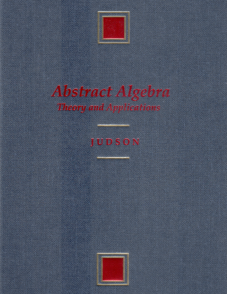
\includepdf[noautoscale=false]{external/original-front-cover-aata.pdf}%
\frontmatter
%% begin: half-title
\thispagestyle{empty}
{\titlepagefont\centering
\vspace*{0.28\textheight}
{\Huge PreTeXt Sample Book}\\[2\baselineskip]
{\LARGE Abstract Algebra (SAMPLE ONLY)}\\
}
\clearpage
%% end:   half-title
%% begin: title page
%% Inspired by Peter Wilson's "titleDB" in "titlepages" CTAN package
\thispagestyle{empty}
{\titlepagefont\centering
\vspace*{0.14\textheight}
%% Target for xref to top-level element is ToC
\addtocontents{toc}{\protect\hypertarget{sample-book}{}}
{\Huge PreTeXt Sample Book}\\[\baselineskip]
{\LARGE Abstract Algebra (SAMPLE ONLY)}\\[3\baselineskip]
{\Large Thomas W. Judson}\\[0.5\baselineskip]
{\Large Stephen F. Austin State University}\\[3\baselineskip]
{\Large Isaac Newton, Editor}\\[0.5\baselineskip]
{\Large Trinity College}\\[3\baselineskip]
{\Large Sage Exercises for Abstract Algebra}\\[0.5\baselineskip]
{\normalsize Robert A. Beezer}\\[0.25\baselineskip]
University of Puget Sound\\
[3\baselineskip]
{\Large August 4, 2025}\\}
\clearpage
%% end:   title page
%% begin: copyright-page
\thispagestyle{empty}
\hypertarget{front-colophon}{}\noindent
Thomas W. Judson did his undergraduate work in Illinois, his graduate work in Oregon and presently teaches in Texas.%
\par
He likes to ride his bicycle in France, especially in the high Alps and Pyrenees on the roads of the Tour de France.%
\par
\bigskip\noindent\textbf{About Robert A. Beezer}\space\space
Rob Beezer designed, wrote, and tested the Sage exercises as a contribution to this open source project.%
\par
He also likes to ride his bicycle, and once rode with Tom Judson in the high Alps, in addition to some hiking there, up above the passes the cyclists ride.%
\par
\vspace*{\stretch{2}}
\par\noindent
\textbf{Cover Design}:\ \ Covers 4 U\\
\textbf{Production Editor}:\ \ Vilma Mesa
\par\vspace*{\stretch{2}}
\noindent{\bfseries Edition}: Annual Edition 2015\par\medskip
\noindent{\bfseries Website}: \href{http://abstract.pugetsound.edu}{\nolinkurl{abstract.pugetsound.edu}}\par\medskip
\noindent{\bfseries Website}: \href{http://abstract.pugetsound.edu}{Some text to test bug report}\footnote{\nolinkurl{abstract.pugetsound.edu}\label{frontmatter-1-9-2}}\par\medskip
\noindent\textcopyright{}1997\textendash{}2015\quad{}Thomas W. Judson, Robert A. Beezer\\[0.5\baselineskip]
Permission is granted to copy, distribute and\slash{}or modify this document under the terms of the GNU Free Documentation License, Version 1.2 or any later version published by the Free Software Foundation; with no Invariant Sections, no Front-Cover Texts, and no Back-Cover Texts.  A copy of the license is included in the appendix entitled ``GNU Free Documentation License.''  All trademarks\texttrademark{} are the registered\textregistered{} marks of their respective owners. An \href{https://example.com}{external link}\footnote{\nolinkurl{example.com}\label{frontmatter-1-10-4-5}} is included\footnote{A second footnote, as well.\label{frontmatter-1-10-4-6}} to test its footnote.\par\medskip
\vspace*{\stretch{1}}
%% Funding/Support statement:\par\medskip
\noindent{}This work has received assistance from numerous volunteer contributors.%
\par
\vspace*{\stretch{1}}
\null\clearpage
%% end:   copyright-page
%% begin: dedication-page
\cleardoublepage
\thispagestyle{empty}
\vspace*{\stretch{1}}
\begin{center}\Large%
To students of algebra everywhere\\
 they are the reason%
\end{center}
\begin{center}\Large%
And to those who teach them%
\end{center}
\vspace*{\stretch{2}}
\clearpage
%% end:   dedication-page
%
%
\typeout{************************************************}
\typeout{Acknowledgements  Acknowledgements}
\typeout{************************************************}
%
\begin{acknowledgement}{Acknowledgements}{Acknowledgements}{}{Acknowledgements}{}{}{acknowledgement}
I would like to acknowledge the following reviewers for their helpful comments and suggestions.%
\begin{itemize}[label=\textbullet]
\item{}David Anderson, University of Tennessee, Knoxville%
\item{}Robert Beezer, University of Puget Sound%
\item{}Myron Hood, California Polytechnic State University%
\item{}Herbert Kasube, Bradley University%
\item{}John Kurtzke, University of Portland%
\item{}Inessa Levi, University of Louisville%
\item{}Geoffrey Mason, University of California, Santa Cruz%
\item{}Bruce Mericle, Mankato State University%
\item{}Kimmo Rosenthal, Union College%
\item{}Mark Teply, University of Wisconsin%
\end{itemize}
%
\par
I would also like to thank Steve Quigley, Marnie Pommett, Cathie Griffin, Kelle Karshick, and the rest of the staff at PWS Publishing for their guidance throughout this project. It has been a pleasure to work with them.%
\par
Robert Beezer encouraged me to make \emph{Abstract Algebra: Theory and Applications} available as an open source textbook, a decision that I have never regretted.  With his assistance, the book has been rewritten in PreTeXt (\href{https://pretextbook.org}{\nolinkurl{pretextbook.org}}), making it possible to quickly output print, web, PDF versions and more from the same source.  The open source version of this book has received support from the National Science Foundation (Award \#DUE-1020957).%
\end{acknowledgement}
%
%
\typeout{************************************************}
\typeout{Preface  Preface}
\typeout{************************************************}
%
\begin{preface}{Preface}{Preface}{}{Preface}{}{}{preface}
This text is intended for a one or two-semester undergraduate course in  abstract algebra. Traditionally, these courses have covered the theoretical aspects of groups, rings, and fields.  However, with the development of computing in the last several decades, applications that involve abstract algebra and discrete mathematics have become increasingly important, and many science, engineering, and computer science students are now electing to minor in mathematics. Though theory still occupies a central role in the subject of abstract algebra and no student should go through such a course without a good notion of what a proof is, the importance of applications such as coding theory and cryptography has grown significantly.%
\par
Until recently most abstract algebra texts included few if any applications. However, one of the major problems in teaching an abstract algebra course is that for many students it is their first encounter with an environment that requires them to do rigorous proofs. Such students often find it hard to see the use of learning to prove theorems and propositions; applied examples help the instructor provide motivation.%
\par
This text contains more material than can possibly be covered in a single semester.  Certainly there is adequate material for a two-semester course, and perhaps more; however, for a one-semester course it would be quite easy to omit selected chapters and still have a useful text.  The order of presentation of topics is standard: groups, then rings, and finally fields. Emphasis can be placed either on theory or on applications. A typical one-semester course might cover groups and rings while briefly touching on field theory, using Chapters~1 through 6, 9, 10, 11, 13 (the first part), 16, 17, 18 (the first part), 20, and 21. Parts of these chapters could be deleted and applications substituted according to the interests of the students and the instructor. A two-semester course emphasizing theory might cover Chapters~1 through 6, 9, 10, 11, 13 through 18, 20, 21, 22 (the first part), and 23. On the other hand, if applications are to be emphasized, the course might cover Chapters 1 through 14, and 16 through 22. In an applied course, some of the more theoretical results could be assumed or omitted. A chapter dependency chart appears below. (A broken line indicates a partial dependency.)  See the \hyperlink{sample-book}{Table of Contents} for more.%
\par
This real text has been used as the basis of a sample book for testing PreTeXt.  So it is slowly migrating away from what the real book looks like and should not be construed as representative.  For example, we have reduced the book to four chapters.%
\begin{image}{0}{1}{0}{}%
\resizebox{\linewidth}{!}{%
\begin{tikzpicture}[scale=0.8]

\draw (3.5,0) rectangle (6.5,1);
\node at (5,0.5) {Chapter 23};

\draw (3.5,1.5) rectangle (6.5,2.5);
\node at (5,2) {Chapter 22};

\draw (3.5,3) rectangle (6.5,4);
\node at (5,3.5) {Chapter 21};

\draw (0,4.5) rectangle (3,5.5);
\node at (1.5,5) {Chapter 18};

\draw (3.5,4.5) rectangle (6.5,5.5);
\node at (5,5) {Chapter 20};

\draw (7,4.5) rectangle (10,5.5);
\node at (8.5,5) {Chapter 19};

\draw (3.5,6) rectangle (6.5,7);
\node at (5,6.5) {Chapter 17};

\draw (10.5,6) rectangle (13.5,7);
\node at (12,6.5) {Chapter 15};

\draw (0,7.5) rectangle (3,8.5);
\node at (1.5,8) {Chapter 13};

\draw (3.5,7.5) rectangle (6.5,8.5);
\node at (5,8) {Chapter 16};

\draw (7,7.5) rectangle (10,8.5);
\node at (8.5,8) {Chapter 12};

\draw (10.5,7.5) rectangle (13.5,8.5);
\node at (12,8) {Chapter 14};

\draw (3.5,9) rectangle (6.5,10);
\node at (5,9.5) {Chapter 11};

\draw (3.5,10.5) rectangle (6.5,11.5);
\node at (5,11) {Chapter 10};

\draw (0,12) rectangle (3,13);
\node at (1.5,12.5) {Chapter 8};

\draw (3.5,12) rectangle (6.5,13);
\node at (5,12.5) {Chapter 9};

\draw (7,12) rectangle (10,13);
\node at (8.5,12.5) {Chapter 7};

\draw (3.5,13.5) rectangle (6.5,14.5);
\node at (5,14) {Chapters 1--6};

\draw (5,1) -- (5,1.5) (5,2.5) -- (5,3)  (5,4) -- (5,4.5)  (5,5.5) -- (5,6)  (5,7) -- (5,7.5)  (5,8.5) -- (5,9)  (5,10) -- (5,10.5)  (5,11.5) -- (5,12)  (5,13) -- (5,13.5);

\draw [dashed] (6.5,0.5) -- (12,0.5) -- (12,6);

\draw (12,7) -- (12,7.5) (12,8.5) -- (12,9.5) -- (6.5,9.5) (8.5,8.5) -- (8.5,9.5);

\draw (8.5,5.5) -- (8.5,6.5) -- (6.5,6.5);

\draw (8.5,13) -- (8.5,14) -- (6.5,14);

\draw [dashed] (3.5,0.5) -- (-0.5,0.5) -- (-0.5,8) -- (0,8);

\draw [dashed] (3.5,2) -- (-1,2) -- (-1,12.5) -- (0,12.5);

\draw (1.5,5.5) -- (1.5,6.5) -- (3.5,6.5);

\draw (1.5,8.5) -- (1.5,9.5) -- (3.5,9.5);

\draw (1.5,13) -- (1.5,14) -- (3.5,14);

\end{tikzpicture}%
}%
\end{image}%
Though there are no specific prerequisites for a course in abstract algebra, students who have had other higher-level courses in mathematics will generally be more prepared than those who have not, because they will possess a bit more mathematical sophistication. Occasionally, we shall assume some basic linear algebra; that is, we shall take for granted an elementary knowledge of matrices and determinants. This should present no great problem, since most students taking a course in abstract algebra have been introduced to matrices and determinants elsewhere in their career, if they have not already taken a sophomore or junior-level course in linear algebra.%
\par
Exercise sections are the heart of any mathematics text. An exercise set appears at the end of each chapter. The nature of the exercises ranges over several categories; computational,  conceptual, and theoretical problems are included. A section presenting hints and solutions to many of the exercises appears at the end of the text. Often in the solutions a proof is only sketched, and it is up to the student to provide the details. The exercises range in difficulty from very easy to very challenging. Many of the more substantial problems require careful thought, so the student should not be discouraged if the 	solution is not forthcoming after a few minutes of work.%
\par
There are additional exercises or computer projects at the ends of many of the chapters. The computer projects usually require a knowledge of programming. All of these exercises and projects are more substantial in nature and allow the exploration of new results and theory.%
\par
Sage (\href{http://sagemath.org}{\nolinkurl{sagemath.org}}) is a free, open source, software system for advanced mathematics, which is ideal for assisting with a study of abstract algebra. Sage can be used either on your own computer, a local server, or on SageMathCloud (\href{https://cloud.sagemath.com}{\nolinkurl{cloud.sagemath.com}}). Robert Beezer has written a comprehensive introduction to Sage and a selection of relevant exercises that appear at the end of each chapter, including live Sage cells in the web version of the book.%
\nopagebreak\par%
\hfill\begin{tabular}[t]{l@{}}
Thomas W. Judson\\
Nacogdoches, Texas 2015
\end{tabular}\\\par
\end{preface}
%
%
\typeout{************************************************}
\typeout{Preface  Contributors to the 4\(^\mathrm{th}\) Edition}
\typeout{************************************************}
%
\begin{preface}{Preface}{Contributors to the 4\(^\mathrm{th}\) Edition}{}{Contributors to the 4\(^\mathrm{th}\) Edition}{}{}{contributors}
Many individuals have made this book possible.  We will try to thank a few of them here, and hope we have not forgotten anybody really important.%
\begin{multicols}{2}
\hypertarget{tjudson}{}%
\contributor{%
\contributorname{Thomas Judson}%
\contributorinfo{Department of Mathematics and Statistics\\
Stephen F. Austin State University\\
\mono{\href{mailto:judsontw@sfasu.edu}{\nolinkurl{judsontw@sfasu.edu}}}}%
}%
\hypertarget{dfarmer}{}%
\contributor{%
\contributorname{David Farmer}%
\contributorinfo{American Institute of Mathematics\\
\mono{\href{mailto:farmer@aimath.org}{\nolinkurl{farmer@aimath.org}}}}%
}%
\hypertarget{contributors-3-3}{}%
\contributor{%
\contributorname{Robert Beezer}%
\contributorinfo{Department of Mathematics and Computer Science\\
University of Puget Sound\\
Tacoma, Washington, USA\\
\mono{\href{mailto:beezer@pugetsound.edu}{\nolinkurl{beezer@pugetsound.edu}}}}%
}%
\hypertarget{contributors-3-4}{}%
\contributor{%
\contributorname{Alex Jordan}%
\contributorinfo{Department of Mathematics\\
Portland Community College\\
Portland, OR\\
\mono{\href{mailto:alex.jordan@pcc.edu}{\nolinkurl{alex.jordan@pcc.edu}}}}%
}%
\hypertarget{contributors-3-5}{}%
\contributor{%
\contributorname{Thomas Judson}%
\contributorinfo{Department of Mathematics and Statistics\\
Stephen F. Austin State University\\
\mono{\href{mailto:judsontw@sfasu.edu}{\nolinkurl{judsontw@sfasu.edu}}}}%
}%
\hypertarget{contributors-3-6}{}%
\contributor{%
\contributorname{David Farmer}%
\contributorinfo{American Institute of Mathematics\\
\mono{\href{mailto:farmer@aimath.org}{\nolinkurl{farmer@aimath.org}}}}%
}%
\hypertarget{contributors-3-7}{}%
\contributor{%
\contributorname{Robert Beezer}%
\contributorinfo{Department of Mathematics and Computer Science\\
University of Puget Sound\\
Tacoma, Washington, USA\\
\mono{\href{mailto:beezer@pugetsound.edu}{\nolinkurl{beezer@pugetsound.edu}}}}%
}%
\hypertarget{ajordan}{}%
\contributor{%
\contributorname{Alex Jordan}%
\contributorinfo{Department of Mathematics\\
Portland Community College\\
Portland, OR\\
\mono{\href{mailto:alex.jordan@pcc.edu}{\nolinkurl{alex.jordan@pcc.edu}}}}%
}%
\hypertarget{contributors-3-9}{}%
\contributor{%
\contributorname{Thomas Judson}%
\contributorinfo{Department of Mathematics and Statistics\\
Stephen F. Austin State University\\
\mono{\href{mailto:judsontw@sfasu.edu}{\nolinkurl{judsontw@sfasu.edu}}}}%
}%
\hypertarget{contributors-3-10}{}%
\contributor{%
\contributorname{David Farmer}%
\contributorinfo{American Institute of Mathematics\\
\mono{\href{mailto:farmer@aimath.org}{\nolinkurl{farmer@aimath.org}}}}%
}%
\hypertarget{contributors-3-11}{}%
\contributor{%
\contributorname{Robert Beezer}%
\contributorinfo{Department of Mathematics and Computer Science\\
University of Puget Sound\\
Tacoma, Washington, USA\\
\mono{\href{mailto:beezer@pugetsound.edu}{\nolinkurl{beezer@pugetsound.edu}}}}%
}%
\hypertarget{contributors-3-12}{}%
\contributor{%
\contributorname{Alex Jordan}%
\contributorinfo{Department of Mathematics\\
Portland Community College\\
Portland, OR\\
\mono{\href{mailto:alex.jordan@pcc.edu}{\nolinkurl{alex.jordan@pcc.edu}}}}%
}%
\hypertarget{contributors-3-13}{}%
\contributor{%
\contributorname{Thomas Judson}%
\contributorinfo{Department of Mathematics and Statistics\\
Stephen F. Austin State University\\
\mono{\href{mailto:judsontw@sfasu.edu}{\nolinkurl{judsontw@sfasu.edu}}}}%
}%
\hypertarget{contributors-3-14}{}%
\contributor{%
\contributorname{David Farmer}%
\contributorinfo{American Institute of Mathematics\\
\mono{\href{mailto:farmer@aimath.org}{\nolinkurl{farmer@aimath.org}}}}%
}%
\hypertarget{rbeezer}{}%
\contributor{%
\contributorname{Robert Beezer}%
\contributorinfo{Department of Mathematics and Computer Science\\
University of Puget Sound\\
Tacoma, Washington, USA\\
\mono{\href{mailto:beezer@pugetsound.edu}{\nolinkurl{beezer@pugetsound.edu}}}}%
}%
\hypertarget{contributors-3-16}{}%
\contributor{%
\contributorname{Alex Jordan}%
\contributorinfo{Department of Mathematics\\
Portland Community College\\
Portland, OR\\
\mono{\href{mailto:alex.jordan@pcc.edu}{\nolinkurl{alex.jordan@pcc.edu}}}}%
}%
\hypertarget{contributors-3-17}{}%
\contributor{%
\contributorname{Thomas Judson}%
\contributorinfo{Department of Mathematics and Statistics\\
Stephen F. Austin State University\\
\mono{\href{mailto:judsontw@sfasu.edu}{\nolinkurl{judsontw@sfasu.edu}}}}%
}%
\hypertarget{contributors-3-18}{}%
\contributor{%
\contributorname{David Farmer}%
\contributorinfo{American Institute of Mathematics\\
\mono{\href{mailto:farmer@aimath.org}{\nolinkurl{farmer@aimath.org}}}}%
}%
\hypertarget{contributors-3-19}{}%
\contributor{%
\contributorname{Robert Beezer}%
\contributorinfo{Department of Mathematics and Computer Science\\
University of Puget Sound\\
Tacoma, Washington, USA\\
\mono{\href{mailto:beezer@pugetsound.edu}{\nolinkurl{beezer@pugetsound.edu}}}}%
}%
\hypertarget{contributors-3-20}{}%
\contributor{%
\contributorname{Alex Jordan}%
\contributorinfo{Department of Mathematics\\
Portland Community College\\
Portland, OR\\
\mono{\href{mailto:alex.jordan@pcc.edu}{\nolinkurl{alex.jordan@pcc.edu}}}}%
}%
\end{multicols}
That's it.  Thanks everybody.%
\end{preface}
%% begin: table of contents
%% Adjust Table of Contents
\setcounter{tocdepth}{1}
\renewcommand*\contentsname{Contents}
\tableofcontents
%% end:   table of contents
\mainmatter
%
%
\typeout{************************************************}
\typeout{Chapter 1 Preliminaries}
\typeout{************************************************}
%
\begin{chapterptx}{Chapter}{Preliminaries}{}{Preliminaries}{}{}{sets}
\renewcommand*{\chaptername}{Chapter}
\begin{introduction}{}%
A certain amount of mathematical maturity is necessary to find and study applications of abstract algebra.  A basic knowledge of set theory, mathematical induction, equivalence relations, and matrices is a must.  Even more important is the ability to read and understand mathematical proofs.  In this chapter we will outline the background needed for a course in abstract algebra.%
\par
It helps when testing to know when this sample document was generated: August 4, 2025, 06:36:33 (-06:00).%
\end{introduction}%
%
%
\typeout{************************************************}
\typeout{Section 1.1 A Short Note on Proofs}
\typeout{************************************************}
%
\begin{sectionptx}{Section}{A Short Note on Proofs}{}{A Short Note on Proofs}{}{}{section-note-on-proofs}
\begin{introduction}{}%
Abstract mathematics is different from other sciences. In laboratory sciences such as chemistry and physics, scientists perform experiments to discover new principles and verify theories.  Although mathematics is often motivated by physical experimentation or by computer simulations, it is made rigorous through the use of logical arguments.  In studying abstract mathematics, we take what is called an  axiomatic approach; that is, we take a collection of objects \(\mathcal S\) and assume some rules about their structure.  These rules are called \terminology{axioms}.  Using the axioms for \(\mathcal S\), we wish to derive other information about \(\mathcal S\) by using logical arguments.  We require that our axioms be consistent; that is, they should not contradict one another.  We also demand that there not be too many axioms. If a system of axioms is too restrictive,  there will be few examples of the mathematical structure.%
\par
A \terminology{statement} in logic or mathematics is an assertion that is either true or false.  Consider the following examples:%
\begin{itemize}[label=\textbullet]
\item{}\(3 + 56 - 13 + 8/2 \).%
\item{}All cats are black.%
\item{}\(2 + 3 = 5\).%
\item{}\(2x = 6\) exactly when \(x = 4\).%
\item{}If \(ax^2 + bx + c = 0\) and \(a \neq 0\), then%
\begin{equation*}
x = \frac{-b \pm \sqrt{b^2 - 4ac}}{2a}\text{.}
\end{equation*}
%
\item{}\(x^3 - 4x^2 + 5 x - 6\).%
\end{itemize}
All but the first and last examples are statements, and must be either true or false.%
\par
A \terminology{mathematical proof} is nothing more than a convincing argument about the accuracy  of a statement. Such an argument should contain enough detail to convince the audience; for instance, we can see that the statement ``\(2x = 6\) exactly when \(x = 4\)'' is false by evaluating \(2 \cdot 4\) and noting that \(6 \neq 8\), an argument that would satisfy anyone. Of course, audiences may vary widely: proofs can be addressed to another student, to a professor, or to the reader of a text.  If more detail than  needed is presented in the proof, then the  explanation will be either long-winded or poorly written.  If too much detail is omitted, then the proof may  not be convincing.  Again it is important to keep the audience in mind.  High school students require much more detail than do graduate students.  A good rule of thumb for an argument in an introductory abstract algebra course is that it should be written to convince one's peers, whether those peers be other students or other readers of the text.%
\par
Let us examine different types of statements.  A statement could be as simple as ``\(10/5 = 2\);'' however, mathematicians are usually interested in more complex statements such as ``If \(p\), then \(q\),'' where \(p\) and \(q\) are both statements.  If certain statements are known or assumed to be true, we wish to know what we can say about other statements.  Here \(p\) is called the \terminology{hypothesis} and \(q\) is known as the \terminology{conclusion}.  Consider the following statement: If \(ax^2 + bx + c = 0\) and \(a \neq 0\), then%
\begin{equation*}
x = \frac{-b \pm \sqrt{b^2 - 4ac}}{2a}\text{.}
\end{equation*}
The hypothesis is \(ax^2 + bx + c = 0\) and \(a \neq 0\); the conclusion is%
\begin{equation*}
x = \frac{-b \pm \sqrt{b^2 - 4ac}}{2a}\text{.}
\end{equation*}
Notice that the  statement says nothing about whether or not the hypothesis is true. However, if this entire statement is true and we can show that \(ax^2 + bx + c = 0\) with \(a \neq 0\) is true, then the conclusion \emph{must} be true.  A proof of this statement might simply be a series of equations:%
\begin{align*}
ax^2 + bx + c & =  0\\
x^2 + \frac{b}{a}x & =  - \frac{c}{a}\\
x^2 + \frac{b}{a}x + \left( \frac{b}{2a} \right)^2 & =  \left( \frac{b}{2a} \right)^2 - \frac{c}{a}\\
\left(x + \frac{b}{2a} \right)^2 & =  \frac{b^2 - 4ac}{4a^2}\\
x + \frac{b}{2a}  & =  \frac{ \pm \sqrt{ b^2 -4ac}}{2a}\\
x & =  \frac{-b \pm \sqrt{b^2 - 4ac}}{2a}\text{.}
\end{align*}
%
\par
If we can prove a statement true, then that statement is called a \terminology{proposition}.  A proposition of major importance is called a \terminology{theorem}.  Sometimes instead of proving a theorem or proposition all at once, we break the proof down into modules; that is, we prove several supporting propositions, which are called \terminology{lemmas}, and use the results of these propositions to prove the main result. If we can prove a proposition or a theorem, we will often, with very little effort, be able to derive other related propositions called \terminology{corollaries}.%
\end{introduction}%
%
%
\typeout{************************************************}
\typeout{Subsection 1.1.1 Some Cautions and Suggestions}
\typeout{************************************************}
%
\begin{subsectionptx}{Subsection}{Some Cautions and Suggestions}{}{Some Cautions and Suggestions}{}{}{section-note-on-proofs-3}
There are several different strategies for proving propositions.  In addition to using different methods of proof, students often make some common mistakes when they are first learning how to prove theorems. To aid students who are studying abstract mathematics for the first time, we list here some of the difficulties that they may encounter and some of the strategies of proof available to them. It is a good idea to keep referring back to this list as a reminder. (Other techniques of proof will become apparent throughout this chapter and the remainder of the text.)%
\begin{itemize}[label=\textbullet]
\item{}A theorem cannot be proved by example; however, the standard way to show that a statement is not a theorem is to provide a counterexample.%
\item{}Quantifiers are important. Words and phrases such as \emph{only}, \emph{for all}, \emph{for every}, and \emph{for some} possess different meanings.%
\item{}Never assume any hypothesis that is not explicitly stated in the theorem.  \emph{You cannot take things for granted.}%
\item{}Suppose you wish to show that an object \emph{exists} and is \emph{unique}.  First show that there actually is such an object.  To show that it is unique, assume that there are two such objects, say \(r\) and \(s\), and then show that \(r = s\).%
\item{}Sometimes it is easier to prove the contrapositive of a statement.  Proving the statement ``If \(p\), then \(q\)'' is exactly the same as proving the statement ``If not \(q\), then not \(p\).''%
\item{}Although it is usually better to find a direct proof of a theorem, this task  can sometimes be difficult. It may be easier to assume that the theorem that you are trying to prove is false, and to hope that in the course of your argument you are forced to make some statement that cannot possibly be true.%
\end{itemize}
%
\par
Remember that one of the main objectives of higher mathematics is proving theorems. Theorems are tools that make new and productive applications of mathematics possible.  We use examples to give insight  into existing theorems and to foster intuitions as to what new theorems might be true.  Applications, examples, and proofs are tightly interconnected\textemdash{}much more so than they may seem at first appearance.%
\end{subsectionptx}
\end{sectionptx}
%
%
\typeout{************************************************}
\typeout{Section 1.2 Sets and Equivalence Relations}
\typeout{************************************************}
%
\begin{sectionptx}{Section}{Sets and Equivalence Relations}{}{Sets and Equivalence Relations}{}{}{section-sets-and-equivalence-relations}
%
%
\typeout{************************************************}
\typeout{Subsection 1.2.1 Set Theory}
\typeout{************************************************}
%
\begin{subsectionptx}{Subsection}{Set Theory}{}{Set Theory}{}{}{section-sets-and-equivalence-relations-2}
A \terminology{set} is a well-defined collection of objects; that is, it is defined in such a manner that we can determine for any given object \(x\) whether or not \(x\) belongs to the set.  The objects that belong to a set are called its \terminology{elements} or \terminology{members}. We will denote sets by capital letters, such as \(A\) or \(X\); if \(a\) is an element of the set \(A\), we write \(a \in A\). \label{section-sets-and-equivalence-relations-2-2-11}%
\par
A set is usually specified either by listing all of its elements inside a pair of braces or by stating the property that determines whether or not an object \(x\) belongs to the set. We might write%
\begin{equation*}
X = \{ x_1, x_2, \ldots, x_n \}
\end{equation*}
for a set containing elements \(x_1, x_2, \ldots, x_n\) or%
\begin{equation*}
X = \{ x :x \text{ satisfies }{\mathcal P}\}
\end{equation*}
if each \(x\) in \(X\) satisfies a certain property \({\mathcal P}\).  For example, if \(E\) is the set of even positive integers, we can describe \(E\) by writing either%
\begin{equation*}
E = \{2, 4, 6, \ldots \} \quad \text{or} \quad E = \{ x : x \text{ is an even integer and } x \gt 0 \}\text{.}
\end{equation*}
We write \(2 \in E\) when we want to say that 2 is in the set \(E\), and \(-3 \notin E\) to say that \(-3\) is not in the set \(E\).%
\par
Some of the more important sets that we will consider are the following:%
\begin{align*}
{\mathbb N} &= \{n: n \text{ is a natural number}\}  = \{1, 2, 3, \ldots \}\\
{\mathbb Z} &= \{n : n \text{ is an integer} \} = \{\ldots, -1, 0, 1,  2, \ldots \}\\
{\mathbb Q} &= \{r : r \text{ is a rational number}\} = \{p/q : p, q \in {\mathbb Z} \text{ where } q \neq 0\}\\
{\mathbb R} &= \{ x : x \text{ is a real number} \}\\
{\mathbb C} &= \{z : z \text{ is a complex number}\}\text{.}
\end{align*}
\label{section-sets-and-equivalence-relations-2-4-2}\label{section-sets-and-equivalence-relations-2-4-3}\label{section-sets-and-equivalence-relations-2-4-4}\label{section-sets-and-equivalence-relations-2-4-5}\label{section-sets-and-equivalence-relations-2-4-6}%
\par
We can find various relations between sets as well as perform operations on sets.  A set \(A\) is a \terminology{subset} of \(B\), written \(A \subset B\) or \(B \supset A\), if every element of \(A\) is also an element of \(B\).  \label{section-sets-and-equivalence-relations-2-5-8} For example,%
\begin{equation*}
\{4,5,8\} \subset \{2, 3, 4, 5, 6, 7, 8, 9 \}
\end{equation*}
and%
\begin{equation*}
{\mathbb N} \subset {\mathbb Z} \subset {\mathbb Q} \subset {\mathbb R} \subset {\mathbb C}\text{.}
\end{equation*}
Trivially, every set is a subset of itself.  A set \(B\) is a \terminology{proper subset} of a set \(A\) if \(B \subset A\) but \(B \neq A\). If \(A\) is not a subset of \(B\), we write \(A \notsubset B\); for example, \(\{4, 7, 9\} \notsubset \{2, 4, 5,  8, 9 \}\).  Two sets are \terminology{equal}, written \(A = B\), if we can show that \(A \subset B\) and \(B \subset A\).%
\par
It is convenient to have a set with no elements in it.  This set is called the \terminology{empty set} and is denoted by \(\emptyset\).  Note that the empty set is a subset of every set. \label{section-sets-and-equivalence-relations-2-6-3}%
\par
To construct new sets out of old sets, we can perform certain operations: the \terminology{union} \(A \cup B\) of two sets \(A\) and \(B\) is defined as%
\begin{equation*}
A \cup B = \{x : x \in A \text{ or } x \in B \}
\end{equation*}
and the \terminology{intersection} of \(A\) and \(B\)  is defined by%
\begin{equation*}
A \cap B = \{x :  x \in A \text{ and } x \in B \}\text{.}
\end{equation*}
\label{section-sets-and-equivalence-relations-2-7-10}\label{section-sets-and-equivalence-relations-2-7-11} If \(A = \{1, 3, 5\}\) and \(B = \{ 1, 2, 3, 9 \}\), then%
\begin{equation*}
A \cup B = \{1, 2, 3, 5, 9 \} \quad \text{and} \quad A \cap B = \{ 1, 3 \}\text{.}
\end{equation*}
We can consider the union and the intersection of more than two sets.  In this case we write%
\begin{equation*}
\bigcup_{i = 1}^{n} A_{i} = A_{1} \cup \ldots \cup A_n
\end{equation*}
and%
\begin{equation*}
\bigcap_{i = 1}^{n} A_{i} = A_{1} \cap \ldots \cap A_n
\end{equation*}
for the union and intersection, respectively, of the sets \(A_1, \ldots, A_n\).%
\par
When two sets have no elements in common, they are said to be \terminology{disjoint}; for example, if \(E\) is the set of even integers and \(O\) is the set of odd integers, then \(E\) and \(O\) are disjoint.  Two sets \(A\) and \(B\) are disjoint exactly when \(A \cap B = \emptyset\).%
\par
Sometimes we will work within one fixed set \(U\), called the \terminology{universal set}.  For any set \(A \subset U\), we define the \terminology{complement} of \(A\), denoted by \(A'\), to be the set \label{section-sets-and-equivalence-relations-2-9-7}%
\begin{equation*}
A' = \{ x : x \in U \text{ and } x \notin A \}\text{.}
\end{equation*}
%
\par
We define the \terminology{difference} of two sets \(A\) and \(B\) to be \label{section-sets-and-equivalence-relations-2-10-4}%
\begin{equation*}
A \setminus B = A \cap B'  = \{ x : x \in A \text{ and } x \notin B \}\text{.}
\end{equation*}
%
\begin{example}{Example}{Set Operations.}{example-sets-operations}%
Let \({\mathbb R}\) be the universal set and suppose that%
\begin{equation*}
A = \{ x \in {\mathbb R} : 0 \lt x \leq 3 \} \quad \text{and} \quad B = \{ x \in {\mathbb R} : 2 \leq x \lt 4 \}\text{.}
\end{equation*}
Then%
\begin{align*}
A \cap B & =  \{ x \in {\mathbb R} : 2 \leq x \leq 3 \}\\
A \cup B & =  \{ x \in {\mathbb R} : 0 \lt x \lt 4 \}\\
A \setminus B & =  \{ x \in {\mathbb R} : 0 \lt x \lt 2  \}\\
A' & =  \{ x \in {\mathbb R} : x \leq 0 \text{ or } x \gt 3 \}\text{.}
\end{align*}
%
\end{example}
\begin{proposition}{Proposition}{}{}{section-sets-and-equivalence-relations-2-12}%
Let \(A\), \(B\), and \(C\) be sets. Then%
\begin{enumerate}
\item{}\(A \cup A = A\), \(A \cap A = A\), and \(A \setminus A = \emptyset\);%
\item{}\(A \cup \emptyset = A\) and \(A \cap \emptyset = \emptyset\);%
\item{}\(A \cup (B \cup C) = (A \cup B) \cup C\) and  \(A \cap (B \cap C) = (A \cap B) \cap C\);%
\item{}\(A \cup B = B \cup A\) and \(A \cap B = B \cap A\);%
\item{}\(A \cup (B \cap C) = (A \cup B) \cap (A \cup C)\);%
\item{}\(A \cap (B \cup C) = (A \cap B) \cup (A \cap C)\).%
\end{enumerate}
%
\end{proposition}
\begin{proof}{Proof}{}{section-sets-and-equivalence-relations-2-12-2}
We will prove (1) and (3) and leave the remaining results to be proven in the exercises.%
\par
(1) Observe that%
\begin{align*}
A \cup A & =  \{ x :  x \in A \text{ or } x \in A \}\\
& =  \{ x : x \in A \}\\
& =  A\\
\intertext{and}
A \cap A & =  \{ x : x \in A \text{ and } x \in A \}\\
& =  \{ x : x \in A  \}\\
& =  A\text{.}
\end{align*}
%
\par
Also, \(A \setminus A = A \cap A' = \emptyset\).%
\par
(3) For sets \(A\), \(B\), and \(C\),%
\begin{align*}
A \cup (B \cup C) & = A \cup \{ x : x \in B \text{ or } x \in C \}\\
& = \{ x : x \in A \text{ or } x \in B, \text{ or } x \in C \}\\
& = \{ x : x \in A \text{ or } x \in B \} \cup C\\
& = (A \cup B) \cup C. 
\end{align*}
%
\par
A similar argument proves that  \(A \cap (B \cap C) = (A \cap B) \cap C\).%
\end{proof}
\begin{theorem}{Theorem}{De Morgan's Laws.}{Augustus De Morgan, 1806\textendash{}1871}{section-sets-and-equivalence-relations-2-13}%
\index{De Morgan's laws!for sets}%
Let \(A\) and \(B\) be sets. Then%
\begin{enumerate}
\item{}\((A \cup B)' = A' \cap B'\);%
\item{}\((A \cap B)' = A' \cup B'\).%
\end{enumerate}
%
\end{theorem}
\begin{proof}{Proof}{}{section-sets-and-equivalence-relations-2-13-5}
(1) We must show that \((A \cup B)' \subset A' \cap B'\) and \((A \cup B)' \supset A' \cap B'\). Let \(x \in (A \cup B)'\).  Then \(x \notin A \cup B\). So \(x\) is neither in \(A\) nor in \(B\), by the definition of the union of sets.  By the definition of the complement, \(x \in A'\) and \(x \in B'\).  Therefore, \(x \in A' \cap B'\) and we have \((A \cup B)' \subset A' \cap B'\).%
\par
To show the reverse inclusion, suppose that \(x \in A' \cap B'\).  Then \(x \in A'\) and \(x \in B'\), and so \(x \notin A\) and \(x \notin B\). Thus \(x \notin A \cup B\) and so \(x \in (A \cup B)'\).  Hence, \((A \cup B)' \supset A' \cap B'\) and so \((A \cup B)' = A' \cap B'\).%
\par
The proof of (2) is left as an exercise.%
\end{proof}
\begin{example}{Example}{Other Relations on Sets.}{example-sets-other-relations}%
Other relations between sets often hold true. For example,%
\begin{equation*}
( A \setminus B) \cap (B \setminus A) = \emptyset\text{.}
\end{equation*}
To see that this is true, observe that%
\begin{align*}
( A \setminus B) \cap (B \setminus A) & = ( A \cap B') \cap (B \cap A')\\
& = A \cap A' \cap B \cap B'\\
& = \emptyset\text{.}
\end{align*}
%
\end{example}
\end{subsectionptx}
%
%
\typeout{************************************************}
\typeout{Subsection 1.2.2 Cartesian Products and Mappings}
\typeout{************************************************}
%
\begin{subsectionptx}{Subsection}{Cartesian Products and Mappings}{}{Cartesian Products and Mappings}{}{}{section-sets-and-equivalence-relations-3}
Given sets \(A\) and \(B\), we can define a new set \(A \times B\), called the \terminology{Cartesian product}  of \(A\) and \(B\), as a set of ordered pairs.  That is, \label{section-sets-and-equivalence-relations-3-2-7}%
\begin{equation*}
A \times B = \{ (a,b) : a \in A \text{ and } b \in B \}\text{.}
\end{equation*}
%
\begin{example}{Example}{Cartesian Products.}{example-sets-cartesian-products}%
If \(A = \{ x, y \}\), \(B = \{ 1, 2, 3 \}\), and \(C = \emptyset\), then \(A \times B\) is the set%
\begin{equation*}
\{ (x, 1), (x, 2), (x, 3), (y, 1), (y, 2), (y, 3) \}
\end{equation*}
and%
\begin{equation*}
A \times C = \emptyset\text{.}
\end{equation*}
%
\end{example}
We define the \terminology{Cartesian product of \(n\) sets} to be%
\begin{equation*}
A_1 \times \cdots \times A_n = \{ (a_1, \ldots, a_n): a_i \in A_i \text{ for } i = 1, \ldots, n \}\text{.}
\end{equation*}
If \(A = A_1 = A_2 = \cdots = A_n\), we often write \(A^n\) for \(A \times \cdots \times A\) (where \(A\) would be written \(n\) times).  \label{section-sets-and-equivalence-relations-3-4-8}For example, the set \({\mathbb R}^3\) consists of all of 3-tuples of real numbers.%
\par
Subsets of \(A \times B\) are called \terminology{relations}.  We will define a  \terminology{mapping}\index{Mapping|see{Function}} or \terminology{function}\index{Function!definition of} \(f \subset A \times B\) from a set \(A\) to a set \(B\) to be the special type of relation where \((a, b) \in f\) if for every element \(a \in A\) there exists a unique element \(b \in B\). Another way of saying this is that for every element in \(A\), \(f\) assigns a unique element in \(B\).  We usually write \(f:A \rightarrow B\) or \(A \stackrel{f}{\rightarrow} B\).  Instead of writing down ordered pairs  \((a,b) \in A \times B\), we write \(f(a) = b\) or \(f : a \mapsto b\).  The set  \(A\) is called the \terminology{domain}\index{Function!domain of} of \(f\) and%
\begin{equation*}
f(A) = \{ f(a) : a \in A \} \subset B
\end{equation*}
is called the \terminology{range}\index{Function!range of} or \terminology{image} of \(f\).  We can think of the elements in the function's domain as input values and the elements in the function's range as output values.%
\begin{figureptx}{Figure}{Mappings and relations}{figure-sets-mappings}{}%
\begin{image}{0}{1}{0}{}%
\resizebox{\linewidth}{!}{%
\begin{tikzpicture}[scale=0.5]
\draw (0,0) ellipse (2 and 3);
\draw (7,0) ellipse (2 and 3);
\draw (0,8) ellipse (2 and 3);
\draw (7,8) ellipse (2 and 3);
\draw [->] (0.5,9.5) -- (6.5,8);
\draw [->] (0.5,8) -- (6.5,6.7);
\draw [->] (0.5,6.5) -- (6.5,6.5);
\draw [->] (0.5,1.5) -- (6.5,1.5);
\draw [->] (0.5,1.3) -- (6.5,0);
\draw [->] (0.5,0) -- (6.5,-1.5);
\draw [->] (0.5,-1.5) -- (6.5,1.3);
\node at (0, 1.5) {1};
\node at (0, 0) {2};
\node at (0, -1.5) {3};
\node at (7, 1.5) {$a$};
\node at (7, 0) {$b$};
\node at (7, -1.5) {$c$};
\node at (0, 9.5) {1};
\node at (0, 8) {2};
\node at (0, 6.5) {3};
\node at (7, 9.5) {$a$};
\node at (7, 8) {$b$};
\node at (7, 6.5) {$c$};
\node at (-1.5,11) {$A$};
\node at (5.5,11) {$B$};
\node at (-1.5,3) {$A$};
\node at (5.5,3) {$B$};
\node at (3.5,3) {$g$};
\node at (3.5,10) {$f$};
\end{tikzpicture}%
}%
\end{image}%
\tcblower
\end{figureptx}%
\begin{example}{Example}{Mappings.}{example-sets-mappings}%
Suppose \(A = \{1, 2, 3 \}\) and \(B = \{a, b, c \}\).  In \hyperref[figure-sets-mappings]{Figure~{\xreffont\ref{figure-sets-mappings}}} we define relations \(f\) and  \(g\) from \(A\) to \(B\).  The relation \(f\) is a mapping, but \(g\) is not because \(1 \in A\) is not assigned to a unique element in \(B\); that is, \(g(1) = a\) and \(g(1) = b\).%
\end{example}
Given a function \(f : A \rightarrow B\), it is often possible to write a list describing what the function does to each specific element in the domain.  However, not all functions can be described in this manner.  For example, the function \(f: {\mathbb R} \rightarrow {\mathbb R}\) that sends each real number to its cube is a mapping that must be described by writing \(f(x) = x^3\) or \(f:x \mapsto x^3\).%
\par
Consider the relation \(f : {\mathbb Q} \rightarrow {\mathbb Z}\) given by \(f(p/q) = p\).  We know that \(1/2 = 2/4\), but is \(f(1/2) = 1\) or 2?  This relation cannot be a mapping because it is not well-defined.  A relation is \terminology{well-defined}\index{Well-defined map} if each element in the domain is assigned to a \emph{unique} element in the range.%
\par
If \(f:A \rightarrow B\) is a map and the image of \(f\) is \(B\), i.e., \(f(A) = B\), then \(f\) is said to be \terminology{onto}\index{Function!onto} or \terminology{surjective}\index{Function!surjective}. In other words, if there exists an \(a \in A\) for each \(b \in B\) such that \(f(a) = b\), then \(f\) is onto. A map is \terminology{one-to-one}\index{Function!one-to-one} or \terminology{injective}\index{Function!injective} if \(a_1 \neq a_2\) implies \(f(a_1) \neq f(a_2)\).  Equivalently, a function is one-to-one if \(f(a_1) = f(a_2)\) implies \(a_1 = a_2\).  A map that is both one-to-one and onto is called \terminology{bijective}\index{Function!bijective}.%
\begin{example}{Example}{One-to-One and Onto Mappings.}{example-sets-one-to-one-onto}%
Let \(f:{\mathbb Z} \rightarrow {\mathbb Q}\) be defined by \(f(n) = n/1\).  Then \(f\) is one-to-one but not onto.  Define \(g : {\mathbb Q} \rightarrow {\mathbb Z}\) by \(g(p/q) = p\) where \(p/q\) is a rational number expressed in its lowest terms with a positive denominator.  The function \(g\) is onto but not one-to-one.%
\end{example}
Given two functions, we can construct a new function by using the range of the first function as the domain of the second function.  Let \(f : A \rightarrow B\) and \(g : B \rightarrow C\) be mappings.  Define a new map, the \terminology{composition}\index{Function!composition of} of \(f\) and \(g\) from \(A\) to \(C\), by \((g \circ f)(x) = g(f(x))\).%
\begin{figureptx}{Figure}{Composition of maps}{figure-sets-composition}{}%
\begin{image}{0}{1}{0}{}%
\resizebox{\linewidth}{!}{%
\begin{tikzpicture}[scale=0.5]
\draw (-6,8) ellipse (2 and 3);
\draw (0,8) ellipse (2 and 3);
\draw (6,8) ellipse (2 and 3);

\node at (-7.5,11) {$A$};
\node at (-1.5,11) {$B$};
\node at (4.5,11) {$C$};
\node at (-6, 9.5) {1};
\node at (-6, 8) {2};
\node at (-6, 6.5) {3};
\node at (0, 9.5) {$a$};
\node at (0, 8) {$b$};
\node at (0, 6.5) {$c$};
\node at (6, 9.5) {$X$};
\node at (6, 8) {$Y$};
\node at (6, 6.5) {$Z$};
\node at (-3,10) {$f$};
\node at (3,10) {$g$};

\draw [->] (0.5,9.5) -- (5.5,6.7);
\draw [->] (0.5,8) -- (5.5,6.5);
\draw [->] (0.5,6.5) -- (5.5,9.5);

\draw [->] (-5.5,9.5) -- (-0.5,8);
\draw [->] (-5.5,8) -- (-0.5,6.5);
\draw [->] (-5.5,6.5) -- (-0.5,9.5);

\draw (-3,0) ellipse (2 and 3);
\draw (3,0) ellipse (2 and 3);

\node at (-5,3) {$A$};
\node at (1.5,3) {$C$};
\node at (-3, 1.5) {1};
\node at (-3, 0) {2};
\node at (-3, -1.5) {3};
\node at (3, 1.5) {$X$};
\node at (3, 0) {$Y$};
\node at (3, -1.5) {$Z$};
\node at (0,2.5) {$g \circ f$};

\draw [->] (-2.5,1.5) -- (2.5,-1.3);
\draw [->] (-2.5,0) -- (2.5,1.5);
\draw [->] (-2.5,-1.5) -- (2.5,-1.5);

\end{tikzpicture}%
}%
\end{image}%
\tcblower
\end{figureptx}%
\begin{example}{Example}{Composition of Mappings.}{example-sets-composition}%
Consider the functions \(f: A \rightarrow B\) and \(g: B \rightarrow C\) that are defined in \hyperref[figure-sets-composition]{Figure~{\xreffont\ref{figure-sets-composition}}} (top).  The composition of these functions, \(g \circ f: A \rightarrow C\), is defined in \hyperref[figure-sets-composition]{Figure~{\xreffont\ref{figure-sets-composition}}} (bottom).%
\end{example}
\begin{example}{Example}{Composition is not Commutative.}{example-sets-composition-noncommute}%
Let \(f(x) = x^2\) and \(g(x) = 2x + 5\). Then%
\begin{equation*}
(f \circ g)(x) = f(g(x)) = (2x + 5)^2 = 4x^2 + 20x + 25
\end{equation*}
and%
\begin{equation*}
(g \circ f)(x) = g(f(x)) = 2x^2 + 5\text{.}
\end{equation*}
In general, order makes a difference; that is, in most cases \(f \circ g \neq g \circ f\).%
\end{example}
\begin{example}{Example}{Some Mappings Commute.}{example-sets-composition-commute}%
Sometimes it is the case that \(f \circ g= g \circ f\).  Let \(f(x) = x^3\) and \(g(x) = \sqrt[3]{x}\). Then%
\begin{equation*}
(f \circ g )(x) = f(g(x)) = f( \sqrt[3]{x}\, ) = (\sqrt[3]{x}\, )^3 = x
\end{equation*}
and%
\begin{equation*}
(g \circ f )(x) = g(f(x)) = g( x^3) = \sqrt[3]{ x^3} = x\text{.}
\end{equation*}
%
\end{example}
\begin{example}{Example}{A Linear Map.}{example-sets-linear-map}%
Given a \(2 \times 2\) matrix%
\begin{equation*}
A =
\begin{pmatrix}
a & b \\
c & d
\end{pmatrix}\text{,}
\end{equation*}
we can define a map \(T_A : {\mathbb R}^2 \rightarrow {\mathbb R}^2\) by%
\begin{equation*}
T_A (x,y) = (ax + by, cx +dy)
\end{equation*}
for \((x,y)\) in \({\mathbb R}^2\).  This is actually matrix multiplication; that is,%
\begin{equation*}
\begin{pmatrix}
a & b \\
c & d
\end{pmatrix}
\begin{pmatrix}
x \\ y
\end{pmatrix}
=
\begin{pmatrix}
ax + by \\
cx +dy
\end{pmatrix}\text{.}
\end{equation*}
Maps from \({\mathbb R}^n\) to \({\mathbb R}^m\) given by matrices are called \terminology{linear maps} or \terminology{linear transformations}\index{Linear transformation!definition of}.%
\end{example}
\begin{example}{Example}{A Permutation.}{example-sets-permutation}%
Suppose that \(S = \{ 1,2,3  \}\). Define a map \(\pi :S\rightarrow S\) by%
\begin{equation*}
\pi( 1 )  = 2, \qquad \pi( 2 )  = 1, \qquad \pi( 3 )  = 3\text{.}
\end{equation*}
This is a bijective map.  An alternative way to  write \(\pi\) is%
\begin{equation*}
\begin{pmatrix}
1 & 2 & 3 \\
\pi(1) & \pi(2) & \pi(3)
\end{pmatrix}
=
\begin{pmatrix}
1 & 2 & 3 \\
2 & 1 & 3
\end{pmatrix}\text{.}
\end{equation*}
For any set \(S\), a one-to-one and onto mapping \(\pi : S \rightarrow S\) is called a \terminology{permutation}\index{Permutation!definition of} of \(S\).%
\end{example}
\begin{theorem}{Theorem}{}{}{section-sets-and-equivalence-relations-3-19}%
Let \(f : A \rightarrow B\), \(g : B \rightarrow C\), and \(h : C \rightarrow D\). Then%
\begin{enumerate}
\item{}The composition of mappings is associative; that is, \((h \circ g) \circ f = h \circ (g \circ f)\);%
\item{}If \(f\) and \(g\) are both one-to-one, then the mapping \(g \circ f\) is one-to-one;%
\item{}If \(f\) and \(g\) are both onto, then the mapping \(g \circ f\) is onto;%
\item{}If \(f\) and \(g\) are bijective, then so is \(g \circ f\).%
\end{enumerate}
%
\end{theorem}
\begin{proof}{Proof}{}{section-sets-and-equivalence-relations-3-19-2}
We will prove (1) and (3). Part (2) is left as an exercise.  Part (4) follows directly from (2) and (3).%
\par
(1) We must show that%
\begin{equation*}
h \circ (g \circ f) = (h \circ g) \circ f\text{.}
\end{equation*}
For \(a \in A\) we have%
\begin{align*}
(h \circ (g \circ f))(a) & = h((g \circ f)(a))\\
& = h(g(f(a))) \\
& = (h \circ g)(f(a))\\
& = ((h \circ g) \circ f)(a)\text{.}
\end{align*}
%
\par
(3) Assume that \(f\) and \(g\) are both onto functions. Given \(c \in C\), we must show that there exists an \(a \in A\) such that \((g \circ f)(a) = g(f(a)) = c\). However, since \(g\) is onto, there is an element \(b \in B\) such that \(g(b) = c\). Similarly, there is an \(a \in A\) such that \(f(a) = b\). Accordingly,%
\begin{equation*}
(g \circ f)(a) = g(f(a)) = g(b) = c\text{.}
\end{equation*}
%
\end{proof}
If \(S\) is any set, we will use \(id_S\) or \(id\) to denote the \terminology{identity mapping}\index{Function!identity} from \(S\) to itself.  Define this map by \(id(s) = s\) for all \(s \in S\).  A map \(g: B \rightarrow A\) is an \terminology{inverse mapping} of \(f: A \rightarrow B\) if \(g \circ f = id_A\) and \(f \circ g = id_B\); in other words, the inverse function of a function simply ``undoes'' the function.   A map is said to be \terminology{invertible}\index{Function!invertible} if it has an inverse.  We usually write \(f^{-1}\) for the inverse of \(f\). \label{section-sets-and-equivalence-relations-3-20-19}\label{section-sets-and-equivalence-relations-3-20-20}%
\begin{example}{Example}{An Inverse Function.}{example-sets-inverse-function}%
The function \(f(x) = x^3\) has inverse \(f^{-1}(x) = \sqrt[3]{x}\) by \hyperref[example-sets-composition-commute]{Example~{\xreffont\ref{example-sets-composition-commute}}}.%
\end{example}
\begin{example}{Example}{Exponential and Logarithmic Functions are Inverses.}{example-sets-exponential}%
The natural logarithm and the exponential functions, \(f(x) = \ln x\) and \(f^{-1}(x) = e^x\), are inverses of each other provided that we are careful about choosing domains.  Observe that%
\begin{equation*}
f(f^{-1}(x)) = f(e^x) = \ln e^x = x
\end{equation*}
and%
\begin{equation*}
f^{-1}(f(x)) = f^{-1}(\ln x) = e^{\ln x} = x
\end{equation*}
whenever composition makes sense.%
\end{example}
\begin{example}{Example}{A Matrix Inverse Yields an Inverse of a Linear Map.}{example-sets-inverse-matrix}%
Suppose that%
\begin{equation*}
A =
\begin{pmatrix}
3 & 1 \\
5 & 2
\end{pmatrix}\text{.}
\end{equation*}
Then \(A\) defines a map from \({\mathbb R}^2\) to \({\mathbb R}^2\) by%
\begin{equation*}
T_A (x,y) = (3x +  y, 5x + 2y)\text{.}
\end{equation*}
We can find an inverse map of \(T_A\) by simply inverting the matrix \(A\); that is, \(T_A^{-1} = T_{A^{-1}}\). In this example,%
\begin{equation*}
A^{-1} =
\begin{pmatrix}
2  & -1 \\
-5 &  3
\end{pmatrix}
\end{equation*}
and hence, the inverse map is given by%
\begin{equation*}
T_A^{-1} (x,y) = (2x -  y, -5x + 3y)\text{.}
\end{equation*}
It is easy to check that%
\begin{equation*}
T^{-1}_A \circ T_A (x,y) = T_A \circ T_A^{-1} (x,y) = (x,y)\text{.}
\end{equation*}
Not every map has an inverse.  If we consider the map%
\begin{equation*}
T_B (x,y) = (3x , 0 )
\end{equation*}
given by the matrix%
\begin{equation*}
B =
\begin{pmatrix}
3 & 0 \\
0 & 0
\end{pmatrix}\text{,}
\end{equation*}
then an inverse map would have to be of the form%
\begin{equation*}
T_B^{-1} (x,y) = (ax + by, cx +dy)
\end{equation*}
and%
\begin{equation*}
(x,y) = T \circ T_B^{-1} (x,y) = (3ax + 3by, 0)
\end{equation*}
for all \(x\) and \(y\).  Clearly this is  impossible because \(y\) might not be 0.%
\end{example}
\begin{example}{Example}{An Inverse Permutation.}{example-sets-inverse-permutation}%
Given the permutation%
\begin{equation*}
\pi =
\begin{pmatrix}
1 & 2 & 3 \\
2 & 3 & 1
\end{pmatrix}
\end{equation*}
on \(S = \{ 1,2,3 \}\), it is easy to see that the permutation defined by%
\begin{equation*}
\pi^{-1} =
\begin{pmatrix}
1 & 2 & 3 \\
3 & 1 & 2
\end{pmatrix}
\end{equation*}
is the inverse of \(\pi\).  In fact, any bijective mapping possesses an inverse, as we will see in the next theorem.%
\end{example}
\begin{theorem}{Theorem}{}{}{section-sets-and-equivalence-relations-3-25}%
A mapping is invertible if and only if it is both one-to-one and onto.%
\end{theorem}
\begin{proof}{Proof}{}{section-sets-and-equivalence-relations-3-25-2}
Suppose first that \(f:A \rightarrow B\) is invertible with inverse \(g: B \rightarrow A\). Then \(g \circ f = id_A\) is the identity map; that is, \(g(f(a)) = a\). If \(a_1, a_2 \in A\) with \(f(a_1) = f(a_2)\), then \(a_1 = g(f(a_1)) = g(f(a_2)) = a_2\).  Consequently, \(f\) is one-to-one.  Now suppose that \(b \in B\). To show that \(f\) is onto, it is necessary to find an \(a \in A\) such that \(f(a) = b\), but \(f(g(b)) = b\) with \(g(b) \in A\). Let \(a = g(b)\).%
\par
Conversely, let \(f\) be bijective and let \(b \in B\).  Since \(f\) is onto, there exists an \(a \in A\) such that \(f(a) = b\).  Because \(f\) is one-to-one, \(a\) must be unique. Define \(g\) by letting \(g(b) = a\).  We have now constructed the inverse of \(f\).%
\end{proof}
\end{subsectionptx}
%
%
\typeout{************************************************}
\typeout{Subsection 1.2.3 Equivalence Relations and Partitions}
\typeout{************************************************}
%
\begin{subsectionptx}{Subsection}{Equivalence Relations and Partitions}{}{Equivalence Relations and Partitions}{}{}{section-sets-and-equivalence-relations-4}
A fundamental notion in mathematics is that of equality.  We can generalize equality with equivalence relations and equivalence classes.  An \terminology{equivalence relation}\index{Equivalence relation} on a set \(X\) is a relation \(R \subset X \times X\) such that%
\begin{itemize}[label=\textbullet]
\item{}\((x, x) \in R\) for all \(x \in X\) (\terminology{reflexive property});%
\item{}\((x, y) \in R\) implies \((y, x) \in R\) (\terminology{symmetric property});%
\item{}\((x, y)\) and \((y, z) \in R\) imply \((x, z) \in R\) (\terminology{transitive property}).%
\end{itemize}
%
\par
Given an equivalence relation \(R\)  on a set \(X\), we usually write  \(x \sim y\) instead of \((x, y) \in R\). If the equivalence relation already has an associated notation such as \(=\), \(\equiv\), or \(\cong\), we will use that notation.%
\begin{example}{Example}{Equivalent Fractions.}{example-sets-equivalent-fractions}%
Let \(p\), \(q\), \(r\), and \(s\) be integers, where \(q\) and \(s\) are nonzero.  Define \(p/q \sim r/s\) if \(ps = qr\).  Clearly \(\sim\) is reflexive and symmetric.  To show that it is also transitive, suppose that \(p/q \sim r/s\) and \(r/s \sim t/u\), with \(q\), \(s\), and \(u\) all nonzero.  Then \(ps = qr\) and \(ru = st\). Therefore,%
\begin{equation*}
psu = qru = qst\text{.}
\end{equation*}
Since \(s \neq 0\), \(pu = qt\). Consequently, \(p/q \sim t/u\).%
\end{example}
\begin{example}{Example}{An Equivalence Relation From Derivatives.}{example-sets-equivalent-derivative}%
Suppose that \(f\) and \(g\) are differentiable functions on \({\mathbb R}\).  We can define an equivalence relation on such functions by letting \(f(x) \sim g(x)\) if \(f'(x) = g'(x)\). It is clear that \(\sim\) is both reflexive and symmetric.  To demonstrate transitivity, suppose that \(f(x) \sim g(x)\) and  \(g(x) \sim h(x)\).  From calculus we know that \(f(x) - g(x) = c_1\) and \(g(x)- h(x) = c_2\), where \(c_1\) and \(c_2\) are both constants. Hence,%
\begin{equation*}
f(x) - h(x) = ( f(x) - g(x)) + ( g(x)- h(x))  = c_1 - c_2
\end{equation*}
and \(f'(x) - h'(x) = 0\). Therefore, \(f(x) \sim h(x)\).%
\end{example}
\begin{example}{Example}{Equivalent Circles.}{example-sets-equivalent-circles}%
For \((x_1, y_1 )\) and \((x_2, y_2)\) in \({\mathbb R}^2\), define \((x_1, y_1 ) \sim (x_2, y_2)\) if \(x_1^2 + y_1^2 = x_2^2 + y_2^2\).  Then \(\sim\) is an equivalence relation on \({\mathbb R}^2\).%
\end{example}
\begin{example}{Example}{Equivalent Matrices.}{example-sets-equivalent-matrices}%
Let \(A\) and \(B\) be \(2 \times 2\) matrices with entries in the real numbers. We can define an equivalence relation on the set of \(2 \times 2\) matrices, by saying \(A \sim B\) if there exists an invertible matrix \(P\) such that \(PAP^{-1} = B\).  For example, if%
\begin{equation*}
A =
\begin{pmatrix}
1 & 2 \\
-1 & 1
\end{pmatrix}
\quad \text{and} \quad
B =
\begin{pmatrix}
-18 & 33 \\
-11 & 20
\end{pmatrix}\text{,}
\end{equation*}
then \(A \sim B\) since \(PAP^{-1} = B\) for%
\begin{equation*}
P =
\begin{pmatrix}
2 & 5 \\
1 & 3
\end{pmatrix}\text{.}
\end{equation*}
Let \(I\) be the \(2 \times 2\) identity matrix; that is,%
\begin{equation*}
I =
\begin{pmatrix}
1 & 0 \\
0 & 1
\end{pmatrix}\text{.}
\end{equation*}
Then \(IAI^{-1} = IAI = A\); therefore, the relation is reflexive.  To show symmetry, suppose that \(A \sim B\).  Then there exists an invertible matrix \(P\) such that \(PAP^{-1} = B\).  So%
\begin{equation*}
A = P^{-1} B P = P^{-1} B (P^{-1})^{-1}\text{.}
\end{equation*}
Finally, suppose that \(A \sim B\) and \(B \sim C\).  Then there exist invertible matrices \(P\) and \(Q\) such that \(PAP^{-1} = B\) and  \(QBQ^{-1} = C\).  Since%
\begin{equation*}
C = QBQ^{-1} = QPAP^{-1} Q^{-1} = (QP)A(QP)^{-1}\text{,}
\end{equation*}
the relation is transitive.  Two matrices that are equivalent in this manner are said to be \terminology{similar}\index{Matrix!similar}.%
\end{example}
A \terminology{partition}\index{Partitions} \({\mathcal P}\) of a set \(X\) is a collection of nonempty sets \(X_1, X_2, \ldots\) such that \(X_i \cap X_j = \emptyset\) for \(i  \neq j\) and \(\bigcup_k X_k = X\). Let \(\sim\) be an equivalence relation on a set \(X\) and let \(x \in X\).  Then \([x] = \{ y \in X : y \sim x \}\) is called the \terminology{equivalence class}\index{Equivalence class} of \(x\).  We will see that an equivalence relation gives rise to a partition via equivalence classes.  Also, whenever a partition of a set exists, there is some natural  underlying equivalence relation, as the following theorem demonstrates.%
\begin{theorem}{Theorem}{}{}{section-sets-and-equivalence-relations-4-9}%
Given an equivalence relation \(\sim\) on a set \(X\), the equivalence classes of \(X\) form a partition of \(X\).  Conversely, if \({\mathcal P} = \{ X_i\}\) is a partition of a set \(X\), then there is an equivalence relation on \(X\) with equivalence classes \(X_i\).%
\end{theorem}
\begin{proof}{Proof}{}{section-sets-and-equivalence-relations-4-9-2}
Suppose there exists an equivalence relation \(\sim\) on the set \(X\).  For any \(x \in X\), the reflexive property shows that \(x \in [x]\) and so \([x]\) is nonempty.  Clearly \(X = \bigcup_{x \in X} [x]\).  Now let \(x, y \in X\). We need to show that either \([x] = [y]\) or \([x] \cap [y] = \emptyset\).  Suppose that the intersection of \([x]\) and \([y]\) is not empty and that \(z \in [x] \cap [y]\). Then \(z \sim x\) and \(z \sim y\).  By symmetry and transitivity \(x \sim y\); hence, \([x] \subset [y]\).  Similarly, \([y] \subset [x]\) and so \([x] = [y]\).  Therefore, any two equivalence classes are either disjoint or exactly the same.%
\par
Conversely, suppose that \({\mathcal P} = \{X_i\}\) is a partition of a set \(X\).  Let two elements be equivalent if they are in the same partition.  Clearly, the relation is reflexive.  If \(x\) is in the same partition as \(y\), then \(y\) is in the same partition as \(x\), so \(x \sim y\) implies \(y \sim x\).  Finally, if \(x\) is in the same partition as \(y\) and \(y\) is in the same partition as \(z\), then \(x\) must be in the same partition as \(z\), and transitivity holds.%
\end{proof}
\begin{corollary}{Corollary}{}{}{section-sets-and-equivalence-relations-4-10}%
Two equivalence classes of an equivalence relation are either disjoint or equal.%
\end{corollary}
Let us examine some of the partitions given by the equivalence classes in the last set of examples.%
\begin{example}{Example}{A Partition of Fractions.}{example-sets-fraction-partition}%
In the equivalence relation in \hyperref[example-sets-equivalent-fractions]{Example~{\xreffont\ref{example-sets-equivalent-fractions}}}, two pairs of integers, \((p,q)\) and \((r,s)\), are in the same equivalence class when they reduce to the same fraction in its lowest terms.%
\end{example}
\begin{example}{Example}{A Partition of Functions.}{example-sets-matrix-partition}%
In the equivalence relation in \hyperref[example-sets-equivalent-derivative]{Example~{\xreffont\ref{example-sets-equivalent-derivative}}}, two functions \(f(x)\) and \(g(x)\) are in the same partition when they differ by a constant.%
\end{example}
\begin{example}{Example}{A Partition of Circles.}{example-sets-circle-partition}%
We defined an equivalence class on \({\mathbb R}^2\) by \((x_1, y_1 ) \sim (x_2, y_2)\) if \(x_1^2 + y_1^2 = x_2^2 + y_2^2\).  Two pairs of real numbers are in the same partition when they lie on the same circle about the origin.%
\end{example}
\begin{example}{Example}{A Partition of Integers.}{example-sets-congruent-integers}%
Let \(r\) and \(s\) be two integers and suppose that \(n \in {\mathbb N}\).  We say that \(r\) is \terminology{congruent}\index{Congruence modulo \(n\)} to \(s\) \terminology{modulo} \(n\), or \(r\) is congruent to \(s\) mod \(n\), if \(r - s\) is evenly divisible by \(n\); that is, \(r - s = nk\)  for some \(k \in {\mathbb Z}\).  In this case we write \(r \equiv s \pmod{n}\).  \label{example-sets-congruent-integers-2-18}  For example, \(41 \equiv 17 \pmod{ 8}\) since \(41 - 17=24\) is divisible by 8.  We claim that congruence modulo \(n\) forms an equivalence relation of \({\mathbb Z}\).  Certainly any integer \(r\) is equivalent to itself since \(r - r = 0\) is divisible by \(n\).  We will now show that the relation is symmetric.  If \(r \equiv s \pmod{ n}\), then \(r - s = -(s -r)\) is divisible by \(n\). So \(s - r\) is divisible by \(n\) and \(s \equiv r \pmod{ n}\).  Now suppose that \(r \equiv s \pmod{ n}\) and \(s \equiv t \pmod{ n}\).  Then there exist integers \(k\) and \(l\) such that \(r -s = kn\) and \(s - t = ln\).  To show transitivity, it is necessary to prove that \(r - t\) is divisible by \(n\).  However,%
\begin{equation*}
r - t = r - s + s - t = kn + ln = (k + l)n\text{,}
\end{equation*}
and so \(r - t\) is divisible by \(n\).%
\par
If we consider the equivalence relation established by the integers modulo 3, then%
\begin{align*}
{[0]} & = \{ \ldots, -3, 0, 3, 6, \ldots \}\\
{[1]} & = \{ \ldots, -2, 1, 4, 7, \ldots \}\\
{[2]} & = \{ \ldots, -1, 2, 5, 8, \ldots \}\text{.}
\end{align*}
%
\par
Notice that \([0] \cup [1] \cup [2] = {\mathbb Z}\) and also that the sets are disjoint.  The sets \([0]\), \([1]\), and \([2]\) form a partition of the integers.%
\par
The integers modulo \(n\) are a very important example in the study of abstract algebra and will become quite useful in our investigation of various algebraic structures such as groups and rings.  In our discussion of the integers modulo \(n\) we have actually assumed a result known as the division algorithm, which will be stated and proved in \hyperref[integers]{Chapter~{\xreffont\ref{integers}}}.%
\end{example}
\end{subsectionptx}
\end{sectionptx}
%
%
\typeout{************************************************}
\typeout{Section 1.3 Sage}
\typeout{************************************************}
%
\begin{sectionptx}{Section}{Sage}{}{Sage}{}{}{sets-sage}
\begin{introduction}{}%
Sage is a powerful system for studying and exploring many different areas of mathematics.  In this textbook, you will study a variety of algebraic structures, such as groups, rings and fields.  Sage does an excellent job of implementing many features of these objects as we will see in the chapters ahead.  But here and now, in this initial chapter, we will concentrate on a few general ways of getting the most out of working with Sage.%
\par
You may use Sage several different ways.  It may be used as a command-line program when installed on your own computer.  Or it might be a web application such as the SageMathCloud.  Our writing will assume that you are reading this as a worksheet within the Sage Notebook (a web browser interface), or this is a section of the entire book presented as web pages, and you are employing the Sage Cell Server via those pages.  After the first few chapters the explanations should work equally well for whatever vehicle you use to execute Sage commands.%
\end{introduction}%
%
%
\typeout{************************************************}
\typeout{Subsection 1.3.1 Executing Sage Commands}
\typeout{************************************************}
%
\begin{subsectionptx}{Subsection}{Executing Sage Commands}{}{Executing Sage Commands}{}{}{sets-sage-3}
Most of your interaction will be by typing commands into a \emph{compute cell}.  If you are reading this in the Sage Notebook or as a webpage version of the book, then you will see a compute cell just below this paragraph.  Click once inside the compute cell and if you are in the Sage Notebook, you will get a more distinctive border around it, a blinking cursor inside, plus a cute little ``evaluate'' link below.%
At the cursor, type \mono{2+2} and then click on the evaluate link.  Did a \mono{4} appear below the cell?  If so, you have successfully sent a command off for Sage to evaluate and you have received back the (correct) answer.%
\par
Here is another compute cell.  Try evaluating the command \mono{factorial(300)} here.%
Hmmmmm.  That is quite a big integer!  If you see slashes at the end of each line, this means the result is continued onto the next line, since there are 615 total digits in the result.%
\par
To make new compute cells in the Sage Notebook (only), hover your mouse just above another compute cell, or just below some output from a compute cell.  When you see a skinny blue bar across the width of your worksheet, click and you will open up a new compute cell, ready for input.  Note that your worksheet will remember any calculations you make, in the order you make them, no matter where you put the cells, so it is best to stay organized and add new cells at the bottom.%
\par
Try placing your cursor just below the monstrous value of \(300!\) that you have.  Click on the blue bar and try another factorial computation in the new compute cell.%
\par
Each compute cell will show output due to only the very last command in the cell.  Try to predict the following output before evaluating the cell.%
\begin{sageinput}
a = 10
b = 6
b = b - 10
a = a + 20
a
\end{sageinput}
\begin{sageoutput}
30
\end{sageoutput}
The following compute cell will not print anything since the one command does not create output.  But it will have an effect, as you can see when you execute the subsequent cell.  Notice how this uses the value of \mono{b} from above.  Execute this compute cell \emph{once}.  Exactly once.  Even if it \emph{appears} to do nothing.  If you execute the cell twice, your credit card may be charged twice.%
\begin{sageinput}
b = b + 50
\end{sageinput}
Now execute this cell, which will produce some output.%
\begin{sageinput}
b + 20
\end{sageinput}
\begin{sageoutput}
66
\end{sageoutput}
So \mono{b} came into existence as \mono{6}.  We subtracted \(10\) immediately afterward.  Then a subsequent cell added \mono{50}.  This assumes you executed this cell \emph{exactly} once!  In the last cell we create \mono{b+20} (but do not save it) and it is this value (\(66\)) that is output, while \mono{b} is still \(46\).%
\par
You can combine several commands on one line with a semi-colon.  This is a great way to get multiple outputs from a compute cell.  The syntax for building a matrix should be somewhat obvious when you see the output, but if not, it is not particularly important to understand now.%
\begin{sageinput}
A = matrix([[3, 1], [5,2]]); A
\end{sageinput}
\begin{sageoutput}
[3 1]
[5 2]
\end{sageoutput}
\begin{sageinput}
print A; print ; A.inverse()
\end{sageinput}
\begin{sageoutput}
[3 1]
[5 2]
<BLANKLINE>
[ 2 -1]
[-5  3]
\end{sageoutput}
\end{subsectionptx}
%
%
\typeout{************************************************}
\typeout{Subsection 1.3.2 Immediate Help}
\typeout{************************************************}
%
\begin{subsectionptx}{Subsection}{Immediate Help}{}{Immediate Help}{}{}{sets-sage-4}
Some commands in Sage are ``functions,'' an example is \mono{factorial()} above.  Other commands are ``methods'' of an object and are like characteristics of objects, an example is \mono{.inverse()} as a method of a matrix.  Once you know how to create an object (such as a matrix), then it is easy to see all the available methods.  Write the name of the object, place a period (``dot'') and hit the TAB key.  If you have \mono{A} defined from above, then the compute cell below is ready to go, click into it and then hit TAB (not ``evaluate''!).  You should get a long list of possible methods.%
\begin{sageinput}
A.
\end{sageinput}
To get some help on how to use a method with an object, write its name after a dot (with no parentheses) and then use a question-mark and hit TAB.  (Hit the escape key ``ESC'' to remove the list, or click on the text for a method.)%
\begin{sageinput}
A.inverse?
\end{sageinput}
With one more question-mark and a TAB you can see the actual computer instructions that were programmed into Sage to make the method work, once you scoll down past the documentation delimited by the triple quotes (\mono{\textquotedbl{}\textquotedbl{}\textquotedbl{}}):%
\begin{sageinput}
A.inverse??
\end{sageinput}
It is worthwhile to see what Sage does when there is an error.  You will probably see a lot of these at first, and initially they will be a bit intimidating.  But with time, you will learn how to use them effectively and you will also become more proficient with Sage and see them less often.  Execute the compute cell below, it asks for the inverse of a matrix that has no inverse.  Then reread the commentary.%
\begin{sageinput}
B = matrix([[2, 20], [5, 50]])
B.inverse()
\end{sageinput}
\begin{sageoutput}
Traceback (most recent call last):
...
ZeroDivisionError: Matrix is singular
\end{sageoutput}
Click just to the left of the error message to expand it fully (another click hides it totally, and a third click brings back the abbreviated form).  Read the bottom of an error message first, it is your best explanation.  Here a \mono{ZeroDivisionError} is not 100\% accurate, but is close.  The matrix is not invertible, not dissimilar to how we cannot divide scalars by zero.  The remainder of the message begins at the top showing were the error first happened in your code and then the various places where intermediate functions were called, until the actual piece of Sage where the problem occurred.  Sometimes this information will give you some clues, sometimes it is totally undecipherable.  So do not let it scare you if it seems mysterious, but do remember to always read the last line first, then go back and read the first few lines for something that looks like your code.%
\end{subsectionptx}
%
%
\typeout{************************************************}
\typeout{Subsection 1.3.3 Annotating Your Work}
\typeout{************************************************}
%
\begin{subsectionptx}{Subsection}{Annotating Your Work}{}{Annotating Your Work}{}{}{sets-sage-5}
It is easy to comment on your work when you use the Sage Notebook. (The following only applies if you are reading this within a Sage Notebook.  If you are not, then perhaps you can go open up a worksheet in the Sage Notebook and experiment there.)  You can open up a small word-processor by hovering your mouse until you get a skinny blue bar again, but now when you click, also hold the SHIFT key at the same time.  Experiment with fonts, colors, bullet lists, etc and then click the ``Save changes'' button to exit.  Double-click on your text if you need to go back and edit it later.%
\par
Open the word-processor again to create a new bit of text (maybe next to the empty compute cell just below).  Type all of the following \emph{exactly}:%
\begin{quote}%
\mono{Pythagorean Theorem: \$c\textasciicircum{}2=a\textasciicircum{}2+b\textasciicircum{}2\$}%
\end{quote}
and save your changes.  The symbols between the dollar signs are written according to the mathematical typesetting language known as \TeX{} \textemdash{} cruise the internet to learn more about this very popular tool. (Well, it is extremely popular among mathematicians and physical scientists.)%
\end{subsectionptx}
%
%
\typeout{************************************************}
\typeout{Subsection 1.3.4 Lists}
\typeout{************************************************}
%
\begin{subsectionptx}{Subsection}{Lists}{}{Lists}{}{}{sets-sage-6}
Much of our interaction with sets will be through Sage lists.  These are not really sets \textemdash{} they allow duplicates, and order matters.  But they are so close to sets, and so easy and powerful to use that we will use them regularly.  We will use a fun made-up list for practice, the quote marks mean the items are just text, with no special mathematical meaning.  Execute these compute cells as we work through them.%
\begin{sageinput}
zoo = ['snake', 'parrot', 'elephant', 'baboon', 'beetle']
zoo
\end{sageinput}
\begin{sageoutput}
['snake', 'parrot', 'elephant', 'baboon', 'beetle']
\end{sageoutput}
So the square brackets define the boundaries of our list, commas separate items, and we can give the list a name.  To work with just one element of the list, we use the name and a pair of brackets with an index.  Notice that lists have indices that \emph{begin counting at zero}.  This will seem odd at first and will seem very natural later.%
\begin{sageinput}
zoo[2]
\end{sageinput}
\begin{sageoutput}
'elephant'
\end{sageoutput}
We can add a new creature to the zoo, it is joined up at the far right end.%
\begin{sageinput}
zoo.append('ostrich'); zoo
\end{sageinput}
\begin{sageoutput}
['snake', 'parrot', 'elephant', 'baboon', 'beetle', 'ostrich']
\end{sageoutput}
We can remove a creature.%
\begin{sageinput}
zoo.remove('parrot')
zoo
\end{sageinput}
\begin{sageoutput}
['snake', 'elephant', 'baboon', 'beetle', 'ostrich']
\end{sageoutput}
We can extract a sublist.  Here we start with element 1 (the elephant) and go all the way up to, \emph{but not including}, element 3 (the beetle).  Again a bit odd, but it will feel natural later.  For now, notice that we are extracting two elements of the lists, exactly \(3-1=2\) elements.%
\begin{sageinput}
mammals = zoo[1:3]
mammals
\end{sageinput}
\begin{sageoutput}
['elephant', 'baboon']
\end{sageoutput}
Often we will want to see if two lists are equal.  To do that we will need to sort a list first.  A function creates a new, sorted list, leaving the original alone.  So we need to save the new one with a new name.%
\begin{sageinput}
newzoo = sorted(zoo)
newzoo
\end{sageinput}
\begin{sageoutput}
['baboon', 'beetle', 'elephant', 'ostrich', 'snake']
\end{sageoutput}
\begin{sageinput}
zoo.sort()
zoo
\end{sageinput}
\begin{sageoutput}
['baboon', 'beetle', 'elephant', 'ostrich', 'snake']
\end{sageoutput}
Notice that if you run this last compute cell your zoo has changed and some commands above will not necessarily execute the same way.  If you want to experiment, go all the way back to the first creation of the zoo and start executing cells again from there with a fresh zoo.%
\par
A construction called a \terminology{list comprehension} is especially powerful, especially since it almost exactly mirrors notation we use to describe sets.  Suppose we want to form the plural of the names of the creatures in our zoo.  We build a new list, based on all of the elements of our old list.%
\begin{sageinput}
plurality_zoo = [animal+'s' for animal in zoo]
plurality_zoo
\end{sageinput}
\begin{sageoutput}
['baboons', 'beetles', 'elephants', 'ostrichs', 'snakes']
\end{sageoutput}
Almost like it says: we add an ``s'' to each animal name, for each animal in the zoo, and place them in a new list.  Perfect.  (Except for getting the plural of ``ostrich'' wrong.)%
\end{subsectionptx}
%
%
\typeout{************************************************}
\typeout{Subsection 1.3.5 Lists of Integers}
\typeout{************************************************}
%
\begin{subsectionptx}{Subsection}{Lists of Integers}{}{Lists of Integers}{}{}{sets-sage-7}
One final type of list, with numbers this time.  The \mono{srange()} function will create lists of integers.  (The ``s'' in the name stands for ``Sage'' and so will produce integers that Sage understands best.  Many early difficulties with Sage and group theory can be alleviated by using only this command to create lists of integers.)  In its simplest form an invocation like \mono{srange(12)} will create a list of 12 integers, \emph{starting at zero} and working up to, \emph{but not including}, 12.  Does this sound familiar?%
\begin{sageinput}
dozen = srange(12); dozen
\end{sageinput}
\begin{sageoutput}
[0, 1, 2, 3, 4, 5, 6, 7, 8, 9, 10, 11]
\end{sageoutput}
Here are two other forms, that you should be able to understand by studying the examples.%
\begin{sageinput}
teens = srange(13, 20); teens
\end{sageinput}
\begin{sageoutput}
[13, 14, 15, 16, 17, 18, 19]
\end{sageoutput}
\begin{sageinput}
decades = srange(1900, 2000, 10); decades
\end{sageinput}
\begin{sageoutput}
[1900, 1910, 1920, 1930, 1940, 1950, 1960, 1970, 1980, 1990]
\end{sageoutput}
\end{subsectionptx}
%
%
\typeout{************************************************}
\typeout{Subsection 1.3.6 Saving and Sharing Your Work}
\typeout{************************************************}
%
\begin{subsectionptx}{Subsection}{Saving and Sharing Your Work}{}{Saving and Sharing Your Work}{}{}{sets-sage-8}
There is a ``Save'' button in the upper-right corner of the Sage Notebook.  This will save a current copy of your worksheet that you can retrieve your work from within your notebook again later, though you have to re-execute all the cells when you re-open the worksheet.%
\par
There is also a ``File'' drop-down list, on the left, just above your very top compute cell (not be confused with your browser's File menu item!).  You will see a choice here labeled  ``Save worksheet to a file...''  When you do this, you are creating a copy of your worksheet in the \mono{sws} format (short for ``Sage WorkSheet'').  You can email this file, or post it on a website, for other Sage users and they can use the ``Upload'' link on the homepage of their notebook to incorporate a copy of your worksheet into their notebook.%
\par
There are other ways to share worksheets that you can experiment with, but this gives you one way to share any worksheet with anybody almost anywhere.%
\par
We have covered a lot here in this section, so come back later to pick up tidbits you might have missed.  There are also many more features in the Sage Notebook that we have not covered.%
\end{subsectionptx}
\end{sectionptx}
%
%
\typeout{************************************************}
\typeout{Exercises 1.4 Exercises}
\typeout{************************************************}
%
\begin{exercises-section}{Exercises}{Exercises}{}{Exercises}{}{}{exercises-sets}
\paragraph{Warm-up}\hypertarget{exercises-sets-2}{}
This is a meaningless subdivision of the exercises for the sake of testing output.%
\begin{divisionexercise}{1}{}{}{exercises-sets-2-3}%
Suppose that%
\begin{align*}
A & = \{ x : x \in \mathbb N \text{ and } x \text{ is even} \},\\
B & = \{x : x \in \mathbb N \text{ and } x \text{ is prime}\},\\
C & = \{ x : x \in \mathbb N \text{ and } x \text{ is a multiple of 5}\}.
\end{align*}
%
\par
Describe each of the following sets.%
%
\begin{multicols}{2}
\begin{enumerate}[label={(\alph*)}]
\item{}\(\displaystyle A \cap B\)%
\item{}\(\displaystyle B \cap C\)%
\item{}\(\displaystyle A \cup B\)%
\item{}\(\displaystyle A \cap (B \cup C)\)%
\end{enumerate}
\end{multicols}
\end{divisionexercise}%
\begin{divisionexercise}{2}{}{}{exercises-sets-2-4}%
If \(A = \{ a, b, c \}\), \(B = \{ 1, 2, 3 \}\), \(C = \{ x \}\), and \(D = \emptyset\), list all of the elements in each of the following sets.%
%
\begin{multicols}{2}
\begin{enumerate}[label={(\alph*)}]
\item{}\(\displaystyle A \times B\)%
\item{}\(\displaystyle B \times A\)%
\item{}\(\displaystyle A \times B \times C\)%
\item{}\(\displaystyle A \times D\)%
\end{enumerate}
\end{multicols}
\par\smallskip%
\noindent\textbf{\blocktitlefont Hint}.\hypertarget{exercises-sets-2-4-2}{}\quad{}(a) \(A \times B = \{ (a,1), (a,2), (a,3), (b,1), (b,2), (b,3), (c,1), (c,2), (c,3) \}\); (d) \(A \times D = \emptyset\).%
\end{divisionexercise}%
\begin{divisionexercise}{3}{}{}{exercises-sets-2-5}%
Find an example of two nonempty sets \(A\) and \(B\) for which \(A \times B = B \times A\) is true.%
\end{divisionexercise}%
\begin{divisionexercise}{4}{}{}{exercises-sets-2-6}%
Prove  \(A \cup \emptyset = A\) and \(A \cap \emptyset = \emptyset\).%
\end{divisionexercise}%
\begin{divisionexercise}{5}{}{}{exercises-sets-2-7}%
Prove \(A \cup B = B \cup A\) and \(A \cap B = B \cap A\).%
\end{divisionexercise}%
\begin{divisionexercise}{6}{}{}{exercises-sets-2-8}%
Prove \(A \cup (B \cap C) = (A \cup B) \cap (A \cup C)\).%
\par\smallskip%
\noindent\textbf{\blocktitlefont Hint}.\hypertarget{exercises-sets-2-8-2}{}\quad{}If \(x \in A \cup (B \cap C)\), then either \(x \in A\) or \(x \in B \cap C\).  Thus,   \(x \in A \cup B\) and \(A \cup C\).  Hence, \(x \in (A \cup B) \cap (A \cup C)\). Therefore, \(A \cup (B \cap C) \subset (A \cup B) \cap (A \cup C)\).  Conversely, if \(x \in (A \cup B) \cap (A \cup C)\), then \(x \in A \cup B\) and \(A \cup C\). Thus, \(x \in A\) or \(x\) is in both \(B\) and \(C\). So \(x \in A \cup (B \cap C)\) and therefore \((A \cup B) \cap (A \cup C) \subset A \cup (B \cap C)\). Hence, \(A \cup (B \cap C) = (A \cup B) \cap (A \cup C)\).%
\end{divisionexercise}%
\begin{divisionexercise}{7}{}{}{exercises-sets-2-9}%
Prove \(A \cap (B \cup C) = (A \cap B) \cup (A \cap C)\).%
\end{divisionexercise}%
\begin{divisionexercise}{8}{}{}{exercises-sets-2-10}%
Prove  \(A \subset B\) if and only if \(A \cap B = A\).%
\end{divisionexercise}%
\begin{divisionexercise}{9}{}{}{exercises-sets-2-11}%
Prove \((A \cap B)' = A' \cup B'\).%
\end{divisionexercise}%
\begin{divisionexercise}{10}{}{}{exercises-sets-2-12}%
Prove  \(A \cup B = (A \cap B) \cup (A \setminus B) \cup (B \setminus A)\).%
\par\smallskip%
\noindent\textbf{\blocktitlefont Hint}.\hypertarget{exercises-sets-2-12-2}{}\quad{}\((A \cap B) \cup (A \setminus B) \cup (B \setminus A) = (A \cap B) \cup (A \cap B') \cup (B \cap A') = [A \cap (B \cup B')] \cup (B \cap A') = A \cup (B \cap A') = (A \cup B) \cap (A \cup A') = A \cup B\).%
\end{divisionexercise}%
\begin{divisionexercise}{11}{}{}{exercises-sets-2-13}%
Prove  \((A \cup B) \times C = (A \times C ) \cup (B \times C)\).%
\end{divisionexercise}%
\begin{divisionexercise}{12}{}{}{exercises-sets-2-14}%
Prove  \((A \cap B) \setminus B = \emptyset\).%
\end{divisionexercise}%
\begin{divisionexercise}{13}{}{}{exercises-sets-2-15}%
Prove  \((A \cup B) \setminus B = A \setminus B\).%
\end{divisionexercise}%
\begin{divisionexercise}{14}{}{}{exercises-sets-2-16}%
Prove  \(A \setminus (B \cup C) = (A \setminus B) \cap (A \setminus C)\).%
\par\smallskip%
\noindent\textbf{\blocktitlefont Hint}.\hypertarget{exercises-sets-2-16-2}{}\quad{}\(A \setminus (B \cup C) = A \cap (B \cup C)' = (A \cap A) \cap (B' \cap C') = (A \cap B') \cap (A \cap C') = (A \setminus B) \cap (A \setminus C)\).%
\end{divisionexercise}%
\paragraph{More Exercises}\hypertarget{exercises-sets-3}{}
This is a meaningless subdivision of the exercises for the sake of testing output.%
\begin{divisionexercise}{15}{}{}{exercises-sets-3-3}%
Prove  \(A \cap (B \setminus C) = (A \cap B) \setminus (A \cap C)\).%
\end{divisionexercise}%
\begin{divisionexercise}{16}{}{}{exercises-sets-3-4}%
Prove  \((A \setminus B) \cup (B \setminus A) = (A \cup B) \setminus (A \cap B)\).%
\end{divisionexercise}%
\begin{divisionexercise}{17}{}{}{exercises-sets-3-5}%
Which of the following relations \(f: {\mathbb Q} \rightarrow {\mathbb Q}\) define a mapping? In each case, supply a reason why \(f\) is or is not a mapping.%
%
\begin{multicols}{2}
\begin{enumerate}[label={(\alph*)}]
\item{}\(\displaystyle \displaystyle f(p/q) = \frac{p+ 1}{p - 2}\)%
\item{}\(\displaystyle \displaystyle f(p/q) = \frac{3p}{3q}\)%
\item{}\(\displaystyle \displaystyle f(p/q) = \frac{p+q}{q^2}\)%
\item{}\(\displaystyle \displaystyle f(p/q) = \frac{3 p^2}{7 q^2} - \frac{p}{q}\)%
\end{enumerate}
\end{multicols}
\end{divisionexercise}%
\begin{divisionexercise}{18}{}{}{exercises-sets-3-6}%
Determine which of the following functions are one-to-one and which are onto.  If the function is not onto, determine its range.%
%
\begin{enumerate}[label={(\alph*)}]
\item{}\(f: {\mathbb R} \rightarrow {\mathbb R}\) defined by \(f(x) = e^x\)%
\item{}\(f: {\mathbb Z} \rightarrow {\mathbb Z}\) defined by \(f(n) = n^2 + 3\)%
\item{}\(f: {\mathbb R} \rightarrow {\mathbb R}\) defined by \(f(x) = \sin x\)%
\item{}\(f: {\mathbb Z} \rightarrow {\mathbb Z}\) defined by \(f(x) = x^2\)%
\end{enumerate}
\par\smallskip%
\noindent\textbf{\blocktitlefont Hint}.\hypertarget{exercises-sets-3-6-2}{}\quad{}(a) \(f\) is one-to-one but not onto. \(f({\mathbb R} ) = \{ x \in {\mathbb R} : x \gt 0 \}\).  (c) \(f\) is neither one-to-one nor onto.  \(f(\mathbb R) = \{ x : -1 \leq x \leq 1 \}\).%
\end{divisionexercise}%
\begin{divisionexercise}{19}{}{}{exercises-sets-3-7}%
Let \(f :A \rightarrow B\) and \(g : B \rightarrow C\) be invertible mappings; that is, mappings such that \(f^{-1}\) and \(g^{-1}\) exist. Show that \((g \circ f)^{-1} =f^{-1} \circ g^{-1}\).%
\end{divisionexercise}%
\begin{divisionexercise}{20}{}{}{exercises-sets-3-8}%
%
\begin{enumerate}[label={(\alph*)}]
\item{}Define a function \(f: {\mathbb N} \rightarrow {\mathbb N}\) that is one-to-one but not onto.%
\item{}Define a function \(f: {\mathbb N} \rightarrow {\mathbb N}\) that is onto but not one-to-one.%
\end{enumerate}
\par\smallskip%
\noindent\textbf{\blocktitlefont Hint}.\hypertarget{exercises-sets-3-8-2}{}\quad{}(a) \(f(n) = n + 1\).%
\end{divisionexercise}%
\begin{divisionexercise}{21}{}{}{exercises-sets-3-9}%
Prove the relation defined on \({\mathbb R}^2\) by \((x_1, y_1 ) \sim (x_2, y_2)\) if \(x_1^2 + y_1^2 = x_2^2 + y_2^2\) is  an equivalence relation.%
\end{divisionexercise}%
\begin{divisionexercise}{22}{}{}{exercises-sets-3-10}%
Let \(f : A \rightarrow B\) and \(g : B \rightarrow C\) be maps.%
%
\begin{enumerate}[label={(\alph*)}]
\item{}If \(f\) and \(g\) are both one-to-one functions, show that \(g \circ f\) is one-to-one.%
\item{}If \(g \circ f\) is onto, show that \(g\) is onto.%
\item{}If \(g \circ f\) is one-to-one, show that \(f\) is one-to-one.%
\item{}If \(g \circ f\) is one-to-one and \(f\) is onto, show that \(g\) is one-to-one.%
\item{}If \(g \circ f\) is onto and \(g\) is one-to-one, show that \(f\) is onto.%
\end{enumerate}
\par\smallskip%
\noindent\textbf{\blocktitlefont Hint}.\hypertarget{exercises-sets-3-10-2}{}\quad{}(a) Let \(x, y \in A\). Then \(g(f(x)) = (g \circ f)(x) = (g \circ f)(y) = g(f(y))\).  Thus, \(f(x) = f(y)\) and \(x = y\),  so \(g \circ f\) is one-to-one. (b) Let \(c \in C\), then \(c = (g \circ f)(x) = g(f(x))\) for some \(x \in A\). Since \(f(x) \in B\), \(g\) is onto.%
\end{divisionexercise}%
\begin{divisionexercise}{23}{}{}{exercises-sets-3-11}%
Define a function on the real numbers by%
\begin{equation*}
f(x) = \frac{x + 1}{x - 1}.
\end{equation*}
What are the domain and range of \(f\)? What is the inverse of \(f\)?  Compute \(f \circ f^{-1}\) and \(f^{-1} \circ f\).%
\end{divisionexercise}%
\begin{divisionexercise}{24}{}{}{exercises-sets-3-12}%
Let \(f: X \rightarrow Y\) be a map with \(A_1, A_2 \subset X\) and \(B_1, B_2 \subset Y\).%
%
\begin{enumerate}[label={(\alph*)}]
\item{}Prove \(f( A_1 \cup A_2 ) = f( A_1) \cup f( A_2 )\).%
\item{}Prove \(f( A_1 \cap A_2 ) \subset f( A_1) \cap f( A_2 )\).  Give an example in which equality fails.%
\item{}Prove \(f^{-1}( B_1 \cup B_2 ) = f^{-1}( B_1) \cup f^{-1}(B_2 )\), where%
\begin{equation*}
f^{-1}(B) = \{ x \in X : f(x) \in B \}.
\end{equation*}
%
\item{}Prove \(f^{-1}( B_1 \cap B_2 ) = f^{-1}( B_1) \cap f^{-1}( B_2 )\).%
\item{}Prove \(f^{-1}( Y \setminus B_1 ) = X \setminus f^{-1}( B_1)\).%
\end{enumerate}
\par\smallskip%
\noindent\textbf{\blocktitlefont Hint}.\hypertarget{exercises-sets-3-12-2}{}\quad{}(a) Let \(y \in f(A_1 \cup A_2)\).  Then there exists an \(x \in A_1 \cup A_2\) such that \(f(x) = y\).  Hence, \(y \in f(A_1)\) or \(f(A_2) \).  Therefore, \(y \in f(A_1) \cup f(A_2)\). Consequently, \(f(A_1 \cup A_2) \subset f(A_1) \cup f(A_2)\). Conversely, if \(y \in f(A_1) \cup f(A_2)\), then \(y \in f(A_1)\) or \(f(A_2)\).  Hence, there exists an \(x \in A_1\) or there exists an \(x \in A_2\) such that \(f(x) = y\).  Thus, there exists an \(x \in A_1 \cup A_2\) such that \(f(x) = y\).  Therefore, \(f(A_1) \cup f(A_2) \subset f(A_1 \cup A_2)\), and \(f(A_1 \cup A_2) = f(A_1) \cup f(A_2)\).%
\end{divisionexercise}%
\begin{divisionexercise}{25}{}{}{exercises-sets-3-13}%
Determine whether or not the following relations are equivalence relations on the given set.  If the relation is an equivalence relation, describe the partition given by it.  If the relation is not an equivalence relation, state why it fails to be one.%
%
\begin{multicols}{2}
\begin{enumerate}[label={(\alph*)}]
\item{}\(x \sim y\) in \({\mathbb R}\) if \(x \geq y\)%
\item{}\(m \sim n\) in \({\mathbb Z}\) if \(mn > 0\)%
\item{}\(x \sim y\) in \({\mathbb R}\) if \(|x - y| \leq 4\)%
\item{}\(m \sim n\) in \({\mathbb Z}\) if \(m \equiv n \pmod{6}\)%
\end{enumerate}
\end{multicols}
\end{divisionexercise}%
\begin{divisionexercise}{26}{}{}{exercises-sets-3-14}%
Define a relation \(\sim\) on \({\mathbb R}^2\) by stating that \((a, b) \sim (c, d)\) if and only if \(a^2 + b^2 \leq c^2 + d^2\). Show that \(\sim\) is reflexive and transitive but not symmetric.%
\end{divisionexercise}%
\begin{divisionexercise}{27}{}{}{exercises-sets-3-15}%
Show that an \(m \times n\) matrix gives rise to a well-defined  map from \({\mathbb R}^n\) to \({\mathbb R}^m\).%
\end{divisionexercise}%
\begin{divisionexercise}{28}{}{}{exercises-sets-3-16}%
Find the error in the following argument by providing a counterexample. ``The reflexive property is redundant in the axioms for an equivalence relation.  If \(x \sim y\), then \(y \sim x\) by the symmetric property.  Using the transitive property, we can deduce that \(x \sim x\).''%
\par\smallskip%
\noindent\textbf{\blocktitlefont Hint}.\hypertarget{exercises-sets-3-16-2}{}\quad{}Let \(X = {\mathbb N} \cup \{ \sqrt{2}\, \}\) and define \(x \sim y\) if \(x + y \in {\mathbb N}\).%
\end{divisionexercise}%
\begin{divisionexercise}{29}{Projective Real Line.}{}{exercises-sets-3-17}%
Define a relation on \({\mathbb R}^2 \setminus  \{ (0,0) \}\) by letting \((x_1, y_1) \sim (x_2, y_2)\) if there exists a nonzero real number \(\lambda\) such that \((x_1, y_1)  = ( \lambda x_2, \lambda y_2)\).  Prove that \(\sim\) defines an equivalence relation on \({\mathbb R}^2 \setminus (0,0)\).  What are the corresponding  equivalence classes?  This equivalence relation defines the projective line, denoted by  \({\mathbb P}({\mathbb R}) \), which is very important in geometry.%
\end{divisionexercise}%
\end{exercises-section}
%
%
\typeout{************************************************}
\typeout{Exercises 1.5 Sage Exercises}
\typeout{************************************************}
%
\begin{exercises-section}{Exercises}{Sage Exercises}{}{Sage Exercises}{}{}{sets-sage-exercises}
\begin{divisionexercise}{1}{}{}{sets-sage-exercises-2}%
This exercise is just about making sure you know how to use Sage.  Login to a Sage Notebook server and create a new worksheet.  Do some non-trivial computation, maybe a pretty plot or some gruesome numerical computation to an insane precision.   Create an interesting list and experiment with it some.  Maybe include some nicely formatted text or \TeX{} using the included mini-word-processor of the Sage Notebook (hover until a blue bar appears between cells and then shift-click).%
\par
Use whatever mechanism your instructor has in place for submitting your work.  Or save your worksheet and then trade worksheets via email (or another electronic method) with a classmate.%
\end{divisionexercise}%
\end{exercises-section}
%
%
\typeout{************************************************}
\typeout{References 1.6 References and Suggested Readings}
\typeout{************************************************}
%
\begin{references-section}{References}{References and Suggested Readings}{}{References and Suggested Readings}{}{}{sets-8}
%% If this is a top-level references
%%   you can replace the "referencelist" environment
%%   with a standard "thebibliography" environment
\begin{referencelist}
\bibitem[1]{sets-8-2}\hypertarget{sets-8-2}{}  Artin, M. \textit{Abstract Algebra}. 2nd ed. Pearson, Upper Saddle River, NJ, 2011.
\bibitem[2]{sets-8-3}\hypertarget{sets-8-3}{}  Childs, L. \textit{A Concrete Introduction to Higher Algebra}. 2nd ed. Springer-Verlag, New York, 1995.
\bibitem[3]{sets-8-4}\hypertarget{sets-8-4}{}  Dummit, D. and Foote, R.  \textit{Abstract Algebra}. 3rd ed. Wiley, New York, 2003.
\bibitem[4]{sets-8-5}\hypertarget{sets-8-5}{}  Ehrlich, G. \textit{Fundamental Concepts of Algebra}. PWS-KENT, Boston, 1991.
\bibitem[5]{sets-8-6}\hypertarget{sets-8-6}{}  Fraleigh, J. B. \textit{A First Course in Abstract Algebra}. 7th ed. Pearson, Upper Saddle River, NJ, 2003.
\bibitem[6]{sets-8-7}\hypertarget{sets-8-7}{}  Gallian, J. A. \textit{Contemporary Abstract Algebra}. 7th ed. Brooks\slash{}Cole, Belmont, CA, 2009.
\bibitem[7]{sets-8-8}\hypertarget{sets-8-8}{}  Halmos, P. \textit{Naive Set Theory}.  Springer, New York, 1991. One of the best references for set theory.
\bibitem[8]{sets-8-9}\hypertarget{sets-8-9}{}  Herstein, I. N. \textit{Abstract Algebra}. 3rd ed. Wiley, New York, 1996.
\bibitem[9]{sets-8-10}\hypertarget{sets-8-10}{}  Hungerford, T. W. \textit{Algebra}. Springer, New York, 1974. One of the standard graduate algebra texts.
\bibitem[10]{sets-8-11}\hypertarget{sets-8-11}{}  Lang, S. \textit{Algebra}. 3rd ed. Springer, New York, 2002. Another standard graduate text.
\bibitem[11]{sets-8-12}\hypertarget{sets-8-12}{}  Lidl, R. and Pilz, G. \textit{Applied Abstract Algebra}. 2nd ed. Springer, New York, 1998.
\bibitem[12]{sets-8-13}\hypertarget{sets-8-13}{}  Mackiw, G. \textit{Applications of Abstract Algebra}. Wiley, New York, 1985.
\bibitem[13]{sets-8-14}\hypertarget{sets-8-14}{} Nickelson, W. K.  \textit{Introduction to Abstract Algebra}. 3rd ed. Wiley, New York, 2006.
\bibitem[14]{sets-8-15}\hypertarget{sets-8-15}{}  Solow, D. \textit{How to Read and Do Proofs}. 5th ed. Wiley, New York, 2009.
\bibitem[15]{sets-8-16}\hypertarget{sets-8-16}{}  van der Waerden, B. L. \textit{A History of Algebra}. Springer-Verlag, New York, 1985. An account of the historical development of algebra.
\end{referencelist}
\end{references-section}
\end{chapterptx}
%
%
\typeout{************************************************}
\typeout{Chapter 2 The Integers}
\typeout{************************************************}
%
\begin{chapterptx}{Chapter}{The Integers}{}{The Integers}{}{}{integers}
\renewcommand*{\chaptername}{Chapter}
\begin{introduction}{}%
The integers are the building blocks of mathematics. In this chapter we will investigate  the fundamental properties of the integers, including mathematical induction, the division algorithm, and the Fundamental Theorem of Arithmetic.%
\end{introduction}%
%
%
\typeout{************************************************}
\typeout{Section 2.1 Mathematical Induction and Math in a Title \(A\notsubset B\)}
\typeout{************************************************}
%
\begin{sectionptx}{Section}{Mathematical Induction and Math in a Title \(A\notsubset B\)}{}{Mathematical Induction and Math in a Title \(A\notsubset B\)}{}{}{section-math-induction}
Suppose we wish to show that%
\begin{equation*}
1 + 2 + \cdots + n = \frac{n(n + 1)}{2}
\end{equation*}
for any natural number \(n\). This formula is easily  verified for small numbers such as \(n = 1\), 2, 3, or 4, but it is impossible to verify for all natural numbers on a case-by-case basis.  To prove the formula true in general, a more generic method is required.%
\par
Suppose we have verified the equation for the first \(n\) cases.  We will attempt to show that we can generate the formula for the \((n + 1)\)th case from this knowledge.  The formula is true for \(n = 1\) since%
\begin{equation*}
1 = \frac{1(1 + 1)}{2}\text{.}
\end{equation*}
If we have verified the first \(n\) cases, then%
\begin{align*}
1 + 2 + \cdots + n + (n + 1) & = \frac{n(n + 1)}{2} + n + 1\\
& = \frac{n^2 + 3n + 2}{2}\\
& = \frac{(n + 1)[(n + 1) + 1]}{2}\text{.}
\end{align*}
%
\par
This is exactly the formula for the \((n + 1)\)th case.%
\par
This method of proof is known as \terminology{mathematical induction}.  Instead of attempting to verify a statement about some subset \(S\) of the positive integers \({\mathbb N}\) on a case-by-case basis, an impossible task if \(S\) is an infinite set, we give a specific proof for the smallest integer being considered, followed by a generic argument showing that if the statement holds for a given case, then it must also hold for the next  case in the sequence.  We summarize mathematical induction in the following axiom.%
\begin{principle}{Principle}{First Principle of Mathematical Induction.}{}{section-math-induction-6}%
\index{Induction!first principle of}%
Let \(S(n)\) be a statement about integers for  \(n \in {\mathbb N}\) and suppose \(S(n_0)\) is true for some integer \(n_0\).  If for all integers \(k\) with \(k \geq n_0\), \(S(k)\) implies that \(S(k+1)\) is true, then \(S(n)\) is true for all integers \(n\) greater than or equal to \(n_0\).%
\end{principle}
\begin{example}{Example}{An Inequality for Powers of \(2\).}{example-integers-induction-greater-than}%
For all integers \(n \geq 3\), \(2^n \gt n + 4\). Since%
\begin{equation*}
8 = 2^3 \gt 3 + 4 = 7\text{,}
\end{equation*}
the statement is true for \(n_0 = 3\).  Assume that \(2^k \gt k + 4\) for \(k \geq 3\).  Then \(2^{k + 1} = 2 \cdot 2^{k} \gt 2(k + 4)\).  But%
\begin{equation*}
2(k + 4) = 2k + 8 \gt k + 5 = (k + 1) + 4
\end{equation*}
since \(k\) is positive.  Hence, by induction, the statement holds for all integers \(n \geq 3\).%
\end{example}
\begin{example}{Example}{Some Integers Divisible by \(9\).}{example-integers-induction-divisible}%
Every integer \(10^{n + 1} + 3 \cdot 10^n + 5\) is divisible by 9 for \(n \in {\mathbb N}\).  For \(n = 1\),%
\begin{equation*}
10^{1 + 1} + 3 \cdot 10 + 5 = 135 = 9 \cdot 15
\end{equation*}
is divisible by 9.  Suppose that \(10^{k + 1} + 3 \cdot 10^k + 5\) is divisible by 9 for \(k \geq 1\).  Then%
\begin{align*}
10^{(k + 1) + 1} + 3 \cdot 10^{k + 1} + 5& = 10^{k + 2} + 3 \cdot 10^{k + 1} + 50 - 45\\
& = 10 (10^{k + 1} + 3 \cdot 10^{k} + 5) - 45
\end{align*}
is divisible by 9.%
\end{example}
\begin{example}{Example}{The Binomial Theorem.}{example-integers-binomial-theorem}%
We will prove the binomial theorem using mathematical induction; that is,%
\begin{equation*}
(a + b)^n = \sum_{k = 0}^{n} \binom{n}{k} a^k b^{n - k}\text{,}
\end{equation*}
where \(a\) and \(b\) are real numbers, \(n \in \mathbb{N}\), and%
\begin{equation*}
\binom{n}{k} = \frac{n!}{k! (n - k)!}
\end{equation*}
is the binomial coefficient.  We first show that%
\begin{equation*}
\binom{n + 1}{k} = \binom{n}{k} + \binom{n}{k - 1}\text{.}
\end{equation*}
This result follows from%
\begin{align*}
\binom{n}{k} + \binom{n}{k - 1} & = \frac{n!}{k!(n - k)!} +\frac{n!}{(k-1)!(n - k + 1)!}\\
& = \frac{(n + 1)!}{k!(n + 1 - k)!}\\
& =\binom{n + 1}{k}\text{.}
\end{align*}
\label{example-integers-binomial-theorem-2-8}\label{example-integers-binomial-theorem-2-9}%
\par
If \(n = 1\), the binomial theorem is easy to verify. Now assume that the result is true for \(n\) greater than or equal to 1.  Then%
\begin{align*}
(a + b)^{n + 1} & = (a + b)(a + b)^n\\
& = (a + b) \left( \sum_{k = 0}^{n} \binom{n}{k} a^k b^{n - k}\right)\\
& = \sum_{k = 0}^{n} \binom{n}{k} a^{k + 1} b^{n - k} + \sum_{k = 0}^{n} \binom{n}{k} a^k b^{n + 1 - k}\\
& = a^{n + 1} + \sum_{k = 1}^{n} \binom{n}{k - 1} a^{k} b^{n + 1 - k} + \sum_{k = 1}^{n} \binom{n}{k}  a^k b^{n + 1 - k} + b^{n + 1}\\
&  = a^{n + 1} + \sum_{k = 1}^{n} \left[ \binom{n}{k - 1} + \binom{n}{k} \right]a^k b^{n + 1 - k} + b^{n + 1}\\
&  = \sum_{k = 0}^{n + 1}   \binom{n + 1}{k} a^k b^{n + 1- k}\text{.}
\end{align*}
%
\end{example}
We have an equivalent statement of the Principle of Mathematical Induction that is often very useful.%
\begin{principle}{Principle}{Second Principle of Mathematical Induction.}{}{section-math-induction-11}%
\index{Induction!second principle of}%
Let \(S(n)\) be a statement about integers for  \(n \in {\mathbb N}\) and suppose \(S(n_0)\) is true for some integer \(n_0\).  If \(S(n_0), S(n_0 + 1), \ldots, S(k)\) imply that \(S(k + 1)\) for \(k \geq n_0\), then the statement \(S(n)\) is true for all integers \(n \geq n_0\).%
\end{principle}
A  nonempty subset \(S\) of \({\mathbb Z}\) is \terminology{well-ordered}\index{Well-ordered set} if \(S\) contains a least element.  Notice that the set \({\mathbb Z}\) is not well-ordered since it does not contain a smallest element.  However, the natural numbers are well-ordered.%
\begin{principle}{Principle}{Principle of Well-Ordering.}{}{section-math-induction-13}%
Every nonempty subset of the natural numbers is well-ordered.%
\end{principle}
The Principle of Well-Ordering is equivalent to the Principle of Mathematical Induction.%
\begin{lemma}{Lemma}{}{}{lemma-integers-smallest-number}%
The Principle of Mathematical Induction implies that \(1\) is the least positive natural number.%
\end{lemma}
\begin{proof}{Proof}{}{lemma-integers-smallest-number-2}
Let \(S = \{ n \in {\mathbb N} : n \geq 1 \}\). Then \(1 \in S\).  Now assume that \(n \in S\); that is, \(n \geq 1\).  Since \(n+1 \geq 1\), \(n+ 1 \in S\); hence, by induction, every natural number is greater than or equal to 1.%
\end{proof}
\begin{theorem}{Theorem}{}{}{theorem-integers-pmi-implies-pwo}%
The Principle of Mathematical Induction implies the Principle of Well-Ordering.  That is, every nonempty subset of \(\mathbb N\) contains a least element.%
\end{theorem}
\begin{proof}{Proof}{}{theorem-integers-pmi-implies-pwo-2}
We must show that if \(S\) is a nonempty subset of the natural numbers, then \(S\) contains a least element.  If \(S\) contains 1, then the theorem is true by \hyperref[lemma-integers-smallest-number]{Lemma~{\xreffont\ref{lemma-integers-smallest-number}}}.  Assume that if \(S\) contains an integer \(k\) such that \(1 \leq k \leq n\), then \(S\) contains a least element.  We will show that if a set \(S\) contains an integer less than or equal to \(n + 1\), then \(S\) has a least element.  If \(S\) does not contain an integer less than \(n+1\), then \(n+1\) is the smallest integer in \(S\).  Otherwise, since \(S\) is nonempty, \(S\) must contain an integer less than or equal to \(n\). In this case, by induction, \(S\) contains a least element.%
\end{proof}
Induction can also be very useful in formulating definitions. For instance, there are two ways to define \(n!\), the factorial of a positive integer \(n\).%
\begin{itemize}[label=\textbullet]
\item{}The \emph{explicit} definition: \(n! = 1 \cdot 2 \cdot 3 \cdots (n - 1) \cdot n\).%
\item{}The \emph{inductive} or \emph{recursive} definition: \(1! = 1\) and \(n! = n(n - 1)!\) for \(n \gt 1\).%
\end{itemize}
%
\par
Every good mathematician or computer scientist knows that looking at problems recursively, as opposed to explicitly, often results in better understanding of complex issues.%
\end{sectionptx}
%
%
\typeout{************************************************}
\typeout{Section 2.2 The Division Algorithm}
\typeout{************************************************}
%
\begin{sectionptx}{Section}{The Division Algorithm}{}{The Division Algorithm}{}{}{section-division-algorithm}
\begin{introduction}{}%
An application of the Principle of Well-Ordering that we will use often is the division algorithm.%
\begin{theorem}{Theorem}{Division Algorithm.}{}{theorem-integers-division_algorithm}%
\index{Division algorithm!for integers}%
Let \(a\) and \(b\) be integers, with \(b \gt 0\).  Then there exist unique integers \(q\) and \(r\) such that%
\begin{equation*}
a = bq + r
\end{equation*}
where \(0 \leq r \lt b\).%
\end{theorem}
\begin{proof}{Proof}{}{theorem-integers-division_algorithm-4}
This is a perfect example of the existence-and-uniqueness type of proof.  We must first prove that the numbers \(q\) and \(r\) actually  exist. Then we must show that if  \(q'\) and \(r'\) are two other such numbers, then \(q = q'\) and \(r = r'\).%
\par
\emph{Existence of \(q\) and \(r\).} Let%
\begin{equation*}
S = \{ a - bk : k \in {\mathbb Z} \text{ and } a - bk \geq 0 \}\text{.}
\end{equation*}
If \(0 \in S\), then \(b\) divides \(a\), and  we can let \(q = a/b\) and \(r = 0\).  If \(0 \notin S\), we can use the Well-Ordering Principle.  We must first show that \(S\) is nonempty.  If \(a \gt 0\), then \(a - b \cdot 0 \in S\). If \(a \lt 0\), then \(a - b(2a) = a(1 - 2b) \in S\).  In either case \(S \neq \emptyset\).  By the Well-Ordering Principle, \(S\) must have a smallest member, say \(r = a - bq\). Therefore, \(a = bq + r\), \(r \geq 0\). We now show that \(r \lt b\). Suppose that \(r \gt b\). Then%
\begin{equation*}
a - b(q + 1)= a - bq - b = r - b \gt 0\text{.}
\end{equation*}
In this case we would have \(a - b(q + 1)\) in the set \(S\). But then \(a - b(q + 1) \lt a - bq\), which would contradict the fact that \(r = a - bq\) is the smallest member  of \(S\). So \(r \leq b\).  Since \(0 \notin S\), \(r \neq b\) and so \(r \lt b\).%
\par
\emph{Uniqueness of \(q\) and \(r\).} Suppose there exist integers \(r\), \(r'\), \(q\), and \(q'\) such that%
\begin{equation*}
a = bq + r, 0 \leq r \lt b \quad \text{and}\quad a = bq' + r', 0 \leq r' \lt b\text{.}
\end{equation*}
Then \(bq + r =  bq' + r'\).  Assume that \(r' \geq r\).  From the last equation we have \(b(q - q') = r' - r\); therefore, \(b\) must divide \(r' - r\) and \(0 \leq r'- r \leq r' \lt b\).  This is possible only if \(r' - r = 0\).  Hence, \(r = r'\) and  \(q = q'\).%
\end{proof}
Let \(a\) and \(b\) be integers.  If \(b = ak\) for some integer \(k\), we write \(a \mid b\).  An integer \(d\) is called a \terminology{common divisor} of \(a\) and \(b\) if \(d \mid a\) and \(d \mid b\).  The \terminology{greatest common divisor}\index{Greatest common divisor!of two integers} of integers \(a\) and \(b\) is a positive integer \(d\) such that \(d\) is a common divisor  of \(a\) and \(b\) and if \(d'\) is any other common divisor of \(a\) and \(b\), then \(d' \mid d\). \label{section-division-algorithm-2-3-24}\label{section-division-algorithm-2-3-25}  We write \(d = \gcd(a, b)\); for example, \(\gcd( 24, 36) = 12\) and \(\gcd(120, 102) = 6\).  We say that two integers \(a\) and \(b\) are \terminology{relatively prime} if \(\gcd( a, b ) = 1\).%
\begin{theorem}{Theorem}{}{}{theorem-integers-gcd}%
Let \(a\) and \(b\) be nonzero integers. Then there exist integers \(r\) and \(s\) such that%
\begin{equation*}
\gcd( a, b) = ar + bs\text{.}
\end{equation*}
Furthermore, the greatest common divisor of \(a\) and \(b\) is unique.%
\end{theorem}
\begin{proof}{Proof}{}{theorem-integers-gcd-2}
Let%
\begin{equation*}
S = \{ am + bn : m, n \in {\mathbb Z} \text{ and } am + bn \gt 0 \}\text{.}
\end{equation*}
Clearly, the set \(S\) is nonempty; hence, by the Well-Ordering Principle \(S\) must have a smallest member, say \(d = ar + bs\).  We claim that \(d = \gcd( a, b)\).  Write \(a = dq + r'\) where \(0 \leq r' \lt d\). If \(r' \gt 0\), then%
\begin{align*}
r'& = a - dq\\
& = a - (ar + bs)q\\
& = a - arq - bsq\\
& = a( 1 - rq ) + b( -sq )\text{,}
\end{align*}
which is in \(S\).  But this would contradict the fact that \(d\) is the smallest member of \(S\).  Hence, \(r' = 0\) and \(d\) divides \(a\).  A similar argument shows that \(d\) divides \(b\).  Therefore, \(d\) is a common divisor of \(a\) and \(b\).%
\par
Suppose that \(d'\) is another common divisor of \(a\) and \(b\), and we want to show that \(d' \mid d\). If we let \(a = d'h\) and \(b = d'k\), then%
\begin{equation*}
d = ar + bs = d'hr + d'ks = d'(hr + ks)\text{.}
\end{equation*}
So \(d'\) must divide \(d\). Hence, \(d\) must be the unique greatest common divisor of \(a\) and \(b\).%
\end{proof}
\begin{corollary}{Corollary}{}{}{corollary-integers-coprime}%
Let \(a\) and \(b\) be two integers that are relatively prime. Then there exist  integers \(r\) and \(s\) such that \(ar + bs = 1\).%
\end{corollary}
\end{introduction}%
%
%
\typeout{************************************************}
\typeout{Subsection 2.2.1 The Euclidean Algorithm}
\typeout{************************************************}
%
\begin{subsectionptx}{Subsection}{The Euclidean Algorithm}{}{The Euclidean Algorithm}{}{}{section-division-algorithm-3}
Among other things, \hyperref[theorem-integers-gcd]{Theorem~{\xreffont\ref{theorem-integers-gcd}}} allows us to compute the greatest common divisor of two integers.%
\begin{example}{Example}{Greatest Common Divisor of Two Integers.}{example-integers-gcd}%
Let us compute the greatest common divisor of \(945\) and \(2415\).  First observe that%
\begin{align*}
2415 & = 945 \cdot 2 + 525\\
945 & = 525 \cdot 1 + 420\\
525 & = 420 \cdot 1 + 105\\
420 & = 105 \cdot 4 + 0\text{.}
\end{align*}
%
\par
Reversing our steps, 105 divides 420, 105 divides 525, 105 divides 945, and 105 divides 2415.  Hence, 105 divides both 945 and 2415.  If \(d\) were another common divisor of 945 and 2415, then \(d\) would also have to divide 105.  Therefore, \(\gcd( 945, 2415 ) = 105\).%
\par
If we work backward through the above sequence of equations, we can also obtain numbers \(r\) and \(s\) such that \(945 r + 2415 s = 105\).  Observe that%
\begin{align*}
105 & = 525 + (-1) \cdot 420\\
& = 525 + (-1) \cdot [945 + (-1) \cdot 525]\\
& = 2 \cdot 525 + (-1) \cdot 945\\
& = 2 \cdot [2415 + (-2) \cdot 945] + (-1) \cdot 945\\
& = 2 \cdot 2415 + (-5) \cdot 945\text{.}
\end{align*}
%
\par
So \(r = -5\) and \(s= 2\).  Notice that \(r\) and \(s\) are not unique, since \(r = 41\) and \(s = -16\) would also work.%
\end{example}
To compute \(\gcd(a,b) = d\), we are using repeated divisions to obtain a decreasing sequence of positive integers \(r_1 \gt r_2 \gt \cdots \gt r_n = d\); that is,%
\begin{align*}
b & = a q_1 + r_1\\
a & = r_1 q_2 + r_2\\
r_1 & = r_2 q_3 + r_3\\
& \vdots \\
r_{n - 2} & = r_{n - 1} q_{n} + r_{n}\\
r_{n - 1} & = r_n q_{n + 1}\text{.}
\end{align*}
%
\par
To find \(r\) and \(s\) such that \(ar + bs = d\), we begin with this last equation and substitute results obtained from the previous equations:%
\begin{align*}
d & = r_n\\
& = r_{n - 2} - r_{n - 1} q_n\\
& = r_{n - 2} - q_n( r_{n - 3} - q_{n - 1} r_{n - 2} )\\
& = -q_n r_{n - 3} + ( 1+ q_n q_{n-1} ) r_{n - 2}\\
& \vdots \\
& = ra + sb\text{.}
\end{align*}
%
\par
The algorithm that we have just used to find the greatest common divisor \(d\) of two integers \(a\) and \(b\) and to write \(d\) as the linear combination of \(a\) and \(b\) is known as the \terminology{Euclidean algorithm}\index{Euclidean algorithm}\index{Algorithm!Euclidean}.%
\end{subsectionptx}
%
%
\typeout{************************************************}
\typeout{Subsection 2.2.2 Prime Numbers}
\typeout{************************************************}
%
\begin{subsectionptx}{Subsection}{Prime Numbers}{}{Prime Numbers}{}{}{section-division-algorithm-4}
Let \(p\) be an integer such that \(p \gt 1\).  We say that \(p\) is a \terminology{prime number}\index{Prime integer}, or simply \(p\) is \terminology{prime}, if the only positive numbers that divide \(p\) are 1 and \(p\) itself.  An integer \(n \gt 1\) that is not prime is said to be \terminology{composite}\index{Composite integer}.%
\begin{lemma}{Lemma}{}{Euclid}{theorem-integers-prime-divisor}%
Let \(a\) and \(b\) be integers and \(p\) be a prime number.  If \(p \mid ab\), then either \(p \mid a\) or \(p \mid b\).%
\end{lemma}
\begin{proof}{Proof}{}{theorem-integers-prime-divisor-3}
Suppose that \(p\) does not divide \(a\).  We must show that \(p \mid b\). Since \(\gcd( a, p ) = 1\), there exist integers \(r\) and \(s\) such that \(ar + ps = 1\).  So%
\begin{equation*}
b = b(ar + ps) = (ab)r + p(bs)\text{.}
\end{equation*}
Since \(p\) divides both \(ab\) and itself, \(p\) must divide \(b = (ab)r + p(bs)\).%
\end{proof}
\begin{theorem}{Theorem}{}{Euclid}{theorem-integers-infinite-primes}%
There exist an infinite number of primes.%
\end{theorem}
\begin{proof}{Proof}{}{theorem-integers-infinite-primes-3}
We will prove this theorem by contradiction.  Suppose that there are only a finite number of primes, say \(p_1, p_2, \ldots, p_n\).  Let \(P = p_1  p_2  \cdots  p_n + 1\).    Then \(P\) must be divisible by some \(p_i\) for \(1 \leq i \leq n\). In this  case, \(p_i\) must divide \(P - p_1 p_2 \cdots p_n = 1\), which is a contradiction.  Hence, either \(P\) is prime or there exists an additional prime number \(p \neq p_i\) that divides \(P\).%
\end{proof}
\begin{theorem}{Theorem}{Fundamental Theorem of Arithmetic.}{}{theorem-fund-theorem-arithmetic}%
\index{Fundamental Theorem!of Arithmetic}%
Let \(n\) be an integer such that \(n \gt 1\). Then%
\begin{equation*}
n = p_1 p_2 \cdots p_k\text{,}
\end{equation*}
where \(p_1, \ldots, p_k\) are  primes (not necessarily distinct).  Furthermore, this factorization is unique; that is, if%
\begin{equation*}
n = q_1 q_2 \cdots q_l\text{,}
\end{equation*}
then \(k = l\) and the \(q_i\)'s are just the \(p_i\)'s rearranged.%
\end{theorem}
\begin{proof}{Proof}{}{theorem-fund-theorem-arithmetic-4}
\emph{Uniqueness.}  To show uniqueness we will use induction on \(n\). The theorem is certainly true for \(n = 2\) since in this case \(n\) is prime.  Now assume that the result holds for all integers \(m\) such that \(1 \leq m \lt n\), and%
\begin{equation*}
n = p_1 p_2 \cdots p_k = q_1 q_2 \cdots q_l\text{,}
\end{equation*}
where \(p_1 \leq p_2 \leq \cdots \leq p_k\) and \(q_1 \leq q_2 \leq \cdots \leq q_l\). By \hyperref[theorem-integers-prime-divisor]{Lemma~{\xreffont\ref{theorem-integers-prime-divisor}}}, \(p_1  \mid  q_i\) for some \(i = 1, \ldots, l\) and \(q_1  \mid  p_j\) for some \(j = 1, \ldots, k\).  Since all of the \(p_i\)'s and \(q_i\)'s are prime, \(p_1 = q_i\) and  \(q_1 = p_j\). Hence, \(p_1 = q_1\) since \(p_1 \leq p_j = q_1 \leq q_i = p_1\).  By the induction hypothesis,%
\begin{equation*}
n' = p_2 \cdots p_k = q_2 \cdots q_l
\end{equation*}
has a unique factorization.  Hence, \(k = l\) and \(q_i = p_i\) for \(i = 1, \ldots, k\).%
\par
\emph{Existence.} To show existence, suppose that there is some integer that cannot be written as the product of primes.  Let \(S\) be the set of all such numbers.  By the Principle of Well-Ordering, \(S\) has a smallest number, say \(a\).  If the only positive factors of \(a\) are \(a\) and 1, then \(a\) is prime, which is a contradiction.  Hence, \(a = a_1 a_2\) where \(1 \lt a_1 \lt a\) and \(1 \lt a_2 \lt a\).  Neither \(a_1\in S\) nor \(a_2 \in S\), since \(a\) is the smallest element in \(S\).  So%
\begin{align*}
a_1 & = p_1 \cdots p_r\\
a_2 & = q_1 \cdots q_s\text{.}
\end{align*}
%
\par
Therefore,%
\begin{equation*}
a = a_1 a_2 = p_1 \cdots p_r q_1 \cdots q_s\text{.}
\end{equation*}
So \(a \notin S\), which is a contradiction.%
\end{proof}
\end{subsectionptx}
%
%
\typeout{************************************************}
\typeout{Subsection 2.2.3 Historical Note}
\typeout{************************************************}
%
\begin{subsectionptx}{Subsection}{Historical Note}{}{Historical Note}{}{}{section-division-algorithm-5}
Prime numbers were first studied by the ancient Greeks.  Two important results from antiquity are Euclid's proof that an infinite number of primes exist and the Sieve of Eratosthenes, a method of computing all of the prime numbers less than a fixed positive integer \(n\).  One problem in number theory is to find a function \(f\) such that \(f(n)\) is prime for each integer \(n\). Pierre Fermat (1601?\textendash{}1665) conjectured that \(2^{2^n} + 1\) was prime for all \(n\), but later it was shown by Leonhard Euler (1707\textendash{}1783) that%
\begin{equation*}
2^{2^5} + 1 = \text{4,294,967,297}
\end{equation*}
is a composite number. One of the many unproven conjectures about prime numbers is Goldbach's Conjecture.  In a letter to Euler in 1742, Christian Goldbach stated the conjecture that every even integer with the exception of 2 seemed to be the sum of two primes:  \(4 = 2 + 2\), \(6 = 3 + 3\), \(8 =3 + 5\), \(\ldots\).  Although the conjecture has been verified for the numbers up through \(4 \times 10^{18}\), it has yet to be proven in general.  Since prime numbers play an important role in public key cryptography, there is currently a great deal of interest in determining whether or not a large number is prime.%
\begin{remark}{Remark}{Sage.}{section-division-algorithm-5-3}%
Sage's original purpose was to support research in number theory, so it is perfect for the types of computations with the integers that we have in this chapter.%
\end{remark}
\end{subsectionptx}
\end{sectionptx}
%
%
\typeout{************************************************}
\typeout{Section 2.3 Sage}
\typeout{************************************************}
%
\begin{sectionptx}{Section}{Sage}{}{Sage}{}{}{integers-sage}
\begin{introduction}{}%
Many properties of the algebraic objects we will study can be determined from properties of associated integers.  And Sage has many powerful functions for analyzing integers.%
\end{introduction}%
%
%
\typeout{************************************************}
\typeout{Subsection 2.3.1 Division Algorithm}
\typeout{************************************************}
%
\begin{subsectionptx}{Subsection}{Division Algorithm}{}{Division Algorithm}{}{}{integers-sage-3}
The code \mono{a \% b} will return the remainder upon division of \(a\) by \(b\).  In other words, the result is the unique integer \(r\) such that (1) \(0\leq r\lt b\), and (2) \(a=bq+r\) for some integer \(q\) (the quotient), as guaranteed by the Division Algorithm (\hyperref[theorem-integers-division_algorithm]{Theorem~{\xreffont\ref{theorem-integers-division_algorithm}}}).  Then \((a-r)/b\) will equal \(q\).  For example,%
\begin{sageinput}
r = 14 % 3
r
\end{sageinput}
\begin{sageoutput}
2
\end{sageoutput}
\begin{sageinput}
q = (14 - r)/3
q
\end{sageinput}
\begin{sageoutput}
4
\end{sageoutput}
It is also possible to get both the quotient and remainder at the same time with the \mono{.quo\_rem()} method (quotient and remainder).%
\begin{sageinput}
a = 14
b = 3
a.quo_rem(b)
\end{sageinput}
\begin{sageoutput}
(4, 2)
\end{sageoutput}
A remainder of zero indicates divisibility.  So \mono{(a \% b) == 0} will return \mono{True} if \(b\) divides \(a\), and will otherwise return \mono{False}.%
\begin{sageinput}
(20 % 5) == 0
\end{sageinput}
\begin{sageoutput}
True
\end{sageoutput}
\begin{sageinput}
(17 % 4) == 0
\end{sageinput}
\begin{sageoutput}
False
\end{sageoutput}
The \mono{.divides()} method is another option.%
\begin{sageinput}
c = 5
c.divides(20)
\end{sageinput}
\begin{sageoutput}
True
\end{sageoutput}
\begin{sageinput}
d = 4
d.divides(17)
\end{sageinput}
\begin{sageoutput}
False
\end{sageoutput}
\end{subsectionptx}
%
%
\typeout{************************************************}
\typeout{Subsection 2.3.2 Greatest Common Divisor}
\typeout{************************************************}
%
\begin{subsectionptx}{Subsection}{Greatest Common Divisor}{}{Greatest Common Divisor}{}{}{integers-sage-4}
The greatest common divisor of \(a\) and \(b\) is obtained with the command \mono{gcd(a, b)}, where in our first uses, \(a\) and \(b\) are integers.  Later, \(a\) and \(b\) can be other objects with a notion of divisibility and ``greatness,'' such as polynomials.  For example,%
\begin{sageinput}
gcd(2776, 2452)
\end{sageinput}
\begin{sageoutput}
4
\end{sageoutput}
We can use the \mono{gcd} command to determine if a pair of integers are relatively prime.%
\begin{sageinput}
a = 31049
b = 2105
gcd(a, b) == 1
\end{sageinput}
\begin{sageoutput}
True
\end{sageoutput}
\begin{sageinput}
a = 3563
b = 2947
gcd(a, b) == 1
\end{sageinput}
\begin{sageoutput}
False
\end{sageoutput}
The command \mono{xgcd(a,b)} (``eXtended GCD'') returns a triple where the first element is the greatest common divisor of \(a\) and \(b\) (as with the \mono{gcd(a,b)} command above), but the next two elements are values of \(r\) and \(s\) such that \(ra+sb=\gcd(a,b)\).%
\begin{sageinput}
xgcd(633,331)
\end{sageinput}
\begin{sageoutput}
(1, -137, 262)
\end{sageoutput}
Portions of the triple can be extracted using \mono{[ ]} (``indexing'') to access the entries of the triple, starting with the first as number \mono{0}.  For example, the following should always return the result \mono{True}, even if you change the values of \mono{a} and \mono{b}.  Try changing the values of \mono{a} and \mono{b} below, to see that the result is always \mono{True}.%
\begin{sageinput}
a = 633
b = 331
extended = xgcd(a, b)
g = extended[0]
r = extended[1]
s = extended[2]
g == r*a + s*b
\end{sageinput}
\begin{sageoutput}
True
\end{sageoutput}
Studying this block of code will go a long way towards helping you get the most out of Sage's output.  Note that \mono{=} is how a value is \emph{assigned} to a variable, while as in the last line, \mono{==} is how we compare two items for \emph{equality}.%
\end{subsectionptx}
%
%
\typeout{************************************************}
\typeout{Subsection 2.3.3 Primes and Factoring}
\typeout{************************************************}
%
\begin{subsectionptx}{Subsection}{Primes and Factoring}{}{Primes and Factoring}{}{}{integers-sage-5}
The method \mono{.is\_prime()} will determine if an integer is prime or not.%
\begin{sageinput}
a = 117371
a.is_prime()
\end{sageinput}
\begin{sageoutput}
True
\end{sageoutput}
\begin{sageinput}
b = 14547073
b.is_prime()
\end{sageinput}
\begin{sageoutput}
False
\end{sageoutput}
\begin{sageinput}
b == 1597 * 9109
\end{sageinput}
\begin{sageoutput}
True
\end{sageoutput}
The command \mono{random\_prime(a, proof=True)} will generate a random prime number between \(2\) and \(a\). Experiment by executing the following two compute cells several times.  (Replacing \mono{proof=True} by \mono{proof=False} will speed up the search, but there will be a very, very, very small probability the result will not be prime.)%
\begin{sageinput}
a = random_prime(10^21, proof=True)
a
\end{sageinput}
\begin{sageoutput}
424729101793542195193
\end{sageoutput}
\begin{sageinput}
a.is_prime()
\end{sageinput}
\begin{sageoutput}
True
\end{sageoutput}
The command \mono{prime\_range(a, b)} returns an ordered list of all the primes from \(a\) to \(b-1\), inclusive.  For example,%
\begin{sageinput}
prime_range(500, 550)
\end{sageinput}
\begin{sageoutput}
[503, 509, 521, 523, 541, 547]
\end{sageoutput}
The commands \mono{next\_prime(a)} and \mono{previous\_prime(a)} are other ways to get a single prime number of a desired size.  Give them a try below if you have an empty compute cell there (as you will if you are reading in the Sage Notebook, or are reading the online version).  (The hash symbol, \mono{\#}, is used to indicate a ``comment'' line, which will not be evaluated by Sage.  So erase this line, or start on the one below it.)%
In addition to checking if integers are prime or not, or generating prime numbers, Sage can also decompose any integer into its prime factors, as described by the Fundamental Theorem of Arithmetic (\hyperref[theorem-fund-theorem-arithmetic]{Theorem~{\xreffont\ref{theorem-fund-theorem-arithmetic}}}).%
\begin{sageinput}
a = 2600
a.factor()
\end{sageinput}
\begin{sageoutput}
2^3 * 5^2 * 13
\end{sageoutput}
So \(2600 = 2^3\times 5^2\times 13\) and this is the unique way to write \(2600\) as a product of prime numbers (other than rearranging the order of the primes themselves in the product).%
\par
While Sage will print a factorization nicely, it is carried internally as a list of pairs of integers, with each pair being a base (a prime number) and an exponent (a positive integer).  Study the following carefully, as it is another good exercise in working with Sage output in the form of lists.%
\begin{sageinput}
a = 2600
factored = a.factor()
first_term = factored[0]
first_term
\end{sageinput}
\begin{sageoutput}
(2, 3)
\end{sageoutput}
\begin{sageinput}
second_term = factored[1]
second_term
\end{sageinput}
\begin{sageoutput}
(5, 2)
\end{sageoutput}
\begin{sageinput}
third_term = factored[2]
third_term
\end{sageinput}
\begin{sageoutput}
(13, 1)
\end{sageoutput}
\begin{sageinput}
first_prime = first_term[0]
first_prime
\end{sageinput}
\begin{sageoutput}
2
\end{sageoutput}
\begin{sageinput}
first_exponent = first_term[1]
first_exponent
\end{sageinput}
\begin{sageoutput}
3
\end{sageoutput}
The next compute cell reveals the internal version of the factorization by asking for the actual list.  And we show how you could determine exactly how many terms the factorization has by using the length command, \mono{len()}.%
\begin{sageinput}
list(factored)
\end{sageinput}
\begin{sageoutput}
[(2, 3), (5, 2), (13, 1)]
\end{sageoutput}
\begin{sageinput}
len(factored)
\end{sageinput}
\begin{sageoutput}
3
\end{sageoutput}
Can you extract the next two primes, and their exponents, from \mono{a}?%
\end{subsectionptx}
\end{sectionptx}
%
%
\typeout{************************************************}
\typeout{Exercises 2.4 Exercises}
\typeout{************************************************}
%
\begin{exercises-section}{Exercises}{Exercises}{}{Exercises}{}{}{exercises-integers}
\begin{divisionexercise}{1}{}{}{exercises-integers-2}%
Prove that%
\begin{equation*}
1^2 + 2^2 + \cdots + n^2 = \frac{n(n + 1)(2n + 1)}{6}
\end{equation*}
for \(n \in {\mathbb N}\).%
\par\smallskip%
\noindent\textbf{\blocktitlefont Answer}.\hypertarget{exercises-integers-2-2}{}\quad{}The base case, \(S(1): [1(1 + 1)(2(1) + 1)]/6 = 1 = 1^2\) is true.%
\par
Assume that \(S(k): 1^2 + 2^2 + \cdots + k^2 = [k(k + 1)(2k + 1)]/6\) is true. Then%
\begin{align*}
1^2 + 2^2 + \cdots + k^2 + (k + 1)^2 & = [k(k + 1)(2k + 1)]/6 + (k + 1)^2\\
& = [(k + 1)((k + 1) + 1)(2(k + 1) + 1)]/6,
\end{align*}
and so \(S(k + 1)\) is true. Thus, \(S(n)\) is true for all positive integers \(n\).%
\end{divisionexercise}%
\begin{divisionexercise}{2}{}{}{exercises-integers-3}%
Prove that%
\begin{equation*}
1^3 + 2^3 + \cdots + n^3 = \frac{n^2(n + 1)^2}{4}
\end{equation*}
for \(n \in {\mathbb N}\).%
\end{divisionexercise}%
\begin{divisionexercise}{3}{}{}{exercises-integers-4}%
Prove that \(n! \gt 2^n\) for \(n \geq 4\).%
\par\smallskip%
\noindent\textbf{\blocktitlefont Answer}.\hypertarget{exercises-integers-4-2}{}\quad{}The base case, \(S(4): 4! = 24 \gt 16 =2^4\) is true. Assume \(S(k): k! \gt 2^k\) is true. Then \((k + 1)! = k! (k + 1) \gt 2^k \cdot 2 = 2^{k + 1}\), so \(S(k + 1)\) is true. Thus, \(S(n)\) is true for all positive integers \(n\).%
\end{divisionexercise}%
\begin{divisionexercise}{4}{}{}{exercises-integers-5}%
Prove that%
\begin{equation*}
x + 4x + 7x + \cdots + (3n - 2)x = \frac{n(3n - 1)x}{2}
\end{equation*}
for \(n \in {\mathbb N}\).%
\end{divisionexercise}%
\begin{divisionexercise}{5}{}{}{exercises-integers-6}%
Prove that \(10^{n + 1} + 10^n + 1\) is divisible by 3 for \(n \in {\mathbb N}\).%
\end{divisionexercise}%
\begin{divisionexercise}{6}{}{}{exercises-integers-7}%
Prove that \(4 \cdot 10^{2n} + 9 \cdot 10^{2n - 1} + 5\) is divisible by 99 for \(n \in {\mathbb N}\).%
\end{divisionexercise}%
\begin{divisionexercise}{7}{}{}{exercises-integers-8}%
Show that%
\begin{equation*}
\sqrt[n]{a_1 a_2 \cdots a_n} \leq \frac{1}{n} \sum_{k = 1}^{n} a_k.
\end{equation*}
%
\end{divisionexercise}%
\begin{divisionexercise}{8}{}{}{exercises-integers-9}%
Use induction to prove that \(1 + 2 + 2^2 + \cdots + 2^n = 2^{n + 1} - 1\) for \(n \in {\mathbb N}\).%
\end{divisionexercise}%
\begin{divisionexercise}{9}{}{}{exercises-integers-10}%
Prove the Leibniz rule for \(f^{(n)} (x)\), where \(f^{(n)}\) is the \(n\)th derivative of \(f\); that is, show that%
\begin{equation*}
(fg)^{(n)}(x) = \sum_{k = 0}^{n} \binom{n}{k} f^{(k)}(x) g^{(n - k)}(x).
\end{equation*}
%
\par\smallskip%
\noindent\textbf{\blocktitlefont Hint}.\hypertarget{exercises-integers-10-2}{}\quad{}Follow the proof in \hyperref[example-integers-binomial-theorem]{Example~{\xreffont\ref{example-integers-binomial-theorem}}}.%
\end{divisionexercise}%
\begin{divisionexercise}{10}{}{}{exercises-integers-11}%
Prove that%
\begin{equation*}
\frac{1}{2}+ \frac{1}{6} + \cdots + \frac{1}{n(n + 1)} = \frac{n}{n + 1} 
\end{equation*}
for \(n \in {\mathbb N}\).%
\end{divisionexercise}%
\begin{divisionexercise}{11}{}{}{exercises-integers-12}%
If \(x\) is a nonnegative real number, then show that \((1 + x)^n - 1 \geq nx\) for \(n = 0, 1, 2, \ldots\).%
\par\smallskip%
\noindent\textbf{\blocktitlefont Hint}.\hypertarget{exercises-integers-12-2}{}\quad{}The base case, \(S(0): (1 + x)^0 - 1 = 0 \geq 0 = 0 \cdot x\) is true. Assume \(S(k): (1 + x)^k -1 \geq kx\) is true. Then%
\begin{align*}
(1 + x)^{k + 1} - 1 & = (1 + x)(1 + x)^k -1\\
& = (1 + x)^k + x(1 + x)^k - 1\\
& \geq kx + x(1 + x)^k\\
& \geq kx + x\\
& = (k + 1)x,
\end{align*}
so \(S(k + 1)\) is true. Therefore, \(S(n)\) is true for all positive integers \(n\).%
\end{divisionexercise}%
\begin{divisionexercise}{12}{Power Sets.}{}{exercises-integers-13}%
Let \(X\) be a set. Define the \terminology{power set} of \(X\), denoted \({\mathcal P}(X)\), to be the set of all subsets  of \(X\).  \label{exercises-integers-13-2-1-6} For example,%
\begin{equation*}
{\mathcal P}( \{a, b\} ) = \{ \emptyset, \{a\}, \{b\}, \{a, b\} \}.
\end{equation*}
For every positive integer \(n\), show that a set with exactly \(n\) elements has a power set with exactly \(2^n\) elements.%
\end{divisionexercise}%
\begin{divisionexercise}{13}{}{}{exercises-integers-14}%
Prove that the two principles of mathematical induction stated in \hyperref[section-math-induction]{Section~{\xreffont\ref{section-math-induction}}} are equivalent.%
\end{divisionexercise}%
\begin{divisionexercise}{14}{}{}{exercises-integers-15}%
Show that the Principle of Well-Ordering for the natural numbers implies that 1 is the smallest natural number.  Use this result to show that the Principle of Well-Ordering implies the Principle of Mathematical Induction; that is, show that if \(S \subset {\mathbb N}\) such that \(1 \in S\) and \(n + 1 \in S\) whenever \(n \in S\), then \(S = {\mathbb N}\).%
\end{divisionexercise}%
\begin{divisionexercise}{15}{}{}{exercises-integers-16}%
For each of the following pairs of numbers \(a\) and \(b\), calculate \(\gcd(a,b)\) and find integers \(r\) and \(s\) such that  \(\gcd(a,b) = ra + sb\).%
%
\begin{multicols}{2}
\begin{enumerate}[label={(\alph*)}]
\item{}14 and 39%
\item{}234 and 165%
\item{}1739 and 9923%
\item{}471 and 562%
\item{}23,771 and 19,945%
\item{}\(-4357\) and 3754%
\end{enumerate}
\end{multicols}
\end{divisionexercise}%
\begin{divisionexercise}{16}{}{}{exercise-integers-gcd-1}%
Let \(a\) and \(b\) be nonzero integers. If there exist integers \(r\) and \(s\) such that \(ar + bs =1\), show that \(a\) and \(b\) are relatively prime.%
\end{divisionexercise}%
\begin{divisionexercise}{17}{Fibonacci Numbers.}{}{exercises-integers-18}%
The Fibonacci numbers are%
\begin{equation*}
1, 1, 2, 3, 5, 8, 13, 21, \ldots.
\end{equation*}
We can define them inductively by \(f_1 = 1\), \(f_2 = 1\), and \(f_{n + 2} = f_{n + 1} + f_n\) for \(n \in {\mathbb N}\).%
%
\begin{enumerate}[label={(\alph*)}]
\item\hypertarget{fn_ineq}{}Prove that \(f_n \lt 2^n\).%
\item\hypertarget{fn_prod}{}Prove that \(f_{n + 1} f_{n - 1} = f^2_n + (-1)^n\), \(n \geq 2\).%
\item\hypertarget{fn_formula}{}Prove that \(f_n = [(1 + \sqrt{5}\, )^n - (1 - \sqrt{5}\, )^n]/ 2^n \sqrt{5}\).%
\item\hypertarget{fn_ratio}{}Show that \(\lim_{n \rightarrow \infty} f_n / f_{n + 1} = (\sqrt{5} - 1)/2\).%
\item\hypertarget{fn_coprime}{}Prove that \(f_n\) and \(f_{n + 1}\) are relatively prime.%
\end{enumerate}
\par\smallskip%
\noindent\textbf{\blocktitlefont Hint}.\hypertarget{exercises-integers-18-3}{}\quad{}For \hyperlink{fn_ineq}{Item~{\xreffont 2.4.17.a}} and \hyperlink{fn_prod}{Item~{\xreffont 2.4.17.b}} use mathematical induction. \hyperlink{fn_formula}{Item~{\xreffont 2.4.17.c}} Show that \(f_1 = 1\), \(f_2 = 1\), and \(f_{n + 2} = f_{n + 1} + f_n\). \hyperlink{fn_ratio}{Item~{\xreffont 2.4.17.d}}  Use part \hyperlink{fn_formula}{Item~{\xreffont 2.4.17.c}}. \hyperlink{fn_coprime}{Item~{\xreffont 2.4.17.e}} Use part \hyperlink{fn_prod}{Item~{\xreffont 2.4.17.b}} and \hyperlink{exercise-integers-gcd-1}{Exercise~{\xreffont 2.4.16}}.%
\end{divisionexercise}%
\begin{divisionexercise}{18}{}{}{exercises-integers-19}%
Let \(a\) and \(b\) be integers such that \(\gcd(a,b) = 1\).  Let \(r\) and \(s\) be integers such that \(ar + bs =1\).  Prove that%
\begin{equation*}
\gcd(a,s) = \gcd(r,b) = \gcd(r,s) =  1.
\end{equation*}
%
\end{divisionexercise}%
\begin{divisionexercise}{19}{}{}{exercises-integers-20}%
Let \(x, y \in {\mathbb N}\) be relatively prime.  If \(xy\) is a perfect square, prove that \(x\) and \(y\) must both be perfect squares.%
\par\smallskip%
\noindent\textbf{\blocktitlefont Hint}.\hypertarget{exercises-integers-20-2}{}\quad{}Use the Fundamental Theorem of Arithmetic.%
\end{divisionexercise}%
\begin{divisionexercise}{20}{}{}{exercises-integers-21}%
Using the division algorithm, show that every perfect square is of the form \(4k\) or \(4k + 1\) for some nonnegative integer \(k\).%
\end{divisionexercise}%
\begin{divisionexercise}{21}{}{}{exercises-integers-22}%
Suppose that \(a, b, r, s\) are pairwise relatively prime and that%
\begin{align*}
a^2 + b^2 & = r^2\\
a^2 - b^2 & = s^2.
\end{align*}
%
\par
Prove that \(a\), \(r\), and \(s\) are odd and \(b\) is even.%
\end{divisionexercise}%
\begin{divisionexercise}{22}{}{}{exercises-integers-23}%
Let \(n \in {\mathbb N}\).  Use the division algorithm to prove that every integer is congruent mod \(n\) to precisely one of the integers \(0, 1, \ldots, n-1\). Conclude that if \(r\) is an integer, then there is exactly one \(s\) in \({\mathbb Z}\) such that \(0 \leq s \lt n\) and \([r] = [s]\). Hence, the integers are indeed partitioned by congruence mod \(n\).%
\end{divisionexercise}%
\begin{divisionexercise}{23}{}{}{exercises-integers-24}%
Define the \terminology{least common multiple} of two nonzero integers \(a\) and \(b\), denoted by \(\lcm(a,b)\), to be the nonnegative integer \(m\) such that both \(a\) and \(b\) divide \(m\), and if \(a\) and \(b\)  divide any other integer \(n\), then \(m\) also divides \(n\). \label{exercises-integers-24-1-1-14} Prove that any two integers \(a\) and \(b\) have a unique least common multiple.%
\par\smallskip%
\noindent\textbf{\blocktitlefont Hint}.\hypertarget{exercises-integers-24-2}{}\quad{}Let \(S = \{s \in {\mathbb N} : a \mid s\), \(b \mid s \}\). Then \(S \neq \emptyset\), since \(|ab| \in S\). By the Principle of Well-Ordering, \(S\) contains a least element \(m\). To show uniqueness, suppose that \(a \mid n\) and \(b \mid n\) for some \(n \in {\mathbb N}\). By the division algorithm, there exist unique integers \(q\) and \(r\) such that \(n = mq + r\), where \(0 \leq r \lt m\). Since \(a\) and \(b\) divide both \(m\), and \(n\), it must be the case that  \(a\) and \(b\) both divide \(r\).  Thus, \(r = 0\) by the minimality of \(m\). Therefore, \(m \mid n\).%
\end{divisionexercise}%
\begin{divisionexercise}{24}{}{}{exercise-integers-lcm-gcd}%
If \(d= \gcd(a, b)\) and \(m = \lcm(a, b)\), prove that \(dm = |ab|\).%
\end{divisionexercise}%
\begin{divisionexercise}{25}{}{}{exercises-integers-26}%
Show that \(\lcm(a,b) = ab\) if and only if \(\gcd(a,b) = 1\).%
\end{divisionexercise}%
\begin{divisionexercise}{26}{}{}{exercises-integers-27}%
Prove that \(\gcd(a,c) = \gcd(b,c) =1\) if and only if \(\gcd(ab,c) = 1\) for integers \(a\), \(b\), and \(c\).%
\end{divisionexercise}%
\begin{divisionexercise}{27}{}{}{exercises-integers-28}%
Let \(a, b, c \in {\mathbb Z}\).  Prove that if \(\gcd(a,b) = 1\) and \(a  \mid bc\), then \(a  \mid  c\).%
\par\smallskip%
\noindent\textbf{\blocktitlefont Hint}.\hypertarget{exercises-integers-28-2}{}\quad{}Since \(\gcd(a,b) = 1\), there exist integers \(r\) and \(s\) such that \(ar + bs = 1\).   Thus, \(acr + bcs = c\). Since \(a\) divides both \(bc\) and itself, \(a\) must divide \(c\).%
\end{divisionexercise}%
\begin{divisionexercise}{28}{}{}{exercises-integers-29}%
Let \(p \geq 2\).  Prove that if \(2^p - 1\) is prime, then \(p\) must also be prime.%
\end{divisionexercise}%
\begin{divisionexercise}{29}{}{}{exercises-integers-30}%
Prove that there are an infinite number of primes of the form \(6n + 5\).%
\par\smallskip%
\noindent\textbf{\blocktitlefont Hint}.\hypertarget{exercises-integers-30-2}{}\quad{}Every prime must be of the form 2, 3, \(6n + 1\), or \(6n + 5\).   Suppose there are only finitely many primes of the form \(6k + 5\).%
\end{divisionexercise}%
\begin{divisionexercise}{30}{}{}{exercises-integers-31}%
Prove that there are an infinite number of primes of the form \(4n - 1\).%
\end{divisionexercise}%
\begin{divisionexercise}{31}{}{}{exercises-integers-32}%
Using the fact that 2 is prime, show that there do not exist integers \(p\) and \(q\) such that \(p^2 = 2 q^2\). Demonstrate that therefore \(\sqrt{2}\) cannot be a rational number.%
\end{divisionexercise}%
\end{exercises-section}
%
%
\typeout{************************************************}
\typeout{Exercises 2.5 Programming Exercises}
\typeout{************************************************}
%
\begin{exercises-section}{Exercises}{Programming Exercises}{}{Programming Exercises}{}{}{integers-7}
\begin{divisionexercise}{1}{The Sieve of Eratosthenes.}{}{sieve-primes}%
\index{Sieve of Eratosthenes}%
One method of computing all of the prime numbers less than a certain fixed positive integer \(N\) is to list all of the numbers \(n\) such that \(1 \lt n \lt N\).  Begin by eliminating all of the multiples of 2.  Next eliminate all of the multiples of 3. Now eliminate all of the  multiples of 5.  Notice that 4 has already been crossed out.  Continue in this manner, noticing that we do not have to go all the way to \(N\); it suffices to stop at \(\sqrt{N}\). Using this method, compute all of the prime numbers less than \(N = 250\).  We can also use this method to find all of the integers that are relatively prime to an integer \(N\).  Simply eliminate the prime factors of \(N\) and all of their multiples.  Using this method, find all of the numbers that are relatively prime to \(N= 120\).  Using the Sieve of Eratosthenes, write a program that will compute all of the primes less than an integer \(N\).%
\end{divisionexercise}%
\begin{divisionexercise}{2}{}{}{integers-7-3}%
\index{Ackermann's function}%
Let \({\mathbb N}^0 = {\mathbb N} \cup \{ 0 \}\). Ackermann's function is the function \(A :{\mathbb N}^0 \times {\mathbb N}^0 \rightarrow {\mathbb N}^0\) defined by the equations%
\begin{align*}
A(0, y) & = y + 1\\
A(x + 1, 0) & = A(x, 1)\\
A(x + 1, y + 1) & = A(x, A(x + 1, y))\text{.}
\end{align*}
%
\par
Use this definition to compute \(A(3, 1)\).  Write a program to evaluate Ackermann's function.  Modify the  program to count the number of statements executed in the program when Ackermann's function is evaluated.  How many statements are executed in the evaluation of \(A(4, 1)\)?  What about \(A(5, 1)\)?%
\end{divisionexercise}%
\begin{divisionexercise}{3}{}{}{integers-7-4}%
Write a computer program that will implement the Euclidean algorithm.  The program should accept two positive integers \(a\) and \(b\) as input and should output \(\gcd( a,b)\) as well as integers \(r\) and \(s\) such that%
\begin{equation*}
\gcd( a,b) = ra + sb\text{.}
\end{equation*}
%
\end{divisionexercise}%
\end{exercises-section}
%
%
\typeout{************************************************}
\typeout{Exercises 2.6 Sage Exercises}
\typeout{************************************************}
%
\begin{exercises-section}{Exercises}{Sage Exercises}{}{Sage Exercises}{}{}{integers-sage-exercises}
\begin{introduction}{}%
These exercises are about investigating basic properties of the integers, something we will frequently do when investigating groups.  Use the editing capabilities of a Sage worksheet to annotate and explain your work.%
\end{introduction}%
\begin{divisionexercise}{1}{}{}{integers-sage-exercises-3}%
Use the \mono{next\_prime()} command to construct two different 8-digit prime numbers and save them in variables named \mono{a} and \mono{b}.%
\end{divisionexercise}%
\begin{divisionexercise}{2}{}{}{integers-sage-exercises-4}%
Use the \mono{.is\_prime()} method to verify that your primes \mono{a} and \mono{b} are really prime.%
\end{divisionexercise}%
\begin{divisionexercise}{3}{}{}{integers-sage-exercises-5}%
Verify that \(1\) is the greatest common divisor of your two primes from the previous exercises.%
\end{divisionexercise}%
\begin{divisionexercise}{4}{}{}{integers-sage-exercises-6}%
Find two integers that make a ``linear combination'' of your two primes equal to \(1\).  Include a verification of your result.%
\end{divisionexercise}%
\begin{divisionexercise}{5}{}{}{integers-sage-exercises-7}%
Determine a factorization into powers of primes for \(c=4\,598\,037\,234\).%
\end{divisionexercise}%
\begin{divisionexercise}{6}{}{}{integers-sage-exercises-8}%
Write a compute cell that defines the same value of \mono{c} again, and then defines a candidate divisor of \mono{c} named \mono{d}.  The third line of the cell should return \mono{True} if and only if \mono{d} is a divisor of \mono{c}.  Illustrate the use of your cell by testing your code with \(d=7\) and in a new copy of the cell, testing your code with \(d=11\).%
\end{divisionexercise}%
\end{exercises-section}
%
%
\typeout{************************************************}
\typeout{References 2.7 References and Suggested Readings}
\typeout{************************************************}
%
\begin{references-section}{References}{References and Suggested Readings}{}{References and Suggested Readings}{}{}{integers-9}
%% If this is a top-level references
%%   you can replace the "referencelist" environment
%%   with a standard "thebibliography" environment
\begin{referencelist}
\bibitem[1]{integers-9-2}\hypertarget{integers-9-2}{} Brookshear, J. G. \textit{Theory of Computation: Formal Languages, Automata, and Complexity}.  Benjamin\slash{}Cummings, Redwood City, CA, 1989. Shows the relationships of the theoretical aspects of computer science to set theory and the integers.
\bibitem[2]{integers-9-3}\hypertarget{integers-9-3}{}  Hardy, G. H. and Wright, E. M. \textit{An Introduction to the Theory of Numbers}.  6th ed. Oxford University Press, New York, 2008.
\bibitem[3]{integers-9-4}\hypertarget{integers-9-4}{}  Niven, I. and Zuckerman, H. S. \textit{An Introduction to the Theory of Numbers}.  5th ed. Wiley, New York, 1991.
\bibitem[4]{integers-9-5}\hypertarget{integers-9-5}{}  Vanden Eynden, C. \textit{Elementary Number Theory}. 2nd ed.  Waveland Press, Long Grove IL, 2001.
\end{referencelist}
\end{references-section}
\end{chapterptx}
%
%
\typeout{************************************************}
\typeout{Chapter 3 Groups}
\typeout{************************************************}
%
\begin{chapterptx}{Chapter}{Groups}{}{Groups}{\hyperlink{dfarmer}{David Farmer}}{}{groups}
\renewcommand*{\chaptername}{Chapter}
\begin{introduction}{}%
We begin our study of algebraic structures by investigating sets associated with single operations that satisfy certain reasonable axioms; that is, we want to define an operation on a set in a way that will generalize such familiar structures as the integers \({\mathbb Z}\) together with the single operation of  addition, or invertible \(2 \times 2\) matrices together with the single operation of matrix multiplication.  The integers and the \(2 \times 2\) matrices, together with their respective single operations, are examples of algebraic structures known as groups.\footnote{A test footnote, with no real content.\label{groups-3-1-4}}%
\par
The theory of groups occupies a central position in mathematics.  Modern group theory arose from an attempt to find the roots of a polynomial in terms of its coefficients.  Groups now play a central role in such areas as coding theory, counting, and the study of  symmetries; many areas of biology, chemistry, and physics have benefited from group theory.%
\par
\hyperlink{ajordan}{Alex Jordan} helped improve this chapter.%
\end{introduction}%
%
%
\typeout{************************************************}
\typeout{Section 3.1 Integer Equivalence Classes and Symmetries}
\typeout{************************************************}
%
\begin{sectionptx}{Section}{Integer Equivalence Classes and Symmetries}{}{Integer Equivalence Classes and Symmetries}{Carl Friedrich Gauß, Leonhard Euler}{}{section-mod-n-sym}
\begin{introduction}{}%
Let us now investigate some mathematical structures that can be viewed as sets with single operations.%
\end{introduction}%
%
%
\typeout{************************************************}
\typeout{Subsection 3.1.1 The Integers mod \(n\)}
\typeout{************************************************}
%
\begin{subsectionptx}{Subsection}{The Integers mod \(n\)}{}{The Integers mod \(n\)}{Gottfried Wilhelm Leibniz}{}{section-mod-n-sym-5}
The integers mod \(n\) have become indispensable in the theory and applications of algebra.  In mathematics they are used in cryptography, coding theory, and the detection of errors in identification codes.%
\par
We have already seen that two integers \(a\) and \(b\) are equivalent mod \(n\) if \(n\) divides \(a - b\).  The integers mod \(n\) also partition \({\mathbb Z}\) into \(n\) different equivalence classes; we will denote the set of these equivalence classes by \({\mathbb Z}_n\). \label{section-mod-n-sym-5-4-10} Consider the integers modulo 12 and the corresponding partition of the integers:%
\begin{align*}
{[0]} & = \{ \ldots, -12, 0, 12, 24, \ldots \}\\
{[1]} & = \{ \ldots, -11, 1, 13, 25, \ldots \}\\
& \vdots\\
{[11]} & = \{ \ldots, -1, 11, 23, 35, \ldots \}\text{.}
\end{align*}
%
\par
When no confusion can arise, we will use \(0, 1, \ldots, 11\) to indicate the equivalence classes  \({[0]}, {[1]}, \ldots, {[11]}\) respectively.  We can do arithmetic on \({\mathbb Z}_n\).  For two integers \(a\) and \(b\), define addition modulo \(n\) to be \((a + b) \pmod{n}\); that is, the remainder when \(a + b\) is divided by \(n\).  Similarly, multiplication modulo \(n\) is defined as \((a  b) \pmod{ n}\), the remainder when \(a  b\) is divided by \(n\).%
\begin{example}{Example}{Modular Addition.}{example-groups-zn-addition}%
The following examples illustrate integer arithmetic modulo \(n\):%
\begin{align*}
7 + 4  & \equiv  1 \pmod{ 5}   & 7 \cdot 3 & \equiv 1 \pmod{ 5}\\
3 + 5  & \equiv  0 \pmod{ 8}   & 3 \cdot 5 & \equiv 7 \pmod{ 8}\\
3 + 4  & \equiv  7 \pmod{ 12}  & 3 \cdot 4 & \equiv 0 \pmod{ 12}\text{.}
\end{align*}
%
\par
In particular, notice that it is possible that the product of two nonzero numbers modulo \(n\) can be equivalent to \(0 \) modulo \(n\).%
\end{example}
\begin{example}{Example}{Modular Arithmetic.}{example-groups-zn-arithmetic-laws}%
Most, but not all, of the usual laws of arithmetic hold for addition and multiplication in \({\mathbb Z}_n\).  For instance, it is not necessarily true that there is a multiplicative inverse.  Consider the multiplication table for \({\mathbb Z}_8\) in \hyperref[figure-z8-mult]{Figure~{\xreffont\ref{figure-z8-mult}}}.  Notice that 2, 4, and 6 do not have multiplicative inverses; that is, for \(n = 2\), 4, or 6, there is no integer \(k\) such that \(k n \equiv 1 \pmod{ 8}\).%
\begin{figureptx}{Figure}{Multiplication table for \({\mathbb Z_8}\)}{figure-z8-mult}{}%
\centering
%
\begin{equation*}
\begin{array}{c|cccccccc}
\cdot & 0 & 1 & 2 & 3 & 4 & 5 & 6 & 7 \\
\hline
0       & 0 & 0 & 0 & 0 & 0 & 0 & 0 & 0 \\
1       & 0 & 1 & 2 & 3 & 4 & 5 & 6 & 7 \\
2       & 0 & 2 & 4 & 6 & 0 & 2 & 4 & 6 \\
3       & 0 & 3 & 6 & 1 & 4 & 7 & 2 & 5 \\
4       & 0 & 4 & 0 & 4 & 0 & 4 & 0 & 4 \\
5       & 0 & 5 & 2 & 7 & 4 & 1 & 6 & 3 \\
6       & 0 & 6 & 4 & 2 & 0 & 6 & 4 & 2 \\
7       & 0 & 7 & 6 & 5 & 4 & 3 & 2 & 1 
\end{array}
\end{equation*}
%
\tcblower
\end{figureptx}%
\end{example}
\begin{proposition}{Proposition}{}{}{proposition-zn-equiv-classes}%
Let \({\mathbb Z}_n\) be the set of equivalence classes of the integers mod \(n\) and \(a, b, c \in {\mathbb Z}_n\).%
\begin{enumerate}
\item{}Addition and multiplication are commutative:%
\begin{align*}
a + b  & \equiv  b + a \pmod{ n}\\
a  b   & \equiv  b  a \pmod{ n}. 
\end{align*}
%
\item{}Addition and multiplication are associative:%
\begin{align*}
(a + b) + c  & \equiv  a + (b + c)\pmod{ n}\\
(a  b)  c    & \equiv  a   (b  c) \pmod{ n}\text{.}
\end{align*}
%
\item{}There are both additive and multiplicative identities:%
\begin{align*}
a + 0  & \equiv  a \pmod{ n}\\
a \cdot  1  & \equiv  a \pmod{ n}\text{.}
\end{align*}
%
\item{}Multiplication distributes over addition:%
\begin{gather*}
a  (b  + c)  \equiv a  b + a  c  \pmod{ n}\text{.}
\end{gather*}
%
\item{}For every integer \(a\) there is an additive inverse \(-a\):%
\begin{gather*}
a + (-a)  \equiv 0 \pmod{ n}\text{.}
\end{gather*}
%
\item{}Let \(a\) be a nonzero integer.  Then \(\gcd(a,n) = 1\) if and only if there exists a multiplicative inverse \(b\) for \(a \pmod{n}\); that is, a nonzero integer \(b\) such that%
\begin{equation*}
a  b  \equiv 1 \pmod{ n}\text{.}
\end{equation*}
%
\end{enumerate}
%
\end{proposition}
\begin{proof}{Proof}{}{proposition-zn-equiv-classes-2}
We will prove (1) and (6) and leave the remaining properties to be proven in the exercises.%
\par
(1) Addition and multiplication are commutative modulo \(n\) since the remainder of \(a + b\) divided by \(n\) is the same as the remainder of \(b + a\) divided by \(n\).%
\par
(6) Suppose that \(\gcd(a, n) = 1\).  Then there exist integers \(r\) and \(s\) such that \(ar + ns = 1\).  Since \(ns = 1 - ar\), it must be the case that \(ar \equiv 1 \pmod{n}\).  Letting \(b\) be the equivalence class of \(r\), \(a b \equiv 1\pmod{n}\).%
\par
Conversely, suppose that there exists an integer \(b\) such that \(ab  \equiv 1 \pmod{ n}\).  Then \(n\) divides \(ab -1\), so there is an integer \(k\) such that \(ab - nk = 1\).  Let \(d = \gcd(a,n)\).  Since \(d\) divides \(ab - nk\), \(d\) must also divide 1; hence, \(d = 1\).%
\end{proof}
\end{subsectionptx}
%
%
\typeout{************************************************}
\typeout{Subsection 3.1.2 Symmetries}
\typeout{************************************************}
%
\begin{subsectionptx}{Subsection}{Symmetries}{}{Symmetries}{}{}{section-mod-n-sym-6}
\begin{figureptx}{Figure}{Rigid motions of a rectangle}{figure-groups-rectangle}{}%
\begin{image}{0}{1}{0}{}%
\resizebox{\linewidth}{!}{%
\begin{tikzpicture}[scale=1.2]
\draw (-3,0) -- (-1.25,0) -- (-1.25,1) -- (-3,1) -- cycle;
\draw (3,0) -- (1.25,0) -- (1.25,1) -- (3,1) -- cycle;
\draw [->] (-1,0.5) -- (1,0.5);
\node [above] at (0,0.5) {\emph{reflection}};
\node [below] at (0,0.5) {\emph{horizontal axis}};
\node [above,left] at (-3,1) {$A$};
\node [below,left] at (-3,0) {$D$};
\node [above,right] at (-1.25,1) {$B$};
\node [below,right] at (-1.25,0) {$C$};
\node [above,right] at (3,1) {$C$};
\node [below,right] at (3,0) {$B$};
\node [above,left] at (1.25,1) {$D$};
\node [below,left] at (1.25,0) {$A$};

\draw (-3,2) -- (-1.25,2) -- (-1.25,3) -- (-3,3) -- cycle;
\draw (3,2) -- (1.25,2) -- (1.25,3) -- (3,3) -- cycle;
\draw [->] (-1,2.5) -- (1,2.5);
\node [above] at (0,2.5) {\emph{reflection}};
\node [below] at (0,2.5) {\emph{vertical axis}};
\node [above,left] at (-3,3) {$A$};
\node [below,left] at (-3,2) {$D$};
\node [above,right] at (-1.25,3) {$B$};
\node [below,right] at (-1.25,2) {$C$};
\node [above,right] at (3,3) {$A$};
\node [below,right] at (3,2) {$D$};
\node [above,left] at (1.25,3) {$B$};
\node [below,left] at (1.25,2) {$C$};

\draw (-3,4) -- (-1.25,4) -- (-1.25,5) -- (-3,5) -- cycle;
\draw (3,4) -- (1.25,4) -- (1.25,5) -- (3,5) -- cycle;
\draw [->] (-1,4.5) -- (1,4.5);
\node [above] at (0,4.5) {$180^\circ$};
\node [below] at (0,4.5) {\emph{rotation}};
\node [above,left] at (-3,5) {$A$};
\node [below,left] at (-3,4) {$D$};
\node [above,right] at (-1.25,5) {$B$};
\node [below,right] at (-1.25,4) {$C$};
\node [above,right] at (3,5) {$D$};
\node [below,right] at (3,4) {$A$};
\node [above,left] at (1.25,5) {$C$};
\node [below,left] at (1.25,4) {$B$};

\draw (-3,6) -- (-1.25,6) -- (-1.25,7) -- (-3,7) -- cycle;
\draw (3,6) -- (1.25,6) -- (1.25,7) -- (3,7) -- cycle;
\draw [->] (-1,6.5) -- (1,6.5);
\node [above] at (0,6.5) {\emph{identity}};
\node [above,left] at (-3,7) {$A$};
\node [below,left] at (-3,6) {$D$};
\node [above,right] at (-1.25,7) {$B$};
\node [below,right] at (-1.25,6) {$C$};
\node [above,right] at (3,7) {$B$};
\node [below,right] at (3,6) {$C$};
\node [above,left] at (1.25,7) {$A$};
\node [below,left] at (1.25,6) {$D$};

\end{tikzpicture}%
}%
\end{image}%
\tcblower
\end{figureptx}%
A \terminology{symmetry} of a geometric figure is a rearrangement of the figure preserving the arrangement of its sides and vertices as well as its distances and angles.  A map from the plane to itself preserving the symmetry of an object is called a \terminology{rigid motion}\index{Rigid motion}.  For example, if we look at the rectangle in \hyperref[figure-groups-rectangle]{Figure~{\xreffont\ref{figure-groups-rectangle}}}, it is easy to see that a rotation of \(180^{\circ}\) or \(360^{\circ}\) returns a rectangle in the plane with the same orientation as the original rectangle and the same relationship among the vertices.  A reflection of the rectangle across either the vertical axis or the horizontal axis can also be seen to be a symmetry.  However, a \(90^{\circ}\) rotation in either direction cannot be a symmetry unless the rectangle is a square.%
\begin{figureptx}{Figure}{Symmetries of a triangle}{figure-s3-symmetry}{}%
\begin{image}{0}{1}{0}{}%
\resizebox{\linewidth}{!}{%
\begin{tikzpicture}[scale=0.7]
\draw (0,0) -- (0:2) -- (60:2) -- cycle;
\node [left] at (0,0) {$A$};
\node at (1,2.1) {$B$};
\node [right] at (0:2) {$C$};

\draw [->] (2,1) -- (4,1);
\node [above] at (3,1) {\emph{reflection}};

\draw (4,0) -- (0:6) -- ++(120:2) -- cycle;
\node [left] at (4,0) {$B$};
\node [right] at (0:6) {$C$};
\node at (5,2.1) {$A$};

\node [right] at (7,1) {$ \mu_3 = \begin{pmatrix}A & B & C \\ B & A & C\end{pmatrix}$};

\draw (0,3) -- (2,3) -- ++(120:2) -- cycle;
\node [left] at (0,3) {$A$};
\node at (1,5.1) {$B$};
\node [right] at (2,3) {$C$};

\draw [->] (2,4) -- (4,4);
\node [above] at (3,4) {\emph{reflection}};

\draw (4,3) -- (6,3) -- ++(120:2) -- cycle;
\node [left] at (4,3) {$C$};
\node [right] at (6,3) {$A$};
\node at (5,5.1) {$B$};
\node [right] at (7,4) {$ \mu_2 = \begin{pmatrix}A & B & C \\ C & B & A\end{pmatrix}$};

\draw (0,6) -- (2,6) -- ++(120:2) -- cycle;
\node [left] at (0,6) {$A$};
\node at (1,8.1) {$B$};
\node [right] at (2,6) {$C$};

\draw [->] (2,7) -- (4,7);
\node [above] at (3,7) {\emph{reflection}};

\draw (4,6) -- (6,6) -- ++(120:2) -- cycle;
\node [left] at (4,6) {$A$};
\node [right] at (6,6) {$B$};
\node at (5,8.1) {$C$};
\node [right] at (7,7) {$ \mu_1 = \begin{pmatrix}A & B & C \\ A & C & B\end{pmatrix}$};

\draw (0,9) -- (2,9) -- ++(120:2) -- cycle;
\node [left] at (0,9) {$A$};
\node at (1,11.1) {$B$};
\node [right] at (2,9) {$C$};

\draw [->] (2,10) -- (4,10);
\node [above] at (3,10) {\emph{rotation}};

\draw (4,9) -- (6,9) -- ++(120:2) -- cycle;
\node [left] at (4,9) {$B$};
\node [right] at (6,9) {$A$};
\node at (5,11.1) {$C$};
\node [right] at (7,10) {$ \rho_2 = \begin{pmatrix}A & B & C \\ C & A & B\end{pmatrix}$};

\draw (0,12) -- (2,12) -- ++(120:2) -- cycle;
\node [left] at (0,12) {$A$};
\node at (1,14.1) {$B$};
\node [right] at (2,12) {$C$};

\draw [->] (2,13) -- (4,13);
\node [above] at (3,13) {\emph{rotation}};

\draw (4,12) -- (6,12) -- ++(120:2) -- cycle;
\node [left] at (4,12) {$C$};
\node [right] at (6,12) {$B$};
\node at (5,14.1) {$A$};
\node [right] at (7,13) {$ \rho_1 = \begin{pmatrix}A & B & C \\ B & C & A\end{pmatrix}$};

\draw (0,15) -- (2,15) -- ++(120:2) -- cycle;
\node [left] at (0,15) {$A$};
\node at (1,17.1) {$B$};
\node [right] at (2,15) {$C$};

\draw [->] (2,16) -- (4,16);
\node [above] at (3,16) {\emph{identity}};

\draw (4,15) -- (6,15) -- ++(120:2) -- cycle;
\node [left] at (4,15) {$A$};
\node [right] at (6,15) {$C$};
\node at (5,17.1) {$B$};
\node [right] at (7,16) {$ id = \begin{pmatrix}A & B & C \\ A & B & C\end{pmatrix}$};

\end{tikzpicture}%
}%
\end{image}%
\tcblower
\end{figureptx}%
Let us find the symmetries of the equilateral triangle \(\bigtriangleup ABC\).  To find a symmetry of \(\bigtriangleup ABC\), we must first examine the permutations of the vertices \(A\), \(B\), and \(C\) and then ask if a permutation extends to a symmetry of the triangle.  Recall that a \terminology{permutation} of a set \(S\) is a one-to-one and onto map \(\pi :S \rightarrow S\).  The three vertices have \(3! = 6\) permutations, so the triangle has at most six symmetries.  To see that there are six permutations, observe there are three different possibilities for the first vertex, and two for the second, and the remaining vertex is determined by the placement of the first two.  So we have \(3 \cdot 2 \cdot 1 = 3! = 6\) different arrangements.  To denote the permutation of the vertices of an equilateral triangle that sends \(A\) to \(B\), \(B\) to \(C\), and \(C\) to \(A\), we write the array%
\begin{equation*}
\begin{pmatrix}
A & B & C \\
B & C & A
\end{pmatrix}\text{.}
\end{equation*}
Notice that this particular permutation corresponds to the rigid motion of rotating the triangle by \(120^{\circ}\) in a clockwise direction.  In fact, every permutation gives rise to a symmetry of the triangle.  All of these symmetries are shown in \hyperref[figure-s3-symmetry]{Figure~{\xreffont\ref{figure-s3-symmetry}}}.%
\par
A natural question to ask is what happens if one motion of the triangle \(\bigtriangleup ABC\) is followed by another.  Which symmetry is \(\mu_1 \rho_1\); that is, what happens when we do the permutation \(\rho_1\) and then the permutation \(\mu_1\)?  \emph{Remember that we are composing functions here.  Although we usually multiply left to right, we compose functions right to left.} We have%
\begin{align*}
(\mu_1 \rho_1)(A) & = \mu_1( \rho_1( A ) ) = \mu_1( B ) = C\\
(\mu_1 \rho_1)(B) & = \mu_1( \rho_1( B ) ) = \mu_1( C ) = B\\
(\mu_1 \rho_1)(C) & = \mu_1( \rho_1( C ) ) = \mu_1( A ) = A\text{.}
\end{align*}
%
\par
This is the same symmetry as \(\mu_2\). Suppose we do these motions in the opposite order, \(\rho_1\) then \(\mu_1\).  It is easy to determine that this is the same as the symmetry \(\mu_3\); hence, \(\rho_1 \mu_1 \neq \mu_1 \rho_1\).  A multiplication table for the symmetries of an equilateral triangle \(\bigtriangleup ABC\) is given in \hyperref[figure-s3]{Figure~{\xreffont\ref{figure-s3}}}.%
\par
Notice that in the multiplication table for the symmetries of an equilateral triangle, for every motion of the triangle \(\alpha\) there is another motion \(\beta\) such that \(\alpha \beta = id\); that is, for every motion there is another  motion that takes the triangle back to its original orientation.%
\begin{figureptx}{Figure}{Symmetries of an equilateral triangle}{figure-s3}{}%
\centering
%
\begin{equation*}
\begin{array}{c|cccccc}
\circ  & id     & \rho_1 & \rho_2 & \mu_1 & \mu_2 & \mu_3 \\
\hline
id     & id     & \rho_1 & \rho_2 & \mu_1 & \mu_2 & \mu_3 \\
\rho_1 & \rho_1 & \rho_2 & id     & \mu_3 & \mu_1 & \mu_2 \\
\rho_2 & \rho_2 & id     & \rho_1 & \mu_2 & \mu_3 & \mu_1 \\
\mu_1  & \mu_1  & \mu_2  & \mu_3  & id    & \rho_1& \rho_2\\
\mu_2  & \mu_2  & \mu_3  & \mu_1  & \rho_2 & id    & \rho_1\\
\mu_3  & \mu_3  & \mu_1  & \mu_2  & \rho_1 & \rho_2& id
\end{array}
\end{equation*}
%
\tcblower
\end{figureptx}%
\end{subsectionptx}
\end{sectionptx}
%
%
\typeout{************************************************}
\typeout{Section 3.2 Definitions and Examples}
\typeout{************************************************}
%
\begin{sectionptx}{Section}{Definitions and Examples}{}{Definitions and Examples}{}{}{section-groups-define}
%
%
\typeout{************************************************}
\typeout{Subsection 3.2.1 Definition of a Group}
\typeout{************************************************}
%
\begin{subsectionptx}{Subsection}{Definition of a Group}{}{Definition of a Group}{}{}{section-groups-define-2}
The integers mod \(n\) and the symmetries of a triangle or a rectangle are examples of groups.  A \terminology{binary operation}\index{Binary operation} or \terminology{law of composition} on a set \(G\) is a function \(G \times G \rightarrow G\) that assigns to each pair \((a,b) \in G \times G\) a unique element \(a \circ b\), or \(ab\) in \(G\), called the composition of \(a\) and \(b\).  A \terminology{group}\index{Group!definition of} \((G, \circ )\) is a set \(G\) together with a law of composition \((a,b) \mapsto a \circ b\) that satisfies the following axioms.%
\begin{itemize}[label=\textbullet]
\item{}The law of composition is \terminology{associative}. That is,%
\begin{equation*}
(a \circ b) \circ c = a \circ (b \circ c)
\end{equation*}
for \(a, b, c \in G\).%
\item{}There exists an element \(e \in G\), called the \terminology{identity element}\index{Element!identity}, such that for any element \(a \in G\)%
\begin{equation*}
e \circ a = a \circ e = a\text{.}
\end{equation*}
%
\item{}For each element \(a \in G\), there exists an \terminology{inverse element}\index{Element!inverse} in G, denoted by \(a^{-1}\), such that%
\begin{equation*}
a \circ a^{-1} = a^{-1} \circ a = e\text{.}
\end{equation*}
%
\end{itemize}
%
\par
A group \(G\) with the property that \(a \circ b = b \circ a\) for all \(a, b \in G\) is called \terminology{abelian}\index{Abelian group}\index{Group!abelian} or \terminology{commutative}\index{Group!commutative}.  Groups not satisfying this property are said to be  \terminology{nonabelian}\index{Group!nonabelian} or \terminology{noncommutative}\index{Group!noncommutative}.%
\end{subsectionptx}
%
%
\typeout{************************************************}
\typeout{Subsection 3.2.2 Examples of Groups}
\typeout{************************************************}
%
\begin{subsectionptx}{Subsection}{Examples of Groups}{}{Examples of Groups}{}{}{section-groups-define-3}
\begin{example}{Example}{Group of All Integers.}{example-groups-integers}%
The integers \({\mathbb Z } = \{ \ldots , -1, 0, 1, 2, \ldots \}\) form a group under the operation of addition.  The binary operation on two integers \(m, n \in {\mathbb Z}\) is just their sum.  Since the integers under addition already have a well-established notation, we will use the operator \(+\) instead of \(\circ\); that is, we shall write \(m + n\) instead of \(m \circ n\).  The identity is 0, and the inverse of \(n \in {\mathbb Z}\) is written as \(-n\) instead of \(n^{-1}\).  Notice that the set of integers under addition have the additional property that \(m + n = n + m\) and therefore form an abelian group.%
\end{example}
Most of the time we will write \(ab\) instead of \(a \circ b\); however, if the group already has a natural operation such as addition in the integers, we will use that operation.  That is, if we are adding two integers, we still write \(m + n\), \(-n\) for the inverse, and 0 for the identity as usual. We also write \(m - n\) instead of \(m + (-n)\).%
\par
It is often convenient to describe a group in terms of an addition or multiplication table.  Such a table is called a \terminology{Cayley table}\index{Cayley table}.%
\begin{example}{Example}{Group of Integers Modulo \(5\).}{example-groups-z5}%
The integers mod \(n\) form a group under addition modulo \(n\).  Consider \({\mathbb Z}_5\), consisting of the equivalence classes of the integers 0, 1, 2, 3, and 4.  We define the group operation on \({\mathbb Z}_5\) by modular addition.  We write the binary operation on the group additively; that is, we write \(m + n\).  The element 0 is the identity of the group and each element in \({\mathbb Z}_5\) has an inverse. For instance, \(2 + 3 = 3 + 2 = 0\).  \hyperref[figure-z5-cayley]{Figure~{\xreffont\ref{figure-z5-cayley}}} is a Cayley table for \({\mathbb Z}_5\)  (Contributed by \hyperlink{rbeezer}{Robert Beezer}).  By \hyperref[proposition-zn-equiv-classes]{Proposition~{\xreffont\ref{proposition-zn-equiv-classes}}}, \({\mathbb Z}_n = \{0, 1, \ldots, n-1 \}\) is a group under the binary operation of addition mod \(n\).%
\begin{figureptx}{Figure}{Cayley table for \(({\mathbb Z_5}, +)\)}{figure-z5-cayley}{}%
\centering
%
\begin{equation*}
\begin{array}{c|ccccc}
+ & 0 & 1 & 2 & 3 & 4 \\
\hline
0 & 0 & 1 & 2 & 3 & 4 \\
1 & 1 & 2 & 3 & 4 & 0 \\
2 & 2 & 3 & 4 & 0 & 1 \\
3 & 3 & 4 & 0 & 1 & 2 \\
4 & 4 & 0 & 1 & 2 & 3
\end{array}
\end{equation*}
%
\tcblower
\end{figureptx}%
\end{example}
\begin{example}{Example}{Multiplication of Integers Modulo \(6\).}{example-groups-z6-mult}%
Not every set with a binary operation is a group.  For example, if we let modular multiplication be the binary operation on \({\mathbb Z}_n\), then \({\mathbb Z}_n\) fails to be a group.  The element 1 acts as a group identity since \(1 \cdot k = k \cdot 1 = k\) for any \(k \in {\mathbb Z}_n\); however, a multiplicative inverse for \(0\) does not exist since \(0 \cdot k = k \cdot 0 = 0\) for every \(k\) in \({\mathbb Z}_n\).  Even if we consider the set \({\mathbb Z}_n \setminus \{0 \}\), we still may not have a group.  For instance, let \(2 \in {\mathbb Z}_6\). Then 2 has no multiplicative inverse since%
\begin{align*}
0 \cdot 2 & = 0 \qquad 1 \cdot 2 = 2\\
2 \cdot 2 & = 4 \qquad 3 \cdot 2 = 0\\
4 \cdot 2 & = 2 \qquad 5 \cdot 2 = 4\text{.}
\end{align*}
%
\par
By \hyperref[proposition-zn-equiv-classes]{Proposition~{\xreffont\ref{proposition-zn-equiv-classes}}}, every nonzero \(k\) does have an inverse in \({\mathbb Z}_n\) if \(k\) is relatively prime to \(n\).  Denote the set of all such nonzero elements in \({\mathbb Z}_n\) by \(U(n)\). \label{example-groups-z6-mult-3-8}  Then \(U(n)\) is a group called the \terminology{group of units}\index{Group!of units} of \({\mathbb Z}_n\).  \hyperref[figure-cayley-u8]{Figure~{\xreffont\ref{figure-cayley-u8}}} is a Cayley table for the group \(U(8)\).%
\begin{figureptx}{Figure}{Multiplication table for \(U(8)\)}{figure-cayley-u8}{}%
\centering
%
\begin{equation*}
\begin{array}{c|cccc}
\cdot & 1 & 3 & 5 & 7 \\
\hline
1       & 1 & 3 & 5 & 7 \\
3       & 3 & 1 & 7 & 5 \\
5       & 5 & 7 & 1 & 3 \\
7       & 7 & 5 & 3 & 1
\end{array}
\end{equation*}
%
\tcblower
\end{figureptx}%
\end{example}
\begin{example}{Example}{Symmetries of a Triangle is not Abelian.}{example-groups-nonabelian}%
The symmetries of an equilateral triangle described in \hyperref[section-mod-n-sym]{Section~{\xreffont\ref{section-mod-n-sym}}} form a nonabelian group. As we observed, it is not necessarily true that \(\alpha \beta = \beta \alpha\) for two symmetries \(\alpha\) and \(\beta\).  Using \hyperref[figure-s3]{Figure~{\xreffont\ref{figure-s3}}}, which is a Cayley table for this group, we can easily check that the symmetries of an equilateral triangle are indeed a group. We will denote this group by either \(S_3\) or \(D_3\), for reasons that will be explained later.%
\end{example}
\begin{example}{Example}{Matrix Multiplication of \(2\times 2\) Matrices is a Group.}{example-groups-gl2}%
We use  \({\mathbb M}_2 ( {\mathbb R})\) to denote the set of all \(2 \times 2\) matrices.  Let \(GL_2({\mathbb R})\) be the subset of \({\mathbb M}_2 ( {\mathbb R})\) consisting of invertible matrices; that is, a matrix \label{example-groups-gl2-2-5}%
\begin{equation*}
A =
\begin{pmatrix}
a & b \\
c & d
\end{pmatrix}
\end{equation*}
is in  \(GL_2( {\mathbb R})\) if there exists a matrix \(A^{-1}\) such that \(A A^{-1} = A^{-1} A = I\), where \(I\) is the \(2 \times 2\) identity matrix. For \(A\) to have an inverse is equivalent to requiring that the determinant of \(A\) be nonzero; that is, \(\det A = ad - bc \neq 0\). \label{example-groups-gl2-2-15} The set of invertible matrices forms a group called the \terminology{general linear group}\index{Group!general linear}.  \label{example-groups-gl2-2-18} The identity of the group is the identity matrix%
\begin{equation*}
I =
\begin{pmatrix}
1 & 0 \\
0 & 1
\end{pmatrix}\text{.}
\end{equation*}
The inverse of \(A \in GL_2( {\mathbb R})\) is%
\begin{equation*}
A^{-1} =
\frac{1}{ad-bc}
\begin{pmatrix}
d & -b \\
-c & a
\end{pmatrix}\text{.}
\end{equation*}
The product of two invertible matrices is again invertible. Matrix multiplication is associative, satisfying the other group axiom. For matrices it is not true in general that \(AB = BA\); hence, \(GL_2({\mathbb R})\) is another example of a nonabelian group.%
\end{example}
\begin{example}{Example}{Group of Quaternions.}{example-groups-quaterions}%
Let%
\begin{align*}
1 & = 
\begin{pmatrix}
1 & 0\\
0 & 1
\end{pmatrix}
\qquad
I
=
\begin{pmatrix}
0 & 1\\
-1 & 0
\end{pmatrix}\\
J & = 
\begin{pmatrix}
0 & i\\
i & 0
\end{pmatrix}
\qquad
K =
\begin{pmatrix}
i & 0\\
0 & -i
\end{pmatrix}\text{,}
\end{align*}
where \(i^2 = -1\). Then the relations \(I^2 = J^2 = K^2 = -1\), \(IJ=K\), \(JK = I\), \(KI = J\), \(JI = -K\), \(KJ = -I\), and \(IK = -J\) hold. The set \(Q_8 = \{\pm 1, \pm I, \pm J, \pm K  \}\) is a group called the \terminology{quaternion group}. Notice that \(Q_8\) is noncommutative.\label{example-groups-quaterions-2-13}\index{Group!quaternion}\index{Quaternions}%
\end{example}
\begin{example}{Example}{Group of Nonzero Complex Numbers.}{example-groups-c-star}%
Let \({\mathbb C}^\ast\)be the set of nonzero complex numbers. \label{example-groups-c-star-2-2} Under the operation of multiplication \({\mathbb C}^\ast\) forms a group.  The identity is 1. If \(z = a+bi\) is a nonzero complex number, then%
\begin{equation*}
z^{-1} = \frac{a -bi}{a^2 +b^2}
\end{equation*}
is the inverse of \(z\).  It is easy to see that the remaining group axioms hold.%
\end{example}
A group is \terminology{finite}\index{Group!finite}, or has \terminology{finite order}, if it contains a finite number of elements; otherwise, the group is said to be \terminology{infinite} or to have \terminology{infinite order}\index{Group!infinite}. The \terminology{order}\index{Group!order of} of a finite group is the number of elements that it contains. If \(G\) is a group containing \(n\) elements, we write \(|G| = n\). \label{section-groups-define-3-11-12} The group \({\mathbb Z}_5\) is a finite group of order 5; the integers \({\mathbb Z}\) form an infinite group under addition, and we sometimes write \(|{\mathbb Z}| = \infty\).%
\end{subsectionptx}
%
%
\typeout{************************************************}
\typeout{Subsection 3.2.3 Basic Properties of Groups}
\typeout{************************************************}
%
\begin{subsectionptx}{Subsection}{Basic Properties of Groups}{}{Basic Properties of Groups}{}{}{section-groups-define-4}
\begin{proposition}{Proposition}{}{}{section-groups-define-4-2}%
The identity element in a group \(G\) is unique; that is, there exists only one element \(e \in G\) such that \(eg = ge = g\) for all \(g \in G\).%
\end{proposition}
\begin{proof}{Proof}{}{section-groups-define-4-2-2}
Suppose that \(e\) and \(e'\) are both identities in \(G\). Then \(eg = ge = g\) and \(e'g = ge' = g\) for all \(g \in G\). We need to show that \(e = e'\). If we think of \(e\) as the identity, then \(ee' = e'\); but if \(e'\) is the identity, then \(ee' = e\). Combining these two equations, we have \(e = ee' = e'\). (\hyperlink{dfarmer}{David Farmer} helped with this proof.)%
\end{proof}
Inverses in a group are also unique. If \(g'\) and \(g''\) are both inverses of an element \(g\) in a group \(G\), then \(gg' = g'g = e\) and \(gg'' = g''g = e\). We want to show that \(g' = g''\), but \(g' = g'e = g'(gg'') = (g'g)g'' = eg'' = g''\). We summarize this fact in the following proposition.%
\begin{proposition}{Proposition}{}{}{section-groups-define-4-4}%
If \(g\) is any element in a group \(G\), then the inverse of \(g\), denoted by \(g^{-1}\), is unique.%
\end{proposition}
\begin{proposition}{Proposition}{}{}{proposition-inverse-of-products}%
Let \(G\) be a group. If \(a, b \in G\), then \((ab)^{-1} = b^{-1}a^{-1}\).%
\end{proposition}
\begin{proof}{Proof}{}{proposition-inverse-of-products-2}
Let \(a, b \in G\). Then \(abb^{-1}a^{-1} = aea^{-1} = aa^{-1} = e\). Similarly, \(b^{-1}a^{-1}ab = e\). But by the previous proposition, inverses are unique; hence, \((ab)^{-1} = b^{-1}a^{-1}\).%
\end{proof}
\begin{proposition}{Proposition}{}{}{section-groups-define-4-6}%
Let \(G\) be a group.  For any \(a \in G\), \((a^{-1})^{-1} = a\).%
\end{proposition}
\begin{proof}{Proof}{}{section-groups-define-4-6-2}
Observe that \(a^{-1} (a^{-1})^{-1} = e\). Consequently, multiplying both sides of this equation by \(a\), we have%
\begin{equation*}
(a^{-1})^{-1} = e (a^{-1})^{-1} = a a^{-1} (a^{-1})^{-1} = ae = a\text{.}
\end{equation*}
%
\end{proof}
It makes sense to write equations with group elements and group operations. If \(a\) and \(b\) are two elements in a group \(G\), does there exist an element \(x \in G\) such that \(ax = b\)? If such an \(x\) does exist, is it unique? The following proposition answers both of these questions positively.%
\begin{proposition}{Proposition}{}{}{proposition-group-equations}%
Let \(G\) be a group and \(a\) and \(b\) be any two elements in \(G\). Then the equations \(ax = b\) and \(xa = b\) have unique solutions in \(G\).%
\end{proposition}
\begin{proof}{Proof}{}{proposition-group-equations-2}
Suppose that \(ax = b\). We must show that such an \(x\) exists. Multiplying both sides of \(ax = b\) by \(a^{-1}\), we have \(x = ex = a^{-1}ax = a^{-1}b\).%
\par
To show uniqueness, suppose that \(x_1\) and \(x_2\) are both solutions of \(ax = b\); then \(ax_1 = b = ax_2\). So \(x_1 = a^{-1}ax_1 = a^{-1}ax_2 = x_2\). The proof for the existence and uniqueness of the solution of \(xa = b\) is similar.%
\end{proof}
\begin{proposition}{Proposition}{}{}{section-groups-define-4-9}%
If \(G\) is a group and \(a, b, c \in G\), then \(ba = ca\) implies \(b = c\) and \(ab = ac\) implies \(b = c\).%
\end{proposition}
This proposition tells us that the \terminology{right and  left cancellation laws}\index{Cancellation law!for groups} are true in groups.  We leave the proof as an exercise.%
\par
We can use exponential notation for groups just as we do in ordinary algebra. If \(G\) is a group and \(g \in G\), then we define \(g^0 = e\). For \(n \in {\mathbb N}\), we define%
\begin{equation*}
g^n = \underbrace{g \cdot g \cdots g}_{n \; \text{times}}
\end{equation*}
and%
\begin{equation*}
g^{-n} = \underbrace{g^{-1} \cdot g^{-1} \cdots g^{-1}}_{n \; \text{times}}\text{.}
\end{equation*}
%
\begin{theorem}{Theorem}{}{}{theorem-exponent-laws}%
In a group, the usual laws of exponents hold; that is, for all \(g, h \in G\),%
\begin{enumerate}
\item{}\(g^mg^n = g^{m+n}\) for all \(m, n \in {\mathbb Z}\);%
\item{}\((g^m)^n = g^{mn}\) for all \(m, n \in {\mathbb Z}\);%
\item{}\((gh)^n = (h^{-1}g^{-1})^{-n}\) for all \(n \in {\mathbb Z}\). Furthermore, if \(G\) is abelian, then \((gh)^n = g^nh^n\).%
\end{enumerate}
%
\end{theorem}
We will leave the proof of this theorem as an exercise. Notice that \((gh)^n \neq g^nh^n\) in general, since the group may not be abelian. If the group is \({\mathbb Z}\) or \({\mathbb Z}_n\), we write the group operation additively and the exponential operation multiplicatively; that is, we write \(ng\) instead of \(g^n\). The laws of exponents now become%
\begin{enumerate}
\item{}\(mg + ng = (m+n)g\) for all \(m, n \in {\mathbb Z}\);%
\item{}\(m(ng) = (mn)g\) for all \(m, n \in {\mathbb Z}\);%
\item{}\(m(g + h) = mg + mh\) for all \(n \in {\mathbb Z}\).%
\end{enumerate}
%
\par
It is important to realize that the last statement can be made only because \({\mathbb Z}\) and  \({\mathbb Z}_n\) are commutative groups.%
\end{subsectionptx}
%
%
\typeout{************************************************}
\typeout{Subsection 3.2.4 Historical Note}
\typeout{************************************************}
%
\begin{subsectionptx}{Subsection}{Historical Note}{}{Historical Note}{}{}{section-groups-define-5}
Although the first clear axiomatic definition of a group was not given until the late 1800s, group-theoretic methods had been employed before this time in the development of  many areas of mathematics, including geometry and the theory of algebraic equations.%
\par
Joseph-Louis Lagrange\index{Lagrange, Joseph-Louis} used group-theoretic methods in a 1770\textendash{}1771 memoir to study methods of solving polynomial equations.  Later, Évariste Galois\index{Galois, Évariste} (1811\textendash{}1832) succeeded in developing the mathematics necessary to determine exactly which polynomial equations could be  solved in terms of the polynomial's coefficients. Galois' primary tool was group theory.%
\par
The study of geometry was revolutionized in 1872 when Felix Klein\index{Klein, Felix} proposed that geometric spaces should be studied by examining those properties that are invariant under a transformation of the space. Sophus Lie\index{Lie, Sophus}, a contemporary of Klein, used group theory to study solutions of partial differential equations.  One of the first modern treatments of group theory appeared in William Burnside's\index{Burnside, William} \pubtitle{The Theory of Groups of Finite Order} [1], first published in 1897.%
\end{subsectionptx}
\end{sectionptx}
%
%
\typeout{************************************************}
\typeout{Section 3.3 Subgroups}
\typeout{************************************************}
%
\begin{sectionptx}{Section}{Subgroups}{}{Subgroups}{}{}{section-subgroups}
%
%
\typeout{************************************************}
\typeout{Subsection 3.3.1 Definitions and Examples}
\typeout{************************************************}
%
\begin{subsectionptx}{Subsection}{Definitions and Examples}{}{Definitions and Examples}{}{}{section-subgroups-2}
Sometimes we wish to investigate smaller groups sitting inside a larger group.   The set of even integers \(2{\mathbb Z} = \{\ldots, -2, 0, 2, 4, \ldots \}\) is a group  under the operation of addition. This smaller group sits naturally inside of the group of integers under addition.  We define a \terminology{subgroup}\index{Subgroup!definition of} \(H\) of a group \(G\) to be a subset \(H\) of \(G\) such that when the group operation of \(G\) is restricted to \(H\), \(H\) is a group in its own right. Observe that every group \(G\) with at least two elements will always have at least two subgroups, the subgroup consisting of the identity element alone and the entire group itself. The subgroup \(H = \{ e \}\) of a group \(G\) is called the \terminology{trivial subgroup}\index{Subgroup!trivial}.  A subgroup that is a proper subset of \(G\) is called a \terminology{proper subgroup}\index{Subgroup!proper}. In many of the examples that we have investigated up to this point, there exist other subgroups besides the trivial and improper subgroups.%
\begin{example}{Example}{A Subgroup of the Reals.}{example-groups-multiplicative-subgroup}%
Consider the set of nonzero real numbers, \({\mathbb R}^*\), with the group operation of multiplication. \label{example-groups-multiplicative-subgroup-2-2} The identity of this group is 1 and the inverse of any element \(a \in {\mathbb R}^*\) is just \(1/a\). We will show that%
\begin{equation*}
{\mathbb Q}^* = \{ p/q : p\text{ and }q\text{ are nonzero integers}\}
\end{equation*}
is a subgroup of \({\mathbb R}^*\). \label{example-groups-multiplicative-subgroup-2-7} The identity of \({\mathbb R}^*\) is 1; however,  \(1 = 1/1\) is the quotient of two nonzero integers. Hence, the identity of \({\mathbb R}^*\) is in \({\mathbb Q}^*\). Given two elements in \({\mathbb Q}^*\), say \(p/q\) and \(r/s\), their product \(pr/qs\) is also in \({\mathbb Q}^*\). The inverse of any element \(p/q \in {\mathbb Q}^*\) is again in \({\mathbb Q}^*\) since \((p/q)^{-1} = q/p\). Since multiplication in \({\mathbb R}^*\) is associative, multiplication in \({\mathbb Q}^*\) is associative.%
\end{example}
\begin{example}{Example}{A Subgroup of the Nonzero Complex Numbers.}{example-groups-subgroup-h}%
Recall that \({\mathbb C}^{\ast}\)  is the multiplicative group of nonzero complex numbers. Let \(H = \{ 1, -1, i, -i \}\). Then \(H\) is a subgroup of \({\mathbb C}^{\ast}\). It is quite easy to verify  that \(H\) is a group under multiplication and that \(H \subset {\mathbb C}^{\ast}\).%
\end{example}
\begin{example}{Example}{A Subgroup of Matrices With Determinant One.}{example-groups-sl2}%
Let \(SL_2( {\mathbb R})\) be the subset of \(GL_2( {\mathbb R })\)consisting of matrices of determinant one; that is, a matrix \label{example-groups-sl2-2-3}%
\begin{equation*}
A =
\begin{pmatrix}
a & b \\
c & d
\end{pmatrix}
\end{equation*}
is in \(SL_2( {\mathbb R})\) exactly when \(ad - bc = 1\). To show that \(SL_2( {\mathbb R})\) is a subgroup of the general linear group, we must show that it is a group under matrix multiplication.  The \(2 \times 2\) identity matrix is in \(SL_2( {\mathbb R})\), as is the inverse of the matrix \(A\):%
\begin{equation*}
A^{-1} =
\begin{pmatrix}
d  & -b \\
-c &  a
\end{pmatrix}\text{.}
\end{equation*}
It remains to show that multiplication is closed; that is, that the product of two matrices of determinant one also has determinant one. We will leave this task as an exercise. The group \(SL_2({\mathbb R})\) is called the \terminology{special linear group}\index{Group!special linear}.%
\end{example}
\begin{example}{Example}{Groups, Subsets, Operations.}{example-groups-gl2-subgroup}%
It is important to realize that a subset \(H\) of a group \(G\) can be a group without being a subgroup of \(G\). For \(H\) to be a subgroup of \(G\) it must inherit \(G\)'s binary operation.  The set of all \(2 \times 2\) matrices, \({\mathbb M}_2(\mathbb R)\), forms a group under the operation of addition. The \(2 \times 2\) general linear group is a subset of \({\mathbb M}_2(\mathbb R)\) and is a group under matrix multiplication, but it is not a subgroup of \({\mathbb M}_2(\mathbb R)\).  If we add two invertible matrices, we do not necessarily obtain another invertible matrix. Observe that%
\begin{equation*}
\begin{pmatrix}
1 & 0 \\
0 & 1
\end{pmatrix}
+
\begin{pmatrix}
-1 &  0 \\
0  & -1
\end{pmatrix}
=
\begin{pmatrix}
0 & 0 \\
0 & 0
\end{pmatrix}\text{,}
\end{equation*}
but the zero matrix is not in \(GL_2( {\mathbb R })\).%
\end{example}
\begin{example}{Example}{Structurally Different Groups.}{example-groups-z2xz2}%
One way of telling whether or not two groups are the same is by examining their subgroups.  Other than the trivial subgroup and the group itself, the group \({\mathbb Z}_4\) has a single subgroup consisting of the elements 0 and 2. From the group \({\mathbb Z}_2\), we can form another group of four elements as follows.  As a set this group is \({\mathbb Z}_2 \times {\mathbb Z}_2\). We perform the group operation coordinatewise; that is, \((a,b) + (c,d) = (a+c, b+d)\). \hyperref[figure-z2xz2]{Figure~{\xreffont\ref{figure-z2xz2}}} is an addition table for \({\mathbb Z}_2 \times {\mathbb Z}_2\). Since there are three nontrivial proper subgroups of \({\mathbb Z}_2 \times {\mathbb Z}_2\), \(H_1 = \{ (0,0), (0,1) \}\), \(H_2 = \{ (0,0), (1,0) \}\), and \(H_3 = \{ (0,0), (1,1) \}\), \({\mathbb Z}_4\) and \({\mathbb Z}_2 \times {\mathbb Z}_2\) must be different groups.%
\begin{figureptx}{Figure}{Addition table for \({\mathbb Z}_2 \times {\mathbb Z}_2\)}{figure-z2xz2}{}%
\centering
%
\begin{equation*}
\begin{array}{c|cccc}
+     & (0,0) & (0,1) & (1,0) & (1,1) \\
\hline
(0,0) & (0,0) & (0,1) & (1,0) & (1,1) \\
(0,1) & (0,1) & (0,0) & (1,1) & (1,0) \\
(1,0) & (1,0) & (1,1) & (0,0) & (0,1) \\
(1,1) & (1,1) & (1,0) & (0,1) & (0,0)
\end{array}
\end{equation*}
%
\tcblower
\end{figureptx}%
\end{example}
\end{subsectionptx}
%
%
\typeout{************************************************}
\typeout{Subsection 3.3.2 Some Subgroup Theorems}
\typeout{************************************************}
%
\begin{subsectionptx}{Subsection}{Some Subgroup Theorems}{}{Some Subgroup Theorems}{}{}{section-subgroups-3}
Let us examine some criteria for determining exactly when a subset of a group is a subgroup.%
\begin{proposition}{Proposition}{}{}{section-subgroups-3-3}%
A subset \(H\) of \(G\) is a subgroup if and only if it satisfies the following conditions.%
\begin{enumerate}
\item{}The identity \(e\) of \(G\) is in \(H\).%
\item{}If \(h_1, h_2 \in H\), then \(h_1h_2 \in H\).%
\item{}If \(h \in H\), then \(h^{-1} \in H\).%
\end{enumerate}
%
\end{proposition}
\begin{proof}{Proof}{}{section-subgroups-3-3-2}
First suppose that \(H\) is a subgroup of \(G\).  We must show that the three conditions hold.  Since \(H\) is a group, it must have an identity \(e_H\).  We must show that \(e_H = e\), where \(e\) is the identity of \(G\). We know that \(e_H e_H = e_H\) and that \(ee_H = e_H e = e_H\); hence, \(ee_H = e_H e_H\).  By right-hand cancellation, \(e =e_H\).  The second condition holds since a subgroup \(H\) is a group.  To prove the third condition, let \(h \in H\).  Since \(H\) is a group, there is  an element \(h' \in H\) such that \(hh' = h'h = e\).  By the uniqueness  of the inverse in \(G\), \(h' = h^{-1}\).%
\par
Conversely, if the three conditions hold, we must show that \(H\) is a group under the same operation as \(G\); however, these conditions plus the associativity of the binary operation are exactly the axioms stated in the definition of a group.%
\end{proof}
\begin{proposition}{Proposition}{}{}{proposition-subgroup}%
Let \(H\) be a subset of a group \(G\).  Then \(H\) is a subgroup of \(G\) if and only if \(H \neq \emptyset\), and whenever \(g, h \in H\) then \(gh^{-1}\) is in \(H\).%
\end{proposition}
\begin{proof}{Proof}{}{proposition-subgroup-2}
First assume that \(H\) is a subgroup of \(G\).  We wish to show that \(gh^{-1} \in H\) whenever \(g\) and \(h\) are in \(H\).  Since \(h\) is in \(H\), its inverse \(h^{-1}\) must also be in \(H\).  Because of the closure of the group operation, \(gh^{-1} \in H\).%
\par
Conversely, suppose that \(H \subset G\) such that \(H \neq \emptyset\) and  \(g h^{-1} \in H\) whenever \(g, h \in H\).  If \(g \in H\), then \(gg^{-1} = e\) is in \(H\).  If \(g \in H\), then \(eg^{-1} = g^{-1}\) is also in \(H\). Now let \(h_1, h_2 \in H\). We must show that their product is also in \(H\).  However, \(h_1(h_2^{-1})^{-1} = h_1 h_2 \in H\).  Hence, \(H\) is a subgroup of \(G\).%
\end{proof}
\begin{remark}{Remark}{Sage.}{section-subgroups-3-5}%
The first half of this text is about group theory.  Sage includes Groups, Algorithms and Programming (GAP), a program designed primarly for just group theory, and in continuous development since 1986.  Many of Sage's computations for groups ultimately are performed by GAP.%
\end{remark}
\end{subsectionptx}
\end{sectionptx}
%
%
\typeout{************************************************}
\typeout{Section 3.4 Sage}
\typeout{************************************************}
%
\begin{sectionptx}{Section}{Sage}{}{Sage}{}{}{groups-sage}
\begin{introduction}{}%
Many of the groups discussed in this chapter are available for study in Sage.  It is important to understand that sets that form algebraic objects (groups in this chapter) are called ``parents'' in Sage, and elements of these objects are called, well, ``elements.''  So every element belongs to a parent (in other words, is contained in some set).  We can ask about properties of parents (finite? order? abelian?), and we can ask about properties of individual elements (identity? inverse?).  In the following we will show you how to create some of these common groups and begin to explore their properties with Sage.%
\end{introduction}%
%
%
\typeout{************************************************}
\typeout{Subsection 3.4.1 Integers mod n}
\typeout{************************************************}
%
\begin{subsectionptx}{Subsection}{Integers mod n}{}{Integers mod n}{}{}{groups-sage-3}
\begin{sageinput}
Z8 = Integers(8)
Z8
\end{sageinput}
\begin{sageoutput}
Ring of integers modulo 8
\end{sageoutput}
\begin{sageinput}
Z8.list()
\end{sageinput}
\begin{sageoutput}
[0, 1, 2, 3, 4, 5, 6, 7]
\end{sageoutput}
\begin{sageinput}
a = Z8.an_element(); a
\end{sageinput}
\begin{sageoutput}
0
\end{sageoutput}
\begin{sageinput}
a.parent()
\end{sageinput}
\begin{sageoutput}
Ring of integers modulo 8
\end{sageoutput}
We would like to work with elements of \mono{Z8}.  If you were to type a \mono{6} into a compute cell right now, what would you mean?  The integer \(6\), the rational number \(\frac{6}{1}\), the real number \(6.00000\), or the complex number \(6.00000+0.00000i\)?  Or perhaps you really do want the integer \(6\) mod \(8\)?  Sage really has no idea what you mean or want.  To make this clear, you can ``coerce'' \mono{6} into \mono{Z8} with the syntax \mono{Z8(6)}.  Without this, Sage will treat a input number like \mono{6} as an integer, the simplest possible interpretation in some sense.  Study the following carefully, where we first work with ``normal'' integers and then with integers mod 8.%
\begin{sageinput}
a = 6
a
\end{sageinput}
\begin{sageoutput}
6
\end{sageoutput}
\begin{sageinput}
a.parent()
\end{sageinput}
\begin{sageoutput}
Integer Ring
\end{sageoutput}
\begin{sageinput}
b = 7
c = a + b; c
\end{sageinput}
\begin{sageoutput}
13
\end{sageoutput}
\begin{sageinput}
d = Z8(6)
d
\end{sageinput}
\begin{sageoutput}
6
\end{sageoutput}
\begin{sageinput}
d.parent()
\end{sageinput}
\begin{sageoutput}
Ring of integers modulo 8
\end{sageoutput}
\begin{sageinput}
e = Z8(7)
f = d+e; f
\end{sageinput}
\begin{sageoutput}
5
\end{sageoutput}
\begin{sageinput}
g = Z8(85); g
\end{sageinput}
\begin{sageoutput}
5
\end{sageoutput}
\begin{sageinput}
f == g
\end{sageinput}
\begin{sageoutput}
True
\end{sageoutput}
\mono{Z8} is a bit unusual as a first example, since it has two operations defined, both addition and multiplication, with addition forming a group, and multiplication not forming a group.  Still, we can work with the additive portion, here forming the Cayley table for the addition.%
\begin{sageinput}
Z8.addition_table(names='elements')
\end{sageinput}
\begin{sageoutput}
+  0 1 2 3 4 5 6 7
 +----------------
0| 0 1 2 3 4 5 6 7
1| 1 2 3 4 5 6 7 0
2| 2 3 4 5 6 7 0 1
3| 3 4 5 6 7 0 1 2
4| 4 5 6 7 0 1 2 3
5| 5 6 7 0 1 2 3 4
6| 6 7 0 1 2 3 4 5
7| 7 0 1 2 3 4 5 6
\end{sageoutput}
When \(n\) is a prime number, the multipicative structure (excluding zero), will also form a group.%
\par
The integers mod \(n\) are very important, so Sage implements both addition and multiplication together.  Groups of symmetries are a better example of how Sage implements groups, since there is just one operation present.%
\end{subsectionptx}
%
%
\typeout{************************************************}
\typeout{Subsection 3.4.2 Groups of symmetries}
\typeout{************************************************}
%
\begin{subsectionptx}{Subsection}{Groups of symmetries}{}{Groups of symmetries}{}{}{groups-sage-4}
The symmetries of some geometric shapes are already defined in Sage, albeit with different names.  They are implemented as ``permutation groups'' which we will begin to study carefully in Chapter~5.%
\par
Sage uses integers to label vertices, starting the count at \mono{1}, instead of letters.  Elements by default are printed using ``cycle notation'' which we will see described carefully in Chapter~5.    Here is an example, with both the mathematics and Sage.  For the Sage part, we create the group of symmetries and then create the symmetry \(\rho_2\) with coercion, followed by outputting the element in cycle notation.  Then we create just the \emph{bottom row} of the notation we are using for permutations.%
\begin{equation*}
\rho_2=
\begin{pmatrix}
A & B & C\\
C & A & B
\end{pmatrix}
=
\begin{pmatrix}
1 & 2 & 3\\
3 & 1 & 2
\end{pmatrix}
\end{equation*}
%
\begin{sageinput}
triangle = SymmetricGroup(3)
rho2 = triangle([3,1,2])
rho2
\end{sageinput}
\begin{sageoutput}
(1,3,2)
\end{sageoutput}
\begin{sageinput}
[rho2(x) for x in triangle.domain()]
\end{sageinput}
\begin{sageoutput}
[3, 1, 2]
\end{sageoutput}
The final list comprehension deserves comment.  The \mono{.domain()} method gives a lait of the symbols used for the permutation group \mono{triangle} and then \mono{rho2} is employed with syntax like it is a function (it \emph{is} a function) to create the images that would occupy the bottom row.%
\par
With a double list comprehension we can list all six elements of the group in the ``bottom row'' format.  A good exercise would be to pair up each element with its name as given in \hyperref[figure-s3-symmetry]{Figure~{\xreffont\ref{figure-s3-symmetry}}}.%
\begin{sageinput}
[[a(x) for x in triangle.domain()] for a in triangle]
\end{sageinput}
\begin{sageoutput}
[[1, 2, 3], [2, 1, 3], [2, 3, 1], [3, 1, 2], [1, 3, 2], [3, 2, 1]]
\end{sageoutput}
Different books, different authors, different software all have different ideas about the order in which to write multiplication of functions.  This textbook builds on the idea of composition of functions, so that \(fg\) is the composition \((fg)(x)=f(g(x))\) and it is natural to apply \(g\) first.  Sage takes the opposite view and since we write \(fg\), Sage will understand that we want to do \(f\) first.  Neither approach is wrong, and neither is necessarily superior, they are just different and there are good arguments for either one.  When you consult other books that work with permutation groups, you want to first determine which approach it takes.%
\par
The translation here between the text and Sage will be worthwhile practice.  Here we will reprise the discussion at the end of \hyperref[section-mod-n-sym]{Section~{\xreffont\ref{section-mod-n-sym}}}, but reverse the order on each product to compute Sage-style and exactly mirror what the text does.%
\begin{sageinput}
mu1 = triangle([1,3,2])
mu2 = triangle([3,2,1])
mu3 = triangle([2,1,3])
rho1 = triangle([2,3,1])
product = rho1*mu1
product == mu2
\end{sageinput}
\begin{sageoutput}
True
\end{sageoutput}
\begin{sageinput}
[product(x) for x in triangle.domain()]
\end{sageinput}
\begin{sageoutput}
[3, 2, 1]
\end{sageoutput}
\begin{sageinput}
rho1*mu1 == mu1*rho1
\end{sageinput}
\begin{sageoutput}
False
\end{sageoutput}
\begin{sageinput}
mu1*rho1 == mu3
\end{sageinput}
\begin{sageoutput}
True
\end{sageoutput}
Now that we understand that Sage does multiplication in reverse, we can compute the Cayley table for this group.  Default behavior is to just name elements of a group as letters, \mono{a, b, c}, \textbackslash{}dots\textbraceleft{}\textbraceright{} in the same order that the \mono{.list()} command would produce the elements of the group.  But you can also print the elements in the table as themselves (that uses cycle notation here), or you can give the elements names.  We will use \mono{u} as shorthand for \(\mu\) and \mono{r} as shorthand for \(\rho\).%
\begin{sageinput}
triangle.cayley_table()
\end{sageinput}
\begin{sageoutput}
*  a b c d e f
 +------------
a| a b c d e f
b| b a f e d c
c| c e d a f b
d| d f a c b e
e| e c b f a d
f| f d e b c a
\end{sageoutput}
\begin{sageinput}
triangle.cayley_table(names='elements')
\end{sageinput}
\begin{sageoutput}
      *       ()   (1,2) (1,2,3) (1,3,2)   (2,3)   (1,3)
       +------------------------------------------------
     ()|      ()   (1,2) (1,2,3) (1,3,2)   (2,3)   (1,3)
  (1,2)|   (1,2)      ()   (1,3)   (2,3) (1,3,2) (1,2,3)
(1,2,3)| (1,2,3)   (2,3) (1,3,2)      ()   (1,3)   (1,2)
(1,3,2)| (1,3,2)   (1,3)      () (1,2,3)   (1,2)   (2,3)
  (2,3)|   (2,3) (1,2,3)   (1,2)   (1,3)      () (1,3,2)
  (1,3)|   (1,3) (1,3,2)   (2,3)   (1,2) (1,2,3)      ()
\end{sageoutput}
\begin{sageinput}
triangle.cayley_table(names=['id','u1','u3','r1','r2','u2'])
\end{sageinput}
\begin{sageoutput}
 *  id u1 u3 r1 r2 u2
  +------------------
id| id u1 u3 r1 r2 u2
u1| u1 id u2 r2 r1 u3
u3| u3 r2 r1 id u2 u1
r1| r1 u2 id u3 u1 r2
r2| r2 u3 u1 u2 id r1
u2| u2 r1 r2 u1 u3 id
\end{sageoutput}
You should verify that the table above is correct, just like Table 3.2 is correct.  Remember that the convention is to multiply a row label times a column label, in that order.  However, to do a check across the two tables, you will need to recall the difference in ordering between your textbook and Sage.%
\end{subsectionptx}
%
%
\typeout{************************************************}
\typeout{Subsection 3.4.3 Quaternions}
\typeout{************************************************}
%
\begin{subsectionptx}{Subsection}{Quaternions}{}{Quaternions}{}{}{groups-sage-5}
Sage implements the quaternions, but the elements are not matrices, but rather are permutations.  Despite appearances the structure is identical.  It should not matter which version you have in mind (matrices or permutations) if you build the Cayley table and use the default behavior of using letters to name the elements.  As permutations, or as letters, can you identify \(-1\), \(I\), \(J\) and \(K\)?%
\begin{sageinput}
Q = QuaternionGroup()
[[a(x) for x in Q.domain()] for a in Q]
\end{sageinput}
\begin{sageoutput}
[[1, 2, 3, 4, 5, 6, 7, 8], [2, 3, 4, 1, 6, 7, 8, 5],
 [5, 8, 7, 6, 3, 2, 1, 4], [3, 4, 1, 2, 7, 8, 5, 6],
 [6, 5, 8, 7, 4, 3, 2, 1], [8, 7, 6, 5, 2, 1, 4, 3],
 [4, 1, 2, 3, 8, 5, 6, 7], [7, 6, 5, 8, 1, 4, 3, 2]]
\end{sageoutput}
\begin{sageinput}
Q.cayley_table()
\end{sageinput}
\begin{sageoutput}
*  a b c d e f g h
 +----------------
a| a b c d e f g h
b| b d f g c h a e
c| c e d h g b f a
d| d g h a f e b c
e| e h b f d a c g
f| f c g e a d h b
g| g a e b h c d f
h| h f a c b g e d
\end{sageoutput}
It should be fairly obvious that \mono{a} is the identity element of the group (\(1\)), either from its behavior in the table, or from its ``bottom row'' representation in the list above.  And if you prefer, you can ask Sage.%
\begin{sageinput}
id = Q.identity()
[id(x) for x in Q.domain()]
\end{sageinput}
\begin{sageoutput}
[1, 2, 3, 4, 5, 6, 7, 8]
\end{sageoutput}
Now \(-1\) should have the property that \(-1\cdot -1= 1\).  We see that the identity element \mono{a} is on the diagonal of the Cayley table only when we compute \mono{c*c}.  We can verify this easily, borrowing the third ``bottom row'' element from the list above.  With this information, once we locate \(I\), we can easily compute \(-I\), and so on.%
\begin{sageinput}
minus_one = Q([3, 4, 1, 2, 7, 8, 5, 6])
minus_one*minus_one == Q.identity()
\end{sageinput}
\begin{sageoutput}
True
\end{sageoutput}
See if you can pair up the letters with all eight elements of the quaternions.  Be a bit careful with your names, the symbol \mono{I} is used by Sage for the imaginary number \(i\) (which we will use below), but Sage will silently let you redefine it to be anything you like.  Same goes for lower-case \mono{i}.  So call your elements of the quaternions something like \mono{QI, QJ, QK} to avoid confusion.%
\par
As we begin to work with groups it is instructive to work with the actual elements.  But many properties of groups are totally independent of the order we use for multiplication, or the names or representations we use for the elements.  Here are facts about the quaternions we can compute without any knowledge of just how the elements are written or multiplied.%
\begin{sageinput}
Q.is_finite()
\end{sageinput}
\begin{sageoutput}
True
\end{sageoutput}
\begin{sageinput}
Q.order()
\end{sageinput}
\begin{sageoutput}
8
\end{sageoutput}
\begin{sageinput}
Q.is_abelian()
\end{sageinput}
\begin{sageoutput}
False
\end{sageoutput}
\end{subsectionptx}
%
%
\typeout{************************************************}
\typeout{Subsection 3.4.4 Subgroups}
\typeout{************************************************}
%
\begin{subsectionptx}{Subsection}{Subgroups}{}{Subgroups}{}{}{groups-sage-6}
The best techniques for creating subgroups will come in future chapters, but we can create some groups that are naturally subgroups of other groups.%
\par
Elements of the quaternions were represented by certain permutations of the integers 1 through 8.  We can also build the group of \emph{all} permutations of these eight integers.  It gets pretty big, so do not list it unless you want a lot of output!  (I dare you.)%
\begin{sageinput}
S8 = SymmetricGroup(8)
a = S8.random_element()
[a(x) for x in S8.domain()]     # random
\end{sageinput}
\begin{sageoutput}
[5, 2, 6, 4, 1, 8, 3, 7]
\end{sageoutput}
As a demonstration of reusing chunks of Sage code, we duplicate the previous example.  But in each case the code lives in an external file, just once.  So if you wanted to use setup code in more than one division, you could put it in a file and incorporate it similarly.  Here we do not test the second instance, and so do not include expected output either.  Typically, you would do this copy somewhere further away.  Note that need to supply a path for the file that is relative to the location of teh source file containing the \mono{<pretext>} element, since the repeated material is source \initialism{XML}.%
\begin{sageinput}
S8 = SymmetricGroup(8)
a = S8.random_element()
[a(x) for x in S8.domain()]     # random
\end{sageinput}
\begin{sageinput}
S8.order()
\end{sageinput}
\begin{sageoutput}
40320
\end{sageoutput}
The quaternions, \mono{Q}, is a subgroup of the full group of all permutations, the symmetric group \(S_8\) or \mono{S8}, and Sage regards this as a property of \mono{Q}.%
\begin{sageinput}
Q.is_subgroup(S8)
\end{sageinput}
\begin{sageoutput}
True
\end{sageoutput}
In Sage the complex numbers are known by the name \mono{CC}.  We can create a list of the elements in the subgroup described in \hyperref[example-groups-c-star]{Example~{\xreffont\ref{example-groups-c-star}}}.  Then we can verify that this set is a subgroup by examining the Cayley table, using multiplication as the operation.%
\begin{sageinput}
H = [CC(1), CC(-1), CC(I), CC(-I)]
CC.multiplication_table(elements=H,
                        names=['1', '-1', 'i', '-i'])
\end{sageinput}
\begin{sageoutput}
*   1 -1  i -i
  +------------
 1|  1 -1  i -i
-1| -1  1 -i  i
 i|  i -i -1  1
-i| -i  i  1 -1
\end{sageoutput}
\end{subsectionptx}
\end{sectionptx}
%
%
\typeout{************************************************}
\typeout{Exercises 3.5 Exercises}
\typeout{************************************************}
%
\begin{exercises-section}{Exercises}{Exercises}{}{Exercises}{}{}{exercises-groups}
\begin{divisionexercise}{1}{}{}{exercises-groups-2}%
Find all \(x \in {\mathbb Z}\) satisfying each of the following equations.%
%
\begin{multicols}{2}
\begin{enumerate}[label={(\alph*)}]
\item{}\(\displaystyle 3x \equiv 2 \pmod{7}\)%
\item{}\(\displaystyle 5x + 1 \equiv 13 \pmod{23}\)%
\item{}\(\displaystyle 5x + 1 \equiv 13 \pmod{26}\)%
\item{}\(\displaystyle 9x \equiv 3 \pmod{5}\)%
\item{}\(\displaystyle 5x \equiv 1 \pmod{6}\)%
\item{}\(\displaystyle 3x \equiv 1 \pmod{6}\)%
\end{enumerate}
\end{multicols}
\par\smallskip%
\noindent\textbf{\blocktitlefont Hint}.\hypertarget{exercises-groups-2-2}{}\quad{}(a) \(3 + 7 \mathbb Z = \{ \ldots, -4, 3, 10, \ldots \}\);  (c) \(18 + 26 \mathbb Z\);  (e) \(5 + 6 \mathbb Z\).%
\end{divisionexercise}%
\begin{divisionexercise}{2}{}{}{exercises-groups-3}%
Which of the following multiplication tables defined on the set \(G = \{ a, b, c, d \}\) form a group? Support your answer in each case.%
%
\begin{multicols}{2}
\begin{enumerate}[label={(\alph*)}]
\item{}%
\begin{equation*}
\begin{array}{c|cccc}
\circ & a & b & c & d \\
\hline
a & a & c & d & a \\
b & b & b & c & d \\
c & c & d & a & b \\
d & d & a & b & c
\end{array}
\end{equation*}
%
\item{}%
\begin{equation*}
\begin{array}{c|cccc}
\circ & a & b & c & d \\
\hline
a & a & b & c & d \\
b & b & a & d & c \\
c & c & d & a & b \\
d & d & c & b & a
\end{array}
\end{equation*}
%
\item{}%
\begin{equation*}
\begin{array}{c|cccc}
\circ & a & b & c & d \\
\hline
a & a & b & c & d \\
b & b & c & d & a \\
c & c & d & a & b \\
d & d & a & b & c
\end{array}
\end{equation*}
%
\item{}%
\begin{equation*}
\begin{array}{c|cccc}
\circ & a & b & c & d \\
\hline
a & a & b & c & d \\
b & b & a & c & d \\
c & c & b & a & d \\
d & d & d & b & c
\end{array}
\end{equation*}
%
\end{enumerate}
\end{multicols}
\par\smallskip%
\noindent\textbf{\blocktitlefont Hint}.\hypertarget{exercises-groups-3-2}{}\quad{}(a) Not a group; (c) a group.%
\end{divisionexercise}%
\begin{divisionexercise}{3}{}{}{exercise-groups-rectangle-symmetries}%
Write out Cayley tables for groups formed by the symmetries of a rectangle and for \(({\mathbb Z}_4, +)\). How many elements are in each group? Are the groups the same? Why or why not?%
\end{divisionexercise}%
\begin{divisionexercise}{4}{}{}{exercises-groups-5}%
Describe the symmetries of a rhombus and prove that the set of symmetries forms a group. Give Cayley tables for both the symmetries of a rectangle and the symmetries of a rhombus. Are the symmetries of a rectangle and those of a rhombus the same?%
\end{divisionexercise}%
\begin{divisionexercise}{5}{}{}{exercises-groups-6}%
Describe the symmetries of a square and prove that the set of symmetries is a group. Give a Cayley table for the symmetries. How many ways can the vertices of a square be permuted? Is each permutation necessarily a symmetry of the square?  The symmetry group of the square is denoted by \(D_4\).%
\end{divisionexercise}%
\begin{divisionexercise}{6}{}{}{exercises-groups-7}%
Give a multiplication table for the group \(U(12)\).%
\par\smallskip%
\noindent\textbf{\blocktitlefont Hint}.\hypertarget{exercises-groups-7-2}{}\quad{}%
\begin{equation*}
\begin{array}{c|cccc}
\cdot & 1  & 5  & 7  & 11 \\
\hline
1 & 1 & 5 & 7 & 11 \\ 5 & 5 & 1 & 11 & 7 \\
7 & 7 & 11 & 1 & 5 \\ 11 & 11 & 7 & 5 & 1
\end{array}
\end{equation*}
%
\end{divisionexercise}%
\begin{divisionexercise}{7}{}{}{exercises-groups-8}%
Let \(S = {\mathbb R} \setminus \{ -1 \}\) and define a binary operation on \(S\) by \(a \ast b = a + b + ab\). Prove that \((S, \ast)\) is an abelian group.%
\end{divisionexercise}%
\begin{divisionexercise}{8}{}{}{exercises-groups-9}%
Give an example of two elements \(A\) and \(B\) in \(GL_2({\mathbb R})\) with \(AB \neq BA\).%
\par\smallskip%
\noindent\textbf{\blocktitlefont Hint}.\hypertarget{exercises-groups-9-2}{}\quad{}Pick two matrices. Almost any pair will work.%
\end{divisionexercise}%
\begin{divisionexercise}{9}{}{}{exercises-groups-10}%
Prove that the product of two matrices in \(SL_2({\mathbb R})\) has determinant one.%
\end{divisionexercise}%
\begin{divisionexercise}{10}{}{}{exercises-groups-11}%
Prove that the set of matrices of the form%
\begin{equation*}
\begin{pmatrix}
1 & x & y \\
0 & 1 & z \\
0 & 0 & 1
\end{pmatrix}
\end{equation*}
is a group under matrix multiplication.  This group, known as the \terminology{Heisenberg group}, is important in quantum physics. Matrix multiplication in the Heisenberg group is defined by%
\begin{equation*}
\begin{pmatrix}
1 & x & y \\
0 & 1 & z \\
0 & 0 & 1
\end{pmatrix}
\begin{pmatrix}
1 & x' & y' \\
0 & 1 & z' \\
0 & 0 & 1
\end{pmatrix}
=
\begin{pmatrix}
1 & x+x' & y+y'+xz' \\
0 & 1 & z+z' \\
0 & 0 & 1
\end{pmatrix}.
\end{equation*}
%
\end{divisionexercise}%
\begin{divisionexercise}{11}{}{}{exercises-groups-12}%
Prove that \(\det(AB) = \det(A) \det(B)\) in \(GL_2({\mathbb R})\). Use this result to show that the binary operation in the group \(GL_2({\mathbb R})\) is closed; that is, if \(A\) and \(B\) are in \(GL_2({\mathbb R})\), then \(AB \in GL_2({\mathbb R})\).%
\end{divisionexercise}%
\begin{divisionexercise}{12}{}{}{exercises-groups-13}%
Let \({\mathbb Z}_2^n = \{ (a_1, a_2, \ldots, a_n) : a_i \in {\mathbb Z}_2 \}\). Define a binary operation on \({\mathbb Z}_2^n\) by%
\begin{equation*}
(a_1, a_2, \ldots, a_n) + (b_1, b_2, \ldots, b_n) = (a_1 + b_1, a_2 + b_2, \ldots, a_n + b_n).
\end{equation*}
Prove that \({\mathbb Z}_2^n\) is a group under this operation. This group is important in algebraic coding theory.%
\end{divisionexercise}%
\begin{divisionexercise}{13}{}{}{exercises-groups-14}%
Show that \({\mathbb R}^{\ast} = {\mathbb R} \setminus \{0 \}\) is a group under the operation of multiplication.%
\end{divisionexercise}%
\begin{divisionexercise}{14}{}{}{exercises-groups-15}%
Given the groups  \({\mathbb R}^{\ast}\) and \({\mathbb Z}\), let \(G = {\mathbb R}^{\ast}  \times {\mathbb Z}\). Define a binary operation \(\circ\) on \(G\) by \((a,m) \circ (b,n) = (ab, m + n)\). Show that \(G\) is a group under this operation.%
\end{divisionexercise}%
\begin{divisionexercise}{15}{}{}{exercises-groups-16}%
Prove or disprove that every group containing six elements is abelian.%
\par\smallskip%
\noindent\textbf{\blocktitlefont Hint}.\hypertarget{exercises-groups-16-2}{}\quad{}There is a nonabelian group containing six elements.%
\end{divisionexercise}%
\begin{divisionexercise}{16}{}{}{exercises-groups-17}%
Give a specific example of some group \(G\) and elements \(g, h \in G\) where \((gh)^n \neq g^nh^n\).%
\par\smallskip%
\noindent\textbf{\blocktitlefont Hint}.\hypertarget{exercises-groups-17-2}{}\quad{}Look at the symmetry group of an equilateral triangle or a square.%
\end{divisionexercise}%
\begin{divisionexercise}{17}{}{}{exercises-groups-18}%
Give an example of three different groups with eight elements. Why are the groups different?%
\par\smallskip%
\noindent\textbf{\blocktitlefont Hint}.\hypertarget{exercises-groups-18-2}{}\quad{}The are five different groups of order 8.%
\end{divisionexercise}%
\begin{divisionexercise}{18}{}{}{exercises-groups-19}%
Show that there are \(n!\) permutations of a set containing \(n\) items.%
\par\smallskip%
\noindent\textbf{\blocktitlefont Hint}.\hypertarget{exercises-groups-19-2}{}\quad{}Let%
\begin{equation*}
\sigma =
\begin{pmatrix}
1 & 2 & \cdots & n \\ a_1 & a_2 & \cdots & a_n
\end{pmatrix}
\end{equation*}
be in \(S_n\). All of the \(a_i\)s must be distinct. There are \(n\) ways to choose \(a_1\), \(n-1\) ways to choose \(a_2\), \(\ldots\), 2 ways to choose \(a_{n - 1}\), and only one way to choose \(a_n\). Therefore, we can form \(\sigma\) in \(n(n - 1) \cdots 2 \cdot 1 = n!\) ways.%
\end{divisionexercise}%
\begin{divisionexercise}{19}{}{}{exercises-groups-20}%
Show that%
\begin{equation*}
0 + a  \equiv a + 0  \equiv a \pmod{ n }
\end{equation*}
for all \(a \in {\mathbb Z}_n\).%
\end{divisionexercise}%
\begin{divisionexercise}{20}{}{}{exercises-groups-21}%
Prove that there is  a multiplicative identity for the integers modulo \(n\):%
\begin{equation*}
a \cdot  1   \equiv  a \pmod{n}.
\end{equation*}
%
\end{divisionexercise}%
\begin{divisionexercise}{21}{}{}{exercises-groups-22}%
For each \(a \in {\mathbb Z}_n\) find an element \(b \in {\mathbb Z}_n\) such that%
\begin{equation*}
a + b \equiv b + a  \equiv 0 \pmod{ n}.
\end{equation*}
%
\end{divisionexercise}%
\begin{divisionexercise}{22}{}{}{exercises-groups-23}%
Show that addition and multiplication mod \textdollar{}n\textdollar{} are well defined operations.  That is, show that the operations do not depend on the choice of the representative from the equivalence classes mod \(n\).%
\end{divisionexercise}%
\begin{divisionexercise}{23}{}{}{exercises-groups-24}%
Show that addition and multiplication mod \(n\) are associative operations.%
\end{divisionexercise}%
\begin{divisionexercise}{24}{}{}{exercises-groups-25}%
Show that multiplication distributes over addition modulo \(n\):%
\begin{equation*}
a(b  + c)  \equiv ab + ac  \pmod{n}.
\end{equation*}
%
\end{divisionexercise}%
\begin{divisionexercise}{25}{}{}{exercises-groups-26}%
Let \(a\) and \(b\) be elements in a group \(G\).  Prove that \(ab^na^{-1} = (aba^{-1})^n\) for \(n \in \mathbb Z\).%
\par\smallskip%
\noindent\textbf{\blocktitlefont Hint}.\hypertarget{exercises-groups-26-2}{}\quad{}%
\begin{align*}
(aba^{-1})^n & = (aba^{-1})(aba^{-1}) \cdots (aba^{-1})\\
& = ab(aa^{-1})b(aa^{-1})b \cdots b(aa^{-1})ba^{-1}\\
& = ab^na^{-1}.
\end{align*}
%
\end{divisionexercise}%
\begin{divisionexercise}{26}{}{}{exercises-groups-27}%
Let \(U(n)\) be the group of units in \({\mathbb Z}_n\). If \(n \gt 2\), prove that there is an element \(k \in U(n)\) such that \(k^2 = 1\) and \(k \neq 1\).%
\end{divisionexercise}%
\begin{divisionexercise}{27}{}{}{exercises-groups-28}%
Prove that the inverse of \(g _1 g_2 \cdots g_n\) is \(g_n^{-1} g_{n-1}^{-1} \cdots g_1^{-1}\).%
\end{divisionexercise}%
\begin{divisionexercise}{28}{}{}{exercises-groups-29}%
Prove the remainder of \hyperref[proposition-group-equations]{Proposition~{\xreffont\ref{proposition-group-equations}}}: if \(G\) is a group and \(a, b \in G\), then the equation \(xa = b\) has a unique solution in \(G\).%
\end{divisionexercise}%
\begin{divisionexercise}{29}{}{}{exercises-groups-30}%
Prove \hyperref[theorem-exponent-laws]{Theorem~{\xreffont\ref{theorem-exponent-laws}}}.%
\end{divisionexercise}%
\begin{divisionexercise}{30}{}{}{exercises-groups-31}%
Prove the right and left cancellation laws for a group \(G\); that is, show that in the group \(G\), \(ba = ca\) implies \(b = c\) and \(ab = ac\) implies \(b = c\) for elements \(a, b, c \in G\).%
\end{divisionexercise}%
\begin{divisionexercise}{31}{}{}{exercises-groups-32}%
Show that if \(a^2 = e\) for all elements \(a\) in a group \(G\), then \(G\) must be abelian.%
\par\smallskip%
\noindent\textbf{\blocktitlefont Hint}.\hypertarget{exercises-groups-32-2}{}\quad{}Since \(abab = (ab)^2 = e = a^2 b^2 = aabb\), we know that \(ba = ab\).%
\end{divisionexercise}%
\begin{divisionexercise}{32}{}{}{exercises-groups-33}%
Show that if \(G\) is a finite group of even order, then there is an \(a \in G\) such that \(a\) is not the identity and \(a^2 = e\).%
\end{divisionexercise}%
\begin{divisionexercise}{33}{}{}{exercises-groups-34}%
Let \(G\) be a group and suppose that \((ab)^2 = a^2b^2\) for all \(a\) and \(b\) in \(G\).  Prove that \(G\) is an abelian group.%
\end{divisionexercise}%
\begin{divisionexercise}{34}{}{}{exercises-groups-35}%
Find all the subgroups of \({\mathbb Z}_3 \times {\mathbb Z}_3\). Use this information to show that \({\mathbb Z}_3 \times {\mathbb Z}_3\) is not the same group as \({\mathbb Z}_9\).  (See \hyperref[example-groups-z2xz2]{Example~{\xreffont\ref{example-groups-z2xz2}}}  for a short description of the product of groups.)%
\end{divisionexercise}%
\begin{divisionexercise}{35}{}{}{exercises-groups-36}%
Find all the subgroups of the symmetry group of an equilateral triangle.%
\par\smallskip%
\noindent\textbf{\blocktitlefont Hint}.\hypertarget{exercises-groups-36-2}{}\quad{}\(H_1 = \{ id \}\), \(H_2 = \{ id, \rho_1, \rho_2 \}\), \(H_3 = \{ id, \mu_1 \}\), \(H_4 = \{ id, \mu_2 \}\), \(H_5 = \{ id, \mu_3 \}\), \(S_3\).%
\end{divisionexercise}%
\begin{divisionexercise}{36}{}{}{exercises-groups-37}%
Compute the subgroups of the symmetry group of a square.%
\end{divisionexercise}%
\begin{divisionexercise}{37}{}{}{exercises-groups-38}%
Let \(H = \{2^k : k \in {\mathbb Z} \}\). Show that \(H\) is a subgroup of \({\mathbb Q}^*\).%
\end{divisionexercise}%
\begin{divisionexercise}{38}{}{}{exercises-groups-39}%
Let \(n = 0, 1, 2, \ldots\) and \(n {\mathbb Z} = \{ nk : k \in  {\mathbb Z} \}\). Prove that \(n {\mathbb Z}\) is a subgroup of \({\mathbb Z}\).  Show that these subgroups are the only subgroups of \(\mathbb{Z}\).%
\end{divisionexercise}%
\begin{divisionexercise}{39}{}{}{exercise-groups-circle-group}%
Let \({\mathbb T} = \{ z \in  {\mathbb C}^* : |z| =1 \}\). Prove that \({\mathbb T}\) is a subgroup of \({\mathbb C}^*\).%
\end{divisionexercise}%
\begin{divisionexercise}{40}{}{}{exercises-groups-41}%
%
\begin{equation*}
\begin{pmatrix}
\cos \theta & -\sin \theta \\
\sin \theta & \cos \theta
\end{pmatrix}
\end{equation*}
where \(\theta \in {\mathbb R}\). Prove that \(G\) is a subgroup of \(SL_2({\mathbb R})\).%
\end{divisionexercise}%
\begin{divisionexercise}{41}{}{}{exercises-groups-42}%
Prove that%
\begin{equation*}
G = \{ a + b \sqrt{2} : a, b \in {\mathbb Q} \text{ and } a \text{ and } b \text{ are not both zero} \}
\end{equation*}
is a subgroup of \({\mathbb R}^{\ast}\) under the group operation of multiplication.%
\par\smallskip%
\noindent\textbf{\blocktitlefont Hint}.\hypertarget{exercises-groups-42-2}{}\quad{}The identity of \(G\) is \(1 = 1 + 0 \sqrt{2}\). Since \((a + b \sqrt{2}\, )(c + d \sqrt{2}\, ) = (ac + 2bd) + (ad + bc)\sqrt{2}\), \(G\) is closed under multiplication.  Finally,  \((a + b \sqrt{2}\, )^{-1} = a/(a^2 - 2b^2) - b\sqrt{2}/(a^2 - 2 b^2)\).%
\end{divisionexercise}%
\begin{divisionexercise}{42}{}{}{exercises-groups-43}%
Let \(G\) be the group of \(2 \times 2\) matrices under addition and%
\begin{equation*}
H =
\left\{
\begin{pmatrix}
a & b \\
c & d
\end{pmatrix} :
a + d = 0
\right\}.
\end{equation*}
Prove that \(H\) is a subgroup of \(G\).%
\end{divisionexercise}%
\begin{divisionexercise}{43}{}{}{exercises-groups-44}%
Prove or disprove: \(SL_2( {\mathbb Z} )\), the set of \(2 \times 2\) matrices with integer entries and determinant one, is a subgroup of \(SL_2( {\mathbb R} )\).%
\end{divisionexercise}%
\begin{divisionexercise}{44}{}{}{exercises-groups-45}%
List the subgroups of the quaternion group, \(Q_8\).%
\end{divisionexercise}%
\begin{divisionexercise}{45}{}{}{exercises-groups-46}%
Prove that the intersection of two subgroups of a group \(G\) is also a subgroup of \(G\).%
\end{divisionexercise}%
\begin{divisionexercise}{46}{}{}{exercises-groups-47}%
Prove or disprove:  If \(H\) and \(K\) are subgroups of a group \(G\), then \(H \cup K\) is a subgroup of \(G\).%
\par\smallskip%
\noindent\textbf{\blocktitlefont Hint}.\hypertarget{exercises-groups-47-2}{}\quad{}Look at \(S_3\).%
\end{divisionexercise}%
\begin{divisionexercise}{47}{}{}{exercises-groups-48}%
Prove or disprove: If \(H\) and \(K\) are subgroups of a group \(G\), then \(H K = \{hk : h \in H \text{ and } k \in K \}\) is a subgroup of \(G\). What if \(G\) is abelian?%
\end{divisionexercise}%
\begin{divisionexercise}{48}{}{}{exercises-groups-49}%
Let \(G\) be a group and \(g \in G\). Show that%
\begin{equation*}
Z(G) = \{ x \in G : gx = xg \text{ for all } g \in G \}
\end{equation*}
is a subgroup of \(G\). This subgroup is called the \terminology{center} of \(G\). \label{exercises-groups-49-1-1-7}%
\end{divisionexercise}%
\begin{divisionexercise}{49}{}{}{exercises-groups-50}%
Let \(a\) and \(b\) be elements of a group \(G\). If \(a^4b = ba\) and \(a^3 = e\), prove that \(ab = ba\).%
\par\smallskip%
\noindent\textbf{\blocktitlefont Hint}.\hypertarget{exercises-groups-50-2}{}\quad{}Since \(a^4b = ba\), it must be the case that \(b = a^6 b = a^2 b a\), and we can conclude that \(ab = a^3 b a = ba\).%
\end{divisionexercise}%
\begin{divisionexercise}{50}{}{}{exercises-groups-51}%
Give an example of an infinite group in which every nontrivial subgroup is infinite.%
\end{divisionexercise}%
\begin{divisionexercise}{51}{}{}{exercises-groups-52}%
If \(xy = x^{-1} y^{-1}\) for all \(x\) and \(y\) in \(G\), prove that \(G\) must be abelian.%
\end{divisionexercise}%
\begin{divisionexercise}{52}{}{}{exercises-groups-53}%
Prove or disprove: Every proper subgroup of an nonabelian group is nonabelian.%
\end{divisionexercise}%
\begin{divisionexercise}{53}{}{}{exercises-groups-54}%
Let \(H\) be a subgroup of \(G\) and%
\begin{equation*}
C(H) = \{ g \in G : gh = hg \text{ for all } h \in H \}.
\end{equation*}
Prove \(C(H)\) is a subgroup of \(G\).  This subgroup is called the \terminology{centralizer} of \(H\) in \(G\).%
\end{divisionexercise}%
\begin{divisionexercise}{54}{}{}{exercises-groups-55}%
Let \(H\) be a subgroup of \(G\).  If \(g \in G\), show that \(gHg^{-1} =  \{g^{-1}hg : h\in H\}\) is also a subgroup of \(G\).%
\end{divisionexercise}%
\par\medskip\noindent%
\textbf{Exercise Group.}\space\space%
In each group, how many solutions are there to \(x^2=e\)?%
\begin{exercisegroupcol}{2}
\begin{divisionexerciseegcol}{55}{}{}{exercises-groups-56-2}%
\(C_n\), \(n\) odd.%
\par\smallskip%
\noindent\textbf{\blocktitlefont Answer}.\hypertarget{exercises-groups-56-2-2}{}\quad{}\(1\)%
\end{divisionexerciseegcol}%
\begin{divisionexerciseegcol}{56}{}{}{exercises-groups-56-3}%
\(C_n\), \(n\) even.%
\par\smallskip%
\noindent\textbf{\blocktitlefont Answer}.\hypertarget{exercises-groups-56-3-2}{}\quad{}\(2\)%
\end{divisionexerciseegcol}%
\begin{divisionexerciseegcol}{57}{}{}{exercises-groups-56-4}%
\(D_n\), \(n\) odd.%
\par\smallskip%
\noindent\textbf{\blocktitlefont Answer}.\hypertarget{exercises-groups-56-4-2}{}\quad{}\(n\)%
\end{divisionexerciseegcol}%
\begin{divisionexerciseegcol}{58}{}{}{exercises-groups-56-5}%
\(D_n\), \(n\) even.%
\par\smallskip%
\noindent\textbf{\blocktitlefont Answer}.\hypertarget{exercises-groups-56-5-2}{}\quad{}\(n+1\)%
\end{divisionexerciseegcol}%
\end{exercisegroupcol}
\par\medskip\noindent
\begin{divisionexercise}{59}{}{}{exercises-groups-57}%
This is an odd-numbered exercise with tasks.%
\begin{enumerate}[font=\bfseries,label=(\alph*),ref=\alph*]%
\item{}What is \(1+1\)?%
\par\smallskip%
\noindent\textbf{\blocktitlefont Answer}.\hypertarget{exercises-groups-57-2-2}{}\quad{}\(2\)%
\item{}This task has subtasks.%
\begin{enumerate}[font=\bfseries,label=(\roman*),ref=\theenumi.\roman*]%
\item{}What is \(3+3\)?%
\par\smallskip%
\noindent\textbf{\blocktitlefont Answer}.\hypertarget{exercises-groups-57-3-2-2}{}\quad{}\(6\)%
\item{}What is \(5+5\)?%
\par\smallskip%
\noindent\textbf{\blocktitlefont Answer}.\hypertarget{exercises-groups-57-3-3-2}{}\quad{}\(10\)%
\end{enumerate}%
\end{enumerate}%
\end{divisionexercise}%
\begin{divisionexercise}{60}{}{}{exercises-groups-58}%
This is an even-numbered exercise with tasks.%
\begin{enumerate}[font=\bfseries,label=(\alph*),ref=\alph*]%
\item{}What is \(2+2\)?%
\par\smallskip%
\noindent\textbf{\blocktitlefont Answer}.\hypertarget{exercises-groups-58-2-2}{}\quad{}\(4\)%
\item{}This task has subtasks.%
\begin{enumerate}[font=\bfseries,label=(\roman*),ref=\theenumi.\roman*]%
\item{}What is \(4+4\)?%
\par\smallskip%
\noindent\textbf{\blocktitlefont Answer}.\hypertarget{exercises-groups-58-3-2-2}{}\quad{}\(8\)%
\item{}What is \(6+6\)?%
\par\smallskip%
\noindent\textbf{\blocktitlefont Answer}.\hypertarget{exercises-groups-58-3-3-2}{}\quad{}\(12\)%
\end{enumerate}%
\end{enumerate}%
\end{divisionexercise}%
\end{exercises-section}
%
%
\typeout{************************************************}
\typeout{Exercises 3.6 Additional Exercises: Detecting Errors}
\typeout{************************************************}
%
\begin{exercises-section}{Exercises}{Additional Exercises: Detecting Errors}{}{Additional Exercises: Detecting Errors}{}{}{groups-9}
\begin{divisionexercise}{1}{UPC Symbols.}{}{groups-9-2}%
Universal Product Code\index{Universal Product Code} (UPC) symbols are found on most products in grocery and retail stores. The UPC symbol is a 12-digit code identifying the manufacturer of a product and the product itself (\hyperref[figure-upc-codes]{Figure~{\xreffont\ref{figure-upc-codes}}}). The first 11 digits contain information about the product; the twelfth digit is used for error detection. If \(d_1 d_2 \cdots d_{12}\) is a valid UPC number, then%
\begin{equation*}
3 \cdot d_1 + 1 \cdot d_2 + 3 \cdot d_3 + \cdots + 3 \cdot d_{11} + 1 \cdot d_{12} \equiv 0 \pmod{10}\text{.}
\end{equation*}
%
%
\begin{enumerate}[label={(\alph*)}]
\item{}Show that the UPC number  0-50000-30042-6, which appears in \hyperref[figure-upc-codes]{Figure~{\xreffont\ref{figure-upc-codes}}}, is a valid UPC number.%
\item{}Show that the number 0-50000-30043-6 is not a valid UPC number.%
\item{}Write a  formula to calculate the check digit, \(d_{12}\), in the UPC number.%
\item{}The  UPC error detection scheme can detect most transposition errors; that is, it can determine if two digits have been interchanged.  Show that the transposition error 0-05000-30042-6 is not detected.  Find a transposition error that is detected.  Can you find a general rule for the types of transposition errors that can be detected?%
\item{}Write a program that will determine whether or not a UPC number is valid.%
\end{enumerate}
\begin{figureptx}{Figure}{A UPC code}{figure-upc-codes}{}%
\begin{image}{0.35}{0.3}{0.35}{}%
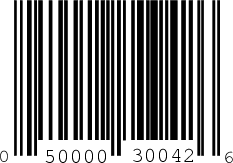
\includegraphics[width=\linewidth]{external/UPCcode.png}
\end{image}%
\tcblower
\end{figureptx}%
\end{divisionexercise}%
\begin{divisionexercise}{2}{}{}{groups-9-3}%
It is often useful to use an inner product notation for this type of error detection scheme; hence, we will use the notion%
\begin{equation*}
(d_1, d_2, \ldots, d_k ) \cdot (w_1, w_2, \ldots, w_k ) \equiv 0 \pmod{ n }
\end{equation*}
to mean%
\begin{equation*}
d_1 w_1 +  d_2 w_2 + \cdots +  d_k w_k  \equiv 0  \pmod{ n}\text{.}
\end{equation*}
%
\par
Suppose that \((d_1, d_2, \ldots, d_k ) \cdot (w_1, w_2, \ldots, w_k ) \equiv 0 \pmod{ n}\) is an error detection scheme for the \(k\)-digit identification number \(d_1 d_2 \cdots d_k\), where \(0 \leq d_i \lt n\).  Prove that all single-digit errors are detected if and only if \(\gcd( w_i, n ) = 1\) for  \(1 \leq i \leq k\).%
\end{divisionexercise}%
\begin{divisionexercise}{3}{}{}{groups-9-4}%
Let \((d_1, d_2, \ldots, d_k ) \cdot (w_1, w_2, \ldots, w_k ) \equiv 0 \pmod{ n}\) be an error detection scheme for the \(k\)-digit identification number \(d_1 d_2 \cdots d_k\), where \(0 \leq d_i \lt n\).  Prove that all transposition errors of two digits \(d_i\) and \(d_j\) are detected if and only if \(\gcd( w_i - w_j, n ) = 1\) for \(i\) and  \(j\) between 1 and \(k\).%
\end{divisionexercise}%
\begin{divisionexercise}{4}{ISBN Codes.}{}{groups-9-5}%
Every book has an International Standard Book Number\index{International standard book number} (ISBN) code.  This is a 10-digit code indicating the book's publisher and title.  The tenth digit is a check digit satisfying%
\begin{equation*}
(d_1, d_2, \ldots, d_{10} ) \cdot (10, 9, \ldots, 1 )  \equiv 0 \pmod{11}\text{.}
\end{equation*}
One problem is that \(d_{10}\) might have to be a 10 to make the inner product zero; in this case, 11 digits would be  needed to make this scheme work.  Therefore, the character X is used for the eleventh digit.  So ISBN 3-540-96035-X is a valid ISBN code.%
%
\begin{enumerate}[label={(\alph*)}]
\item{}Is ISBN 0-534-91500-0 a valid ISBN code?  What about ISBN 0-534-91700-0 and ISBN 0-534-19500-0?%
\item{}Does this method detect all single-digit errors?  What about all transposition errors?%
\item{}How many different ISBN codes are there?%
\item{}Write a computer program that will calculate the check digit for the first nine digits of an ISBN code.%
\item{}A publisher has houses in Germany and the United States.  Its German prefix is \mono{3-540}.  If its United States prefix will be \mono{0-abc}, find \mono{abc} such that the rest of the ISBN code will be the same for a book printed in Germany and in the United States. Under the ISBN coding method the first digit identifies the language; German is \mono{3} and English is \mono{0}.  The next group of numbers identifies the publisher, and the last group identifies the specific book.%
\end{enumerate}
\end{divisionexercise}%
\end{exercises-section}
%
%
\typeout{************************************************}
\typeout{Exercises 3.7 Sage Exercises}
\typeout{************************************************}
%
\begin{exercises-section}{Exercises}{Sage Exercises}{}{Sage Exercises}{}{}{groups-sage-exercises}
\begin{introduction}{}%
These exercises are about becoming comfortable working with groups in Sage.%
\end{introduction}%
\begin{divisionexercise}{1}{}{}{groups-sage-exercises-3}%
Create the groups \mono{CyclicPermutationGroup(8)} and \mono{DihedralGroup(4)} and name these groups \mono{C} and \mono{D}, respectively.  We will understand these constructions better shortly, but for now just understand that both objects you create are actually groups.%
\end{divisionexercise}%
\begin{divisionexercise}{2}{}{}{groups-sage-exercises-4}%
Check that \mono{C} and \mono{D} have the same size by using the \mono{.order()} method.  Determine which group is abelian, and which is not, by using the \mono{.is\_abelian()} method.%
\end{divisionexercise}%
\begin{divisionexercise}{3}{}{}{groups-sage-exercises-5}%
Use the \mono{.cayley\_table()} method to create the Cayley table for each group.%
\end{divisionexercise}%
\begin{divisionexercise}{4}{}{}{groups-sage-exercises-6}%
Write a nicely formatted discussion identifying differences between the two groups that are discernible in properties of their Cayley tables.  In other words, what is \textbraceleft{}\textbackslash{}em different\textbraceright{} about these two groups that you can ``see'' in the Cayley tables?  (In the Sage notebook, a Shift-click on a blue bar will bring up a mini-word-processor, and you can use use dollar signs to embed mathematics formatted using \TeX{} syntax.)%
\end{divisionexercise}%
\begin{divisionexercise}{5}{}{}{groups-sage-exercises-7}%
For \mono{C} locate the one subgroup of order \(4\).  The group \mono{D} has three subgroups of order \(4\).  Select one of the three subgroups of \mono{D} that has a different structure than the subgroup you obtained from \mono{C}.%
\par
The \mono{.subgroups()} method will give you a list of all of the subgroups to help you get started.  A Cayley table will help you tell the difference between the two subgroups.  What properties of these tables did you use to determine the difference in the structure of the subgroups?%
\end{divisionexercise}%
\begin{divisionexercise}{6}{}{}{groups-sage-exercises-8}%
The \mono{.subgroup(elt\_list)} method of a group will create the smallest subgroup containing the specified elements of the group, when given the elements as a list \mono{elt\_list}.  Use this command to discover the shortest list of elements necessary to recreate the subgroups you found in the previous exercise.  The equality comparison, \mono{==}, can be used to test if two subgroups are equal.%
\end{divisionexercise}%
\end{exercises-section}
%
%
\typeout{************************************************}
\typeout{References 3.8 References and Suggested Readings}
\typeout{************************************************}
%
\begin{references-section}{References}{References and Suggested Readings}{}{References and Suggested Readings}{}{}{groups-11}
%% If this is a top-level references
%%   you can replace the "referencelist" environment
%%   with a standard "thebibliography" environment
\begin{referencelist}
\bibitem[1]{groups-11-2}\hypertarget{groups-11-2}{}Burnside, W. \textit{Theory of Groups of Finite Order}. 2nd ed. Cambridge University Press, Cambridge, 1911; Dover, New York, 1953.  A classic.  Also available at books.google.com.
\bibitem[2]{groups-11-3}\hypertarget{groups-11-3}{}Gallian, J. A. and Winters, S. ``Modular Arithmetic in the Marketplace,'' \textit{The American Mathematical Monthly} \textbf{95} (1988): 548\textendash{}51.
\bibitem[3]{groups-11-4}\hypertarget{groups-11-4}{}Gallian, J. A. \textit{Contemporary Abstract Algebra}. 7th ed. Brooks\slash{}Cole, Belmont, CA, 2009.
\bibitem[4]{groups-11-5}\hypertarget{groups-11-5}{}Hall, M. \textit{Theory of Groups}. 2nd ed. American Mathematical Society, Providence, 1959.
\bibitem[5]{groups-11-6}\hypertarget{groups-11-6}{}Kurosh, A. E. \textit{The Theory of Groups}, vols. I and II. American Mathematical Society, Providence, 1979.
\bibitem[6]{groups-11-7}\hypertarget{groups-11-7}{}Rotman, J. J. \textit{An Introduction to the Theory of Groups}. 4th ed. Springer, New York, 1995.
\end{referencelist}
\end{references-section}
\end{chapterptx}
%
%
\typeout{************************************************}
\typeout{Chapter 4 Cyclic Groups}
\typeout{************************************************}
%
\begin{chapterptx}{Chapter}{Cyclic Groups}{}{Cyclicity}{}{}{cyclic}
\renewcommand*{\chaptername}{Chapter}
\begin{introduction}{}%
The groups \(\mathbb Z\) and \({\mathbb Z}_n\), which are among the most familiar and easily understood groups, are both examples of what are called cyclic groups.  In this chapter we will study the properties of cyclic groups and cyclic subgroups, which play a fundamental part in the classification of all abelian groups.%
\end{introduction}%
%
%
\typeout{************************************************}
\typeout{Section 4.1 Cyclic groups}
\typeout{************************************************}
%
\begin{sectionptx}{Section}{Cyclic groups}{}{Cyclic groups}{}{}{cyclic-4}
Often a subgroup will depend entirely on a single element of the group; that is, knowing that particular element will allow us to compute any other element in the subgroup.%
\begin{example}{Example}{An Infinite Cyclic Subgroup, Modular Addition.}{example-cyclic-z3}%
Suppose that we consider \(3 \in {\mathbb Z}\) and look at all multiples (both positive and negative) of 3.  As a set, this is%
\begin{equation*}
3 {\mathbb Z} = \{ \ldots, -3, 0, 3, 6, \ldots \}\text{.}
\end{equation*}
It is easy to see that \(3 {\mathbb Z}\) is a subgroup of the integers.  This subgroup is completely determined by the element 3 since we can obtain all of the other elements of the group by taking multiples of 3.  Every element in the subgroup is ``generated'' by 3.%
\end{example}
\begin{example}{Example}{An Infinite Cyclic Subgroup, Multiplication of Rational Numbers.}{example-cyclic-2n}%
If \(H = \{ 2^n : n \in {\mathbb Z} \}\), then \(H\) is a subgroup of the multiplicative group of nonzero rational numbers, \({\mathbb Q}^*\).  If \(a = 2^m\) and \(b = 2^n\) are in \(H\), then \(ab^{-1} = 2^m 2^{-n} = 2^{m-n}\) is also in \(H\).  By \hyperref[proposition-subgroup]{Proposition~{\xreffont\ref{proposition-subgroup}}}, \(H\) is a subgroup of \({\mathbb Q}^*\) determined by the element 2.%
\end{example}
\begin{theorem}{Theorem}{}{}{theorem-cyclic-subgroup}%
Let \(G\) be a group and \(a\) be any element in \(G\).  Then the set%
\begin{equation*}
\langle a \rangle  = \{ a^k : k \in {\mathbb Z} \}
\end{equation*}
is a subgroup of \(G\).  Furthermore, \(\langle a \rangle\) is the smallest subgroup of \(G\) that contains\textasciitilde{}\(a\).\label{theorem-cyclic-subgroup-1-1-9}%
\end{theorem}
\begin{proof}{Proof}{}{theorem-cyclic-subgroup-2}
The identity is in \(\langle a \rangle \) since \(a^0 = e\). If \(g\) and \(h\) are any two elements in \(\langle a \rangle \), then by the definition of \(\langle a \rangle\) we can write \(g = a^m\) and \(h = a^n\) for some integers \(m\) and \(n\). So \(gh = a^m a^n = a^{m+n}\) is again in \(\langle a \rangle \). Finally, if \(g = a^n\) in \(\langle a \rangle \), then the inverse \(g^{-1} = a^{-n}\) is also in \(\langle a \rangle \). Clearly, any subgroup \(H\) of \(G\) containing \(a\) must contain all the powers of \(a\) by closure; hence, \(H\) contains \(\langle a \rangle \). Therefore, \(\langle a \rangle \) is the smallest subgroup of \(G\) containing \(a\).%
\end{proof}
\begin{remark}{Remark}{}{cyclic-4-6}%
If we are using the ``+'' notation, as in the case of the integers under addition, we write \(\langle a \rangle  = \{ na : n \in {\mathbb Z} \}\).%
\end{remark}
For \(a \in G\), we call \(\langle a \rangle \) the \terminology{cyclic subgroup}\index{Subgroup!cyclic} generated by \(a\). If \(G\) contains some element \(a\) such that \(G = \langle a \rangle \), then \(G\) is a \terminology{cyclic group}\index{Group!cyclic}. In this case \(a\) is a \terminology{generator}\index{Generator of a cyclic subgroup} of \(G\).  If \(a\) is an element of a group \(G\), we define the \terminology{order}\index{Element!order of} of \(a\) to be the smallest positive integer \(n\) such that \(a^n= e\), and we write \(|a| = n\). \label{cyclic-4-7-24} If there is no such integer \(n\), we say that the order of \(a\) is infinite and  write \(|a| = \infty\) to denote the order of \(a\).%
\begin{example}{Example}{Generators of a Finite Cyclic Group.}{example-cyclic-z6}%
Notice that a cyclic group can have more than a single generator. Both 1 and 5 generate \({\mathbb Z}_6\); hence, \({\mathbb Z}_6\) is a cyclic group. Not every element in a cyclic group is necessarily a generator of the group. The order of \(2 \in {\mathbb Z}_6\) is 3. The cyclic subgroup generated by 2 is \(\langle 2 \rangle  = \{ 0, 2, 4 \}\).%
\end{example}
The groups \({\mathbb Z}\) and \({\mathbb Z}_n\) are cyclic groups. The elements 1 and \(-1\) are generators for \({\mathbb Z}\).  We can certainly generate \({\mathbb Z}_n\) with 1 although there may be other generators of \({\mathbb Z}_n\), as in the case of \({\mathbb Z}_6\).%
\begin{example}{Example}{A Cyclic Group of Units.}{example-cyclic-u9}%
The group of units, \(U(9)\), in \({\mathbb Z}_9\) is a cyclic group.  As a set, \(U(9)\) is \(\{ 1, 2, 4, 5, 7, 8  \}\). The element 2 is a generator for \(U(9)\) since%
\begin{align*}
2^1 & = 2 \qquad 2^2 = 4\\
2^3 & = 8 \qquad 2^4 = 7\\
2^5 & =  5 \qquad 2^6 = 1\text{.}
\end{align*}
%
\end{example}
\begin{example}{Example}{A Group That is Not Cyclic.}{example-cyclic-s3-not-cyclic}%
Not every group is a cyclic group.  Consider the symmetry group of an equilateral triangle \(S_3\).  The subgroups of \(S_3\) are shown in \hyperref[figure-subgrps-s3]{Figure~{\xreffont\ref{figure-subgrps-s3}}}.  Notice that every subgroup is cyclic; however, no single element generates the entire group.%
\end{example}
\begin{figureptx}{Figure}{Subgroups of \(S_3\)}{figure-subgrps-s3}{}%
\begin{image}{0}{1}{0}{}%
\resizebox{\linewidth}{!}{%
\begin{tikzpicture}[scale=1]

\draw  (0,0.3) -- (2.6,1.2);
\draw  (2,0.3) -- (2.8,1.2);
\draw  (4,0.3) -- (3.2,1.2);
\draw  (6,0.3) -- (3.4,1.2);

\draw  (0,-0.3) -- (2.6,-1.2);
\draw  (2,-0.3) -- (2.8,-1.2);
\draw  (4,-0.3) -- (3.2,-1.2);
\draw  (6,-0.3) -- (3.4,-1.2);

\node at (0, 0) {$\{  \identity, \rho_1, \rho_2\}$};
\node at (2, 0) {$\{  \identity, \mu_1\}$};
\node at (4, 0) {$\{  \identity, \mu_2 \}$};
\node at (6, 0) {$\{  \identity, \mu_3 \}$};
\node at (3, 1.5) {$S_3$};
\node at (3,-1.5) {$\{ \identity \}$};
\end{tikzpicture}%
}%
\end{image}%
\tcblower
\end{figureptx}%
\begin{theorem}{Theorem}{}{}{theorem-cyclic-abelian}%
Every cyclic group is abelian.%
\end{theorem}
\begin{proof}{Proof}{}{theorem-cyclic-abelian-2}
Let \(G\) be a cyclic group and \(a \in G\) be a generator for \(G\). If \(g\) and \(h\) are in \(G\), then they can be written as powers of \(a\), say \(g = a^r\) and \(h = a^s\). Since%
\begin{equation*}
g  h = a^r a^s = a^{r+s} = a^{s+r} = a^s a^r = h g\text{,}
\end{equation*}
\(G\) is abelian.%
\end{proof}
\end{sectionptx}
%
%
\typeout{************************************************}
\typeout{Section 4.2 Subgroups of a Cyclic Group}
\typeout{************************************************}
%
\begin{sectionptx}{Section}{Subgroups of a Cyclic Group}{}{Subgroups of a Cyclic Group}{}{}{cyclic-5}
We can ask some interesting questions about cyclic subgroups of a group and subgroups of a cyclic group.  If \(G\) is a group, which subgroups of \(G\) are cyclic? If \(G\) is a cyclic group, what type of subgroups does \(G\) possess?%
\begin{theorem}{Theorem}{}{}{theorem-cyclic-subgroups}%
Every subgroup of a cyclic group is cyclic.%
\end{theorem}
\begin{proof}{Proof}{}{theorem-cyclic-subgroups-2}
The main tools used in this proof are the division algorithm and the Principle of Well-Ordering. Let \(G\) be a cyclic group generated by \(a\) and suppose that \(H\) is a subgroup of \(G\). If \(H = \{ e \}\), then trivially \(H\) is cyclic. Suppose that \(H\) contains some other element \(g\) distinct from the identity. Then \(g\) can be written as \(a^n\) for some integer \(n\). Since \(H\) is a subgroup, \(g^{-1} = a^{n}\) must also be in \(H\).  Since either \(n\) or \(-n\) is positive, we can assume that \(H\) contains positive powers of \(a\) and \(n \gt 0\). Let \(m\) be the smallest natural number such that \(a^m \in H\). Such an \(m\) exists by the Principle of Well-Ordering.%
\par
We claim that \(h = a^m\) is a generator for \(H\).  We must show that every \(h' \in H\) can be written as a power of \(h\). Since \(h' \in H\) and \(H\) is a subgroup of \(G\), \(h' = a^k\) for some integer \(k\). Using the division algorithm, we can find numbers \(q\) and \(r\) such that \(k = mq +r\) where \(0 \leq r \lt m\); hence,%
\begin{equation*}
a^k = a^{mq +r} = (a^m)^q a^r = h^q a^r\text{.}
\end{equation*}
So \(a^r = a^k h^{-q}\). Since \(a^k\) and \(h^{-q}\) are in \(H\), \(a^r\) must also be in \(H\).  However, \(m\) was the smallest positive number such that \(a^m\) was in \(H\); consequently, \(r=0\) and so \(k=mq\). Therefore,%
\begin{equation*}
h' = a^k = a^{mq} =  h^q
\end{equation*}
and \(H\) is generated by \(h\).%
\end{proof}
\begin{corollary}{Corollary}{}{}{cyclic-5-4}%
The subgroups of \({\mathbb Z}\) are exactly \(n{\mathbb Z}\) for \(n = 0, 1, 2,\ldots\).%
\end{corollary}
\begin{proposition}{Proposition}{}{}{proposition-cyclic-subgrp-order}%
Let \(G\) be a cyclic group of order \(n\) and suppose that \(a\) is a generator for  \(G\). Then \(a^k=e\) if and only if \(n\) divides \(k\).%
\end{proposition}
\begin{proof}{Proof}{}{proposition-cyclic-subgrp-order-2}
First suppose that \(a^k=e\). By the division algorithm, \(k = nq + r\) where \(0 \leq r \lt n\); hence,%
\begin{equation*}
e = a^k = a^{nq + r} = a^{nq} a^r = e a^r = a^r\text{.}
\end{equation*}
Since the smallest positive integer \(m\) such that \(a^m = e\) is \(n\), \(r= 0\).%
\par
Conversely, if \(n\) divides \(k\), then \(k=ns\) for some integer \(s\). Consequently,%
\begin{equation*}
a^k = a^{ns} = (a^n)^s = e^s = e\text{.}
\end{equation*}
%
\end{proof}
\begin{theorem}{Theorem}{}{}{theorem-cyclic-orders}%
Let \(G\) be a cyclic group of order \(n\) and suppose that \(a \in G\) is a generator of the group.  If \(b = a^k\), then the order of \(b\) is \(n/d\), where \(d = \gcd(k,n)\).%
\end{theorem}
\begin{proof}{Proof}{}{theorem-cyclic-orders-2}
We wish to find the smallest integer \(m\) such that \(e = b^m = a^{km}\). By \hyperref[proposition-cyclic-subgrp-order]{Proposition~{\xreffont\ref{proposition-cyclic-subgrp-order}}}, this is the smallest integer \(m\) such that \(n\) divides \(km\) or, equivalently, \(n/d\) divides \(m(k/d)\).  Since \(d\) is the greatest common divisor of \(n\) and \(k\), \(n/d\) and \(k/d\) are relatively prime. Hence, for \(n/d\) to divide \(m(k/d)\) it must divide \(m\).  The smallest such \(m\) is \(n/d\).%
\end{proof}
\begin{corollary}{Corollary}{}{}{corollary-cyclic-modngenerators}%
The generators of \({\mathbb Z}_n\) are the integers \(r\) such that \(1 \leq r \lt n\) and \(\gcd(r,n) =  1\).%
\end{corollary}
\begin{example}{Example}{A Finite Cyclic Group of Order \(16\).}{example-cyclic-z16}%
Let us examine the group \({\mathbb Z}_{16}\).  The numbers 1, 3, 5, 7, 9, 11, 13, and 15 are the elements of \({\mathbb Z}_{16}\) that are relatively prime to 16.  Each of these elements generates \({\mathbb Z}_{16}\). For example,%
\begin{align*}
1 \cdot 9  & =  9  &  2 \cdot 9  & = 2  & 3 \cdot 9  & = 11\\
4 \cdot 9  & =  4  &  5 \cdot 9  & = 13 &     6 \cdot 9 & = 6\\
7 \cdot 9  & =  15 & 8 \cdot 9  & = 8  &  9 \cdot 9 &  = 1\\
10 \cdot 9 & =  10 & 11 \cdot 9 & = 3  & 12 \cdot 9 &  = 12\\
13 \cdot 9 & =  5 & 14 \cdot 9 & = 14 &   15 \cdot 9 & = 7\text{.}
\end{align*}
%
\end{example}
\end{sectionptx}
%
%
\typeout{************************************************}
\typeout{Section 4.3 Cyclic Groups of Complex Numbers}
\typeout{************************************************}
%
\begin{sectionptx}{Section}{Cyclic Groups of Complex Numbers}{}{Cyclic Groups of Complex Numbers}{}{}{cyclic-6}
The \terminology{complex numbers} are defined as%
\begin{equation*}
{\mathbb C} = \{ a + bi : a, b \in {\mathbb R} \}\text{,}
\end{equation*}
where \(i^2 = -1\).  If \(z = a + bi\), then \(a\) is the \terminology{real part} of \(z\) and \(b\) is the \terminology{imaginary part} of \(z\).%
\par
To add two complex numbers \(z=a+bi\) and \(w= c+di\), we just add the corresponding real and imaginary parts:%
\begin{equation*}
z + w=(a + bi ) + (c + di)  =  (a + c) + (b + d)i\text{.}
\end{equation*}
Remembering that \(i^2 = -1\),  we multiply complex numbers just like polynomials. The product of \(z\) and \(w\) is%
\begin{equation*}
(a + bi )(c + di)  =   ac + bdi^2 + adi + bci =  (ac -bd) +(ad + bc)i\text{.}
\end{equation*}
%
\par
Every nonzero complex number \(z = a +bi\) has a multiplicative inverse; that is, there exists a \(z^{-1} \in {\mathbb C}^\ast\) such that \(z z^{-1} = z^{-1} z = 1\). If \(z = a + bi\), then%
\begin{equation*}
z^{-1} = \frac{a-bi}{ a^2 + b^2  }\text{.}
\end{equation*}
The \terminology{complex conjugate}\index{Conjugate, complex} of a complex number \(z = a + bi\) is defined to be \(\overline{z} = a- bi\).  The \terminology{absolute value} or \terminology{modulus} of  \(z = a + bi\)  is \(|z| = \sqrt{a^2 + b^2}\).%
\begin{example}{Example}{Complex Number Operations.}{example-cyclic-complex-add}%
Let \(z = 2 + 3i\) and \(w = 1-2i\). Then%
\begin{equation*}
z + w = (2 + 3i) + (1 - 2i) = 3 + i
\end{equation*}
and%
\begin{equation*}
z  w = (2 + 3i)(1 - 2i ) = 8 - i\text{.}
\end{equation*}
Also,%
\begin{align*}
z^{-1} & = \frac{2}{13} - \frac{3}{13}i\\
|z| & = \sqrt{13}\\
\overline{z} & = 2-3i\text{.}
\end{align*}
%
\end{example}
\begin{figureptx}{Figure}{Rectangular coordinates of a complex number}{figure-rectcoord}{}%
\begin{image}{0}{1}{0}{}%
\resizebox{\linewidth}{!}{%
\begin{tikzpicture}[scale=0.5]

\draw [->]  (0,-5) -- (0,5);
\draw  [->] (-8,0) -- (8,0);
\node [right] at (0,5) {$y$};
\node [below] at (8,0) {$x$};
\node [below] at (0.5,0) {$0$};

\filldraw[fill=black, draw=black] (2,3) circle (0.05cm);
\node [right] at (2,3) {$z_1 = 2 + 3i$};

\filldraw[fill=black, draw=black] (-3,2) circle (0.05cm);
\node [left] at (-3, 2) {$z_3 = -3 + 2i$};

\filldraw[fill=black, draw=black] (1,-2) circle (0.05cm);
\node [right] at (1, -2) {$z_2 = 1 -  2i$};

\end{tikzpicture}%
}%
\end{image}%
\tcblower
\end{figureptx}%
There are several ways of graphically representing complex numbers. We can represent a complex number \(z = a +bi\) as an ordered pair on the \(xy\) plane where \(a\) is the \(x\) (or real) coordinate and \(b\) is the \(y\) (or imaginary) coordinate. This is called the \terminology{rectangular} or \terminology{Cartesian} representation. The rectangular representations of \(z_1 = 2 + 3i\), \(z_2 = 1 - 2i\), and \(z_3 = - 3 + 2i\) are depicted in \hyperref[figure-rectcoord]{Figure~{\xreffont\ref{figure-rectcoord}}}.%
\begin{figureptx}{Figure}{Polar coordinates of a complex number}{figure-polarcoord}{}%
\begin{image}{0}{1}{0}{}%
\resizebox{\linewidth}{!}{%
\begin{tikzpicture}[scale=0.5]

\draw [->]  (0,-5) -- (0,5);
\draw  [->] (-8,0) -- (8,0);
\node [right] at (0,5) {$y$};
\node [below] at (8,0) {$x$};
\node [below] at (0.5,0) {$0$};

\draw (0,0) -- (35:6);
\draw (2,0) arc (0:35:2);

\filldraw[fill=black, draw=black] (35:6) circle (0.05cm);
\node [right] at (35:6) {$a + bi$};
\node [above] at (35:3) {$r$};
\node [right] at (17:2) {$\theta$};

\end{tikzpicture}%
}%
\end{image}%
\tcblower
\end{figureptx}%
Nonzero complex numbers can also be represented using \terminology{polar coordinates}.  To specify  any nonzero point on the plane, it suffices to give an angle \(\theta\) from the positive \(x\) axis in the counterclockwise direction and a distance \(r\) from the origin, as in \hyperref[figure-polarcoord]{Figure~{\xreffont\ref{figure-polarcoord}}}. We can see that%
\begin{equation*}
z = a + bi = r( \cos \theta + i \sin \theta)\text{.}
\end{equation*}
Hence,%
\begin{equation*}
r = |z| = \sqrt{a^2 + b^2}
\end{equation*}
and%
\begin{align*}
a & = r \cos \theta\\
b & = r \sin \theta\text{.}
\end{align*}
We sometimes abbreviate \(r( \cos \theta + i \sin \theta)\) as \(r \cis \theta\).  To assure that the representation of \(z\) is  well-defined, we also require that \(0^{\circ} \leq \theta \lt 360^{\circ}\).  If the measurement is in radians, then \(0 \leq \theta \lt2 \pi\).\label{cyclic-6-9-14}%
\begin{example}{Example}{Complex Numbers in Polar Form.}{example-cyclic-polar}%
Suppose that \(z = 2 \cis  60^{\circ}\). Then%
\begin{equation*}
a = 2 \cos 60^{\circ} = 1
\end{equation*}
and%
\begin{equation*}
b = 2 \sin 60^{\circ} = \sqrt{3}\text{.}
\end{equation*}
Hence, the rectangular representation is \(z = 1+\sqrt{3}\, i\).%
\par
Conversely, if we are given a rectangular representation of a complex number, it is often useful to know the number's polar representation. If \(z = 3 \sqrt{2} - 3 \sqrt{2}\, i\), then%
\begin{equation*}
r = \sqrt{a^2 + b^2} = \sqrt{36 } = 6
\end{equation*}
and%
\begin{equation*}
\theta = \arctan \left( \frac{b}{a} \right) = \arctan( - 1) = 315^{\circ}\text{,}
\end{equation*}
so \(3 \sqrt{2} - 3 \sqrt{2}\, i=6 \cis  315^{\circ}\).%
\end{example}
The polar representation of a complex number makes it easy to find products and powers of complex numbers.  The proof of the following proposition is straightforward and is left as an exercise.%
\begin{proposition}{Proposition}{}{}{proposition-polar-mult}%
Let \(z = r \cis \theta\) and \(w = s \cis \phi\) be two nonzero complex numbers. Then%
\begin{equation*}
zw = r s \cis( \theta + \phi)\text{.}
\end{equation*}
%
\end{proposition}
\begin{example}{Example}{Multiplication of Complex Numbers in Polar Form.}{example-cyclic-polar-mult}%
If \(z =  3 \cis( \pi / 3 )\) and \(w = 2 \cis(\pi / 6 )\), then \(zw = 6 \cis( \pi / 2 ) = 6i\).%
\end{example}
\begin{theorem}{Theorem}{DeMoivre.}{}{theorem-demoivre}%
\index{DeMoivre's Theorem}%
Let \(z = r \cis  \theta\) be a nonzero complex number. Then%
\begin{equation*}
[r \cis \theta  ]^n = r^n \cis( n \theta)
\end{equation*}
for \(n = 1, 2, \ldots\).%
\end{theorem}
\begin{proof}{Proof}{}{theorem-demoivre-4}
We will use induction on \(n\) (see \hyperref[section-math-induction]{Section~{\xreffont\ref{section-math-induction}}}). For \(n = 1\) the theorem is trivial. Assume that the theorem is true for all \(k\) such that \(1  \leq k \leq n\). Then%
\begin{align*}
z^{n+1} & = z^n z\\
& = r^n( \cos  n \theta + i \sin n \theta ) r( \cos \theta + i\sin \theta )\\
& = r^{n+1} [( \cos n \theta \cos \theta - \sin n \theta \sin \theta ) + i ( \sin n \theta \cos \theta + \cos n \theta \sin \theta)]\\
& = r^{n+1} [ \cos( n \theta + \theta) + i \sin( n \theta + \theta) ]\\
& = r^{n+1} [ \cos( n +1) \theta + i \sin( n+1) \theta  ]\text{.}
\end{align*}
%
\end{proof}
\begin{example}{Example}{Powers of Complex Numbers.}{cyclic-6-15}%
Suppose that \(z= 1+i\) and we wish to compute \(z^{10}\). Rather than computing \((1 + i)^{10}\) directly, it is much easier to switch to polar coordinates and calculate \(z^{10}\) using DeMoivre's Theorem:%
\begin{align*}
z^{10} & = (1+i)^{10}\\
& = \left( \sqrt{2} \cis \left( \frac{\pi }{4} \right) \right)^{10}\\
& = ( \sqrt{2}\, )^{10} \cis \left( \frac{5\pi }{2} \right)\\
& = 32  \cis \left( \frac{\pi }{2} \right)\\
& = 32i\text{.}
\end{align*}
%
\end{example}
The multiplicative group of the complex numbers, \({\mathbb C}^*\), possesses some interesting subgroups.  Whereas \({\mathbb Q}^*\) and \({\mathbb R}^*\) have no interesting subgroups of finite order, \({\mathbb C}^*\) has many. We first consider the \terminology{circle group}\index{Group!circle},%
\begin{equation*}
{\mathbb T} = \{ z \in {\mathbb C} : |z| = 1 \}\text{.}
\end{equation*}
The following proposition is a direct result of \hyperref[proposition-polar-mult]{Proposition~{\xreffont\ref{proposition-polar-mult}}}.\label{cyclic-6-16-9}%
\begin{proposition}{Proposition}{}{}{cyclic-6-17}%
The circle group is a subgroup of  \({\mathbb C}^*\).%
\end{proposition}
Although the circle group has infinite order, it has many interesting finite subgroups. Suppose that \(H = \{ 1, -1, i, -i \}\). Then \(H\) is a subgroup of the circle group. Also, \(1\), \(-1\), \(i\), and \(-i\) are exactly those complex numbers that satisfy the equation \(z^4 = 1\). The complex numbers satisfying the equation \(z^n=1\) are called the \terminology{\(n\)th roots of unity}\index{\(n\)th root of unity}.%
\begin{theorem}{Theorem}{}{}{cyclic-6-19}%
If \(z^n = 1\), then the \(n\)th roots of unity are%
\begin{equation*}
z = \cis\left( \frac{2 k \pi}{n } \right)\text{,}
\end{equation*}
where \(k = 0, 1, \ldots, n-1\). Furthermore, the \(n\)th roots of unity form a cyclic subgroup of \({\mathbb T}\) of order \(n\)%
\end{theorem}
\begin{proof}{Proof}{}{cyclic-6-19-2}
By DeMoivre's Theorem,%
\begin{equation*}
z^n = \cis \left( n \frac{2 k \pi}{n } \right) = \cis( 2 k \pi ) = 1\text{.}
\end{equation*}
The \(z\)'s are distinct since the numbers \(2 k \pi /n\) are all distinct and are greater than or equal to 0 but less than \(2 \pi\).  We will leave the proof that the \(n\)th roots of unity form a cyclic subgroup of \({\mathbb T}\) as an exercise.%
\end{proof}
A generator for the group of the \(n\)th roots of unity is called a \terminology{primitive \(n\)th root of unity}\index{Primitive \(n\)th root of unity}.%
\begin{example}{Example}{Roots of Unity.}{example-roots_unity}%
The 8th roots of unity can be represented as eight equally spaced points on the unit circle (\hyperref[figure-rtsunity]{Figure~{\xreffont\ref{figure-rtsunity}}}).  The primitive 8th roots of unity are%
\begin{align*}
\omega & = \frac{\sqrt{2}}{2}  + \frac{\sqrt{2}}{2} i\\
\omega^3 & = -\frac{\sqrt{2}}{2}  + \frac{\sqrt{2}}{2} i\\
\omega^5 & = -\frac{\sqrt{2}}{2}  - \frac{\sqrt{2}}{2} i\\
\omega^7 & = \frac{\sqrt{2}}{2}  - \frac{\sqrt{2}}{2}i. 
\end{align*}
%
\end{example}
\begin{figureptx}{Figure}{8th roots of unity}{figure-rtsunity}{}%
\begin{image}{0}{1}{0}{}%
\resizebox{\linewidth}{!}{%
% Cyclic 8-th roots of unity
% NB: comments are in TeX, not XML
%
\begin{tikzpicture}[scale=1.65]

\draw [->]  (0,-1.5) -- (0,1.5);
\draw  [->] (-1.75,0) -- (1.75,0);
\node [right] at (0,1.5) {$y$};
\node [below] at (1.75,0) {$x$};
\node [below] at (0.1,0) {$0$};

\draw (0,0) circle (1);

\filldraw[fill=black, draw=black] (0:1) circle (0.03);
\filldraw[fill=black, draw=black] (45:1) circle (0.03);
\filldraw[fill=black, draw=black] (90:1) circle (0.03);
\filldraw[fill=black, draw=black] (135:1) circle (0.03);
\filldraw[fill=black, draw=black] (180:1) circle (0.03);
\filldraw[fill=black, draw=black] (225:1) circle (0.03);
\filldraw[fill=black, draw=black] (270:1) circle (0.03);
\filldraw[fill=black, draw=black] (315:1) circle (0.03);


\node [right] at (1,-0.15) {1};
\node [right] at (45:1) {$\omega$};
\node [left] at (0,1.15) {$i$};
\node [left] at (135:1) {$\omega^3$};
\node [left] at (-1,-0.15) {$-1$};
\node [left] at (225:1) {$\omega^5$};
\node [left] at (0,-1.15) {$-i$};
\node [right] at (315:1) {$\omega^7$};

\end{tikzpicture}%
}%
\end{image}%
\tcblower
\end{figureptx}%
We interrupt this exposition to repeat the previous diagram, wrapped as different figure with a different caption.  The TikZ code to produce these diagrams lives in an external file, \mono{tikz/cyclic-roots-unity.tex}, which is pure text, freed from any need to format for XML processing.  So, in particular, there is no need to escape ampersands and angle brackets, nor is there employment of the \mono{CDATA} mechanism.  But the real value is that there is just one version to edit, and any changes will be reflected in both copies.%
\begin{figureptx}{Figure}{Repeat: 8th roots of unity}{figure-rtsunity-copy}{}%
\begin{image}{0}{1}{0}{}%
\resizebox{\linewidth}{!}{%
% Cyclic 8-th roots of unity
% NB: comments are in TeX, not XML
%
\begin{tikzpicture}[scale=1.65]

\draw [->]  (0,-1.5) -- (0,1.5);
\draw  [->] (-1.75,0) -- (1.75,0);
\node [right] at (0,1.5) {$y$};
\node [below] at (1.75,0) {$x$};
\node [below] at (0.1,0) {$0$};

\draw (0,0) circle (1);

\filldraw[fill=black, draw=black] (0:1) circle (0.03);
\filldraw[fill=black, draw=black] (45:1) circle (0.03);
\filldraw[fill=black, draw=black] (90:1) circle (0.03);
\filldraw[fill=black, draw=black] (135:1) circle (0.03);
\filldraw[fill=black, draw=black] (180:1) circle (0.03);
\filldraw[fill=black, draw=black] (225:1) circle (0.03);
\filldraw[fill=black, draw=black] (270:1) circle (0.03);
\filldraw[fill=black, draw=black] (315:1) circle (0.03);


\node [right] at (1,-0.15) {1};
\node [right] at (45:1) {$\omega$};
\node [left] at (0,1.15) {$i$};
\node [left] at (135:1) {$\omega^3$};
\node [left] at (-1,-0.15) {$-1$};
\node [left] at (225:1) {$\omega^5$};
\node [left] at (0,-1.15) {$-i$};
\node [right] at (315:1) {$\omega^7$};

\end{tikzpicture}%
}%
\end{image}%
\tcblower
\end{figureptx}%
Another version of this diagram, authored in PreFigure, is also included in \hyperref[prefigure-rtsunity]{Figure~{\xreffont\ref{prefigure-rtsunity}}}.%
\begin{figureptx}{Figure}{8th roots of unity, authored in PreFigure}{prefigure-rtsunity}{}%
\begin{image}{0.15}{0.7}{0.15}{}%
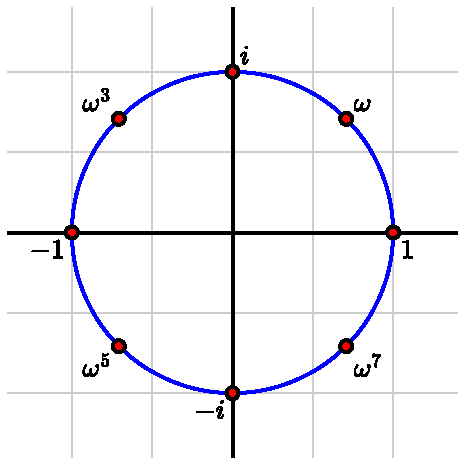
\includegraphics[width=\linewidth]{generated/prefigure/prefigure-rtsunity.pdf}%
\end{image}%
\tcblower
\end{figureptx}%
\end{sectionptx}
%
%
\typeout{************************************************}
\typeout{Section 4.4 Large Powers of Integers}
\typeout{************************************************}
%
\begin{sectionptx}{Section}{Large Powers of Integers}{}{Large Powers of Integers}{}{}{cyclic-7}
Computing large powers can be very time-consuming. Just as anyone can compute \(2^2\) or \(2^8\), everyone knows how to compute%
\begin{equation*}
2^{2^{1000000} }\text{.}
\end{equation*}
However, such numbers are so large that we do not want to attempt the calculations; moreover, past a certain point the computations would not be feasible even if we had every computer in the world at our disposal. Even writing down the decimal representation of a very large number may not be reasonable. It could be thousands or even millions of digits long. However, if we could compute something like \(2^{37398332 } \pmod{ 46389}\), we could very easily write the result down since it would be a number between 0 and 46,388. If we want to compute powers modulo \(n\) quickly and efficiently, we will have to be clever.\footnote{The results in this section are needed only in \hyperref[integers]{Chapter~{\xreffont\ref{integers}}} (not really).\label{cyclic-7-2-6}}%
\par
The first thing to notice is that any number \(a\) can be written as the sum of distinct powers of 2; that is, we can write%
\begin{equation*}
a = 2^{k_1} + 2^{k_2} + \cdots + 2^{k_n}\text{,}
\end{equation*}
where \(k_1 \lt k_2 \lt \cdots \lt k_n\).  This is just the binary representation of \(a\). For example, the binary representation of 57 is 111001, since we can write \(57 = 2^0 + 2^3 + 2^4 + 2^5\).%
\par
The laws of exponents still work in \({\mathbb Z}_n\); that is, if \(b \equiv a^x \pmod{ n}\) and \(c \equiv a^y \pmod{ n}\), then \(bc \equiv a^{x+y} \pmod{ n}\). We can compute \(a^{2^k} \pmod{ n}\) in \(k\) multiplications by computing%
\begin{gather*}
a^{2^0} \pmod{ n}\\
a^{2^1} \pmod{ n }\\
\vdots\\
a^{2^k} \pmod{ n}\text{.}
\end{gather*}
Each step involves squaring the answer obtained in the previous step, dividing by \(n\), and taking the remainder.%
\begin{example}{Example}{Repeated Squares.}{example-cyclic-repeated-squares}%
We will compute \(271^{321} \pmod{ 481}\). Notice that%
\begin{equation*}
321 = 2^0 +2^6 + 2^8\text{;}
\end{equation*}
hence, computing \(271^{321} \pmod{ 481}\) is the same as computing%
\begin{equation*}
271^{2^0 +2^6 + 2^8 } \equiv 271^{2^0} \cdot 271^{2^6} \cdot 271^{2^8} \pmod{481}\text{.}
\end{equation*}
So it will suffice to compute \(271^{2^i} \pmod{481}\) where \(i = 0, 6, 8\). It is very easy to see that%
\begin{equation*}
271^{2^1}  = \mbox{73,441} \equiv 329 \pmod{481}\text{.}
\end{equation*}
We can square this result to obtain a value for \(271^{2^2} \pmod{481}\):%
\begin{align*}
271^{ 2^2}  & \equiv (271^{ 2^1})^2 \pmod{ 481}\\
& \equiv (329)^2 \pmod{ 481}\\
& \equiv \mbox{108,241} \pmod{ 481}\\
& \equiv 16 \pmod{ 481}\text{.}
\end{align*}
We are using the fact that \((a^{2^n})^2  \equiv a^{2 \cdot 2^n} \equiv a^{ 2^{n+1} } \pmod{ n}\). Continuing, we can calculate%
\begin{equation*}
271^{ 2^6 } \equiv 419 \pmod{ 481}
\end{equation*}
and%
\begin{equation*}
271^{ 2^8 }  \equiv 16 \pmod{ 481}\text{.}
\end{equation*}
Therefore,%
\begin{align*}
271^{ 321} & \equiv 271^{ 2^0 +2^6 + 2^8 } \pmod{ 481}\\
& \equiv 271^{ 2^0 } \cdot 271^{ 2^6 } \cdot 271^{ 2^8 } \pmod{ 481}\\
& \equiv 271 \cdot 419 \cdot 16 \pmod{ 481}\\
& \equiv \mbox{1,816,784} \pmod{ 481}\\
& \equiv 47 \pmod{ 481}\text{.}
\end{align*}
%
\end{example}
The method of repeated squares will prove to be a very useful tool when we explore  \acronym{RSA} cryptography. To encode and decode messages in a reasonable manner under this scheme, it is necessary to be able to quickly compute large powers of integers mod \(n\).%
\begin{remark}{Remark}{Sage.}{cyclic-7-7}%
Sage support for cyclic groups is a little spotty \textemdash{} but we can still make effective use of Sage and perhaps this situation could change soon.%
\end{remark}
\end{sectionptx}
%
%
\typeout{************************************************}
\typeout{Exercises 4.5 Exercises}
\typeout{************************************************}
%
\begin{exercises-section}{Exercises}{Exercises}{}{Exercises}{}{}{exercises-cyclic}
\begin{divisionexercise}{1}{}{}{exercises-cyclic-2}%
Prove or disprove each of the following statements.%
%
\begin{enumerate}[label={(\alph*)}]
\item{}All of the generators of \({\mathbb Z}_{60}\) are prime.%
\item{}\(U(8)\) is cyclic.%
\item{}\({\mathbb Q}\) is cyclic.%
\item{}If every proper subgroup of a group \(G\) is cyclic, then \(G\) is a cyclic group.%
\item{}A group with a finite number of subgroups is finite.%
\end{enumerate}
\end{divisionexercise}%
\begin{divisionexercise}{2}{}{}{exercises-cyclic-3}%
Find the order of each of the following elements.%
%
\begin{multicols}{2}
\begin{enumerate}[label={(\alph*)}]
\item{}\(\displaystyle 5 \in {\mathbb Z}_{12}\)%
\item{}\(\displaystyle \sqrt{3} \in {\mathbb R}\)%
\item{}\(\displaystyle \sqrt{3} \in {\mathbb R}^\ast\)%
\item{}\(\displaystyle -i \in {\mathbb C}^\ast\)%
\item{}72 in \({\mathbb Z}_{240}\)%
\item{}312 in \({\mathbb Z}_{471}\)%
\end{enumerate}
\end{multicols}
\end{divisionexercise}%
\begin{divisionexercise}{3}{}{}{exercises-cyclic-4}%
List all of the elements in each of the following subgroups.%
%
\begin{enumerate}[label={(\alph*)}]
\item{}The subgroup of \({\mathbb Z}\) generated by 7%
\item{}The subgroup of \({\mathbb Z}_{24}\) generated by 15%
\item{}All subgroups of \({\mathbb Z}_{12}\)%
\item{}All subgroups of \({\mathbb Z}_{60}\)%
\item{}All subgroups of \({\mathbb Z}_{13}\)%
\item{}All subgroups of \({\mathbb Z}_{48}\)%
\item{}The subgroup generated by 3  in \(U(20)\)%
\item{}The subgroup generated by 5 in \(U(18)\)%
\item{}The subgroup of \({\mathbb R}^\ast\) generated by 7%
\item{}The subgroup of \({\mathbb C}^\ast\) generated by \(i\) where \(i^2 = -1\)%
\item{}The subgroup of \({\mathbb C}^\ast\) generated by \(2i\)%
\item{}The subgroup of \({\mathbb C}^\ast\) generated by \((1 + i) / \sqrt{2}\)%
\item{}The subgroup of \({\mathbb C}^\ast\) generated by \((1 + \sqrt{3}\, i) / 2\)%
\end{enumerate}
\end{divisionexercise}%
\begin{divisionexercise}{4}{}{}{exercises-cyclic-5}%
Find the subgroups of \(GL_2( {\mathbb R })\) generated by each of the following matrices.%
%
\begin{multicols}{3}
\begin{enumerate}[label={(\alph*)}]
\item{}\(\displaystyle \displaystyle \begin{pmatrix}
0 & 1 \\
-1 & 0
\end{pmatrix}\)%
\item{}\(\displaystyle \displaystyle
\begin{pmatrix}
0 & 1/3 \\
3 & 0
\end{pmatrix}\)%
\item{}\(\displaystyle \displaystyle
\begin{pmatrix}
1 & -1 \\
1 & 0
\end{pmatrix}\)%
\item{}\(\displaystyle \displaystyle
\begin{pmatrix}
1 & -1 \\
0 & 1
\end{pmatrix}\)%
\item{}\(\displaystyle \displaystyle
\begin{pmatrix}
1 & -1 \\
-1 & 0
\end{pmatrix}\)%
\item{}\(\displaystyle \displaystyle
\begin{pmatrix}
\sqrt{3}/ 2 & 1/2 \\
-1/2 & \sqrt{3}/2
\end{pmatrix}\)%
\end{enumerate}
\end{multicols}
\end{divisionexercise}%
\begin{divisionexercise}{5}{}{}{exercises-cyclic-6}%
Find the order of every element in \({\mathbb Z}_{18}\).%
\end{divisionexercise}%
\begin{divisionexercise}{6}{}{}{exercises-cyclic-7}%
Find the order of every element in the symmetry group of the square, \(D_4\).%
\end{divisionexercise}%
\begin{divisionexercise}{7}{}{}{exercises-cyclic-8}%
What are all of the cyclic subgroups of the quaternion group, \(Q_8\)?%
\end{divisionexercise}%
\begin{divisionexercise}{8}{}{}{exercises-cyclic-9}%
List all of the cyclic subgroups of \(U(30)\).%
\end{divisionexercise}%
\begin{divisionexercise}{9}{}{}{exercises-cyclic-10}%
List every generator of each subgroup of order 8 in \({\mathbb Z}_{32}\).%
\end{divisionexercise}%
\begin{divisionexercise}{10}{}{}{exercises-cyclic-11}%
Find all elements of finite order in each of the following groups. Here the ``\(\ast\)'' indicates the set with zero removed.%
%
\begin{multicols}{3}
\begin{enumerate}[label={(\alph*)}]
\item{}\(\displaystyle {\mathbb Z}\)%
\item{}\(\displaystyle {\mathbb Q}^\ast\)%
\item{}\(\displaystyle {\mathbb R}^\ast\)%
\end{enumerate}
\end{multicols}
\end{divisionexercise}%
\begin{divisionexercise}{11}{}{}{exercises-cyclic-12}%
If \(a^{24} =e\) in a group \(G\), what are the possible orders of \(a\)?%
\end{divisionexercise}%
\begin{divisionexercise}{12}{}{}{exercises-cyclic-13}%
Find a cyclic group with exactly one generator. Can you find cyclic groups with exactly two generators? Four generators? How about \(n\) generators?%
\end{divisionexercise}%
\begin{divisionexercise}{13}{}{}{exercises-cyclic-14}%
For \(n \leq 20\), which groups \(U(n)\) are cyclic?  Make a conjecture as to what is true in general.  Can you prove your conjecture?%
\end{divisionexercise}%
\begin{divisionexercise}{14}{}{}{exercises-cyclic-15}%
Let%
\begin{equation*}
A =
\begin{pmatrix}
0 & 1 \\
-1 & 0
\end{pmatrix}
\qquad \text{and} \qquad
B =
\begin{pmatrix}
0 & -1 \\
1 & -1
\end{pmatrix}
\end{equation*}
be elements in \(GL_2( {\mathbb R} )\). Show that \(A\) and \(B\) have finite orders but \(AB\) does not.%
\end{divisionexercise}%
\begin{divisionexercise}{15}{}{}{exercises-cyclic-16}%
Evaluate each of the following.%
%
\begin{multicols}{2}
\begin{enumerate}[label={(\alph*)}]
\item{}\(\displaystyle (3-2i)+ (5i-6)\)%
\item{}\(\displaystyle (4-5i)-\overline{(4i -4)}\)%
\item{}\(\displaystyle (5-4i)(7+2i)\)%
\item{}\(\displaystyle (9-i) \overline{(9-i)}\)%
\item{}\(\displaystyle i^{45}\)%
\item{}\(\displaystyle (1+i)+\overline{(1+i)}\)%
\end{enumerate}
\end{multicols}
\end{divisionexercise}%
\begin{divisionexercise}{16}{}{}{exercises-cyclic-17}%
Convert the following complex numbers to the form \(a + bi\).%
%
\begin{multicols}{2}
\begin{enumerate}[label={(\alph*)}]
\item{}\(\displaystyle 2 \cis(\pi / 6 )\)%
\item{}\(\displaystyle 5 \cis(9\pi/4)\)%
\item{}\(\displaystyle 3 \cis(\pi)\)%
\item{}\(\displaystyle \cis(7\pi/4) /2\)%
\end{enumerate}
\end{multicols}
\end{divisionexercise}%
\begin{divisionexercise}{17}{}{}{exercises-cyclic-18}%
Change the following complex numbers to polar representation.%
%
\begin{multicols}{3}
\begin{enumerate}[label={(\alph*)}]
\item{}\(\displaystyle 1-i\)%
\item{}\(\displaystyle -5\)%
\item{}\(\displaystyle 2+2i\)%
\item{}\(\displaystyle \sqrt{3} + i\)%
\item{}\(\displaystyle -3i\)%
\item{}\(\displaystyle 2i + 2 \sqrt{3}\)%
\end{enumerate}
\end{multicols}
\end{divisionexercise}%
\begin{divisionexercise}{18}{}{}{exercises-cyclic-19}%
Calculate each of the following expressions.%
%
\begin{multicols}{2}
\begin{enumerate}[label={(\alph*)}]
\item{}\(\displaystyle (1+i)^{-1}\)%
\item{}\(\displaystyle (1 - i)^{6}\)%
\item{}\(\displaystyle (\sqrt{3} + i)^{5}\)%
\item{}\(\displaystyle (-i)^{10}\)%
\item{}\(\displaystyle ((1-i)/2)^{4}\)%
\item{}\(\displaystyle (-\sqrt{2} - \sqrt{2}\, i)^{12}\)%
\item{}\(\displaystyle (-2 + 2i)^{-5}\)%
\end{enumerate}
\end{multicols}
\end{divisionexercise}%
\begin{divisionexercise}{19}{}{}{exercises-cyclic-20}%
Prove each of the following statements.%
%
\begin{multicols}{2}
\begin{enumerate}[label={(\alph*)}]
\item{}\(\displaystyle |z| = | \overline{z}|\)%
\item{}\(\displaystyle z \overline{z} = |z|^2\)%
\item{}\(\displaystyle z^{-1} = \overline{z} / |z|^2\)%
\item{}\(\displaystyle |z +w| \leq |z| + |w|\)%
\item{}\(\displaystyle |z - w| \geq | |z| - |w||\)%
\item{}\(\displaystyle |z w| = |z|  |w|\)%
\end{enumerate}
\end{multicols}
\end{divisionexercise}%
\begin{divisionexercise}{20}{}{}{exercises-cyclic-21}%
List and graph the 6th roots of unity. What are the generators of this group?  What are the primitive 6th roots of unity?%
\end{divisionexercise}%
\begin{divisionexercise}{21}{}{}{exercises-cyclic-22}%
List and graph the 5th roots of unity. What are the generators of this group?  What are the primitive 5th roots of unity?%
\end{divisionexercise}%
\begin{divisionexercise}{22}{}{}{exercises-cyclic-23}%
Calculate each of the following.%
%
\begin{multicols}{2}
\begin{enumerate}[label={(\alph*)}]
\item{}\(\displaystyle 292^{3171} \pmod{ 582}\)%
\item{}\(\displaystyle 2557^{ 341} \pmod{ 5681}\)%
\item{}\(\displaystyle 2071^{ 9521} \pmod{ 4724}\)%
\item{}\(\displaystyle 971^{ 321} \pmod{ 765}\)%
\end{enumerate}
\end{multicols}
\end{divisionexercise}%
\begin{divisionexercise}{23}{}{}{exercises-cyclic-24}%
Let \(a, b \in G\).  Prove the following statements.%
%
\begin{enumerate}[label={(\alph*)}]
\item{}The order of \(a\) is the same as the order of \(a^{-1}\).%
\item{}For all \(g \in G\), \(|a| = |g^{-1}ag|\).%
\item{}The order of \(ab\) is the same as the order of \(ba\).%
\end{enumerate}
\end{divisionexercise}%
\begin{divisionexercise}{24}{}{}{exercises-cyclic-25}%
Let \(p\) and \(q\) be distinct primes.  How many generators does \({\mathbb  Z}_{pq}\) have?%
\end{divisionexercise}%
\begin{divisionexercise}{25}{}{}{exercises-cyclic-26}%
Let \(p\) be prime and \(r\) be a positive integer. How many generators does \({\mathbb Z}_{p^r}\) have?%
\end{divisionexercise}%
\begin{divisionexercise}{26}{}{}{exercises-cyclic-27}%
Prove that  \({\mathbb Z}_{p}\) has no nontrivial subgroups if \(p\) is prime.%
\end{divisionexercise}%
\begin{divisionexercise}{27}{}{}{exercises-cyclic-28}%
If \(g\) and \(h\) have orders 15 and 16 respectively in a group \(G\), what is the order of \(\langle g \rangle  \cap \langle h \rangle \)?%
\end{divisionexercise}%
\begin{divisionexercise}{28}{}{}{exercises-cyclic-29}%
Let \(a\) be an element in a group \(G\). What is a generator for the subgroup \(\langle a^m \rangle  \cap  \langle a^n \rangle\)?%
\end{divisionexercise}%
\begin{divisionexercise}{29}{}{}{exercises-cyclic-30}%
Prove that \({\mathbb Z}_n\) has an even number of generators for \(n \gt 2\).%
\end{divisionexercise}%
\begin{divisionexercise}{30}{}{}{exercises-cyclic-31}%
Suppose that \(G\) is a group and let \(a\), \(b \in G\). Prove that if \(|a| = m\) and \(|b| = n\) with \(\gcd(m,n) = 1\), then \(\langle a \rangle \cap \langle b \rangle  = \{ e \}\).%
\end{divisionexercise}%
\begin{divisionexercise}{31}{}{}{exercises-cyclic-32}%
Let \(G\) be an abelian group. Show that the elements of finite order in \(G\) form a subgroup. This subgroup is called the \terminology{torsion subgroup} of \(G\).%
\end{divisionexercise}%
\begin{divisionexercise}{32}{}{}{exercises-cyclic-33}%
Let \(G\) be a finite cyclic group of order \(n\) generated by \(x\). Show that if \(y = x^k\) where \(\gcd(k,n) = 1\), then \(y\) must be a generator of \(G\).%
\end{divisionexercise}%
\begin{divisionexercise}{33}{}{}{exercises-cyclic-34}%
If \(G\) is an abelian group that contains a pair of cyclic subgroups of order 2, show that \(G\) must contain a subgroup of order 4. Does this subgroup have to be cyclic?%
\end{divisionexercise}%
\begin{divisionexercise}{34}{}{}{exercises-cyclic-35}%
Let \(G\) be an abelian group of order \(pq\) where \(\gcd(p,q) = 1\).  If \(G\) contains elements \(a\) and \(b\) of order \(p\) and \(q\) respectively, then show that \(G\) is cyclic.%
\end{divisionexercise}%
\begin{divisionexercise}{35}{}{}{exercises-cyclic-36}%
Prove that the subgroups of \(\mathbb Z\) are exactly \(n{\mathbb Z}\) for \(n = 0, 1, 2, \ldots\).%
\end{divisionexercise}%
\begin{divisionexercise}{36}{}{}{exercises-cyclic-37}%
Prove that the generators of \({\mathbb Z}_n\) are the integers \(r\) such that \(1 \leq r \lt n\) and \(\gcd(r,n) =  1\).%
\end{divisionexercise}%
\begin{divisionexercise}{37}{}{}{exercises-cyclic-38}%
Prove that if \(G\) has no proper nontrivial subgroups, then \(G\) is a cyclic group.%
\end{divisionexercise}%
\begin{divisionexercise}{38}{}{}{exercises-cyclic-39}%
Prove that the order of an element in a cyclic group \(G\) must divide the order of the group.%
\end{divisionexercise}%
\begin{divisionexercise}{39}{}{}{cyclic-exercise-subgroups-exist}%
Prove that if \(G\) is a cyclic group of order \(m\) and \(d \mid m\), then \(G\) must have a subgroup of order \(d\).%
\end{divisionexercise}%
\begin{divisionexercise}{40}{}{}{exercises-cyclic-41}%
For what integers \(n\) is \(-1\) an \(n\)th root of unity?%
\end{divisionexercise}%
\begin{divisionexercise}{41}{}{}{exercises-cyclic-42}%
If \(z = r( \cos \theta + i \sin \theta)\) and \(w = s(\cos \phi + i \sin \phi)\) are two nonzero complex numbers, show that%
\begin{equation*}
zw = rs[ \cos( \theta + \phi)  + i \sin( \theta + \phi)].
\end{equation*}
%
\end{divisionexercise}%
\begin{divisionexercise}{42}{}{}{exercises-cyclic-43}%
Prove that the circle group is a subgroup of  \({\mathbb C}^*\).%
\end{divisionexercise}%
\begin{divisionexercise}{43}{}{}{exercises-cyclic-44}%
Prove that the \(n\)th roots of unity form a cyclic subgroup of \({\mathbb T}\)  of order \(n\).%
\end{divisionexercise}%
\begin{divisionexercise}{44}{}{}{exercises-cyclic-45}%
Let \(\alpha \in \mathbb T\). Prove that \(\alpha^m =1\) and \(\alpha^n = 1\) if and only if \(\alpha^d = 1\) for \(d = \gcd(m,n)\).%
\end{divisionexercise}%
\begin{divisionexercise}{45}{}{}{exercises-cyclic-46}%
Let \(z \in {\mathbb C}^\ast\). If \(|z| \neq 1\), prove that the order of \(z\) is infinite.%
\end{divisionexercise}%
\begin{divisionexercise}{46}{}{}{exercises-cyclic-47}%
Let \(z =\cos \theta + i \sin \theta\) be in \({\mathbb T}\) where \(\theta \in {\mathbb Q}\).  Prove that the order of \(z\)  is infinite.%
\end{divisionexercise}%
\end{exercises-section}
%
%
\typeout{************************************************}
\typeout{Exercises 4.6 Programming Exercises}
\typeout{************************************************}
%
\begin{exercises-section}{Exercises}{Programming Exercises}{}{Programming Exercises}{}{}{cyclic-9}
\begin{divisionexercise}{1}{}{}{cyclic-9-2}%
Write a computer program that will write any decimal number as the sum of distinct powers of 2.  What is the largest integer that your program will handle?%
\end{divisionexercise}%
\begin{divisionexercise}{2}{}{}{cyclic-9-3}%
Write a computer program to calculate \(a^x \pmod{ n}\) by the method of repeated squares.  What are the largest values of \(n\) and \(x\) that your program will accept?%
\end{divisionexercise}%
\end{exercises-section}
%
%
\typeout{************************************************}
\typeout{Exercises 4.7 Sage Exercises}
\typeout{************************************************}
%
\begin{exercises-section}{Exercises}{Sage Exercises}{}{Sage Exercises}{}{}{cyclic-sage-exercises}
\begin{introduction}{}%
This group of exercises is about the group of units mod \(n\), \(U(n)\), which is sometimes cyclic, sometimes not.  There are some commands in Sage that will answer some of these questions very quickly, but instead of using those now, just use the basic techniques described.  The idea here is to just work with elements, and lists of elements, to discern the subgroup structure of these groups.%
\end{introduction}%
\begin{divisionexercise}{1}{}{}{cyclic-sage-exercises-3}%
Execute the statement \mono{R = Integers(40)} to create the set \mono{[0,1,2,...,39]}  This is a group under addition mod \(40\), which we will ignore.  Instead we are interested in the subset of elements which have an inverse under \emph{multiplication} mod \(40\).  Determine how big this subgroup is by executing the command \mono{R.unit\_group\_order()}, and then obtain a list of these elements with \mono{R.list\_of\_elements\_of\_multiplicative\_group()}.%
\end{divisionexercise}%
\begin{divisionexercise}{2}{}{}{cyclic-sage-exercises-4}%
You can create elements of this group by coercing regular integers into \mono{U}, such as  with the statement \mono{a = U(7)}.  (Don't confuse this with our mathematical notation \(U(40)\).)  This will tell Sage that you want to view \(7\) as an element of \(U\), subject to the corresponding operations.  Determine the elements of the cyclic subgroup of \(U\) generated by \(7\) with a list comprehension as follows:%
\begin{sageinput}
R = Integers(40)
a = R(7)
[a^i for i in srange(16)]
\end{sageinput}
What is the order of \(7\) in \(U(40)\)?%
\end{divisionexercise}%
\begin{divisionexercise}{3}{}{}{cyclic-sage-exercises-5}%
The group \(U(49)\) is cyclic.  Using only the Sage commands described previously, use Sage to find a generator for this group.  Now using \emph{only} theorems about the structure of cyclic groups, describe each of the subgroups of \(U(49)\) by specifying its order and by giving an explicit generator.  Do not repeat any of the subgroups \textemdash{} in other words, present each subgroup \emph{exactly} once.  You can use Sage to check your work on the subgroups, but your answer about the subgroups should rely only on theorems and be a nicely written paragraph with a table, etc.%
\end{divisionexercise}%
\begin{divisionexercise}{4}{}{}{cyclic-sage-exercises-6}%
The group \(U(35)\) is not cyclic.  Again, using only the Sage commands described previously, use computations to provide irrefutable evidence of this.  How many of the \(16\) different subgroups of \(U(35)\) can you list?%
\end{divisionexercise}%
\begin{divisionexercise}{5}{}{}{cyclic-sage-exercises-7}%
Again, using only the Sage commands described previously, explore the structure of \(U(n)\) for various values of \(n\) and see if you can formulate an interesting conjecture about some basic property of this group.  (Yes, this is a \emph{very} open-ended question, but this is ultimately the real power of exploring mathematics with Sage.)%
\end{divisionexercise}%
\end{exercises-section}
%
%
\typeout{************************************************}
\typeout{References 4.8 References and Suggested Readings}
\typeout{************************************************}
%
\begin{references-section}{References}{References and Suggested Readings}{}{References and Suggested Readings}{}{}{cyclic-11}
%% If this is a top-level references
%%   you can replace the "referencelist" environment
%%   with a standard "thebibliography" environment
\begin{referencelist}
\bibitem[1]{cyclic-11-2}\hypertarget{cyclic-11-2}{}Koblitz, N. \textit{A Course in Number Theory and Cryptography}. 2nd ed. Springer, New York, 1994.
\bibitem[2]{biblio-pomerance-1990}\hypertarget{biblio-pomerance-1990}{}Pomerance, C. ``Cryptology and Computational Number Theory\textemdash{}An Introduction,'' in \textit{Cryptology and Computational Number Theory}, Pomerance, C., ed. Proceedings of Symposia in Applied Mathematics, vol. 42, American Mathematical Society, Providence, RI, 1990.  This book gives an excellent account of how the method of repeated squares is used in cryptography.
\end{referencelist}
\end{references-section}
\end{chapterptx}
%
%
\typeout{************************************************}
\typeout{Chapter 5 Runestone Testing}
\typeout{************************************************}
%
\begin{chapterptx}{Chapter}{Runestone Testing}{}{Runestone Testing}{}{}{rune}
\renewcommand*{\chaptername}{Chapter}
\begin{introduction}{}%
We collect Runestone interactive items for testing here, in sections of their own.%
\par
Some of these samples only function if hosted on a Runestone server. To see those in action, visit the copy of the \href{https://runestone.academy/ns/books/published/PTXSB/sample-book.html}{Sample Book hosted on Runestone}\footnote{\nolinkurl{runestone.academy/ns/books/published/PTXSB/sample-book.html}\label{rune-2-2-2}}%
\end{introduction}%
%
%
\typeout{************************************************}
\typeout{Section 5.1 Programs}
\typeout{************************************************}
%
\begin{sectionptx}{Section}{Programs}{}{Programs}{}{}{inactive-code}
First, some samples of programs that are not interactive. They will be syntax highlighted if a valid \mono{@language} is specified. Optionally, lines can be numbered and selected lines highlighted.%
\begin{listingptx}{Listing}{\textbf{A static Java program with highlighted lines}}{inactive-code-3}{}%
\begin{programnumbered}{Java}{0}{1}{0}
import javax.swing.JFrame;  //Importing class JFrame
import javax.swing.JLabel;  //Importing class JLabel
public class HelloWorld {
    public static void main(String[] args) {
        JFrame frame = new JFrame();           //Creating frame
        frame.setTitle("Hi!");                 //Setting title frame
        frame.add(new JLabel("Hello, world!"));//Adding text to frame
        frame.pack();                          //Setting size to smallest
        frame.setLocationRelativeTo(null);     //Centering frame
        frame.setVisible(true);                //Showing frame
    }
}
\end{programnumbered}
\end{listingptx}%
Instead of specifying \mono{@language} on each program, a default can be specified at \mono{docinfo/programs/@language}. That value will be used for any program that lacks a \mono{@language} attribute. This sample does not specify it's own \mono{@language} and is relying on the default set in this book.%
\begin{listingptx}{Listing}{\textbf{Python program, relying on default programs language}}{inactive-code-5}{}%
\begin{programnumbered}{Python}{0}{1}{0}
def say_hello():
    print("Hello, World!")

say_hello()
\end{programnumbered}
\end{listingptx}%
\end{sectionptx}
%
%
\typeout{************************************************}
\typeout{Section 5.2 ActiveCode}
\typeout{************************************************}
%
\begin{sectionptx}{Section}{ActiveCode}{}{ActiveCode}{}{}{activecode}
Programs in supported languages are made interactive in HTML when \mono{@interactive} is set to \mono{activecode}. Some languages can be made interactive on any server, while others require being served from Runestone servers. See \href{https://pretextbook.org/doc/guide/html/topic-program-console.html\#interactive-program-capabilities}{Interactive Programs Capabilities in the PreTeXt Guide}\footnote{\nolinkurl{pretextbook.org/doc/guide/html/topic-program-console.html\#interactive-program-capabilities}\label{activecode-2-4}} for a list of what languages are supported in which environs.%
\begin{listingptx}{Listing}{\textbf{An interactive Python program, using \pubtitle{Runestone}}}{program-activecode-python}{}%
\begin{program}{Python}{0}{1}{0}
print("Hello, World!")
\end{program}
\end{listingptx}%
Otherwise they are rendered as text with syntax coloring. Either way, if a \mono{@language} is not specified, \mono{docinfo/programs/@language} will be checked to determine what language to assume the code is written in.%
\begin{listingptx}{Listing}{\textbf{An interactive Python program, using \pubtitle{Runestone}}}{program-activecode-python2}{}%
\begin{program}{Python}{0}{1}{0}
print("Hello, World!")
\end{program}
\end{listingptx}%
A C program will only be interactive if hosted on a Runestone server.%
\begin{listingptx}{Listing}{\textbf{An C program, interactive on a \pubtitle{Runestone} server}}{program-activecode-c}{}%
\begin{program}{C}{0}{1}{0}
#include <stdio.h>

int main(void)
{
    puts("Hello, world!");
}
\end{program}
\end{listingptx}%
A Java program will only be interactive if hosted on a Runestone server.%
\begin{listingptx}{Listing}{\textbf{Informal Java ``Hello, World''A Java program, interactive on a \pubtitle{Runestone} server}}{program-activecode-java}{}%
\begin{program}{Java}{0}{1}{0}
public class HelloWorld {
    public static void main(String[] args) {
        System.out.println("Hi world!");
    }
}
\end{program}
\end{listingptx}%
Javascript programs are made interactive in HTML, on request.%
\begin{listingptx}{Listing}{\textbf{An interactive JavaScript program, using \pubtitle{Runestone}}}{program-activecode-javascript}{}%
\begin{program}{none}{0}{1}{0}
document.write('Hello, world!');
\end{program}
\end{listingptx}%
Some languages, like Java or C++, are only interactive when run on a Runestone server where the code can be compiled and run. Those languages can specify \mono{@compiler-args} and \mono{@linker-args} or \mono{@interpreter-args} as appropriate to the language. Default values for those options can be set in \mono{<docinfo\textbackslash{}slash\{\}programs>} - any defaults set there will be used for any program that lacks the corresponding attribute.%
\begin{listingptx}{Listing}{\textbf{A C++ program with compiler-args and stdin}}{activecode-13}{}%
It may be convenient to set \mono{@compiler-args} and \mono{@linker-args} at the book level in \mono{<docinfo\textbackslash{}slash\{\}programs>}. Values specified in that location will be used for any \mono{<program>} that does not override the values by specifying its own attributes.%
\begin{program}{C++}{0}{1}{0}
#include <iostream>
#include <string>
using namespace std;
int main() {
    string name;
    cin >> name;
    cout << "Hello, " << name << endl;
    return 0;
}
\end{program}
\end{listingptx}%
\begin{listingptx}{Listing}{\textbf{A static Java program}}{program-static-java}{}%
\begin{program}{Java}{0}{1}{0}
import javax.swing.JFrame;  //Importing class JFrame
import javax.swing.JLabel;  //Importing class JLabel
public class HelloWorld {
    public static void main(String[] args) {
        JFrame frame = new JFrame();           //Creating frame
        frame.setTitle("Hi!");                 //Setting title frame
        frame.add(new JLabel("Hello, world!"));//Adding text to frame
        frame.pack();                          //Setting size to smallest
        frame.setLocationRelativeTo(null);     //Centering frame
        frame.setVisible(true);                //Showing frame
    }
}
\end{program}
\end{listingptx}%
An Octave program will also only be interactive if hosted on a Runestone server.  Octave is meant to be a drop-in replacement for Matlab.%
\begin{listingptx}{Listing}{\textbf{A simple Octave program}}{program-activecode-octave}{}%
\begin{program}{Octave}{0}{1}{0}
x = 2 + 2
printf("%d\n", x)
\end{program}
\end{listingptx}%
A language not supported by Runestone Services will always be rendered static.%
\begin{listingptx}{Listing}{\textbf{A Pascal program that cannot be interactive on Runestone}}{program-mistake-pascal}{}%
\begin{program}{Pascal}{0}{1}{0}
program HelloWorld;
begin
  WriteLn('Hello, world!');
end.
\end{program}
\end{listingptx}%
The \mono{@highlight-lines} works on ActiveCode programs, but the highlighted lines are only shown when viewing the initial code. Any version of the code that the reader has edited may have shifted lines of code and thus highlighting might affect the wrong lines, causing confusion.%
\begin{program}{Python}{0}{1}{0}
def add(a, b):
    return a + b

# Use the function
result = add(2, 3)
if result == 5:
    print("Test passed")
else:
    print("Test failed")
\end{program}
A program can have a \mono{<preamble>} and\slash{}or \mono{<postamble>} which are added to the code that the user writes before it is run. They are visible by default, but can be made invisible with \mono{@visible} set to \mono{\textquotedbl{}no\textquotedbl{}}. When visible, the code editor will prevent those regions from being modified. The indentation for lines in the \mono{preamble/code/postamble} elements will be calculated relative to each other - make sure to indent them all to a similar extent. (In the source for the sample below, the \mono{\# TODO...} is intentially indented one stop extra so that the user's code is part of the \mono{add} function.%
\par
\mono{<tests>} are similar to \mono{<postamble>} in that it represents code that is added to the users submission. However, \mono{<tests>} is intended specifically for unit testing code (see examples below for unit testing in Python, Java, C++, SQL). Tests are invisble by default and can be made visible with \mono{@visible} set to \mono{\textquotedbl{}yes\textquotedbl{}}. For historical reasons, the indentation of the \mono{<tests>} is treated separately from the rest of the program.%
\begin{listingptx}{Listing}{\textbf{A Python program with preamble\slash{}postamble}}{activecode-23}{}%
\begin{program}{Python}{0}{1}{0}
def add(a, b):
    # TODO - complete the add function

# Use the function
result = add(2, 3)
if result == 5:
    print("Test passed")
else:
    print("Test failed")
\end{program}
\end{listingptx}%
Here is the same Python program from the previous section, but now with a \mono{<preamble>} and \mono{<postamble>} that are invisible.  The user will not see the code that is added to their submission.  Not actually useful in this case, but it might be if you wanted to hide boilerplate setup from the reader.%
\begin{listingptx}{Listing}{\textbf{A Python program with invisible pre\slash{}post ambles}}{activecode-25}{}%
\begin{program}{Python}{0}{1}{0}
# TODO - complete the add function
\end{program}
\end{listingptx}%
The following Python program is in a \mono{<listing>} since we will want to reference it shortly.  The program does not do very much, it just defines four variables whose values are lists of statistics.  It should run, and there will be no syntax errors, but it is a bit boring since there is no output. Note that it does not have an \mono{@language} and is relying on the default one specified in \mono{<docinfo\textbackslash{}slash\{\}programs>}%
\begin{listingptx}{Listing}{\textbf{A Python program that defines some statistics}}{listing-python-included}{}%
\begin{program}{Python}{0}{1}{0}
loan_amount = [1250.0, 500.0, 1450.0, 200.0, 700.0, 100.0, 250.0, 225.0, 1200.0, 150.0, 600.0, 300.0, 700.0, 125.0, 650.0, 175.0, 1800.0, 1525.0, 575.0, 700.0, 1450.0, 400.0, 200.0, 1000.0, 350.0]

country_name = ['Azerbaijan', 'El Salvador', 'Bolivia', 'Paraguay', 'El Salvador', 'Philippines', 'Philippines', 'Nicaragua', 'Guatemala', 'Philippines', 'Paraguay', 'Philippines', 'Bolivia', 'Philippines', 'Philippines', 'Madagascar', 'Georgia', 'Uganda', 'Kenya', 'Tajikistan', 'Jordan', 'Kenya', 'Philippines', 'Ecuador', 'Kenya']

time_to_raise = [193075.0, 1157108.0, 1552939.0, 244945.0, 238797.0, 1248909.0, 773599.0, 116181.0, 2288095.0, 51668.0, 26717.0, 48030.0, 1839190.0, 71117.0, 580401.0, 800427.0, 1156218.0, 1166045.0, 2924705.0, 470622.0, 24078.0, 260044.0, 445938.0, 201408.0, 2370450.0]

num_lenders_total = [38, 18, 51, 3, 21, 1, 10, 8, 42, 1, 18, 6, 28, 5, 16, 7, 54, 1, 18, 22, 36, 12, 8, 24, 8]
\end{program}
\end{listingptx}%
An ActiveCode running on the Runestone server (rather than in a browser) can be provided with attributes that are flags to influence the compiler and linker, as in this \mono{<program>} recycled from before.%
\begin{listingptx}{Listing}{\textbf{A Java program, interactive on a \pubtitle{Runestone} server, with compiler and linker flags}}{program-activecode-java-flags}{}%
\begin{program}{Java}{0}{1}{0}
import javax.swing.JFrame;  //Importing class JFrame
import javax.swing.JLabel;  //Importing class JLabel
public class HelloWorld {
    public static void main(String[] args) {
        JFrame frame = new JFrame();           //Creating frame
        frame.setTitle("Hi!");                 //Setting title frame
        frame.add(new JLabel("Hello, world!"));//Adding text to frame
        frame.pack();                          //Setting size to smallest
        frame.setLocationRelativeTo(null);     //Centering frame
        frame.setVisible(true);                //Showing frame
    }
}
\end{program}
\end{listingptx}%
Now a programming exercise.  The program upcoming is going to \terminology{include} all the code of the program preceding.  This is accomplished with an \mono{@include} attribute on the \emph{including} program whose value is the \mono{@xml:id} of the \emph{included} program.  So by running the next program, it should pass all of its three tests (for example another example using unit tests, see \hyperref[coding-exercise-python-unit-test]{Checkpoint~{\xreffont\ref{coding-exercise-python-unit-test}}}).  Now reload the page, do not run the program in the listing, and then see that the program in the exercise still runs correctly.%
\par
You'll see nothing that tells the reader that the one chunk of code is prefacing the other.  And in static formats it might be even less obvious.  So you will want to say \emph{something} to alert the reader.  Here it is easy: \hyperref[exercise-python-including]{Checkpoint~{\xreffont\ref{exercise-python-including}}} includes all the code from \hyperref[listing-python-included]{Listing~{\xreffont\ref{listing-python-included}}}.%
\par
This program also makes use of \mono{@autorun} to execute on page load and the \mono{@codelens}to disable the codelens feature.%
\begin{inlineexercise}{Checkpoint}{A Python program, including another.}{exercise-python-including}%
Compute the total amount of money loaned and store it in the variable \mono{loan\_total}.%
\begin{program}{Python}{0}{1}{0}
loan_total = 0
for loan in loan_amount:
    loan_total += loan
print(loan_total)
\end{program}
\end{inlineexercise}%
Exact same exercise again, but now we include \emph{two} programs.  We first get the simple ``Hello, world!'' program at \hyperref[program-activecode-python]{Listing~{\xreffont\ref{program-activecode-python}}} and then the same program defining the variables with lists of statistics at \hyperref[listing-python-included]{Listing~{\xreffont\ref{listing-python-included}}}.  So the output just includes the extra result from the \mono{print()} statement.%
\par
This program also makes use of \mono{@hidecode} to initially keep the code hidden and \mono{@download} to enable a file download of the program (that includes all the included code).%
\begin{inlineexercise}{Checkpoint}{A Python program, including two others.}{exercise-python-including-two}%
Compute the total amount of money loaned and store it in the variable \mono{loan\_total}.%
\begin{program}{Python}{0}{1}{0}
loan_total = 0
for loan in loan_amount:
    loan_total += loan
print(loan_total)
\end{program}
\end{inlineexercise}%
Here is an activecode with \mono{@language} set to \mono{sql} uses the \mono{@database} to load a SQLite database file.%
\begin{inlineexercise}{Checkpoint}{An SQL program that uses an SQLite database file.}{exercise-sql-using-db}%
Select all the columns of all the rows in the \mono{test} database table.%
\begin{program}{SQL}{0}{1}{0}
SELECT * FROM test
\end{program}
\end{inlineexercise}%
Now a C++ program that is spread across multiple files. This example will only be interactive on a Runestone server.%
\par
First, we have a \mono{.h} file that defines an \mono{@filename}. It has an \mono{@xml:id} so other elements can reference it. It also has an \mono{@label} which is it's unique identifier in the Runestone database. (The label is intentionally different than the xml:id for demonstration purposes, but they can be the same.) The \mono{@filename} is used to indicate what to name to use when the contents of the element are written to a file on the server - other program code and\slash{}or tools on the server can look for it using this name. The \mono{@filename} need not be unique\textemdash{}we could have multiple programs with \mono{@filename=\textquotedbl{}add.h\textquotedbl{}}. As we will see below, the author specifies which ``version'' of a file should be used in any given location with its unique xml:id.%
\par
The \mono{<program>} is inside of a \mono{<listing>} so that we have a place to add a caption and so that we can reference the code sample, including that caption, with an \mono{<xref>} from elsewhere. Note that the \mono{<listing>} has both a \mono{<caption>} and a \mono{<title>}. The \mono{<caption>} will be rendered with the program. The \mono{<title>} will not appear locally. It will be used if an \mono{<xref>} links to the \mono{<listing>} using \mono{@text=\textquotedbl{}title\textquotedbl{}}%
\begin{listingptx}{Listing}{\textbf{add.h (version 1)}}{addh-v1-listing}{}%
\begin{program}{C++}{0}{1}{0}
int add(int a, int b);
\end{program}
\end{listingptx}%
Next, a \mono{.cpp} file. Note that because it is part of an exercise, the \mono{@label} is applied to the exercise that contains it. The \mono{@xml:id} and \mono{@filename} still belong on the program itself.%
\par
It also has \mono{@extra-compiler-args}. These will be added to any default compiler args for the book. In this case, the \mono{-c} indicates that we only want to compile this file when it is ``Run'' and not try to link it or actually run it.%
\begin{inlineexercise}{Checkpoint}{}{addcpp-v1}%
You can leave this code as is or modify it. When you click ``Run'', the code will be compiled. However, it will not be run as this is not a standalone program. To run it, use the full program below.%
\begin{program}{C++}{0}{1}{0}
int add(int a, int b) {
    return a + b;
}
\end{program}
\end{inlineexercise}%
Finally, the core program. \mono{@add-files} is used to specify (by xml:id) the files that need to be added to the program directory. \mono{@compile-also} specifies files that must be compiled with this source file (they will be assumed to be also part of \mono{@add-files}). Notice that when using \mono{@add-files} to reference code we want to include, we use the xml:id of the target program - it has the contents we want to include. When making a textual reference with an \mono{<xref>} we can't link to the program, as it lacks the contextual information required to create a valid reference. Instead, we should link to a listing (or some other container) that surrounds the code, like this: \hyperref[addh-v1-listing]{Listing~{\xreffont\ref{addh-v1-listing}}} or \hyperref[addh-v1-listing]{add.h (version 1)}%
\begin{program}{C++}{0}{1}{0}
#include "add.h"
#include <iostream>
using namespace std;
int main() {
    int a = 1;
    int b = 2;
    cout << "The sum of " << a << " and " << b << " is " << add(a, b) << endl;
}
\end{program}
Note that there is a cross page test of \mono{@add-files} located in \hyperref[runestone-hodgepodge]{Exercises~{\xreffont\ref{runestone-hodgepodge}}}%
\par
A nonsense paragraph just to check on spacing.  A nonsense paragraph just to check on spacing.  A nonsense paragraph just to check on spacing.  A nonsense paragraph just to check on spacing.%
\end{sectionptx}
%
%
\typeout{************************************************}
\typeout{Section 5.3 Code Lens}
\typeout{************************************************}
%
\begin{sectionptx}{Section}{Code Lens}{}{Code Lens}{}{}{code-lens}
CodeLens is an interactive tool for following program execution, much like a debugger, without the ability to influence flow control or variable values.  For use without a server, traces must be computed beforehand.  First, we have some trivial programs, to provide minimal testing.%
\begin{listingptx}{Listing}{\textbf{A Python program, stepable with CodeLens}}{program-codelens-python}{}%
\begin{program}{Python}{0}{1}{0}
print('Hello, World!')
\end{program}
\end{listingptx}%
\begin{listingptx}{Listing}{\textbf{An C program, stepable with CodeLens}}{program-codelens-c}{}%
\begin{program}{C}{0}{1}{0}
#include <stdio.h>

int main(void)
{
    puts("Hello, World!");
}
\end{program}
\end{listingptx}%
\begin{listingptx}{Listing}{\textbf{A Java program, stepable with CodeLens}}{program-codelens-java}{}%
\begin{program}{Java}{0}{1}{0}
public class HelloWorld {
    public static void main(String[] args) {
        System.out.println("Hello, World!");
    }
}
\end{program}
\end{listingptx}%
Now some moderately more complicated programs to find teh prime numbers less than \(20\).  We do not vouch for the quality of these, or even their correctness!%
\begin{listingptx}{Listing}{\textbf{Sieve of Eratosthenes\protect\footnotemark{}, Java}}{sieve-python}{}%
\begin{program}{Python}{0}{1}{0}
def SieveOfEratosthenes(n):
   # array of type boolean with True values in it
   prime = [True for i in range(n + 1)]
   p = 2
   while (p * p <= n):
      # If it remain unchanged it is prime
      if (prime[p] == True):
         # updating all the multiples
         for i in range(p * 2, n + 1, p):
            prime[i] = False
      p += 1
   prime[0]= False
   prime[1]= False
   # Print
   for p in range(n + 1):
      if prime[p]:
         print (p,end=" ")
# main
if __name__=='__main__':
   n = 20
   print ("The prime numbers smaller than or equal to", n,"is")
   SieveOfEratosthenes(n)
\end{program}
\end{listingptx}%
\footnotetext[1]{\nolinkurl{www.tutorialspoint.com/python-program-for-sieve-of-eratosthenes}\label{sieve-python-1-2}}%
\begin{listingptx}{Listing}{\textbf{Sieve of Eratosthenes\protect\footnotemark{}, C++}}{sieve-cpp}{}%
\begin{program}{C++}{0}{1}{0}
#include <stdio.h>
const int len = 20;
int main() {
   int arr[20] = {0};
   for (int i = 2; i < len; i++) {
      for (int j = i * i; j < len; j+=i) {
         arr[j - 1] = 1;
      }
   }
   for (int i = 1; i < len; i++) {
      if (arr[i - 1] == 0)
        printf(" %d", i);
   }
}
\end{program}
\end{listingptx}%
\footnotetext[2]{\nolinkurl{www.tutorialspoint.com/cplusplus-program-to-implement-sieve-of-eratosthenes-to-generate-prime-numbers-between-given-range}\label{sieve-cpp-1-2}}%
\begin{listingptx}{Listing}{\textbf{Sieve of Eratosthenes\protect\footnotemark{}, Java}}{sieve-java}{}%
\begin{program}{Java}{0}{1}{0}
public class SievePrimeFactors  {
   public static void main(String args[]) {
      int num = 20;
      boolean[] bool = new boolean[num];

      for (int i = 0; i< bool.length; i++) {
         bool[i] = true;
      }
      for (int i = 2; i < Math.sqrt(num); i++) {
         if(bool[i] == true) {
            for(int j = (i*i); j < num; j = j+i) {
               bool[j] = false;
            }
         }
      }
      System.out.println("List of prime numbers: ");
      for (int i = 2; i< bool.length; i++) {
         if(bool[i]==true) {
            System.out.println(i);
         }
      }
   }
}
\end{program}
\end{listingptx}%
\footnotetext[3]{\nolinkurl{www.tutorialspoint.com/Sieve-of-Eratosthenes-in-java}\label{sieve-java-1-2}}%
\end{sectionptx}
%
%
\typeout{************************************************}
\typeout{Section 5.4 Coding Exercises}
\typeout{************************************************}
%
\begin{sectionptx}{Section}{Coding Exercises}{}{Coding Exercises}{}{}{coding-exercises}
Program listings can be more that just live demonstrations, they can be exercises.  The first two also occur in the sample article where they just get a static rendering, if at all.%
\begin{inlineexercise}{Checkpoint}{Inline Coding Exercise, No Help.}{coding-exercise-blank}%
An exercise might ask a reader to write a computer program, that would go here in the \mono{<statement>}.  But you can also add a \mono{<program>} element after a \mono{<statement>}.  Here we place no code at all, but we do say we want it to be interactive.  The purpose is to make it a live coding environment for a version of your output that allows the reader to perhaps submit a solution.  The \mono{<program>} element is necessary so you can specify a programming language.%
\par
In interactive formats, try creating and running a Python program below.  Use CodeLens to step through the program.%
\par\smallskip%
\noindent\textbf{\blocktitlefont Hint}.\hypertarget{coding-exercise-blank-3}{}\quad{}We didn't really ask you to do anything.%
\end{inlineexercise}%
\begin{inlineexercise}{Checkpoint}{Inline Coding Exercise, Partial.}{coding-exercise-partial-one}%
Similar to above, but we provide a starting point for the exercise.%
\begin{program}{C}{0}{1}{0}
#include <stdio.h>

int main(void)
\end{program}
\par\smallskip%
\noindent\textbf{\blocktitlefont Answer}.\hypertarget{coding-exercise-partial-one-3}{}\quad{}We're not really sure.  But it would begin as follows:%
\begin{program}{C}{0}{1}{0}
#include <stdio.h>

int main(void)
\end{program}
\end{inlineexercise}%
\begin{activity}{Activity}{Activity Coding Exercise.}{coding-exercise-partial-two}%
Similar to above, but now as a complete Python program inside an \mono{<activity>}.  This demonstrates the possibility to use any ``project-like'' block (\mono{<project>}, \mono{<activity>}, \mono{<exploration>}, \mono{<investigation>}), but not in the case when structured with \mono{<task>}.  (There is an empty \mono{<tests>} element here, designed to test relief for an error this will cause on a Runestone server.)%
\begin{program}{Python}{0}{1}{0}
for i in range(10):
    print(i)
\end{program}
\par\smallskip%
\noindent\textbf{\blocktitlefont Answer}.\hypertarget{coding-exercise-partial-two-3}{}\quad{}We're still not really sure.%
\end{activity}%
\begin{inlineexercise}{Checkpoint}{An Exercise with a Static Program.}{coding-exercises-6}%
Similar to above, again, but we place the \mono{<program>} element \emph{inside} the \mono{<statement>}, not after it as a peer.  This signals that this is not a coding exercise and the program will render static, since it is explicitly labeled as not being interactive.%
\begin{program}{C}{0}{1}{0}
#include <stdio.h>

int main(void)
\end{program}
\par\smallskip%
\noindent\textbf{\blocktitlefont Solution}.\hypertarget{coding-exercises-6-3}{}\quad{}We're not really sure. Still.%
\end{inlineexercise}%
Unit testing can be used to automatically evaluate student work. Unit testing frameworks are available for Python, Java, and C++%
\begin{inlineexercise}{Checkpoint}{Coding Exercise, with Unit Tests.}{coding-exercise-python-unit-test}%
Fix the following code so that it always correctly adds two numbers. [Ed. Unit test support is experimental.]%
\begin{program}{Python}{0}{1}{0}
def add(a,b):
    return 4
\end{program}
\par\smallskip%
\noindent\textbf{\blocktitlefont Answer}.\hypertarget{coding-exercise-python-unit-test-3}{}\quad{}We're not really sure.  But it would begin as follows:%
\begin{program}{C}{0}{1}{0}
#include <stdio.h>

int main(void)
\end{program}
\end{inlineexercise}%
\begin{inlineexercise}{Checkpoint}{Java Exercise, with Unit Tests.}{coding-exercise-java-unit-test}%
Unit tests for Java can be written using junit.%
\begin{program}{Java}{0}{1}{0}
public class Test1
{
    public static void main(String[] args)
    {
        boolean isRaining = true;
        if (isRaining)
        {
            System.out.println("Take an umbrella!");
        }
        System.out.println("Drive carefully");
    }
}
\end{program}
\end{inlineexercise}%
\begin{inlineexercise}{Checkpoint}{C++ Exercise, with Unit Tests.}{coding-exercise-cpp-unit-test}%
Unit tests for C++ can be written using doctest or catch. Doctest based tests build substantially faster than catch based ones.%
\par
In an interactive environment, the tests in this exercise will be made visible, but uneditable, so that in the event of a failed test the student can see exactly what is being tested (Doctest does not report on individual passed tests and the feedback on failed tests generally won't make sense without the test itself).%
\begin{program}{C++}{0}{1}{0}
// Complete the function to return the sum of two numbers
int add(int a, int b) {

}
\end{program}
\end{inlineexercise}%
For simple programs, or languages without an available unit testing framework, input-output testing can be done instead. IO testing can only be done on languages that are run on a Runestone server (Java\slash{}C\slash{}C++\slash{}Octave\slash{}Python3).%
\begin{inlineexercise}{Checkpoint}{C++ Exercise, with IO Tests.}{coding-exercise-cpp-io-tests}%
Read in an integer \mono{n}. Print out a n by n square of asterisks.%
\begin{program}{C++}{0}{1}{0}
#include <iostream>
using namespace std;
int main() {
    int n;
    cin >> n;
    for (int i = 0; i < n; i++) {
        for (int j = 0; j < n; j++) {
            cout << "*";
        }
        cout << endl;
    }
}
\end{program}
\end{inlineexercise}%
\end{sectionptx}
%
%
\typeout{************************************************}
\typeout{Section 5.5 Data Files}
\typeout{************************************************}
%
\begin{sectionptx}{Section}{Data Files}{}{Data Files}{}{}{data-files}
In the following file of climate data, the first column is Year, second column is Global Average Temperature (Celcius), and the third column is Global Emmisions C02 (Giga-tons).  [Normally you might place this inside a block with the \mono{<datafile>}.]%
\begin{preformatted}
Data: ccdata1.txt
\end{preformatted}
\begin{preformatted}
1850    -0.37     2.24E-7
1860    -0.34     3.94E-7
1870    -0.28     6.6E-7
1880    -0.24     1.1
1890    -0.42     1.72
1900    -0.2      2.38
1910    -0.49     3.34
1920    -0.25     4.01
1930    -0.14     4.53
1940     0.01     5.5
1950    -0.17     6.63
1960    -0.05     10.5
1970    -0.03     16
1980     0.09     20.3
1990     0.3      22.6
2000     0.29     24.9
2010     0.56     32.7
2019     0.74     33.3
\end{preformatted}
Browser based programs are automatically given access to data files by their filename.%
\begin{program}{Python}{0}{1}{0}
ccfile = open("ccdata1.txt", "r")

for aline in ccfile:
    values = aline.split()
    print('In', values[0], 'the average temp. was', values[1], '°C and CO2 emmisions were', values[2], 'gigatons.')

ccfile.close()
\end{program}
\begin{data}{Data}{Stack Overflow Developer Survey.}{data-files-7}%
[A data file can go lots of places.  But to make it more prominent, and easy to cross-reference, it would be natural to put it into a \mono{<data>} block.]%
\par
Now that you are experienced with working with files lets look at a bit of the data set. The survey had 98,855 respondents. We will work with a sample of 2000 of those responses for this lab. In addition we have narrowed down the questions from 129 to just 13.  The columns we have included in this data set are:%
\begin{enumerate}
\item{}Respondent%
\item{}Country%
\item{}JobSatisfaction%
\item{}UndergradMajor%
\item{}ConvertedSalary%
\item{}Exercise%
\item{}Gender%
\item{}RaceEthnicity%
\item{}EducationParents%
\item{}HoursOutside%
\item{}Age%
\item{}LastNewJob%
\item{}LanguageWorkedWith%
\end{enumerate}
%
\begin{preformatted}
Data: so_survey.csv
\end{preformatted}
\begin{preformatted}
Respondent|Country|JobSatisfaction|UndergradMajor|ConvertedSalar→
51900|United Kingdom|Moderately satisfied|Computer science, comp→
95836|Argentina|Slightly satisfied|A business discipline (ex. ac→
51710|Germany|Slightly dissatisfied|A social science (ex. anthro→
44125|United States|Moderately dissatisfied|A social science (ex→
35167|United Kingdom|Extremely satisfied|A humanities discipline→
31721|Japan|Slightly dissatisfied|Information systems, informati→
36729|Brazil|Moderately dissatisfied|Computer science, computer →
38620|Germany|Moderately dissatisfied|Computer science, computer→
54695|Netherlands|Moderately satisfied|Computer science, compute→
\end{preformatted}
\end{data}
\begin{preformatted}
Data: luther-bell.jpg
\end{preformatted}
\begin{image}{0.17}{0.66}{0.17}{}%

\includegraphics[width=\linewidth]{external/datafiles/LutherBellPic.jpg}
\end{image}%
\begin{program}{Python}{0}{1}{0}
import image
img = image.Image("luther-bell.jpg")

print(img.getWidth())
print(img.getHeight())

p = img.getPixel(45, 55)
print(p.getRed(), p.getGreen(), p.getBlue())
\end{program}
\begin{computation}{Computation}{Golden Gate Bridge Image processing.}{data-files-11}%
This image has a Creative Commons license, but we've lost track of the exact terms.%
\par
[Now a data file and a program to process it, all bundled up inside a \mono{<computation>}, since an \mono{<example>} gets knowled and the ActiveCode does not fill.]%
\begin{preformatted}
Data: golden_gate.png
\end{preformatted}
\begin{image}{0.25}{0.5}{0.25}{}%
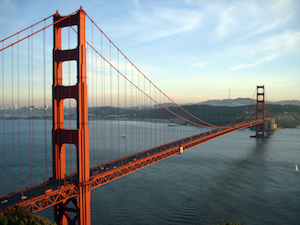
\includegraphics[width=\linewidth]{external/datafiles/golden-gate-bridge.png}
\end{image}%
This program changes every pixel of the image.%
\begin{program}{Python}{0}{1}{0}
import image

img = image.Image("golden_gate.png")
win = image.ImageWin(img.getWidth(), img.getHeight())
img.draw(win)

# img.setDelay(delay, number of pixels between delay)
# setDelay(1, 400) will speed up a lot
img.setDelay(1,15)

for row in range(img.getHeight()):
    for col in range(img.getWidth()):
        p = img.getPixel(col, row)

        newred = p.red * 1.4
        newgreen =  p.green * .75
        newblue =  p.blue * 1.1

        newpixel = image.Pixel(newred, newgreen, newblue)

        img.setPixel(col, row, newpixel)

img.draw(win)
win.exitonclick()
\end{program}
\end{computation}
The examples above all use Python, which will run in your browser.   Other languages will only run when a project is hosted on Runestone Academy servers.  And in this case there is a small twist.  You need to indicate which existing \mono{<datafile>} your program needs, even if that seems obvious by reading the code.  To do this, make sure each datafile has an \mono{@xml:id} and then use the \mono{@add-files} attribute on \mono{<program>} to specify a list of xml:id's that you want to be available.  These datafiles will be written to the program's working directory using the filename specified by the \mono{@filename} attribute of the \mono{<datafile>} element, and are the names you use in your program's code.  As before, no path information is needed, nor allowed.%
\par
When the \mono{@language} attribute of a \mono{<program>} is set to \mono{python3} that means in-browser Python is not good enough, and you want the greater power and flexibility of having your code run on a Runestone Academy server.  So this is our first example of using the \mono{@datafile} attribute.%
\par
The data file is an abbreviated version of the example above, just to be different.  And is not editable.%
\begin{preformatted}
Data: ccdata2.txt
\end{preformatted}
\begin{preformatted}
1900    -0.2      2.38
1910    -0.49     3.34
1920    -0.25     4.01
1930    -0.14     4.53
\end{preformatted}
The program is identical to the above, but we specify \mono{python3} as the language, and use the smaller file.  So this example is only active when this content is hosted on a Runestone Academy server.%
\begin{program}{Python}{0}{1}{0}
ccfile = open("ccdata2.txt", "r")

for aline in ccfile:
    values = aline.split()
    print('In', values[0], 'the average temp. was', values[1], '°C and CO2 emmisions were', values[2], 'gigatons.')

ccfile.close()
\end{program}
[2023-02-24 Testing Java with multiple data files]%
\begin{data}{Data}{Flowers.}{data-files-20}%
Two flower images as \mono{<datafile>} for use in upcoming Java program.%
\begin{preformatted}
Data: flower1.jpg
\end{preformatted}
\begin{image}{0.415}{0.17}{0.415}{}%

\includegraphics[width=\linewidth]{external/datafiles/flower-one.jpeg}
\end{image}%
\begin{preformatted}
Data: flower2.jpg
\end{preformatted}
\begin{image}{0.415}{0.17}{0.415}{}%
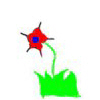
\includegraphics[width=\linewidth]{external/datafiles/flower-two.jpeg}
\end{image}%
\end{data}
\begin{program}{Java}{0}{1}{0}
import java.awt.*;
import java.awt.font.*;
import java.awt.geom.*;
import java.awt.image.BufferedImage;
import java.text.*;
import java.util.*;
import java.util.List;

/**
 * A class that represents a picture.  This class inherits from
 * SimplePicture and allows the student to add functionality to
 * the Picture class.
 *
 * @author Barbara Ericson ericson@cc.gatech.edu
 */
public class Picture extends SimplePicture
{
  ///////////////////// constructors //////////////////////////////////

  /**
   * Constructor that takes no arguments
   */
  public Picture ()
  {
    /* not needed but use it to show students the implicit call to super()
     * child constructors always call a parent constructor
     */
    super();
  }

  /**
   * Constructor that takes a file name and creates the picture
   * @param fileName the name of the file to create the picture from
   */
  public Picture(String fileName)
  {
    // let the parent class handle this fileName
    super(fileName);
  }

  /**
   * Constructor that takes the height and width
   * @param height the height of the desired picture
   * @param width the width of the desired picture
   */
  public Picture(int width, int height)
  {
    // let the parent class handle this width and height
    super(width,height);
  }

  /**
   * Constructor that takes a picture and creates a
   * copy of that picture
   * @param copyPicture the picture to copy
   */
  public Picture(Picture copyPicture)
  {
    // let the parent class do the copy
    super(copyPicture);
  }

  /**
   * Constructor that takes a buffered image
   * @param image the buffered image to use
   */
  public Picture(BufferedImage image)
  {
    super(image);
  }
  ////////////////////// methods ///////////////////////////////////////

  /**
   * Method to return a string with information about this picture.
   * @return a string with information about the picture such as fileName,
   * height and width.
   */
  public String toString()
  {
    String output = "Picture, filename " + getFileName() +
      " height " + getHeight()
      + " width " + getWidth();
    return output;
  }

  /**
    zeroBlue() method sets the blue values at all pixels to zero
 */
  public void zeroBlue()
  {
    Pixel[][] pixels = this.getPixels2D();

    for (Pixel[] rowArray : pixels)
     {
       for (Pixel p: rowArray)
       {
              p.setBlue(0);
       }
    }
  }

  /* mirrorVertical() */
  public void mirrorVertical()
  {
       Pixel[][] pixels = this.getPixels2D();
       Pixel leftPixel = null;
       Pixel rightPixel = null;
       int width = pixels[0].length;
       for (int row = 0; row < pixels.length; row++)
       {
            for (int col = 0; col < width / 2; col++)
            {
                 leftPixel = pixels[row][col];
                 rightPixel = pixels[row][width - 1 - col];
                 rightPixel.setColor(leftPixel.getColor());
            }
       }
  }

   /** copy from the passed fromPic to the
     * specified startRow and startCol in the
     * current picture
     * @param fromPic the picture to copy from
     * @param startRow the start row to copy to
     * @param startCol the start col to copy to
     */
   public void copy(Picture fromPic,
                  int startRow, int startCol)
   {
     Pixel fromPixel = null;
     Pixel toPixel = null;
     Pixel[][] toPixels = this.getPixels2D();
     Pixel[][] fromPixels = fromPic.getPixels2D();
     for (int fromRow = 0, toRow = startRow;
          fromRow < fromPixels.length &&
          toRow < toPixels.length;
          fromRow++, toRow++)
     {
       for (int fromCol = 0, toCol = startCol;
            fromCol < fromPixels[0].length &&
            toCol < toPixels[0].length;
            fromCol++, toCol++)
       {
         fromPixel = fromPixels[fromRow][fromCol];
         toPixel = toPixels[toRow][toCol];
         toPixel.setColor(fromPixel.getColor());
       }
     }
   }

  public void createCollage()
  {
       // You can also try butterfly.jpg and snowflake.jpg
       Picture flower1 = new Picture("flower1.jpg");
       Picture flower2 = new Picture("flower2.jpg");
       this.copy(flower1,0,0);
       this.copy(flower2,100,0);
       this.copy(flower1,200,0);
       Picture flowerNoBlue = new Picture(flower2);
       flowerNoBlue.zeroBlue();
       this.copy(flowerNoBlue,300,0);
       this.copy(flower1,400,0);
       this.copy(flower2,500,0);
       this.mirrorVertical();
       this.show();
  }

  /* Main method for testing
   */
  public static void main(String[] args)
  {
     Picture p = new Picture(500,500);
     p.createCollage();
  }
}
\end{program}
The following is experimental, as of 2023-07-05, and needs some organization, plus some credit to CSAwesome and Barb Ericson.%
\begin{preformatted}
Data: beach.jpg
\end{preformatted}
\begin{image}{0.415}{0.17}{0.415}{}%
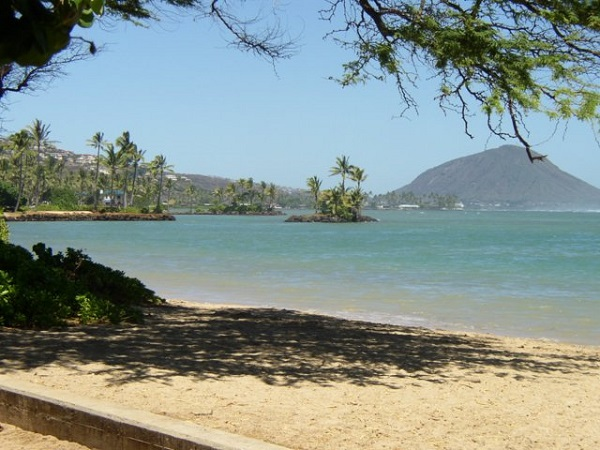
\includegraphics[width=\linewidth]{external/datafiles/beach.jpg}
\end{image}%
\begin{preformatted}
Data: pictureClasses1.jar
\end{preformatted}
\begin{preformatted}
import java.awt.Image;
import java.awt.image.BufferedImage;

/**
 * Interface to describe a digital picture.  A digital pict→
 * associated file name.  It can have a title.  It has pixe→
 * associated with it and you can get and set the pixels.  →
 * can get an Image from a picture or a BufferedImage.  You→
 * it from a file name or image.  You can show a picture.  →
 * explore a picture.  You can create a new image for it.
 *
 * @author Barb Ericson ericson@cc.gatech.edu
 */
public interface DigitalPicture
{
  public String getFileName(); // get the file name that th→
  public String getTitle(); // get the title of the picture
  public void setTitle(String title); // set the title of t→
  public int getWidth(); // get the width of the picture in→
  public int getHeight(); // get the height of the picture →
\end{preformatted}
\begin{program}{Java}{0}{1}{0}
import java.awt.*;
import java.awt.font.*;
import java.awt.geom.*;
import java.awt.image.BufferedImage;
import java.text.*;
import java.util.*;
import java.util.List;

/**
 * A class that represents a picture.  This class inherits from
 * SimplePicture and allows the student to add functionality to
 * the Picture class.
 *
 * @author Barbara Ericson ericson@cc.gatech.edu
 */
public class Picture extends SimplePicture
{
  ///////////////////// constructors //////////////////////////////////

  /**
   * Constructor that takes no arguments
   */
  public Picture ()
  {
    /* not needed but use it to show students the implicit call to super()
     * child constructors always call a parent constructor
     */
    super();
  }

  /**
   * Constructor that takes a file name and creates the picture
   * @param fileName the name of the file to create the picture from
   */
  public Picture(String fileName)
  {
    // let the parent class handle this fileName
    super(fileName);
  }

  /**
   * Constructor that takes the height and width
   * @param height the height of the desired picture
   * @param width the width of the desired picture
   */
  public Picture(int height, int width)
  {
    // let the parent class handle this width and height
    super(width,height);
  }

  /**
   * Constructor that takes a picture and creates a
   * copy of that picture
   * @param copyPicture the picture to copy
   */
  public Picture(Picture copyPicture)
  {
    // let the parent class do the copy
    super(copyPicture);
  }

  /**
   * Constructor that takes a buffered image
   * @param image the buffered image to use
   */
  public Picture(BufferedImage image)
  {
    super(image);
  }
  ////////////////////// methods ///////////////////////////////////////

  /**
   * Method to return a string with information about this picture.
   * @return a string with information about the picture such as fileName,
   * height and width.
   */
  public String toString()
  {
    String output = "Picture, filename " + getFileName() +
      " height " + getHeight()
      + " width " + getWidth();
    return output;

  }

  /**
    zeroBlue() method sets the blue values at all pixels to zero
 */
  public void zeroBlue()
  {
    Pixel[][] pixels = this.getPixels2D();

    for (Pixel[] rowArray : pixels)
     {
       for (Pixel p: rowArray)
       {
              p.setBlue(0);
       }
    }
  }


 /*
    keepOnlyBlue() method sets the blue values at all pixels to zero.

    Add new method here and call it from main.
 */

  /* Main method for testing
   */
  public static void main(String[] args)
  {
    Picture pict = new Picture("beach.jpg");
    pict.show();
    pict.zeroBlue(); // Change this to call keepOnlyBlue()
    pict.show();
  }
}
\end{program}
\end{sectionptx}
%
%
\typeout{************************************************}
\typeout{Section 5.6 YouTube Videos}
\typeout{************************************************}
%
\begin{sectionptx}{Section}{YouTube Videos}{}{YouTube Videos}{}{}{videos-in-runestone}
Runestone uses a YouTube API that broadcasts events when a reader interacts with a video.  In this way, Runestone can record video-watching as an activity.  As PreTeXt output we concede better behavior on small screens (``responsiveness'') to enable this feature in a Runestone version.  A \mono{@label} attribute is necessary for persistence in the Runestone database.  Various PreTeXt features, such as playlists, are not yet supported\textemdash{}make a request.%
\begin{sidebyside}{2}{0.075}{0.075}{0.17}%
\begin{sbspanel}{0.47}%
\noindent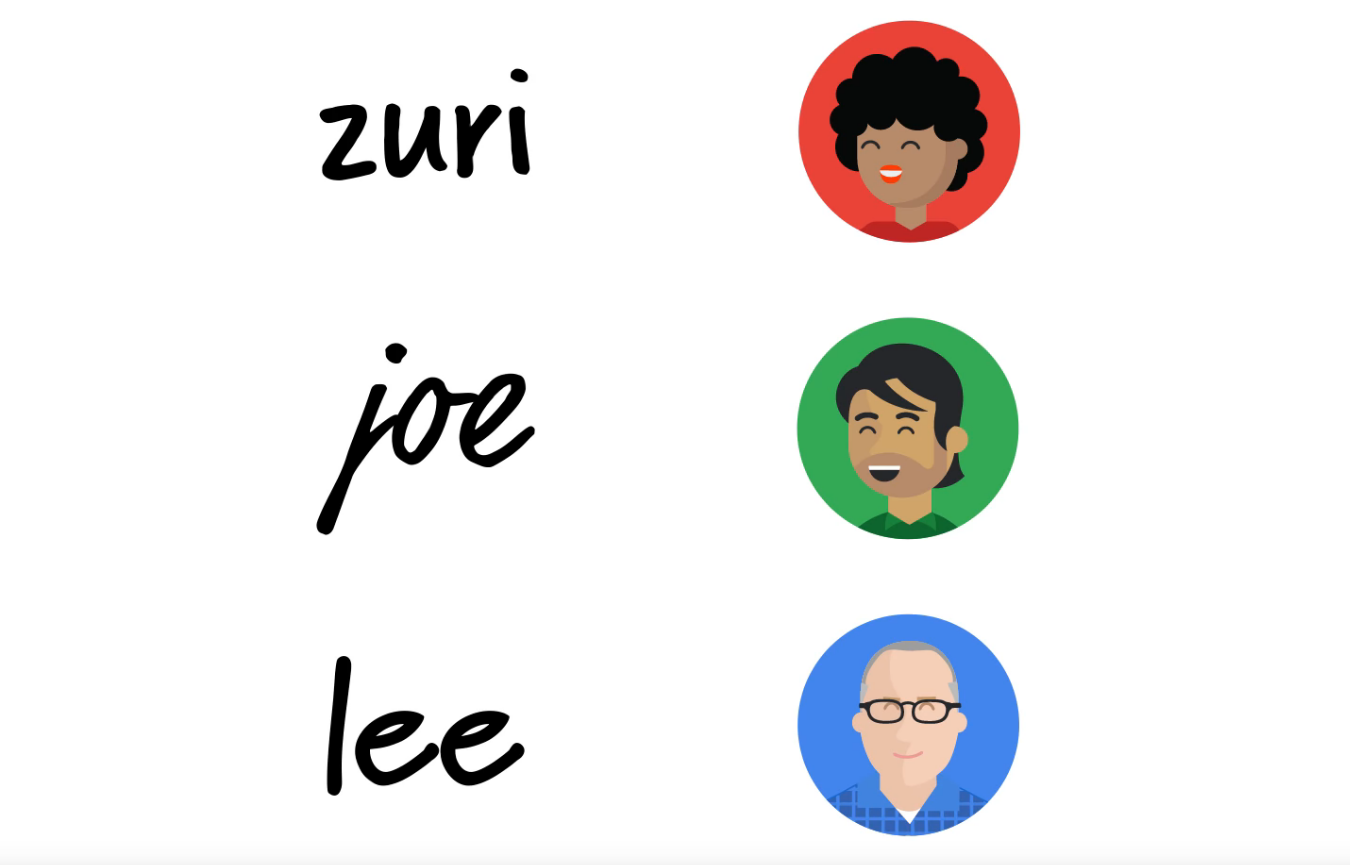
\includegraphics[width=\linewidth]{external/yt-list-variables.png}
\end{sbspanel}%
\begin{sbspanel}{0.21}%
\noindent
\includegraphics[width=\linewidth]{generated/qrcode/youtube-list-vars.png}
\href{https://pretextbook.org/examples/noparts/decorative/html/youtube-list-vars.html}{Standalone}%
\end{sbspanel}%
\end{sidebyside}%
\par
The margins here are asymmetric just as a test.  And this text is here to see where the video ends.%
\end{sectionptx}
%
%
\typeout{************************************************}
\typeout{Section 5.7 Deeper}
\typeout{************************************************}
%
\begin{sectionptx}{Section}{Deeper}{}{Deeper}{}{}{rune-nested-divisions}
\begin{introduction}{}%
This is a stub of a \mono{<section>}, but it contains two \mono{<subsection>} which each contain a PROJECT-LIKE item that includes a \mono{<program>} element, and thus is a coding exercise.  This tests migration to the Runestone assignment area, though Runestone only has divisions two-deep (``chapter'' and ``subchapter'', so both will show up associated with the same \mono{<section>}\textemdash{}this one.%
\par
The first is a start of a C program, so will only be interactive on a Runestone server.  The second is a Python program, so will be interactive in all HTML outputs.%
\end{introduction}%
%
%
\typeout{************************************************}
\typeout{Subsection 5.7.1 Subsection One}
\typeout{************************************************}
%
\begin{subsectionptx}{Subsection}{Subsection One}{}{Subsection One}{}{}{rune-nested-divisions-3}
An \mono{<activity>} next.  This one has a \mono{<program>} so will be made interactive whenever possible.%
\begin{activity}{Activity}{Activity in a Subsection.}{activity-in-subsection}%
We would suggest you do something here.%
\begin{program}{C}{0}{1}{0}
#include <stdio.h>

int main(void)
\end{program}
\end{activity}%
Nothing suggests this next \mono{<project>} is interactive.%
\begin{project}{Project}{Project in a Subsection.}{rune-nested-divisions-3-5}%
You would work this project on paper, most likely.  It is \emph{never} interactive since there is no indication of a desire for that, even if hosted on a capable platform.%
\par
A little bit of markup, to test a bug: \(x^2\).  (The bug was only apparent under a deprecated method for specify a question to be an interactive short-answer question on Runestone Academy.)%
\end{project}%
\end{subsectionptx}
%
%
\typeout{************************************************}
\typeout{Subsection 5.7.2 Subsection Two}
\typeout{************************************************}
%
\begin{subsectionptx}{Subsection}{Subsection Two}{}{Subsection Two}{}{}{rune-nested-divisions-4}
An \mono{<exploration>} next.%
\begin{exploration}{Exploration}{Exploration in a Subsection.}{exploration-with-always-static-program}%
We would suggest now that you explore something here.  In this case we simply provide a CodeLens, which would be graded as an ``interaction''.%
\begin{program}{Python}{0}{1}{0}
for i in range(10):
    print(i)
\end{program}
\end{exploration}%
The next simple \mono{<exercise>} will be a ``short answer'' question on a capable interactive platform since we have included a \mono{<response>} element.%
\begin{inlineexercise}{Checkpoint}{Inline Exercise in a Subsection.}{interactive-short-answer}%
I am an interactive short answer question, but only on a capable platform.%
\end{inlineexercise}%
\end{subsectionptx}
\end{sectionptx}
%
%
\typeout{************************************************}
\typeout{Exercises 5.8 True\slash{}False Exercises}
\typeout{************************************************}
%
\begin{exercises-section}{Exercises}{True\slash{}False Exercises}{}{True\slash{}False Exercises}{}{}{true-false-exercises}
\begin{divisionexercise}{1}{True\slash{}False.}{}{vector-space-dimension}%
\index{vector space}%
True or False?%
\par
Every vector space has finite dimension.%
\par\smallskip%
\noindent\textbf{\blocktitlefont Hint}.\hypertarget{vector-space-dimension-4}{}\quad{}\(P_n\), the vector space of polynomials with degree at most \(n\), has dimension \(n+1\) by \hyperref[theorem-exponent-laws]{Theorem~{\xreffont\ref{theorem-exponent-laws}}}.  [Cross-reference is just a demo, content is not relevant.]  What happens if we relax the defintion and remove the parameter \(n\)?%
\par\smallskip%
\noindent\textbf{\blocktitlefont Answer}.\hypertarget{vector-space-dimension-5}{}\quad{}False.%
\par\smallskip%
\noindent\textbf{\blocktitlefont Solution}.\hypertarget{vector-space-dimension-6}{}\quad{}False.%
\par
The vector space of all polynomials with finite degree has a basis, \(B = \{1,x,x^2,x^3,\dots\}\), which is infinte.%
\end{divisionexercise}%
\end{exercises-section}
%
%
\typeout{************************************************}
\typeout{Exercises 5.9 Multiple Choice Exercises}
\typeout{************************************************}
%
\begin{exercises-section}{Exercises}{Multiple Choice Exercises}{}{Multiple Choice Exercises}{}{}{exercises-groupwork}
\begin{introduction}{}%
When this \mono{<exercises>} division is hosted on Runestone Academy, it will be enabled for group work.  See group selection and submission features are at the end of the division.  See \hyperref[worksheet-groupwork]{Worksheet~{\xreffont\ref{worksheet-groupwork}}} for more detail.  (2024-07-24: experimental.)%
\end{introduction}%
\begin{divisionexercise}{1}{Multiple-Choice, Not Randomized, One Answer.}{}{multiple-choice-not-randomized}%
\index{stop signs}%
What color is a stop sign?%
\par
%
\begin{enumerate}[label={\Alph*.}]
\item{}Green%
\item{}Red%
\item{}White%
\end{enumerate}
%
\par\smallskip%
\noindent\textbf{\blocktitlefont Hint 1}.\hypertarget{multiple-choice-not-randomized-4}{}\quad{}What did you see last time you went driving?%
\par\smallskip%
\noindent\textbf{\blocktitlefont Hint 2}.\hypertarget{multiple-choice-not-randomized-5}{}\quad{}Maybe go out for a drive?%
\par\smallskip%
\noindent\textbf{\blocktitlefont Answer}.\hypertarget{multiple-choice-not-randomized-6}{}\quad{}B.%
\par\smallskip%
\noindent\textbf{\blocktitlefont Solution}.\hypertarget{multiple-choice-not-randomized-7}{}\quad{}%
\begin{enumerate}[label={\Alph*.}]
\item{}\lititle{Incorrect.}\par%
Green means ``go!''.%
\item{}\lititle{Correct.}\par%
Red is universally used for prohibited activities or serious warnings.%
\item{}\lititle{Incorrect.}\par%
White might be hard to see.%
\end{enumerate}
%
\end{divisionexercise}%
\begin{divisionexercise}{2}{Multiple-Choice, Math in Feedback.}{}{multiple-choice-feedback-math}%
What is the coefficient on \(x^4y^4\) in \((2x+5xy^2)^4\)?%
\par
%
\begin{enumerate}[label={\Alph*.}]
\item{}\(\displaystyle 6\)%
\item{}\(\displaystyle 60\)%
\item{}\(\displaystyle 100\)%
\item{}\(\displaystyle 600\)%
\end{enumerate}
%
\par\smallskip%
\noindent\textbf{\blocktitlefont Answer}.\hypertarget{multiple-choice-feedback-math-3}{}\quad{}D.%
\par\smallskip%
\noindent\textbf{\blocktitlefont Solution}.\hypertarget{multiple-choice-feedback-math-4}{}\quad{}%
\begin{enumerate}[label={\Alph*.}]
\item{}\lititle{Incorrect.}\par%
Have you accounted for the \(2\) and \(5\) that are in the original binomial?%
\item{}\lititle{Incorrect.}\par%
What should the exponents on \(2\) and \(5\) be when you expand \((2x+5xy^2)^4\)?%
\item{}\lititle{Incorrect.}\par%
Have you included something of the form \(\binom{n}{k}\) in your computations?%
\item{}\lititle{Correct.}\par%
Correct! Using the binomial theorem, we get a term containing the monomial \(x^4y^4\) by taking two of the first term, and two of the second term in the expansion of \((2x+5xy^2)^4\), and so this term is equal to%
\begin{equation*}
\binom{4}{2} (2x)^2 (5xy^2)^2 = 6 \cdot 2^2 5^2 x^4 y^4 = 600 x^4 y^4\text{.}
\end{equation*}
%
\end{enumerate}
%
\end{divisionexercise}%
\begin{divisionexercise}{3}{Multiple-Choice, Not Randomized, Multiple Answers.}{}{multiple-choice-multiple-answers}%
\index{stop signs}%
Which colors might be found in a rainbow?  (Note that the radio buttons now allow multiple buttons to be selected.)%
\par
%
\begin{enumerate}[label={\Alph*.}]
\item{}Red%
\item{}Yellow%
\item{}Black%
\item{}Green%
\end{enumerate}
%
\par\smallskip%
\noindent\textbf{\blocktitlefont Hint}.\hypertarget{multiple-choice-multiple-answers-4}{}\quad{}Do you know the acronym\textellipsis{}\acronym{ROY G BIV} for the colors of a rainbow, and their order?%
\par\smallskip%
\noindent\textbf{\blocktitlefont Answer}.\hypertarget{multiple-choice-multiple-answers-5}{}\quad{}A, B, D.%
\par\smallskip%
\noindent\textbf{\blocktitlefont Solution}.\hypertarget{multiple-choice-multiple-answers-6}{}\quad{}%
\begin{enumerate}[label={\Alph*.}]
\item{}\lititle{Correct.}\par%
Red is a definitely one of the colors.%
\item{}\lititle{Correct.}\par%
Yes, yellow is correct.%
\item{}\lititle{Incorrect.}\par%
Remember the acronym\textellipsis{}\acronym{ROY G BIV}.  ``B'' stands for blue.%
\item{}\lititle{Correct.}\par%
Yes, green is one of the colors.%
\end{enumerate}
%
\end{divisionexercise}%
\begin{divisionexercise}{4}{Multiple-Choice, Randomized, One Answer.}{}{multiple-choice-randomized}%
\index{stop signs}%
What color is a stop sign? [Static versions retain the order as authored.]%
\par
%
\begin{enumerate}[label={\Alph*.}]
\item{}Green%
\item{}Red%
\item{}White%
\end{enumerate}
%
\par\smallskip%
\noindent\textbf{\blocktitlefont Hint 1}.\hypertarget{multiple-choice-randomized-4}{}\quad{}What did you see last time you went driving?%
\par\smallskip%
\noindent\textbf{\blocktitlefont Hint 2}.\hypertarget{multiple-choice-randomized-5}{}\quad{}Maybe go out for a drive?%
\par\smallskip%
\noindent\textbf{\blocktitlefont Answer}.\hypertarget{multiple-choice-randomized-6}{}\quad{}B.%
\par\smallskip%
\noindent\textbf{\blocktitlefont Solution}.\hypertarget{multiple-choice-randomized-7}{}\quad{}%
\begin{enumerate}[label={\Alph*.}]
\item{}\lititle{Incorrect.}\par%
Green means ``go!''.%
\item{}\lititle{Correct.}\par%
Red is universally used for prohibited activities or serious warnings.%
\item{}\lititle{Incorrect.}\par%
White might be hard to see.%
\end{enumerate}
%
\end{divisionexercise}%
\begin{divisionexercise}{5}{Multiple-Choice, Randomized, One Answer but with Checkboxes.}{}{multiple-choice-randomized-forced-checkbox}%
\index{stop signs}%
What color is a stop sign? [Static versions retain the order as authored.]%
\par
%
\begin{enumerate}[label={\Alph*.}]
\item{}Green%
\item{}Red%
\item{}Yellow%
\end{enumerate}
%
\par\smallskip%
\noindent\textbf{\blocktitlefont Hint 1}.\hypertarget{multiple-choice-randomized-forced-checkbox-4}{}\quad{}What did you see last time you went driving?%
\par\smallskip%
\noindent\textbf{\blocktitlefont Hint 2}.\hypertarget{multiple-choice-randomized-forced-checkbox-5}{}\quad{}Maybe go out for a drive?%
\par\smallskip%
\noindent\textbf{\blocktitlefont Answer}.\hypertarget{multiple-choice-randomized-forced-checkbox-6}{}\quad{}B.%
\par\smallskip%
\noindent\textbf{\blocktitlefont Solution}.\hypertarget{multiple-choice-randomized-forced-checkbox-7}{}\quad{}%
\begin{enumerate}[label={\Alph*.}]
\item{}\lititle{Incorrect.}\par%
Green means ``go!''.%
\item{}\lititle{Correct.}\par%
Red is universally used for prohibited activities or serious warnings.%
\item{}\lititle{Incorrect.}\par%
Yellow means slow down.%
\end{enumerate}
%
\end{divisionexercise}%
\begin{divisionexercise}{6}{Multiple-Choice, Randomized, Multiple Answers.}{}{multiple-choice-randomized-multiple-answers}%
\index{stop signs}%
Which colors might be found in a rainbow?  (Note that the radio buttons now allow multiple buttons to be selected.) [Static versions retain the order as authored.]%
\par
%
\begin{enumerate}[label={\Alph*.}]
\item{}Red%
\item{}Yellow%
\item{}Black%
\item{}Green%
\end{enumerate}
%
\par\smallskip%
\noindent\textbf{\blocktitlefont Hint}.\hypertarget{multiple-choice-randomized-multiple-answers-4}{}\quad{}Do you know the acronym\textellipsis{}\acronym{ROY G BIV} for the colors of a rainbow, and their order?%
\par\smallskip%
\noindent\textbf{\blocktitlefont Answer}.\hypertarget{multiple-choice-randomized-multiple-answers-5}{}\quad{}A, B, D.%
\par\smallskip%
\noindent\textbf{\blocktitlefont Solution}.\hypertarget{multiple-choice-randomized-multiple-answers-6}{}\quad{}%
\begin{enumerate}[label={\Alph*.}]
\item{}\lititle{Correct.}\par%
Red is a definitely one of the colors.%
\item{}\lititle{Correct.}\par%
Yes, yellow is correct.%
\item{}\lititle{Incorrect.}\par%
Remember the acronym\textellipsis{}\acronym{ROY G BIV}.  ``B'' stands for blue.%
\item{}\lititle{Correct.}\par%
Yes, green is one of the colors.%
\end{enumerate}
%
\end{divisionexercise}%
\begin{divisionexercise}{7}{Mathematical Multiple-Choice, Not Randomized, Multiple Answers.}{}{mathematical-multiple-choice-multiple-answers}%
\index{stop signs}%
Which of the following is an antiderivative of \(2\sin(x)\cos(x)\)?%
\par
%
\begin{enumerate}[label={\Alph*.}]
\item{}\(\displaystyle \sin^2(x)+832\)%
\item{}\(\displaystyle \sin^2(x)\)%
\item{}\(\displaystyle -\cos^2(x)\)%
\item{}\(\displaystyle -2\cos(x)\sin(x)\)%
\end{enumerate}
%
\par\smallskip%
\noindent\textbf{\blocktitlefont Hint}.\hypertarget{mathematical-multiple-choice-multiple-answers-4}{}\quad{}You can take a derivative on any one of the choices to see if it is correct or not, rather than using techniques of integration to find \emph{a single} correct answer.%
\par\smallskip%
\noindent\textbf{\blocktitlefont Answer}.\hypertarget{mathematical-multiple-choice-multiple-answers-5}{}\quad{}A, B, C.%
\par\smallskip%
\noindent\textbf{\blocktitlefont Solution}.\hypertarget{mathematical-multiple-choice-multiple-answers-6}{}\quad{}%
\begin{enumerate}[label={\Alph*.}]
\item{}\lititle{Correct.}\par%
Remember that when we write \(+C\) on an antiderivative that this is the way we communicate that there are \emph{many} possible derivatives, but they all ``differ by a constant''.%
\item{}\lititle{Correct.}\par%
The derivative given in the statement of the problem looks exactly like an application of the chain rule to \(\sin^2(x)\).%
\item{}\lititle{Correct.}\par%
Take a derivative on \(-\cos^2(x)\) to see that this answer is correct.  Extra credit: does this answer ``differ by a constant'' when subtracted from either of the other two correct answers?%
\item{}\lititle{Incorrect.}\par%
The antiderivative of a product is not the product of the antiderivatives.  Use the product rule to take a derivative and see that this answer is not correct.%
\end{enumerate}
%
\end{divisionexercise}%
\begin{divisionexercise}{8}{Multiple-Choice, Not Randomized, One Answer.}{}{multiple-choice-columns}%
\index{stop signs}%
What color is a stop sign?%
\par
Note: we are experimenting with choices in columns (2025-05-17).  Three columns here.%
\par
%
\begin{multicols}{3}
\begin{enumerate}[label={\Alph*.}]
\item{}Green%
\item{}Red%
\item{}White%
\item{}Purple%
\item{}Pink%
\end{enumerate}
\end{multicols}
%
\par\smallskip%
\noindent\textbf{\blocktitlefont Hint 1}.\hypertarget{multiple-choice-columns-4}{}\quad{}What did you see last time you went driving?%
\par\smallskip%
\noindent\textbf{\blocktitlefont Hint 2}.\hypertarget{multiple-choice-columns-5}{}\quad{}Maybe go out for a drive?%
\par\smallskip%
\noindent\textbf{\blocktitlefont Answer}.\hypertarget{multiple-choice-columns-6}{}\quad{}B.%
\par\smallskip%
\noindent\textbf{\blocktitlefont Solution}.\hypertarget{multiple-choice-columns-7}{}\quad{}%
\begin{enumerate}[label={\Alph*.}]
\item{}\lititle{Incorrect.}\par%
Green means ``go!''.%
\item{}\lititle{Correct.}\par%
Red is universally used for prohibited activities or serious warnings.%
\item{}\lititle{Incorrect.}\par%
White might be hard to see.%
\item{}\lititle{Incorrect.}\par%
Hmmmmmmm.%
\item{}\lititle{Incorrect.}\par%
I have never seen a pink road sign!%
\end{enumerate}
%
\end{divisionexercise}%
\end{exercises-section}
%
%
\typeout{************************************************}
\typeout{Exercises 5.10 Parsons Exercises}
\typeout{************************************************}
%
\begin{exercises-section}{Exercises}{Parsons Exercises}{}{Parsons Exercises}{}{}{parsons-exercises}
\begin{divisionexercise}{1}{Parsons Problem, Mathematical Proof.}{}{number-theory-proof}%
\index{even numbers}%
Create a proof of the theorem: If \(n\) is an even number, then \(n\equiv 0\mod 2\).%
\par
[Ed. If you examine the source, you will also notice the \mono{<exercise>} lacks a \mono{@language} attribute. It is relying on the \mono{docinfo/parsons/@language} value that is in bookinfo.xml. If present, that attribute will be used for any Parsons that lack a \mono{@language}.]%
\par
%
\begin{itemize}[label=\textbullet]
\item{}Click the heels of your ruby slippers together three times.%
\item{}Suppose \(n\) is even.%
\item{}%
\begin{itemize}[label=]
\item{}Either:%
\par
Then \(n\) is a prime number.%
\item{}Or:%
\par
Then there exists an \(m\) so that \(n = 2m\).%
\item{}Or:%
\par
Then there exists an \(m\) so that \(n = 2m + 1\).%
\end{itemize}
%
\item{}Thus \(n\equiv 0\mod 2\).%
\item{}So \(n = 2m + 0\).%
\par
This is a superfluous second paragraph in this block.%
\item{}And a little bit of irrelevant multi-line math%
\begin{align*}
c^2&a^2+b^2\\
&x^2+y^2\text{.}
\end{align*}
%
\end{itemize}
%
\par\smallskip%
\noindent\textbf{\blocktitlefont Solution}.\hypertarget{number-theory-proof-4}{}\quad{}%
\begin{itemize}[label=\textbullet]
\item{}Suppose \(n\) is even.%
\item{}Then there exists an \(m\) so that \(n = 2m\).%
\item{}So \(n = 2m + 0\).%
\par
This is a superfluous second paragraph in this block.%
\item{}Thus \(n\equiv 0\mod 2\).%
\end{itemize}
%
\end{divisionexercise}%
\begin{divisionexercise}{2}{Parsons Problem, Partial Ordering.}{}{parsons-with-partial-order}%
Parsons problems can specify a partial ordering that allows for multiple valid solutions.%
\par
Try putting the blocks in a valid order to calculate and print\mono{c} Only use the required blocks. There are many valid orderings.%
\par
%
\begin{itemize}[label=\textbullet]
\item{}%
\begin{codedisplayleft}
c = math.sqrt(cSquared)
\end{codedisplayleft}
%
\item{}%
\begin{itemize}[label=]
\item{}Either:%
\par
%
\begin{codedisplay}
b = 4
\end{codedisplay}
%
\item{}Or:%
\par
%
\begin{codedisplay}
4 = b
\end{codedisplay}
%
\end{itemize}
%
\item{}%
\begin{codedisplayleft}
cSquared = a ** 2 + b ** 2
\end{codedisplayleft}
%
\item{}%
\begin{codedisplayleft}
print(c)
\end{codedisplayleft}
%
\item{}%
\begin{codedisplayleft}
import math
\end{codedisplayleft}
%
\item{}%
\begin{codedisplayleft}
a = 3
\end{codedisplayleft}
%
\item{}%
\begin{codedisplayleft}
import antigravity
\end{codedisplayleft}
%
\end{itemize}
%
\par\smallskip%
\noindent\textbf{\blocktitlefont Solution}.\hypertarget{parsons-with-partial-order-3}{}\quad{}\begin{program}{Python}{0}{1}{0}
import math
a = 3
b = 4
cSquared = a ** 2 + b ** 2
c = math.sqrt(cSquared)
print(c)
\end{program}
\end{divisionexercise}%
\begin{divisionexercise}{3}{Parsons Problem, Programming.}{}{prime-number-program-indent-yes}%
\index{prime numbers}%
\index{Sieve of Eratosthenes}%
The Sieve of Eratosthenes computes prime numbers by starting with a finite list of the integers bigger than 1.  The first member of the list is a prime and is saved\slash{}recorded.  Then all multiples of that prime (which not a prime, excepting the prime itself!) are removed from the list.  Now the first number remaining in the list is the next prime number.  And the process repeats.%
\par
The code blocks below can be rearranged to form one of the many possible programs to implement this algorithm to compute a list of all the primes less than \(250\). [Ed. this version of this problem requires the reader to provide the necessary indentation.]%
\par
This reprises \hyperlink{sieve-primes}{Exercise~{\xreffont 2.5.1}}.%
\par
%
\begin{itemize}[label=\textbullet]
\item{}%
\begin{codedisplayleft}
for nonprime in range(p, n, p):
\end{codedisplayleft}
%
\item{}%
\begin{itemize}[label=]
\item{}Either:%
\par
%
\begin{codedisplay}
primes = []
candidates = list(range(2,n))
\end{codedisplay}
%
\item{}Or:%
\par
%
\begin{codedisplay}
candidates = []
primes = list(range(2,n))
\end{codedisplay}
%
\end{itemize}
%
\item{}%
\begin{codedisplayleft}
p = candidates[0]
primes.append(p)
\end{codedisplayleft}
%
\item{}%
\begin{codedisplayleft}
print(primes)
\end{codedisplayleft}
%
\item{}%
\begin{codedisplayleft}
if nonprime in candidates:
    candidates.remove(nonprime)
\end{codedisplayleft}
%
\item{}%
\begin{codedisplayleft}
n = 250
\end{codedisplayleft}
%
\item{}%
\begin{codedisplayleft}
primes = candidates + [p]
\end{codedisplayleft}
%
\item{}%
\begin{codedisplayleft}
while candidates:
\end{codedisplayleft}
%
\end{itemize}
%
\par\smallskip%
\noindent\textbf{\blocktitlefont Solution}.\hypertarget{prime-number-program-indent-yes-5}{}\quad{}\begin{program}{Python}{0}{1}{0}
n = 250
primes = []
candidates = list(range(2,n))
while candidates:
    p = candidates[0]
    primes.append(p)
    for nonprime in range(p, n, p):
        if nonprime in candidates:
            candidates.remove(nonprime)
print(primes)
\end{program}
\end{divisionexercise}%
\begin{divisionexercise}{4}{Parsons Problem with executable.}{}{parsons-with-executable}%
Parsons problems that have a \mono{language} specified that corresponds to a valid activecode language can be made runnable.%
\par
Complete the Python function \mono{isolateRed(p)} If either the blue or green is higher than the red, average the three color values and set red, green, and blue to be that average. Otherwise, do nothing to \mono{p}.%
\par
After you check a correct answer you will be able to Run the code you created - it will be used to modify the image shown below.%
\begin{image}{0.25}{0.5}{0.25}{}%
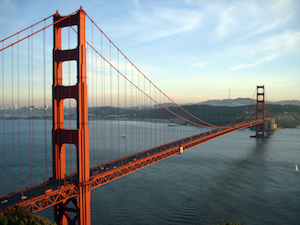
\includegraphics[width=\linewidth]{external/datafiles/golden-gate-bridge.png}
\end{image}%
%
\begin{itemize}[label=\textbullet]
\item{}%
\begin{codedisplayleft}[showspaces=true]
        p.red = avg
        p.blue = avg
        p.green = avg
\end{codedisplayleft}
%
\item{}%
\begin{codedisplayleft}[showspaces=true]
    if p.green > p.red or p.blue > p.red:
\end{codedisplayleft}
%
\item{}%
\begin{codedisplayleft}[showspaces=true]
        avg = (p.red + p.blue + p.green) / 3
\end{codedisplayleft}
%
\item{}%
\begin{codedisplayleft}[showspaces=true]
def isolateRed(p):
\end{codedisplayleft}
%
\end{itemize}
%
\par\smallskip%
\noindent\textbf{\blocktitlefont Solution}.\hypertarget{parsons-with-executable-3}{}\quad{}\begin{program}{Python}{0}{1}{0}
def isolateRed(p):
    if p.green > p.red or p.blue > p.red:
        avg = (p.red + p.blue + p.green) / 3
        p.red = avg
        p.blue = avg
        p.green = avg
\end{program}
\end{divisionexercise}%
\begin{divisionexercise}{5}{Parsons Problem, Programming.}{}{prime-number-program-indent-no}%
\index{prime numbers}%
\index{Sieve of Eratosthenes}%
The Sieve of Eratosthenes computes prime numbers by starting with a finite list of the integers bigger than 1.  The first member of the list is a prime and is saved\slash{}recorded.  Then all multiples of that prime (which not a prime, excepting the prime itself!) are removed from the list.  Now the first number remaining in the list is the next prime number.  And the process repeats.%
\par
The code blocks below can be rearranged to form one of the many possible programs to implement this algorithm to compute a list of all the primes less than \(250\). [Ed. this version of this problem does not require the reader to provide the necessary indentation, which is the default.]%
\par
This reprises \hyperlink{sieve-primes}{Exercise~{\xreffont 2.5.1}}.%
\par
%
\begin{itemize}[label=\textbullet]
\item{}%
\begin{codedisplayleft}[showspaces=true]
    for nonprime in range(p, n, p):
\end{codedisplayleft}
%
\item{}%
\begin{itemize}[label=]
\item{}Either:%
\par
%
\begin{codedisplay}
primes = []
candidates = list(range(2,n))
\end{codedisplay}
%
\item{}Or:%
\par
%
\begin{codedisplay}
candidates = []
primes = list(range(2,n))
\end{codedisplay}
%
\end{itemize}
%
\item{}%
\begin{codedisplayleft}[showspaces=true]
    p = candidates[0]
    primes.append(p)
\end{codedisplayleft}
%
\item{}%
\begin{codedisplayleft}[showspaces=true]
print(primes)
\end{codedisplayleft}
%
\item{}%
\begin{codedisplayleft}[showspaces=true]
        if nonprime in candidates:
            candidates.remove(nonprime)
\end{codedisplayleft}
%
\item{}%
\begin{codedisplayleft}[showspaces=true]
n = 250
\end{codedisplayleft}
%
\item{}%
\begin{codedisplayleft}[showspaces=true]
primes = candidates + [p]
\end{codedisplayleft}
%
\item{}%
\begin{codedisplayleft}[showspaces=true]
while candidates:
\end{codedisplayleft}
%
\end{itemize}
%
\par\smallskip%
\noindent\textbf{\blocktitlefont Solution}.\hypertarget{prime-number-program-indent-no-5}{}\quad{}\begin{program}{Python}{0}{1}{0}
n = 250
primes = []
candidates = list(range(2,n))
while candidates:
    p = candidates[0]
    primes.append(p)
    for nonprime in range(p, n, p):
        if nonprime in candidates:
            candidates.remove(nonprime)
print(primes)
\end{program}
\end{divisionexercise}%
\begin{divisionexercise}{6}{Parsons Problem, Mathematical Proof, Numbered Blocks.}{}{number-theory-proof-numbered-left}%
\index{even numbers}%
Create a proof of the theorem: If \(n\) is an even number, then \(n\equiv 0\mod 2\). [Ed.  This version has numbered blocks, online they are on the right end of the block.]%
\par
%
\begin{enumerate}[label={\arabic*.}]
\item{}Click the heels of your ruby slippers together three times.%
\item{}Suppose \(n\) is even.%
\item{}%
\begin{enumerate}[label={(\alph*)}]
\item{}Then \(n\) is a prime number.%
\item{}Then there exists an \(m\) so that \(n = 2m\).%
\item{}Then there exists an \(m\) so that \(n = 2m + 1\).%
\end{enumerate}
%
\item{}Thus \(n\equiv 0\mod 2\).%
\item{}So \(n = 2m + 0\).%
\par
This is a superfluous second paragraph in this block.%
\end{enumerate}
%
\par\smallskip%
\noindent\textbf{\blocktitlefont Answer}.\hypertarget{number-theory-proof-numbered-left-4}{}\quad{}2, 3b, 5, 4%
\par\smallskip%
\noindent\textbf{\blocktitlefont Solution}.\hypertarget{number-theory-proof-numbered-left-5}{}\quad{}%
\begin{descriptionlist}
\begin{dlinarrow}{2}{number-theory-proof-numbered-left-5-1-1-1}%
Suppose \(n\) is even.%
\end{dlinarrow}%
\begin{dlinarrow}{3b}{number-theory-proof-numbered-left-5-1-1-2}%
Then there exists an \(m\) so that \(n = 2m\).%
\end{dlinarrow}%
\begin{dlinarrow}{5}{number-theory-proof-numbered-left-5-1-1-3}%
So \(n = 2m + 0\).%
\par
This is a superfluous second paragraph in this block.%
\end{dlinarrow}%
\begin{dlinarrow}{4}{number-theory-proof-numbered-left-5-1-1-4}%
Thus \(n\equiv 0\mod 2\).%
\end{dlinarrow}%
\end{descriptionlist}
%
\end{divisionexercise}%
\begin{divisionexercise}{7}{Parsons Problem, Programming.}{}{prime-number-program-numbered-right}%
\index{prime numbers}%
\index{Sieve of Eratosthenes}%
The Sieve of Eratosthenes computes prime numbers by starting with a finite list of the integers bigger than 1.  The first member of the list is a prime and is saved\slash{}recorded.  Then all multiples of that prime (which not a prime, excepting the prime itself!) are removed from the list.  Now the first number remaining in the list is the next prime number.  And the process repeats.%
\par
The code blocks below can be rearranged to form one of the many possible programs to implement this algorithm to compute a list of all the primes less than \(250\). [Ed.  This version has numbered blocks, online they are on the left end of the block.]%
\par
This reprises \hyperlink{sieve-primes}{Exercise~{\xreffont 2.5.1}}.%
\par
%
\begin{enumerate}[label={\arabic*.}]
\item{}%
\begin{codedisplayleft}
for nonprime in range(p, n, p):
\end{codedisplayleft}
%
\item{}%
\begin{enumerate}[label={(\alph*)}]
\item{}%
\begin{codedisplay}
primes = []
candidates = list(range(2,n))
\end{codedisplay}
%
\item{}%
\begin{codedisplay}
candidates = []
primes = list(range(2,n))
\end{codedisplay}
%
\end{enumerate}
%
\item{}%
\begin{codedisplayleft}
p = candidates[0]
primes.append(p)
\end{codedisplayleft}
%
\item{}%
\begin{codedisplayleft}
print(primes)
\end{codedisplayleft}
%
\item{}%
\begin{codedisplayleft}
if nonprime in candidates:
    candidates.remove(nonprime)
\end{codedisplayleft}
%
\item{}%
\begin{codedisplayleft}
n = 250
\end{codedisplayleft}
%
\item{}%
\begin{codedisplayleft}
primes = candidates + [p]
\end{codedisplayleft}
%
\item{}%
\begin{codedisplayleft}
while candidates:
\end{codedisplayleft}
%
\end{enumerate}
%
\par\smallskip%
\noindent\textbf{\blocktitlefont Answer}.\hypertarget{prime-number-program-numbered-right-5}{}\quad{}6, 2a, 8, 3, 1, 5, 4%
\par\smallskip%
\noindent\textbf{\blocktitlefont Solution}.\hypertarget{prime-number-program-numbered-right-6}{}\quad{}\begin{program}{Python}{0}{1}{0}
n = 250
primes = []
candidates = list(range(2,n))
while candidates:
    p = candidates[0]
    primes.append(p)
    for nonprime in range(p, n, p):
        if nonprime in candidates:
            candidates.remove(nonprime)
print(primes)
\end{program}
\end{divisionexercise}%
\end{exercises-section}
%
%
\typeout{************************************************}
\typeout{Exercises 5.11 Horizontal Parsons Exercises}
\typeout{************************************************}
%
\begin{exercises-section}{Exercises}{Horizontal Parsons Exercises}{}{Horizontal Parsons Exercises}{}{}{horizontal-parsons-exercises}
\begin{divisionexercise}{1}{Parsons Problem, SQL statement.}{}{horizontal-parson-sql-statement-simple}%
Form the SQL statement by rearranging the four blocks.%
\par
%
\begin{codedisplay}
 | * | SELECT | test | FROM | 
\end{codedisplay}
%
\par\smallskip%
\noindent\textbf{\blocktitlefont Solution}.\hypertarget{horizontal-parson-sql-statement-simple-3}{}\quad{}%
\begin{codedisplay}
SELECT * FROM test
\end{codedisplay}
%
\end{divisionexercise}%
\begin{divisionexercise}{2}{Parsons Problem, Python import.}{}{horizontal-parson-python-test}%
This is testing that horizontal parsons get the default programming language from \mono{docinfo/parsons/@language}.%
\par
%
\begin{codedisplay}
 | math | from | pi | import | 
\end{codedisplay}
%
\par\smallskip%
\noindent\textbf{\blocktitlefont Solution}.\hypertarget{horizontal-parson-python-test-3}{}\quad{}%
\begin{codedisplay}
from math import pi
\end{codedisplay}
%
\end{divisionexercise}%
\begin{divisionexercise}{3}{Parsons Problem, SQL statement, no randomization.}{}{horizontal-parson-sql-statement-no-randomize}%
Form the SQL statement by rearranging the four blocks.  This version of this problem will \emph{always} present the blocks in the same fixed order (but incorrect, hopefully!), as prescribed by the author in the source.%
\par
%
\begin{codedisplay}
 | * | SELECT | test | FROM | 
\end{codedisplay}
%
\par\smallskip%
\noindent\textbf{\blocktitlefont Solution}.\hypertarget{horizontal-parson-sql-statement-no-randomize-3}{}\quad{}%
\begin{codedisplay}
SELECT * FROM test
\end{codedisplay}
%
\end{divisionexercise}%
\begin{divisionexercise}{4}{Parsons Problem, SQL statement, automatic feedback.}{}{horizontal-parson-sql-statement-with-db}%
Form the SQL statement by rearranging the four blocks.%
\par
%
\begin{codedisplay}
 | * | SELECT | test | FROM | 
\end{codedisplay}
%
\par\smallskip%
\noindent\textbf{\blocktitlefont Solution}.\hypertarget{horizontal-parson-sql-statement-with-db-3}{}\quad{}%
\begin{codedisplay}
SELECT * FROM test
\end{codedisplay}
%
\end{divisionexercise}%
\begin{divisionexercise}{5}{Parsons Problem, Natural Language.}{}{horizontal-parson-natural}%
Form the sentence often used to show font samples.  You can reuse blocks as needed.%
\par
%
\begin{codedisplay}
 | jumped | brown | fox | dog | over | the | lazy | quick | 
\end{codedisplay}
%
\par\smallskip%
\noindent\textbf{\blocktitlefont Solution}.\hypertarget{horizontal-parson-natural-3}{}\quad{}%
\begin{codedisplay}
the quick brown fox jumped over the lazy dog
\end{codedisplay}
%
\end{divisionexercise}%
\begin{divisionexercise}{6}{Parsons Problem, Natural Language, with Distractors.}{}{horizontal-parson-natural-distractor}%
Form the sentence often used to show font samples.  Again, but now with distractors.%
\par
%
\begin{codedisplay}
 | jumped | quick | brown | fox | dog | bar | over | the | foo | lazy | 
\end{codedisplay}
%
\par\smallskip%
\noindent\textbf{\blocktitlefont Solution}.\hypertarget{horizontal-parson-natural-distractor-3}{}\quad{}%
\begin{codedisplay}
the quick brown fox jumped over the lazy dog
\end{codedisplay}
%
\end{divisionexercise}%
\begin{divisionexercise}{7}{Parsons Problem, SQL statement, reusable.}{}{horizontal-parson-sql-statement-reusable}%
Form the SQL statement by rearranging the four blocks.  Same problem as above, but we allow blocks to be reused (even though the solution does not require that).%
\par
%
\begin{codedisplay}
 | * | SELECT | test | FROM | 
\end{codedisplay}
%
\par\smallskip%
\noindent\textbf{\blocktitlefont Solution}.\hypertarget{horizontal-parson-sql-statement-reusable-3}{}\quad{}%
\begin{codedisplay}
SELECT * FROM test
\end{codedisplay}
%
\end{divisionexercise}%
\end{exercises-section}
%
%
\typeout{************************************************}
\typeout{Exercises 5.12 Matching Exercises}
\typeout{************************************************}
%
\begin{exercises-section}{Exercises}{Matching Exercises}{}{Matching Exercises}{}{}{matching-exercises}
\begin{introduction}{}%
Matching exercises come in two varieties. Their differences are most noticeable in interactive versions.%
\begin{descriptionlist}
\begin{dlimedium}{Cardsort}{matching-exercises-2-1-1-1}%
A \mono{<cardsort>} asks users to match items in a 1-1 or many-1 fashion. The interactive version of these involves dragging ``card''s from the left column (the \mono{<premise>}s) into containers on the right (the \mono{<response>}s).%
\end{dlimedium}%
\begin{dlimedium}{Matching}{matching-exercises-2-1-1-2}%
A \mono{<matching>} interactive asks users to form connections between the \mono{<premise>}s in the left column and the \mono{<response>}s on the right. This format supports many-many matches.%
\end{dlimedium}%
\end{descriptionlist}
%
\end{introduction}%
\begin{divisionexercise}{1}{Cardsort Problem, Dates.}{}{matching-dates}%
\index{matching US dates}%
Match each event in United States history with the year it happened.%
\begin{center}%
{\tabularfont%
\begin{tabular}{lll}
Louisiana Purchase&~~&1823\tabularnewline\crulethin{1-1}\crulethin{3-3}
Battle of Gettysburg&~~&1886\tabularnewline\crulethin{1-1}\crulethin{3-3}
Haymarket Riot&~~&1803\tabularnewline\crulethin{1-1}\crulethin{3-3}
Monroe Doctrine&~~&1863
\end{tabular}
}%
\end{center}%
\par\smallskip%
\noindent\textbf{\blocktitlefont Solution}.\hypertarget{matching-dates-4}{}\quad{}%
\begin{itemize}[label=\textbullet]
\item{}1823%
\begin{itemize}[label=$\circ$]
\item{}Monroe Doctrine%
\end{itemize}
%
\item{}1886%
\begin{itemize}[label=$\circ$]
\item{}Haymarket Riot%
\end{itemize}
%
\item{}1803%
\begin{itemize}[label=$\circ$]
\item{}Louisiana Purchase%
\end{itemize}
%
\item{}1863%
\begin{itemize}[label=$\circ$]
\item{}Battle of Gettysburg%
\end{itemize}
%
\end{itemize}
%
\end{divisionexercise}%
\begin{divisionexercise}{2}{Cardsort Problem, Derivatives.}{}{matching-derivatives}%
\index{matching derivatives}%
Match each function with its derivative.%
\begin{center}%
{\tabularfont%
\begin{tabular}{lll}
\(x^3-6x^2+5\)&~~&\(3x^2-12x\)\tabularnewline\crulethin{1-1}\crulethin{3-3}
\((x+1)^2\)&~~&\(-3x^{-4}\)\tabularnewline\crulethin{1-1}\crulethin{3-3}
\(x^{-3}\)&~~&\(2x+2\)
\end{tabular}
}%
\end{center}%
\par\smallskip%
\noindent\textbf{\blocktitlefont Solution}.\hypertarget{matching-derivatives-4}{}\quad{}%
\begin{itemize}[label=\textbullet]
\item{}\(3x^2-12x\)%
\begin{itemize}[label=$\circ$]
\item{}\(x^3-6x^2+5\)%
\end{itemize}
%
\item{}\(-3x^{-4}\)%
\begin{itemize}[label=$\circ$]
\item{}\(x^{-3}\)%
\end{itemize}
%
\item{}\(2x+2\)%
\begin{itemize}[label=$\circ$]
\item{}\((x+1)^2\)%
\end{itemize}
%
\end{itemize}
%
\end{divisionexercise}%
\begin{divisionexercise}{3}{Cardsort Problem, Linear Algebra.}{}{matching-bases}%
\index{matching bases and subspaces}%
Match each subspace with a basis for that subspace. (You may assume that each set is really a basis for at least one of the subspaces.)%
\begin{center}%
{\tabularfont%
\begin{tabular}{lll}
\(\left\{\langle x,y,z\rangle\mid - y + z = 0\right\}\)&~~&\(\left\{\langle -4, 3, 3\rangle, \langle 3, -2, -2 \rangle\right\}\)\tabularnewline\crulethin{1-1}\crulethin{3-3}
\(\left\{\langle x,y,z\rangle\mid -2x - 5y + 2z = 0\right\}\)&~~&\(\left\{\langle -4, 3, 3\rangle, \langle 5, -4, -5 \rangle\right\}\)\tabularnewline\crulethin{1-1}\crulethin{3-3}
\(\left\{\langle x,y,z\rangle\mid -3x - 5y + z = 0\right\}\)&~~&\(\left\{\langle 3, -2, -2 \rangle, \langle 5, -4, -5 \rangle\right\}\)
\end{tabular}
}%
\end{center}%
\par\smallskip%
\noindent\textbf{\blocktitlefont Hint}.\hypertarget{matching-bases-4}{}\quad{}For openers, a basis for a subspace must be a \emph{subset} of the subspace.%
\par\smallskip%
\noindent\textbf{\blocktitlefont Solution}.\hypertarget{matching-bases-5}{}\quad{}%
\begin{itemize}[label=\textbullet]
\item{}\(\left\{\langle -4, 3, 3\rangle, \langle 3, -2, -2 \rangle\right\}\)%
\begin{itemize}[label=$\circ$]
\item{}\(\left\{\langle x,y,z\rangle\mid - y + z = 0\right\}\)%
\end{itemize}
%
\item{}\(\left\{\langle -4, 3, 3\rangle, \langle 5, -4, -5 \rangle\right\}\)%
\begin{itemize}[label=$\circ$]
\item{}\(\left\{\langle x,y,z\rangle\mid -3x - 5y + z = 0\right\}\)%
\end{itemize}
%
\item{}\(\left\{\langle 3, -2, -2 \rangle, \langle 5, -4, -5 \rangle\right\}\)%
\begin{itemize}[label=$\circ$]
\item{}\(\left\{\langle x,y,z\rangle\mid -2x - 5y + 2z = 0\right\}\)%
\end{itemize}
%
\end{itemize}
%
\end{divisionexercise}%
\begin{divisionexercise}{4}{Cardsort Problem, Function Types.}{}{matching-function-types}%
\index{matching function types}%
Sort the following functions into their correct categories.%
\begin{center}%
{\tabularfont%
\begin{tabular}{lll}
\(y=2^x\)&~~&Linear\tabularnewline\crulethin{1-1}\crulethin{3-3}
\(y=x^3\)&~~&Quadratic\tabularnewline\crulethin{1-1}\crulethin{3-3}
\(y=\sqrt{x}\)&~~&Exponential\tabularnewline\crulethin{1-1}\crulethin{3-3}
\(y=5x+3\)&~~&Power\tabularnewline\crulethin{1-1}
\(\pi x - 6y = \sqrt{2}\)&~~&\tabularnewline\crulethin{1-1}
\(y=\frac{-1}{2}x+e\)&~~&\tabularnewline\crulethin{1-1}
\(y=x^3-x\)&~~&
\end{tabular}
}%
\end{center}%
\par\smallskip%
\noindent\textbf{\blocktitlefont Solution}.\hypertarget{matching-function-types-4}{}\quad{}%
\begin{itemize}[label=\textbullet]
\item{}Linear%
\begin{itemize}[label=$\circ$]
\item{}\(y=5x+3\)%
\item{}\(\pi x - 6y = \sqrt{2}\)%
\item{}\(y=\frac{-1}{2}x+e\)%
\end{itemize}
%
\item{}Quadratic%
\item{}(uncategorized)%
\begin{itemize}[label=$\circ$]
\item{}\(y=x^3-x\)%
\end{itemize}
%
\item{}Exponential%
\begin{itemize}[label=$\circ$]
\item{}\(y=2^x\)%
\end{itemize}
%
\item{}Power%
\begin{itemize}[label=$\circ$]
\item{}\(y=x^3\)%
\item{}\(y=\sqrt{x}\)%
\end{itemize}
%
\end{itemize}
%
\end{divisionexercise}%
\begin{divisionexercise}{5}{Matching Problem, Playing Cards.}{}{matching-playing-cards}%
\index{matching!playing cards}%
Associate each playing card with every applicable property.%
\begin{center}%
{\tabularfont%
\begin{tabular}{lll}
Jack of Hearts&~~&Spade\tabularnewline\crulethin{1-1}\crulethin{3-3}
Ace of Spades&~~&Club\tabularnewline\crulethin{1-1}\crulethin{3-3}
Queen of Spades&~~&Diamond\tabularnewline\crulethin{1-1}\crulethin{3-3}
King of Clubs&~~&Heart\tabularnewline\crulethin{1-1}\crulethin{3-3}
Queen of Diamonds&~~&Jack\tabularnewline\crulethin{3-3}
&~~&Queen\tabularnewline\crulethin{3-3}
&~~&King\tabularnewline\crulethin{3-3}
&~~&Ace
\end{tabular}
}%
\end{center}%
\par\smallskip%
\noindent\textbf{\blocktitlefont Solution}.\hypertarget{matching-playing-cards-4}{}\quad{}%
\begin{itemize}[label=\textbullet]
\item{}Ace%
\begin{itemize}[label=$\circ$]
\item{}Ace of Spades%
\end{itemize}
%
\item{}King%
\begin{itemize}[label=$\circ$]
\item{}King of Clubs%
\end{itemize}
%
\item{}Queen%
\begin{itemize}[label=$\circ$]
\item{}Queen of Spades%
\item{}Queen of Diamonds%
\end{itemize}
%
\item{}Jack%
\begin{itemize}[label=$\circ$]
\item{}Jack of Hearts%
\end{itemize}
%
\item{}Heart%
\begin{itemize}[label=$\circ$]
\item{}Jack of Hearts%
\end{itemize}
%
\item{}Diamond%
\begin{itemize}[label=$\circ$]
\item{}Queen of Diamonds%
\end{itemize}
%
\item{}Club%
\begin{itemize}[label=$\circ$]
\item{}King of Clubs%
\end{itemize}
%
\item{}Spade%
\begin{itemize}[label=$\circ$]
\item{}Ace of Spades%
\item{}Queen of Spades%
\end{itemize}
%
\end{itemize}
%
\end{divisionexercise}%
\begin{divisionexercise}{6}{Matching Problem, Popular Music History.}{}{matching-music-history}%
\index{matching music history}%
Drag each performer onto every applicable category.%
\begin{center}%
{\tabularfont%
\begin{tabular}{lll}
Paul&~~&Beatle\tabularnewline\crulethin{1-1}\crulethin{3-3}
Ringo&~~&Yardbirds\tabularnewline\crulethin{1-1}\crulethin{3-3}
Eric&~~&Guitarist\tabularnewline\crulethin{1-1}\crulethin{3-3}
Elton&~~&Drummer\tabularnewline\crulethin{1-1}\crulethin{3-3}
Jethro&~~&Flautist\tabularnewline\crulethin{3-3}
&~~&Harpist\tabularnewline\crulethin{3-3}
&~~&Pianist\tabularnewline\crulethin{3-3}
&~~&\emph{Some} "Math": \(\sin(x^2)\)
\end{tabular}
}%
\end{center}%
\par\smallskip%
\noindent\textbf{\blocktitlefont Solution}.\hypertarget{matching-music-history-4}{}\quad{}%
\begin{itemize}[label=\textbullet]
\item{}Beatle%
\begin{itemize}[label=$\circ$]
\item{}Paul%
\item{}Ringo%
\end{itemize}
%
\item{}Yardbirds%
\begin{itemize}[label=$\circ$]
\item{}Eric%
\end{itemize}
%
\item{}Guitarist%
\begin{itemize}[label=$\circ$]
\item{}Eric%
\end{itemize}
%
\item{}Drummer%
\begin{itemize}[label=$\circ$]
\item{}Ringo%
\end{itemize}
%
\item{}Flautist%
\item{}Harpist%
\item{}Pianist%
\begin{itemize}[label=$\circ$]
\item{}Elton%
\end{itemize}
%
\item{}\emph{Some} "Math": \(\sin(x^2)\)%
\item{}(uncategorized)%
\begin{itemize}[label=$\circ$]
\item{}Jethro%
\end{itemize}
%
\end{itemize}
%
\end{divisionexercise}%
\begin{divisionexercise}{7}{Cardsort Problem, Basic Arithmetic.}{}{cardsort-basic}%
\index{matching US dates}%
This is a simple exercise to test some grading behavior.%
\begin{center}%
{\tabularfont%
\begin{tabular}{lll}
2 + 3&~~&5\tabularnewline\crulethin{1-1}\crulethin{3-3}
\(12 + 2\)&~~&14\tabularnewline\crulethin{1-1}
4 + 1&~~&
\end{tabular}
}%
\end{center}%
\par\smallskip%
\noindent\textbf{\blocktitlefont Solution}.\hypertarget{cardsort-basic-4}{}\quad{}%
\begin{itemize}[label=\textbullet]
\item{}5%
\begin{itemize}[label=$\circ$]
\item{}2 + 3%
\item{}4 + 1%
\end{itemize}
%
\item{}14%
\begin{itemize}[label=$\circ$]
\item{}\(12 + 2\)%
\end{itemize}
%
\end{itemize}
%
\end{divisionexercise}%
\end{exercises-section}
%
%
\typeout{************************************************}
\typeout{Exercises 5.13 Clickable Area Exercises}
\typeout{************************************************}
%
\begin{exercises-section}{Exercises}{Clickable Area Exercises}{}{Clickable Area Exercises}{}{}{clickable-area-exercises}
\begin{divisionexercise}{1}{Clickable Areas, ``Regular'' Text.}{}{clickable-text}%
Identify (by clicking, or by circling) all of the nouns in this quotation by Eleanor Roosevelt.%
\par
``The future belongs to those who believe in the beauty of their dreams.''%
\par\smallskip%
\noindent\textbf{\blocktitlefont Answer}.\hypertarget{clickable-text-3}{}\quad{}Correct: \emph{future}; \emph{beauty}; \emph{dreams}. Incorrect: \deleted{those}; \deleted{their}.%
\par
The incorrect words are pronouns.%
\par\smallskip%
\noindent\textbf{\blocktitlefont Solution}.\hypertarget{clickable-text-4}{}\quad{}``The \emph{future} belongs to \deleted{those} who believe in the \emph{beauty} of \deleted{their} \emph{dreams}.''%
\end{divisionexercise}%
\begin{divisionexercise}{2}{Clickable Areas, Code.}{}{clickable-code}%
Identify (by clicking, or by circling) all of the assignment statements in this Python function.%
\begin{program}{none}{0}{1}{0}
def main():
    x = 4
    for i in range(5):
        y = i
        if y > 2:
            print(y)
\end{program}
\par\smallskip%
\noindent\textbf{\blocktitlefont Answer}.\hypertarget{clickable-code-3}{}\quad{}Correct: \mono{x = 4}; \mono{y = i}. Incorrect: \mono{def main():}; \mono{if y > 2:}.%
\par
Remember, the operator \mono{=} is used for assignment.%
\end{divisionexercise}%
\begin{divisionexercise}{3}{Clickable Areas, Text in a Table.}{}{clickable-table}%
A two-dimensional array was created in Python with the list comprehension:%
\begin{codedisplay}
[[0 for x in range(3)] for y in range(2)]
\end{codedisplay}
Then the values were (mostly) changed from zeros and the final array is shown below.%
\par
Identify (by clicking, or by circling) all of the boolean values in the array.%
\begin{center}%
{\tabularfont%
\begin{tabular}{AlAlAlA}\hrulethin
\mono{42}&\mono{True}&\mono{\textquotesingle{}towel\textquotesingle{}}\tabularnewline\hrulethin
\mono{\textquotesingle{}true\textquotesingle{}}&\mono{0}&\mono{False}\tabularnewline\hrulethin
\end{tabular}
}%
\end{center}%
This second table has no \mono{<area>}, in order to test CSS for tables.%
\begin{center}%
{\tabularfont%
\begin{tabular}{AlAlAlA}\hrulethin
\mono{42}&\mono{True}&\mono{\textquotesingle{}towel\textquotesingle{}}\tabularnewline\hrulethin
\mono{\textquotesingle{}true\textquotesingle{}}&\mono{0}&\mono{False}\tabularnewline\hrulethin
\end{tabular}
}%
\end{center}%
\par\smallskip%
\noindent\textbf{\blocktitlefont Hint}.\hypertarget{clickable-table-3}{}\quad{}Python boolean variables begin with capital latters.%
\par\smallskip%
\noindent\textbf{\blocktitlefont Answer}.\hypertarget{clickable-table-4}{}\quad{}Correct: \emph{\mono{True}}; \emph{\mono{False}}. Incorrect: \deleted{\mono{\textquotesingle{}towel\textquotesingle{}}}; \deleted{\mono{\textquotesingle{}true\textquotesingle{}}}.%
\par
Python boolean variables are \mono{True} and \mono{False}.  A value in quotation marks is a string, not a boolean.%
\par\smallskip%
\noindent\textbf{\blocktitlefont Solution}.\hypertarget{clickable-table-5}{}\quad{}\begin{center}%
{\tabularfont%
\begin{tabular}{AlAlAlA}\hrulethin
\mono{42}&\emph{\mono{True}}&\deleted{\mono{\textquotesingle{}towel\textquotesingle{}}}\tabularnewline\hrulethin
\deleted{\mono{\textquotesingle{}true\textquotesingle{}}}&\mono{0}&\emph{\mono{False}}\tabularnewline\hrulethin
\end{tabular}
}%
\end{center}%
This second table has no \mono{<area>}, in order to test CSS for tables.%
\begin{center}%
{\tabularfont%
\begin{tabular}{AlAlAlA}\hrulethin
\mono{42}&\mono{True}&\mono{\textquotesingle{}towel\textquotesingle{}}\tabularnewline\hrulethin
\mono{\textquotesingle{}true\textquotesingle{}}&\mono{0}&\mono{False}\tabularnewline\hrulethin
\end{tabular}
}%
\end{center}%
\end{divisionexercise}%
\end{exercises-section}
%
%
\typeout{************************************************}
\typeout{Exercises 5.14 Select Exercises}
\typeout{************************************************}
%
\begin{exercises-section}{Exercises}{Select Exercises}{}{Select Exercises}{}{}{select-exercises}
\begin{introduction}{}%
These \terminology{select} questions specify a list of extant questions, and the reader, or Runestone, selects questions from the list to be graded (in different ways). They are only really functional with a database of students in a course, i.e.~when hosted on Runestone.%
\end{introduction}%
\begin{divisionexercise}{1}{Three-way Select Question.}{}{question-select}%
Runestone-only: exercise to grade will be automatically chosen by Runestone from \hyperlink{vector-space-dimension}{Exercise~{\xreffont 5.8.1}}, \hyperlink{multiple-choice-not-randomized}{Exercise~{\xreffont 5.9.1}}, or \hyperlink{matching-dates}{Exercise~{\xreffont 5.12.1}}.%
\end{divisionexercise}%
\begin{divisionexercise}{2}{A\slash{}B Experiment Select Question.}{}{ab-experiment}%
Runestone-only: an A\slash{}B experiment (named \mono{sample-book}) with \hyperlink{vector-space-dimension}{Exercise~{\xreffont 5.8.1}} as (A) and \hyperlink{multiple-choice-not-randomized}{Exercise~{\xreffont 5.9.1}} as (B).%
\end{divisionexercise}%
\begin{divisionexercise}{3}{Grade First Question.}{}{toggle-first}%
Runestone-only: a toggle question where the question graded is \emph{always} the first of \hyperlink{vector-space-dimension}{Exercise~{\xreffont 5.8.1}}, or \hyperlink{multiple-choice-not-randomized}{Exercise~{\xreffont 5.9.1}}.%
\end{divisionexercise}%
\begin{divisionexercise}{4}{Grade Any Question.}{}{toggle-any}%
Runestone-only: a toggle question where the question graded is \emph{any} question chosen by the reader from \hyperlink{vector-space-dimension}{Exercise~{\xreffont 5.8.1}}, or \hyperlink{multiple-choice-not-randomized}{Exercise~{\xreffont 5.9.1}}.%
\end{divisionexercise}%
\end{exercises-section}
%
%
\typeout{************************************************}
\typeout{Exercises 5.15 Short Answer Exercises}
\typeout{************************************************}
%
\begin{exercises-section}{Exercises}{Short Answer Exercises}{}{Short Answer Exercises}{}{}{short-answer-exercises}
\begin{divisionexercise}{1}{Short Answer.}{}{short-answer-question}%
This sample book is configured to make some simple questions interactive on a capable platform, by adding a \mono{<response>} element as a signal.%
\end{divisionexercise}%
\end{exercises-section}
%
%
\typeout{************************************************}
\typeout{Section 5.16 Polling}
\typeout{************************************************}
%
\begin{sectionptx}{Section}{Polling}{}{Polling}{}{}{polling}
(2024-04-24) This section is experimental, and may not be fully functional as you view it.  No markup in the source document is final and may change at any time.%
\par
We begin with standalone queries, using the \mono{<query>} element.  Runestone calls these \terminology{polls}.   We plan structures\slash{}blocks such as \mono{<poll>}, \mono{<survey>}, and \mono{<questionnaire>}, that will be structured collections of \mono{<query>}.%
\begin{paragraphs}{Query.}{polling-4}%
In my town, the stoplights have:%
\par
%
\begin{enumerate}
\item{}Solid yellow lights.%
%
\item{}Yellow lights that are solid left-turn arrows.%
%
\item{}Yellow lights that are blinking left-turn arrows.%
%
\end{enumerate}
%
\end{paragraphs}%
\begin{paragraphs}{Query.}{polling-5}%
Which of the following is the derivative of \(f(x)=x^4\sin(x)\)?%
\par
%
\begin{enumerate}
\item{}\(x^5 - \cos(x)\)%
%
\item{}\(x^4\cos(x) + 4x^3\sin(x)\)%
%
\item{}\(4x^3\cos(x)\)%
%
\end{enumerate}
%
\end{paragraphs}%
\begin{paragraphs}{Query.}{polling-6}%
I like computer science better than mathematics.  ``1'' is ``strongly disagree'' and ``5'' is ``strongly agree''.%
\begin{preformatted}
1  2  3  4  5
\end{preformatted}
\end{paragraphs}%
\begin{paragraphs}{Query.}{polling-7}%
How many stuffed animal toys did you own growing up?  (Testing an absurdly large scale, especially in print.)%
\begin{preformatted}
1  2  3  4  5  6  7  8  9  10

11  12  13  14  15  16  17  18  19  20

21  22  23  24  25  26  27  28  29  30

31  32  33  34  35  36  37
\end{preformatted}
\end{paragraphs}%
\begin{paragraphs}{Query.}{polling-8}%
Which of the following paintings is your favorite?%
\par
%
\begin{enumerate}
\item{}  The Calydonian Boar Hunt by Peter Paul Rubens%
 \begin{image}{0.25}{0.5}{0.25}{}%
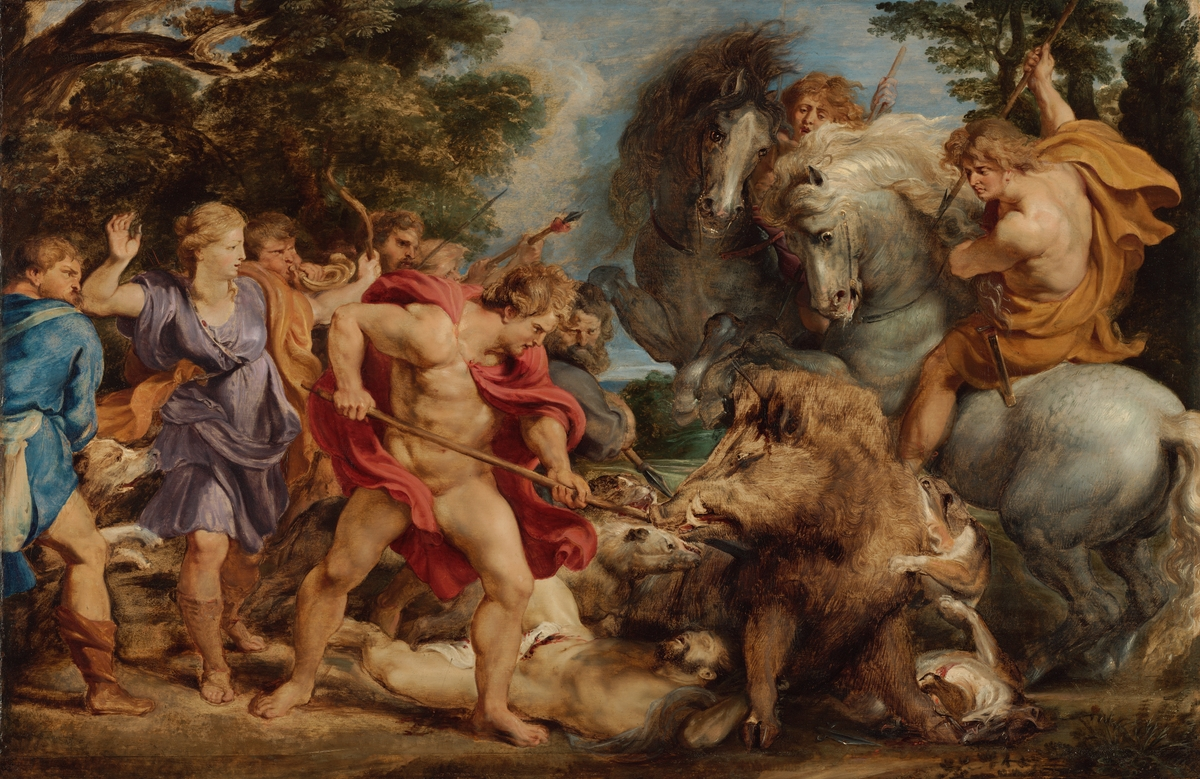
\includegraphics[width=\linewidth]{external/image-from-rawpixel-id-14263399-jpeg.jpg}
\end{image}%
%
\item{}  Lucas Cranach's The fountain of youth (1546)%
 \begin{image}{0.25}{0.5}{0.25}{}%
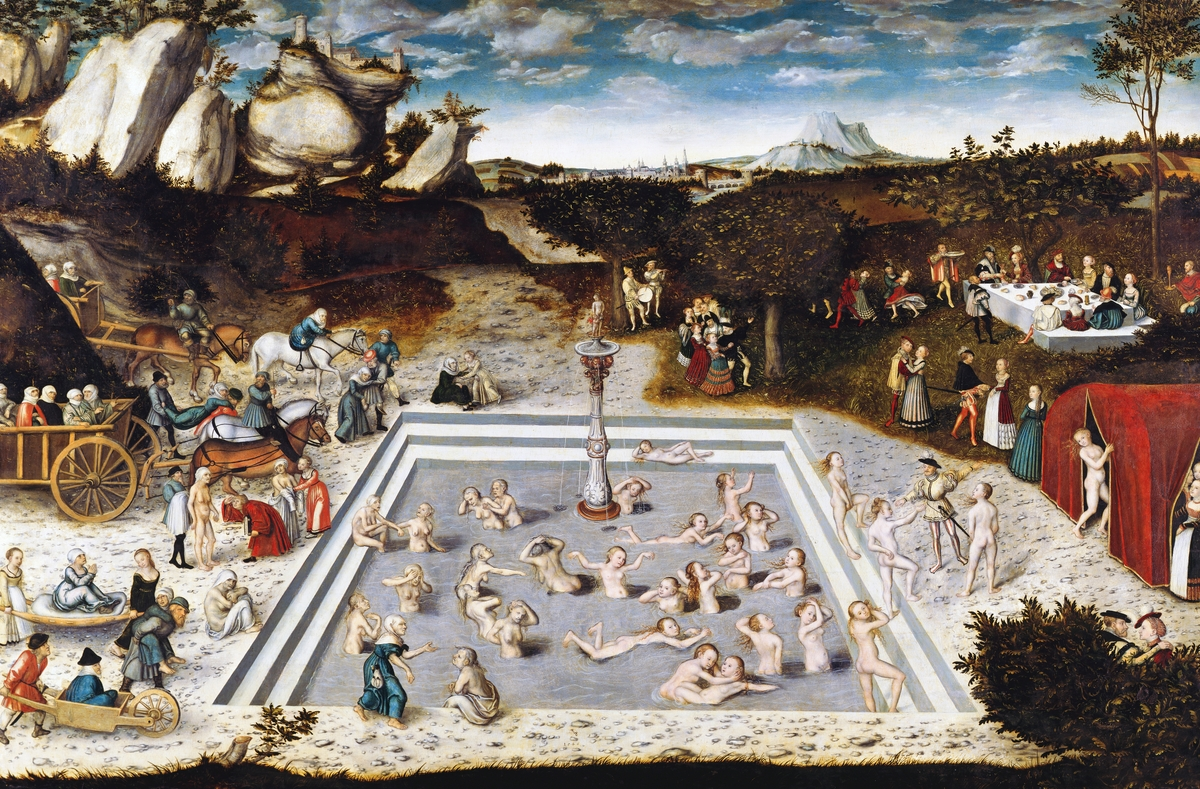
\includegraphics[width=\linewidth]{external/image-from-rawpixel-id-3984423-jpeg.jpg}
\end{image}%
%
\item{}  William-Adolphe Bouguereau's Temptation (1880)%
 \begin{image}{0.25}{0.5}{0.25}{}%
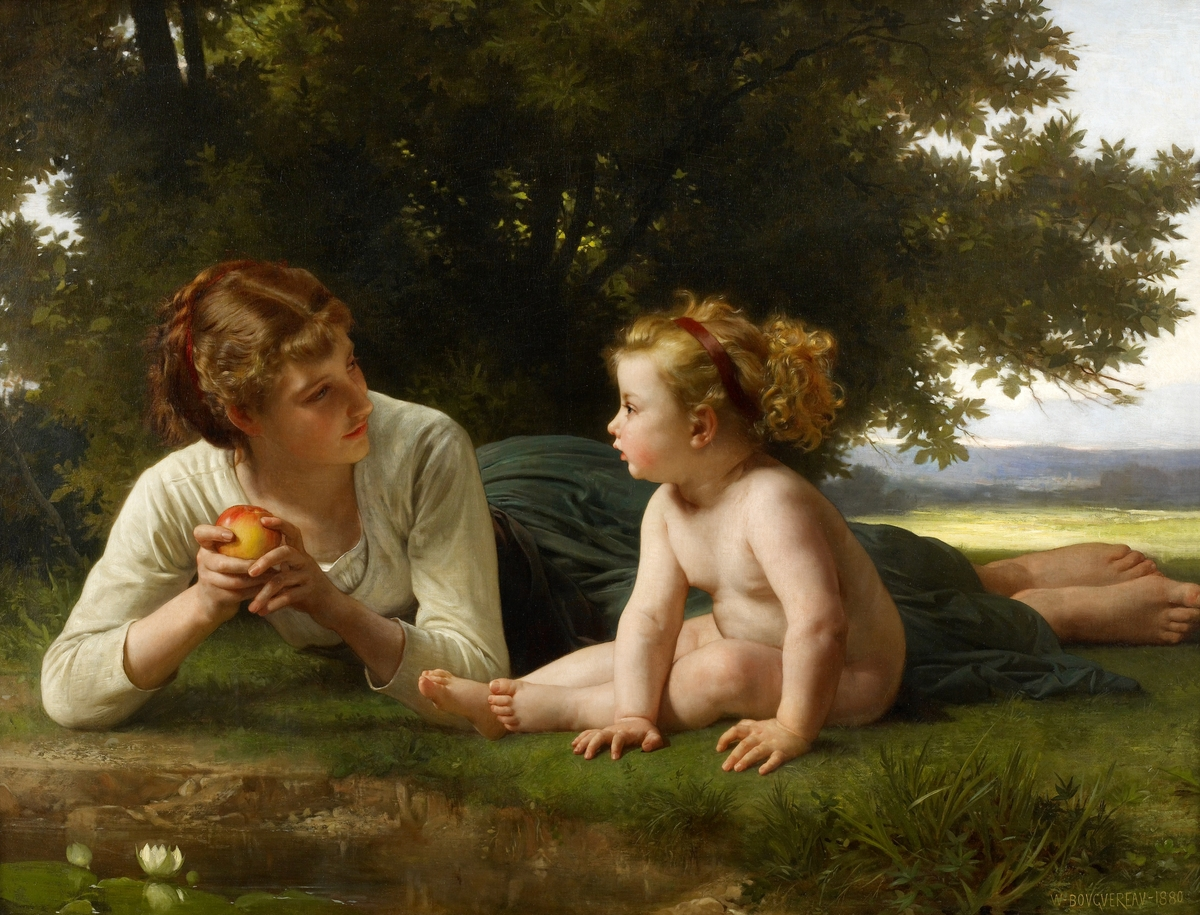
\includegraphics[width=\linewidth]{external/image-from-rawpixel-id-8704110-jpeg.jpg}
\end{image}%
%
\end{enumerate}
%
\end{paragraphs}%
\end{sectionptx}
%
%
\typeout{************************************************}
\typeout{Section 5.17 DoenetML}
\typeout{************************************************}
%
\begin{sectionptx}{Section}{DoenetML}{}{DoenetML}{}{}{doenet}
This preliminary DoenetML example is for testing use on a Runestone server, where it will use the SPLICE protocol to report out events.  To the reader, it should \emph{behave} identically when not on a Runestone server.%
\begin{sidebyside}{2}{0.075}{0.075}{0.17}%
\begin{sbspanel}{0.47}%
\noindent
\includegraphics[width=\linewidth]{generated/preview/interactive-doenetml-example-preview.png}
\end{sbspanel}%
\begin{sbspanel}{0.21}%
\noindent
\includegraphics[width=\linewidth]{generated/qrcode/interactive-doenetml-example.png}
\href{https://pretextbook.org/examples/noparts/decorative/html/interactive-doenetml-example.html}{Standalone}%
\par
\href{https://pretextbook.org/examples/noparts/decorative/html/interactive-doenetml-example-if.html}{Embed}%
\end{sbspanel}%
\end{sidebyside}%
\end{sectionptx}
%
%
\typeout{************************************************}
\typeout{Exercises 5.18 Fill-In Exercises (Old Style)}
\typeout{************************************************}
%
\begin{exercises-section}{Exercises}{Fill-In Exercises (Old Style)}{}{Fill-In Exercises (Old Style)}{}{}{fill-in-exercises-old}
\begin{introduction}{}%
This section has \terminology{fill-in-the-blank} (\initialism{FITB}) exercises that use an old syntax.  They were designed for projects transitioning from Runestone's ReST syntax to PreTeXt.  So they are really only here for testing, and not for any sort of documentation.  They will not receive support or enhancements.  \textit{Caveat emptor}.%
\end{introduction}%
\begin{divisionexercise}{1}{Fill-In, Integer Answer.}{}{fillin-integer}%
The game of bowling uses \fillintext{28} pins that you try to knock down. (This answer blank has been set to be very wide.)%
\par\smallskip%
\noindent\textbf{\blocktitlefont Solution}.\hypertarget{fillin-integer-3}{}\quad{}The game of bowling uses \fillintext{1}\(10\)\fillintext{1} pins that you try to knock down. (This answer blank has been set to be very wide.)%
\par
Arranged in a triangle, there are \(1+2+3+4 = 10\) pins, a so-called \terminology{triangular} number.%
\end{divisionexercise}%
\begin{divisionexercise}{2}{Fill-In, String and Number Answers.}{}{fillin-string-integer}%
Complete the following line of a Python program so that it will declare an integer variable \mono{age} with an initial value of \mono{5}. (These two answer blanks have been set to be very short.)%
\par
\fillintext{2} \mono{age = } \fillintext{3}\mono{;}%
\par\smallskip%
\noindent\textbf{\blocktitlefont Solution}.\hypertarget{fillin-string-integer-3}{}\quad{}Complete the following line of a Python program so that it will declare an integer variable \mono{age} with an initial value of \mono{5}. (These two answer blanks have been set to be very short.)%
\par
\fillintext{1}int\fillintext{1} \mono{age = } \fillintext{1}\(5\)\fillintext{1}\mono{;}%
\par
A variable of type \mono{int} is appropriate for whole number ages.%
\par
An integer variable may be initialized to a value.%
\end{divisionexercise}%
\begin{divisionexercise}{3}{Fill-In, Case-Insensitive Answer.}{}{fillin-case-insensitive}%
The word \fillintext{5} is the opposite of ``yes''.  (Try a mixture of upper and lower-case letters.)%
\par\smallskip%
\noindent\textbf{\blocktitlefont Solution}.\hypertarget{fillin-case-insensitive-3}{}\quad{}The word \fillintext{1}no\fillintext{1} is the opposite of ``yes''.  (Try a mixture of upper and lower-case letters.)%
\end{divisionexercise}%
\begin{divisionexercise}{4}{Fill-In, Decimal Answer.}{}{fillin-decimal}%
The decimal number \fillintext{5} is an approximation of \(\sfrac{1}{3}\) to within three significant figures.  (\href{https://en.wikipedia.org/wiki/Significant_figures}{Wikipedia}\footnotemark{}).%
\par\smallskip%
\noindent\textbf{\blocktitlefont Solution}.\hypertarget{fillin-decimal-3}{}\quad{}The decimal number \fillintext{1}\(0.333\)\fillintext{1} is an approximation of \(\sfrac{1}{3}\) to within three significant figures.  (\href{https://en.wikipedia.org/wiki/Significant_figures}{Wikipedia}\footnotemark{}).%
\par
Any value in the interval \(0.333\pm 0.0005\) is correct.%
\end{divisionexercise}%
\footnotetext[1]{\nolinkurl{en.wikipedia.org/wiki/Significant_figures}\label{fillin-decimal-2-1-4}}%
\footnotetext[2]{\nolinkurl{en.wikipedia.org/wiki/Significant_figures}\label{fillin-decimal-3-1-6}}%
\end{exercises-section}
%
%
\typeout{************************************************}
\typeout{Exercises 5.19 Fill-In Exercises}
\typeout{************************************************}
%
\begin{exercises-section}{Exercises}{Fill-In Exercises}{}{Fill-In Exercises}{}{}{fill-in-exercises}
\begin{introduction}{}%
This section has \terminology{fill-in-the-blank} (\initialism{FITB}) exercises using newer syntax, and the subject of active development.%
\end{introduction}%
\begin{divisionexercise}{1}{Fill-In, New Markup Numbers.}{}{fillin-numbers-many-tests}%
I love \(\pi\). What number am I thinking of, accurate to two decimal places?%
\par
\fillintext{5}%
\par\smallskip%
\noindent\textbf{\blocktitlefont Solution}.\hypertarget{fillin-numbers-many-tests-3}{}\quad{}I love \(\pi\). What number am I thinking of, accurate to two decimal places?%
\par
\fillintext{1}3.14\fillintext{1}%
\par
The decimal approximation of \(\pi\) is \(3.1415926535\ldots\), but to two decimal places we write \(3.14\).%
\end{divisionexercise}%
\begin{divisionexercise}{2}{Fill-In, New Markup Strings.}{}{fillin-strings-}%
The word I'm thinking about is hinted at by the image.%
\par
\begin{image}{0.25}{0.5}{0.25}{}%

\includegraphics[width=\linewidth]{external/cartoon-magic.jpg}
\end{image}%
%
\par
What word am I thinking about? \fillintext{5} (Interactive feedback explores a variety of options: Try what happens if you mix the case, or type in a number, or include more than the word, or try ``pizzazz''.")%
\par\smallskip%
\noindent\textbf{\blocktitlefont Hint}.\hypertarget{fillin-strings--3}{}\quad{}Do you really need a hint? Carefully reread the question.%
\par\smallskip%
\noindent\textbf{\blocktitlefont Solution}.\hypertarget{fillin-strings--4}{}\quad{}The word I'm thinking about is hinted at by the image.%
\par
\begin{image}{0.25}{0.5}{0.25}{}%

\includegraphics[width=\linewidth]{external/cartoon-magic.jpg}
\end{image}%
%
\par
What word am I thinking about? \fillintext{1}magic\fillintext{1} (Interactive feedback explores a variety of options: Try what happens if you mix the case, or type in a number, or include more than the word, or try ``pizzazz''.")%
\end{divisionexercise}%
\begin{divisionexercise}{3}{Fill-In, Javascript test of numbers.}{}{ex-demo-jscmp-primes}%
What is an example of a prime number less than 20? \fillintext{5}%
\par\smallskip%
\noindent\textbf{\blocktitlefont Solution}.\hypertarget{ex-demo-jscmp-primes-3}{}\quad{}What is an example of a prime number less than 20? \fillintext{1}13\fillintext{1}%
\par
Any number from the list \(\{2, 3, 5, 7, 11, 13, 17, 19\}\) is a prime number less than 20.%
\end{divisionexercise}%
\begin{divisionexercise}{4}{Fill-In, Javascript test of strings.}{}{fillin-jscmp-palindrome}%
What is an example of a palindrome? \fillintext{5}%
\par\smallskip%
\noindent\textbf{\blocktitlefont Solution}.\hypertarget{fillin-jscmp-palindrome-3}{}\quad{}What is an example of a palindrome? \fillintext{1}radar\fillintext{1}%
\par
Any word that is the same forward and backward is a palindrome.%
\end{divisionexercise}%
\begin{divisionexercise}{5}{Fill-In, Simple Randomization with Numbers.}{}{fillin-random-simple}%
What is the square of \(x=7\)? \(x^2=\)\fillintext{5}%
\par\smallskip%
\noindent\textbf{\blocktitlefont Solution}.\hypertarget{fillin-random-simple-3}{}\quad{}What is the square of \(x=7\)? \(x^2=\)\fillintext{1}\(49\)\fillintext{1}%
\end{divisionexercise}%
\begin{divisionexercise}{6}{Fill-In, Dynamic Math with Simple Numerical Answer.}{}{fillin-math-solve-equation}%
Solve the equation%
\begin{equation*}
-2 x-6=0
\end{equation*}
to get the value of \(x\).%
\par
\(x = \) \fillintext{5}%
\par\smallskip%
\noindent\textbf{\blocktitlefont Solution 1}.\hypertarget{fillin-math-solve-equation-3}{}\quad{}Solve the equation%
\begin{equation*}
-2 x-6=0
\end{equation*}
to get the value of \(x\).%
\par
\(x = \) \fillintext{1}\(-3\)\fillintext{1}%
\par\smallskip%
\noindent\textbf{\blocktitlefont Solution 2}.\hypertarget{fillin-math-solve-equation-4}{}\quad{}We want to isolate the \(x\) in the equation \(-2 x-6=0\). Because addition of \(-6\) is the last operation, we apply the inverse by adding \(6\) to both sides. The new, but equivalent equation is now \(-2x = 6\). Dividing both sides of the equation by \(-2\), we obtain the solution \(x=-3\).%
\end{divisionexercise}%
\begin{divisionexercise}{7}{Fill-In, Dynamic Math with Formulas as Answers.}{}{fillin-math-find-derivatives}%
Consider the function \(f(x)=-1 x^{5}-10\). Find \(f'(x)\) and \(f''(x)\).%
\par
\(f'(x) = \) \fillintext{15} and \(f''(x)=\) \fillintext{15}%
\par\smallskip%
\noindent\textbf{\blocktitlefont Solution 1}.\hypertarget{fillin-math-find-derivatives-3}{}\quad{}Consider the function \(f(x)=-1 x^{5}-10\). Find \(f'(x)\) and \(f''(x)\).%
\par
\(f'(x) = \) \fillintext{1}\(-\left(5 x^{4}\right)\)\fillintext{1} and \(f''(x)=\) \fillintext{1}\(-\left(20 x^{3}\right)\)\fillintext{1}%
\par\smallskip%
\noindent\textbf{\blocktitlefont Solution 2}.\hypertarget{fillin-math-find-derivatives-4}{}\quad{}The derivative of a constant is zero, so \(\frac{d}{dx}[-10]=0\). The term \(x^{5}\) is a power, so the power rule gives us \(\frac{d}{dx}[x^{5}]=5x^{4}\). Putting this together, we find \(f'(x)=-\left(5 x^{4}\right)\). Applying the power rule a second time, we find \(f''(x)=-\left(20 x^{3}\right)\).%
\end{divisionexercise}%
\begin{divisionexercise}{8}{Fill-In, Dynamic Math with Interdependent Formula Checking.}{}{fillin-math-decompose-function}%
Consider the function%
\begin{equation*}
h(x)=4 \left(-x-3\right)^{3}+5\text{.}
\end{equation*}
Find two nontrivial functions \(f(x)\) and \(g(x)\) so that \(h(x) = f(g(x))\).%
\par
\(f(x) = \) \fillintext{15} and \(g(x)=\) \fillintext{15}%
\par\smallskip%
\noindent\textbf{\blocktitlefont Solution 1}.\hypertarget{fillin-math-decompose-function-3}{}\quad{}Consider the function%
\begin{equation*}
h(x)=4 \left(-x-3\right)^{3}+5\text{.}
\end{equation*}
Find two nontrivial functions \(f(x)\) and \(g(x)\) so that \(h(x) = f(g(x))\).%
\par
\(f(x) = \) \fillintext{1}\(4 x^{3}+5\)\fillintext{1} and \(g(x)=\) \fillintext{1}\(-x-3\)\fillintext{1}%
\par\smallskip%
\noindent\textbf{\blocktitlefont Solution 2}.\hypertarget{fillin-math-decompose-function-4}{}\quad{}Noticing that the expression \(-x-3\) appears inside parentheses with a power, it makes sense to think of that as the inner function, defining \(g(x) = -x-3\). The outer function describes what happens to that. If we imagined replacing the formula \(-x-3\) with a box and then call that box our variable \(x\), we find the outer function is given by \(f(x) = 4 x^{3}+5\).%
\par
This is not the only non-trivial composition. Can you find others?%
\end{divisionexercise}%
\end{exercises-section}
%
%
\typeout{************************************************}
\typeout{Exercises 5.20 Hodgepodge}
\typeout{************************************************}
%
\begin{exercises-section}{Exercises}{Hodgepodge}{}{Hodgepodge}{}{}{runestone-hodgepodge}
\begin{divisionexercise}{1}{}{}{multifile-program-2}%
This is a test of accessing program resources across pages by relying on what is in the database.%
\begin{program}{C++}{0}{1}{0}
#include "add.h"
#include <iostream>
using namespace std;
int main() {
    int a = 1;
    int b = 2;
    cout << "The sum of " << a << " and " << b << " is " << add(a, b) << endl;
}
\end{program}
\end{divisionexercise}%
\begin{divisionexercise}{2}{With Tasks in an Exercises Division.}{}{true-false-exercise-with-tasks-in-exercises}%
Structured with task, recycled earlier from earlier, to make sure that the tasks do not get counted as Runestone reading activities (since they are inside an \mono{<exercise>} inside of an \mono{<exercises>} division.%
\begin{enumerate}[font=\bfseries,label=(\alph*),ref=\alph*]%
\item{}\lititle{True\slash{}False.}\par%
True or False?%
\par
Every vector space has finite dimension.%
\par\smallskip%
\noindent\textbf{\blocktitlefont Hint}.\hypertarget{true-false-task-in-exercises-4}{}\quad{}\(P_n\), the vector space of polynomials with degree at most \(n\), has dimension \(n+1\) by \hyperref[theorem-exponent-laws]{Theorem~{\xreffont\ref{theorem-exponent-laws}}}.  [Cross-reference is just a demo, content is not relevant.]  What happens if we relax the defintion and remove the parameter \(n\)?%
\par\smallskip%
\noindent\textbf{\blocktitlefont Answer}.\hypertarget{true-false-task-in-exercises-5}{}\quad{}False.%
\par\smallskip%
\noindent\textbf{\blocktitlefont Solution}.\hypertarget{true-false-task-in-exercises-6}{}\quad{}False.%
\par
The vector space of all polynomials with finite degree has a basis, \(B = \{1,x,x^2,x^3,\dots\}\), which is infinte.%
\item{}Explain your reasoning in the previous question.%
\end{enumerate}%
\end{divisionexercise}%
\end{exercises-section}
%
%
\typeout{************************************************}
\typeout{Section 5.21 Exercises that are Timed}
\typeout{************************************************}
%
\begin{sectionptx}{Section}{Exercises that are Timed}{}{Exercises that are Timed}{}{}{exercises-timed}
This is a section that merely explains and holds an \mono{<exercises>} division, which will be at the level of a \mono{<subsection>}.  There is a \mono{@time-limit} attribute on \mono{<exercises>}, set to the value \mono{10}, which implies (a) the collection of (two) exercises is a ``timed exam'' when hosted on Runestone, and (b) a student will have 10 minutes to complete the collection.%
\par
Showing results, showing feedback, displaying a timer, and allowing pausing are all enabled by default.  To disable any of these features, set the corresponding attributes on the \mono{<exercises>} division, \mono{@results}, \mono{@feedback}, \mono{@timer}, \mono{@pause}, to the value \mono{no}.  As a test, we have turned off pausing.  Don't panic!%
\par
Of course, if you are not viewing this while online and hosted on a Runestone server, then these exercises will not look any different than in other places.%
\par
(Since this is an unstructured division, the number of the \mono{<exercises>} is not displayed when born.  It does \emph{have} a number, which is the same as the enclosing \mono{<section>}.  To wit: \hyperref[exercises-timed]{Section~{\xreffont\ref{exercises-timed}}} versus \hyperlink{timed-exercises}{Exercises~{\xreffont 5.21}}.)%
\par
If you prefer that a given \mono{<section>} has more than one \mono{<exercises>} within it (timed or not), realize that you must then structure your \mono{<section>} with a ssequence of \mono{<subsection>} as peers of the multiple \mono{<exercises>} you desire.%
%
%
\typeout{************************************************}
\typeout{Exercises 5.21 Timed Exercises}
\typeout{************************************************}
%
\begin{exercises-subsection-numberless}{Exercises}{Timed Exercises}{}{Timed Exercises}{}{}{timed-exercises}
\begin{introduction}{}%
You have 10 minutes to do these exercises when hosted online on a Runestone server.%
\end{introduction}%
\begin{divisionexercise}{1}{True\slash{}False.}{}{vector-space-dimension-timed}%
\index{vector space}%
True or False?%
\par
Every vector space has finite dimension.%
\par\smallskip%
\noindent\textbf{\blocktitlefont Hint}.\hypertarget{vector-space-dimension-timed-4}{}\quad{}\(P_n\), the vector space of polynomials with degree at most \(n\), has dimension \(n+1\) by \hyperref[theorem-exponent-laws]{Theorem~{\xreffont\ref{theorem-exponent-laws}}}.  [Cross-reference is just a demo, content is not relevant.]  What happens if we relax the defintion and remove the parameter \(n\)?%
\par\smallskip%
\noindent\textbf{\blocktitlefont Answer}.\hypertarget{vector-space-dimension-timed-5}{}\quad{}False.%
\par\smallskip%
\noindent\textbf{\blocktitlefont Solution}.\hypertarget{vector-space-dimension-timed-6}{}\quad{}False.%
\par
The vector space of all polynomials with finite degree has a basis, \(B = \{1,x,x^2,x^3,\dots\}\), which is infinte.%
\end{divisionexercise}%
\begin{divisionexercise}{2}{Multiple-Choice, Not Randomized, One Answer.}{}{multiple-choice-not-randomized-timed}%
\index{stop signs}%
What color is a stop sign?%
\par
%
\begin{enumerate}[label={\Alph*.}]
\item{}Green%
\item{}Red%
\item{}White%
\end{enumerate}
%
\par\smallskip%
\noindent\textbf{\blocktitlefont Hint 1}.\hypertarget{multiple-choice-not-randomized-timed-4}{}\quad{}What did you see last time you went driving?%
\par\smallskip%
\noindent\textbf{\blocktitlefont Hint 2}.\hypertarget{multiple-choice-not-randomized-timed-5}{}\quad{}Maybe go out for a drive?%
\par\smallskip%
\noindent\textbf{\blocktitlefont Answer}.\hypertarget{multiple-choice-not-randomized-timed-6}{}\quad{}B.%
\par\smallskip%
\noindent\textbf{\blocktitlefont Solution}.\hypertarget{multiple-choice-not-randomized-timed-7}{}\quad{}%
\begin{enumerate}[label={\Alph*.}]
\item{}\lititle{Incorrect.}\par%
Green means ``go!''.%
\item{}\lititle{Correct.}\par%
Red is universally used for prohibited activities or serious warnings.%
\item{}\lititle{Incorrect.}\par%
White might be hard to see.%
\end{enumerate}
%
\end{divisionexercise}%
\end{exercises-subsection-numberless}
\end{sectionptx}
%
%
\typeout{************************************************}
\typeout{Section 5.22 Projects and Friends}
\typeout{************************************************}
%
\begin{sectionptx}{Section}{Projects and Friends}{}{Projects and Friends}{}{}{interactive-projects}
``PROJECT-LIKE'' refers to the elements\slash{}blocks \mono{<project>}, \mono{<activity>}, \mono{<activity>}, and \mono{<exploration>}.  They are very similar to \mono{<exercise>}, and here we stress that they can be interactive in all the same ways an \mono{<exercise>} can.  Key differences are that they are blocks, and so are peers of other blocks like paragraphs and examples, and are children of divisions.  By default they have their own numbering scheme, though we expect this to convert to an elective behavior.%
\par
Both \mono{<exercise>} and PROJECT-LIKE can be structured with \mono{<task>}.  It would be natural to have a \mono{<project>} with multiple \mono{<task>}, each a possibly different interactive problem type.  We expect that to be possible soon.  For now, \mono{<exercise>} and \mono{<project>} (and friends) need to be structured with a \mono{<statement>} (and their associated signal) in order to be interactive.%
\begin{activity}{Activity}{Multiple-Choice, Not Randomized, Multiple Answers.}{activity-multiple-choice-multiple-answers}%
\index{stop signs}%
Which colors might be found in a rainbow?  (Note that the radio buttons now allow multiple buttons to be selected.)%
\par
%
\begin{enumerate}[label={\Alph*.}]
\item{}Red%
\item{}Yellow%
\item{}Black%
\item{}Green%
\end{enumerate}
%
\par\smallskip%
\noindent\textbf{\blocktitlefont Hint}.\hypertarget{activity-multiple-choice-multiple-answers-4}{}\quad{}Do you know the acronym\textellipsis{}\acronym{ROY G BIV} for the colors of a rainbow, and their order?%
\par\smallskip%
\noindent\textbf{\blocktitlefont Answer}.\hypertarget{activity-multiple-choice-multiple-answers-5}{}\quad{}A, B, D.%
\par\smallskip%
\noindent\textbf{\blocktitlefont Solution}.\hypertarget{activity-multiple-choice-multiple-answers-6}{}\quad{}%
\begin{enumerate}[label={\Alph*.}]
\item{}\lititle{Correct.}\par%
Red is a definitely one of the colors.%
\item{}\lititle{Correct.}\par%
Yes, yellow is correct.%
\item{}\lititle{Incorrect.}\par%
Remember the acronym\textellipsis{}\acronym{ROY G BIV}.  ``B'' stands for blue.%
\item{}\lititle{Correct.}\par%
Yes, green is one of the colors.%
\end{enumerate}
%
\end{activity}%
Now an \mono{<exercise>} with three \mono{<task>}.  Since the middle one is a short-answer question, it will only be interactive on a capable platform.%
\begin{inlineexercise}{Checkpoint}{True\slash{}False and Explain.}{true-false-exercise-with-tasks}%
Structured with task, we can have an introduction, but this does not migrate with the interactive portions.%
\begin{enumerate}[font=\bfseries,label=(\alph*),ref=\alph*]%
\item{}\lititle{True\slash{}False.}\par%
True or False?%
\par
Every vector space has finite dimension.%
\par\smallskip%
\noindent\textbf{\blocktitlefont Hint}.\hypertarget{true-false-task-4}{}\quad{}\(P_n\), the vector space of polynomials with degree at most \(n\), has dimension \(n+1\) by \hyperref[theorem-exponent-laws]{Theorem~{\xreffont\ref{theorem-exponent-laws}}}.  [Cross-reference is just a demo, content is not relevant.]  What happens if we relax the defintion and remove the parameter \(n\)?%
\par\smallskip%
\noindent\textbf{\blocktitlefont Answer}.\hypertarget{true-false-task-5}{}\quad{}False.%
\par\smallskip%
\noindent\textbf{\blocktitlefont Solution}.\hypertarget{true-false-task-6}{}\quad{}False.%
\par
The vector space of all polynomials with finite degree has a basis, \(B = \{1,x,x^2,x^3,\dots\}\), which is infinte.%
\item{}Explain your reasoning in the previous question.%
\item{}\lititle{Matching Problem, Dates.}\par%
Match each event in United States history with the year it happened. (We are recycling this to test the static representation of a matching problem authored inside of \mono{<task>}.)%
\begin{center}%
{\tabularfont%
\begin{tabular}{lll}
Louisiana Purchase&~~&1823\tabularnewline\crulethin{1-1}\crulethin{3-3}
Battle of Gettysburg&~~&1886\tabularnewline\crulethin{1-1}\crulethin{3-3}
Haymarket Riot&~~&1803\tabularnewline\crulethin{1-1}\crulethin{3-3}
Monroe Doctrine&~~&1863
\end{tabular}
}%
\end{center}%
\par\smallskip%
\noindent\textbf{\blocktitlefont Solution}.\hypertarget{matching-task-4}{}\quad{}%
\begin{itemize}[label=\textbullet]
\item{}1823%
\begin{itemize}[label=$\circ$]
\item{}Monroe Doctrine%
\end{itemize}
%
\item{}1886%
\begin{itemize}[label=$\circ$]
\item{}Haymarket Riot%
\end{itemize}
%
\item{}1803%
\begin{itemize}[label=$\circ$]
\item{}Louisiana Purchase%
\end{itemize}
%
\item{}1863%
\begin{itemize}[label=$\circ$]
\item{}Battle of Gettysburg%
\end{itemize}
%
\end{itemize}
%
\end{enumerate}%
\end{inlineexercise}%
Now an \mono{<exploration>} nested two-deep with \emph{the same two questions}, two times each, just for testing purposes.%
\begin{exploration}{Exploration}{Exploring Two-Deep.}{exploration-two-deep}%
\begin{enumerate}[font=\bfseries,label=(\alph*),ref=\alph*]%
\item{}\lititle{First Iterations of Each.}\par%
\begin{enumerate}[font=\bfseries,label=(\roman*),ref=\theenumi.\roman*]%
\item{}\lititle{Multiple-Choice, Not Randomized, One Answer (First Copy).}\par%
What color is a stop sign?%
\par
%
\begin{enumerate}[label={\Alph*.}]
\item{}Green%
\item{}Red%
\item{}White%
\end{enumerate}
%
\par\smallskip%
\noindent\textbf{\blocktitlefont Hint 1}.\hypertarget{task-multiple-choice-first-4}{}\quad{}What did you see last time you went driving?%
\par\smallskip%
\noindent\textbf{\blocktitlefont Hint 2}.\hypertarget{task-multiple-choice-first-5}{}\quad{}Maybe go out for a drive?%
\par\smallskip%
\noindent\textbf{\blocktitlefont Answer}.\hypertarget{task-multiple-choice-first-6}{}\quad{}B.%
\par\smallskip%
\noindent\textbf{\blocktitlefont Solution}.\hypertarget{task-multiple-choice-first-7}{}\quad{}%
\begin{enumerate}[label={\Alph*.}]
\item{}\lititle{Incorrect.}\par%
Green means ``go!''.%
\item{}\lititle{Correct.}\par%
Red is universally used for prohibited activities or serious warnings.%
\item{}\lititle{Incorrect.}\par%
White might be hard to see.%
\end{enumerate}
%
\item{}\lititle{Python ActiveCode (First Copy).}\par%
Run the following program and observe the information provided at each step.%
\begin{program}{Python}{0}{1}{0}
for i in range(10):
    print(i)
\end{program}
\par\smallskip%
\noindent\textbf{\blocktitlefont Answer}.\hypertarget{task-active-code-first-3}{}\quad{}We're still not really sure.%
\end{enumerate}%
\item{}\lititle{Second Iterations of Each.}\par%
\begin{enumerate}[font=\bfseries,label=(\roman*),ref=\theenumi.\roman*]%
\item{}\lititle{Multiple-Choice, Not Randomized, One Answer (Second Copy).}\par%
What color is a stop sign?%
\par
We include a spurious Python \mono{<program>} element in the \mono{<statement>} which should never convert this from a multiple-choice question into a programming exercise (on any host), but should still get syntax highlighting as part of rendering the exercise.%
\begin{program}{Python}{0}{1}{0}
sum = 0
sum += 6
for i in range(sum):
    print("Hello, World!")
\end{program}
%
\begin{enumerate}[label={\Alph*.}]
\item{}Green%
\item{}Red%
\item{}White%
\end{enumerate}
%
\par\smallskip%
\noindent\textbf{\blocktitlefont Hint 1}.\hypertarget{task-multiple-choice-second-4}{}\quad{}What did you see last time you went driving?%
\par\smallskip%
\noindent\textbf{\blocktitlefont Hint 2}.\hypertarget{task-multiple-choice-second-5}{}\quad{}Maybe go out for a drive?%
\par\smallskip%
\noindent\textbf{\blocktitlefont Answer}.\hypertarget{task-multiple-choice-second-6}{}\quad{}B.%
\par\smallskip%
\noindent\textbf{\blocktitlefont Solution}.\hypertarget{task-multiple-choice-second-7}{}\quad{}%
\begin{enumerate}[label={\Alph*.}]
\item{}\lititle{Incorrect.}\par%
Green means ``go!''.%
\item{}\lititle{Correct.}\par%
Red is universally used for prohibited activities or serious warnings.%
\item{}\lititle{Incorrect.}\par%
White might be hard to see.%
\end{enumerate}
%
\item{}\lititle{Python ActiveCode (Second Copy).}\par%
Run the following program and observe the information provided at each step.%
\begin{program}{Python}{0}{1}{0}
for i in range(10):
    print(i)
\end{program}
\par\smallskip%
\noindent\textbf{\blocktitlefont Answer}.\hypertarget{task-active-code-second-3}{}\quad{}We're still not really sure.%
\end{enumerate}%
\end{enumerate}%
\end{exploration}%
This is an \mono{<exercise>} which has been structured deeply with \mono{<task>}.  It is here to allow for testing a tabbed viewer presentation in online outputs.%
\begin{inlineexercise}{Checkpoint}{A very structured exercise.}{very-structured-exercise}%
This is an over-arching introduction to the whole exercise.  We follow with some tasks.  In interdum suscipit ullamcorper. Morbi sit amet malesuada augue, id vestibulum magna. Nulla blandit dui metus, malesuada mollis sapien ullamcorper sit amet. Nulla at neque nisi. Integer vel porta felis.%
\begin{enumerate}[font=\bfseries,label=(\alph*),ref=\alph*]%
\item{}\lititle{A super-simple task.}\par%
This first task is very simple, just a paragraph.  In interdum suscipit ullamcorper. Morbi sit amet malesuada augue, id vestibulum magna. Nulla blandit dui metus, malesuada mollis sapien ullamcorper sit amet. Nulla at neque nisi. Integer vel porta felis.%
\item{}Now three paragraphs.  In interdum suscipit ullamcorper. Morbi sit amet malesuada augue, id vestibulum magna. Nulla blandit dui metus, malesuada mollis sapien ullamcorper sit amet. Nulla at neque nisi. Integer vel porta felis.%
\par
In interdum suscipit ullamcorper. Morbi sit amet malesuada augue, id vestibulum magna. Nulla blandit dui metus, malesuada mollis sapien ullamcorper sit amet. Nulla at neque nisi. Integer vel porta felis.%
\par
In interdum suscipit ullamcorper. Morbi sit amet malesuada augue, id vestibulum magna. Nulla blandit dui metus, malesuada mollis sapien ullamcorper sit amet. Nulla at neque nisi. Integer vel porta felis.%
\item{}\lititle{A title of a task that has a subtask with an \mono{<answer>} for the Solutions.}\par%
This second task is further divided by more tasks.  This is its introduction.  In interdum suscipit ullamcorper. Morbi sit amet malesuada augue, id vestibulum magna. Nulla blandit dui metus, malesuada mollis sapien ullamcorper sit amet. Nulla at neque nisi. Integer vel porta felis.%
\par
In interdum suscipit ullamcorper. Morbi sit amet malesuada augue, id vestibulum magna. Nulla blandit dui metus, malesuada mollis sapien ullamcorper sit amet. Nulla at neque nisi. Integer vel porta felis.%
\begin{enumerate}[font=\bfseries,label=(\roman*),ref=\theenumi.\roman*]%
\item{}\lititle{A task with a title and an \mono{<answer>} for the Solutions.}\par%
A really simple subtask.  In interdum suscipit ullamcorper. Morbi sit amet malesuada augue, id vestibulum magna. Nulla blandit dui metus, malesuada mollis sapien ullamcorper sit amet. Nulla at neque nisi. Integer vel porta felis.%
\par
A short paragraph, before an answer.%
\par\smallskip%
\noindent\textbf{\blocktitlefont Answer}.\hypertarget{very-structured-exercise-5-3-3}{}\quad{}With a proof.%
\begin{solutionproof}{Proof}
In interdum suscipit ullamcorper. Morbi sit amet malesuada augue, id vestibulum magna. Nulla blandit dui metus, malesuada mollis sapien ullamcorper sit amet. Nulla at neque nisi. Integer vel porta felis.%
\end{solutionproof}
And a bit more to say.%
\item{}A subtask with an answer.  In interdum suscipit ullamcorper. Morbi sit amet malesuada augue, id vestibulum magna. Nulla blandit dui metus, malesuada mollis sapien ullamcorper sit amet. Nulla at neque nisi. Integer vel porta felis.%
\par\smallskip%
\noindent\textbf{\blocktitlefont Answer}.\hypertarget{very-structured-exercise-5-4-2}{}\quad{}Right!  In interdum suscipit ullamcorper. Morbi sit amet malesuada augue, id vestibulum magna. Nulla blandit dui metus, malesuada mollis sapien ullamcorper sit amet. Nulla at neque nisi. Integer vel porta felis.%
\item{}Three simple sub-sub-tasks.  In interdum suscipit ullamcorper. Morbi sit amet malesuada augue, id vestibulum magna. Nulla blandit dui metus, malesuada mollis sapien ullamcorper sit amet. Nulla at neque nisi. Integer vel porta felis.%
\begin{enumerate}[font=\bfseries,label=(\Alph*),ref=\theenumi.\theenumii.\Alph*]%
\item{}First subsubtask.  Short paragraph.%
\item{}\lititle{A second three-deep subsubtask!}\par%
Second subsubtask.  In interdum suscipit ullamcorper. Morbi sit amet malesuada augue, id vestibulum magna. Nulla blandit dui metus, malesuada mollis sapien ullamcorper sit amet. Nulla at neque nisi. Integer vel porta felis.%
\par
In interdum suscipit ullamcorper. Morbi sit amet malesuada augue, id vestibulum magna. Nulla blandit dui metus, malesuada mollis sapien ullamcorper sit amet. Nulla at neque nisi. Integer vel porta felis.%
\item{}Third subsubtask.  In interdum suscipit ullamcorper. Morbi sit amet malesuada augue, id vestibulum magna. Nulla blandit dui metus, malesuada mollis sapien ullamcorper sit amet. Nulla at neque nisi. Integer vel porta felis.%
\par
In interdum suscipit ullamcorper%
\par
In interdum suscipit ullamcorper. Morbi sit amet malesuada augue, id vestibulum magna. Nulla blandit dui metus, malesuada mollis sapien ullamcorper sit amet. Nulla at neque nisi. Integer vel porta felis.%
\end{enumerate}%
The conclusion of the structured subtask.  In interdum suscipit ullamcorper. Morbi sit amet malesuada augue, id vestibulum magna. Nulla blandit dui metus, malesuada mollis sapien ullamcorper sit amet. Nulla at neque nisi. Integer vel porta felis.%
\item{}A simple task as the last subtask.  In interdum suscipit ullamcorper. Morbi sit amet malesuada augue, id vestibulum magna. Nulla blandit dui metus, malesuada mollis sapien ullamcorper sit amet. Nulla at neque nisi. Integer vel porta felis.%
\end{enumerate}%
This concludes our structured second task.  In interdum suscipit ullamcorper. Morbi sit amet malesuada augue, id vestibulum magna. Nulla blandit dui metus, malesuada mollis sapien ullamcorper sit amet. Nulla at neque nisi. Integer vel porta felis.%
\item{}This third top-level task is intermediate in complexity, you are reading the \mono{statement}, which is followed by more items. In interdum suscipit ullamcorper. Morbi sit amet malesuada augue, id vestibulum magna. Nulla blandit dui metus, malesuada mollis sapien ullamcorper sit amet. Nulla at neque nisi. Integer vel porta felis.%
\par\smallskip%
\noindent\textbf{\blocktitlefont Hint}.\hypertarget{very-structured-exercise-6-2}{}\quad{}One hint.  In interdum suscipit ullamcorper. Morbi sit amet malesuada augue, id vestibulum magna. Nulla blandit dui metus, malesuada mollis sapien ullamcorper sit amet. Nulla at neque nisi. Integer vel porta felis.%
\par
In interdum suscipit ullamcorper. Morbi sit amet malesuada augue, id vestibulum magna. Nulla blandit dui metus, malesuada mollis sapien ullamcorper sit amet. Nulla at neque nisi. Integer vel porta felis.%
\par\smallskip%
\noindent\textbf{\blocktitlefont Answer 1}.\hypertarget{very-structured-exercise-6-3}{}\quad{}First answer.  In interdum suscipit ullamcorper.%
\par\smallskip%
\noindent\textbf{\blocktitlefont Answer 2}.\hypertarget{very-structured-exercise-6-4}{}\quad{}Second answer.  In interdum suscipit ullamcorper. Morbi sit amet malesuada augue, id vestibulum magna. Nulla blandit dui metus, malesuada mollis sapien ullamcorper sit amet. Nulla at neque nisi. Integer vel porta felis.%
\par
In interdum suscipit ullamcorper. Morbi sit amet malesuada augue, id vestibulum magna. Nulla blandit dui metus, malesuada mollis sapien ullamcorper sit amet. Nulla at neque nisi. Integer vel porta felis.%
\par
In interdum suscipit ullamcorper. Morbi sit amet malesuada augue, id vestibulum magna. Nulla blandit dui metus, malesuada mollis sapien ullamcorper sit amet. Nulla at neque nisi. Integer vel porta felis.%
\par\smallskip%
\noindent\textbf{\blocktitlefont Solution}.\hypertarget{very-structured-exercise-6-5}{}\quad{}At last, the solution.  In interdum suscipit ullamcorper. Morbi sit amet malesuada augue, id vestibulum magna. Nulla blandit dui metus, malesuada mollis sapien ullamcorper sit amet. Nulla at neque nisi. Integer vel porta felis.%
\end{enumerate}%
This is a conclusion where you could summarize the exercise.  In interdum suscipit ullamcorper. Morbi sit amet malesuada augue, id vestibulum magna. Nulla blandit dui metus, malesuada mollis sapien ullamcorper sit amet. Nulla at neque nisi. Integer vel porta felis.%
\end{inlineexercise}%
\end{sectionptx}
%
%
\typeout{************************************************}
\typeout{Section 5.23 Expedited Samples}
\typeout{************************************************}
%
\begin{sectionptx}{Section}{Expedited Samples}{}{Expedited Samples}{}{}{rune-25}
We hack in various interactive Runestone exercise types while PreTeXt markup evolves to cover more of Runestone's repertoire.  In static output these will just produce a message.  In \initialism{HTML} they may be interactive simply in a browser, or they may require being hosted on a Runestone server in order to perform.%
\par
CodeLens for a Python program:%
\begin{inlineexercise}{Checkpoint}{}{rune-25-4}%
An interactive Runestone problem goes here, but there is not yet a static representation.%
\end{inlineexercise}%
CodeLens for a Java program.  Supplied in source with trace data built beforehand on a Runestone server:%
\begin{inlineexercise}{Checkpoint}{}{rune-25-6}%
An interactive Runestone problem goes here, but there is not yet a static representation.%
\end{inlineexercise}%
\end{sectionptx}
%
%
\typeout{************************************************}
\typeout{Reading Questions 5.24 Reading Questions}
\typeout{************************************************}
%
\begin{reading-questions-section}{Reading Questions}{Reading Questions}{}{Reading Questions}{}{}{rune-26}
\begin{divisionexercise}{1}{}{}{simple-reading-question}%
This is a simple question.  Does this look like a short answer question?%
\par
Both questions in this ``reading-questions'' division should render in an interactive ``short answer'' form on a capable platform.%
\par\smallskip%
\noindent\textbf{\blocktitlefont Hint}.\hypertarget{simple-reading-question-2}{}\quad{}Shouldn't be hard!%
\end{divisionexercise}%
\begin{divisionexercise}{2}{}{}{second-reading-question}%
And a second reading question, so we can test having more than one.  Specifically to be certain each goes into the manifest properly.  How about some math now, \(a^2+b^2=c^2\).  Is that all right?%
\end{divisionexercise}%
\end{reading-questions-section}
%
%
\typeout{************************************************}
\typeout{Section 5.25 YouTube Video Embedding}
\typeout{************************************************}
%
\begin{sectionptx}{Section}{YouTube Video Embedding}{}{YouTube Video Embedding}{}{}{atomic-video}
An \mono{<video>} can be placed in five different ways:%
\begin{enumerate}
\item{}all by itself, as a peer of \mono{<p>} typically, with layout control,%
\item{}inside a \mono{<figure>}, earning a number and caption,%
\item{}inside a \mono{<sidebyside>}, with size and layout configured,%
\item{}inside a \mono{<figure>} inside a \mono{<sidebyside>}, with size and layout configured, with a number and caption, and%
\item{}inside a \mono{<figure>} inside a \mono{<sidebyside>} inside a \mono{<figure>}, with size and layout configured, with a number and caption, but now sub-numbered ((a), (b), (c),\textellipsis{}).%
\end{enumerate}
Examples of each, and more.%
\par
A YouTube video is embedded much differently when hosted on a Runestone server, so that an \initialism{API} is available to report reader (student) interactions.  We are testing here the various possibilities.%
\par
All by itsef, with no layout specified, so showing the default size and placement.  Vivamus in congue massa. Morbi condimentum ac magna at accumsan. Vestibulum ac augue eu lorem semper gravida.%
\begin{sidebyside}{2}{0.075}{0.075}{0.17}%
\begin{sbspanel}{0.47}%
\noindent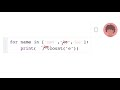
\includegraphics[width=\linewidth]{generated/youtube/youtube-list-vars-one.jpg}
\end{sbspanel}%
\begin{sbspanel}{0.21}%
\noindent
\includegraphics[width=\linewidth]{generated/qrcode/youtube-list-vars-one.png}
\href{https://pretextbook.org/examples/noparts/decorative/html/youtube-list-vars-one.html}{Standalone}%
\end{sbspanel}%
\end{sidebyside}%
\par
Width set at 40\%, so equal margins and thus centered.  Aenean faucibus augue tellus, et sollicitudin tortor finibus non. Maecenas semper dolor quis diam placerat, iaculis sollicitudin augue finibus. Vestibulum facilisis ligula lectus, ac tristique nisl aliquet non.%
\begin{sidebyside}{2}{0.075}{0.075}{0.17}%
\begin{sbspanel}{0.47}%
\noindent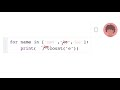
\includegraphics[width=\linewidth]{generated/youtube/youtube-list-vars-two.jpg}
\end{sbspanel}%
\begin{sbspanel}{0.21}%
\noindent
\includegraphics[width=\linewidth]{generated/qrcode/youtube-list-vars-two.png}
\href{https://pretextbook.org/examples/noparts/decorative/html/youtube-list-vars-two.html}{Standalone}%
\end{sbspanel}%
\end{sidebyside}%
\par
Asymmetric margins of 20\% and 40\% given, implying 40\% width, equal to previous instance.  Vivamus suscipit diam eget mi cursus viverra.%
\begin{sidebyside}{2}{0.075}{0.075}{0.17}%
\begin{sbspanel}{0.47}%
\noindent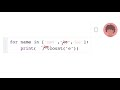
\includegraphics[width=\linewidth]{generated/youtube/youtube-list-vars-three.jpg}
\end{sbspanel}%
\begin{sbspanel}{0.21}%
\noindent
\includegraphics[width=\linewidth]{generated/qrcode/youtube-list-vars-three.png}
\href{https://pretextbook.org/examples/noparts/decorative/html/youtube-list-vars-three.html}{Standalone}%
\end{sbspanel}%
\end{sidebyside}%
\par
As a plain component of a \mono{<sidebyside>}.  Widths here are 20\% and 30\%, margins and gaps are automatic, default alignment on top edges.  Nulla pharetra imperdiet elit, in sodales nibh blandit ultricies. Maecenas efficitur ac felis ut pharetra.%
\begin{sidebyside}{2}{0.125}{0.125}{0.25}%
\end{sidebyside}%
\par
Inside a \mono{<figure>} with no adjustments, so default behavior.  Note how a \mono{<figure>} occupies the entire width of the page, so then does the caption.%
\begin{figureptx}{Figure}{List Variables}{atomic-video-13}{}%
\begin{sidebyside}{2}{0.075}{0.075}{0.17}%
\begin{sbspanel}{0.47}%
\noindent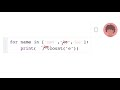
\includegraphics[width=\linewidth]{generated/youtube/youtube-list-vars-six.jpg}
\end{sbspanel}%
\begin{sbspanel}{0.21}%
\noindent
\includegraphics[width=\linewidth]{generated/qrcode/youtube-list-vars-six.png}
\href{https://pretextbook.org/examples/noparts/decorative/html/youtube-list-vars-six.html}{Standalone}%
\end{sbspanel}%
\end{sidebyside}%
\tcblower
\end{figureptx}%
Inside a \mono{<figure>} with asymmetric (large) margins of 30\% and 60\%.  Quisque finibus augue sit amet facilisis fringilla. Aenean faucibus augue tellus, et sollicitudin tortor finibus non.%
\begin{figureptx}{Figure}{List Variables}{atomic-video-15}{}%
\begin{sidebyside}{2}{0.075}{0.075}{0.17}%
\begin{sbspanel}{0.47}%
\noindent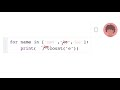
\includegraphics[width=\linewidth]{generated/youtube/youtube-list-vars-seven.jpg}
\end{sbspanel}%
\begin{sbspanel}{0.21}%
\noindent
\includegraphics[width=\linewidth]{generated/qrcode/youtube-list-vars-seven.png}
\href{https://pretextbook.org/examples/noparts/decorative/html/youtube-list-vars-seven.html}{Standalone}%
\end{sbspanel}%
\end{sidebyside}%
\tcblower
\end{figureptx}%
Inside figures inside a \mono{<sidebyside>}.  Same widths as previous \mono{<sidebyside>} but alignment on bottoms of the panels, to partially align captions.  Note how the captions are constrained in width by the width of the panels of the side-by-side.%
\begin{sidebyside}{2}{0.125}{0.125}{0.25}%
\begin{sbspanel}{0.2}[bottom]%
\begin{panelfigureptx}{Figure}{List Variables}{atomic-video-17-1}{}%
\begin{sidebyside}{2}{0.075}{0.075}{0.17}%
\begin{sbspanel}{0.47}%
\noindent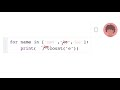
\includegraphics[width=\linewidth]{generated/youtube/youtube-list-vars-eight.jpg}
\end{sbspanel}%
\begin{sbspanel}{0.21}%
\noindent
\includegraphics[width=\linewidth]{generated/qrcode/youtube-list-vars-eight.png}
\href{https://pretextbook.org/examples/noparts/decorative/html/youtube-list-vars-eight.html}{Standalone}%
\end{sbspanel}%
\end{sidebyside}%
\tcblower
\end{panelfigureptx}%
\end{sbspanel}%
\begin{sbspanel}{0.3}[bottom]%
\begin{panelfigureptx}{Figure}{List Variables (Again)}{atomic-video-17-2}{}%
\begin{sidebyside}{2}{0.075}{0.075}{0.17}%
\begin{sbspanel}{0.47}%
\noindent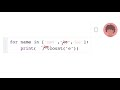
\includegraphics[width=\linewidth]{generated/youtube/youtube-list-vars-nine.jpg}
\end{sbspanel}%
\begin{sbspanel}{0.21}%
\noindent
\includegraphics[width=\linewidth]{generated/qrcode/youtube-list-vars-nine.png}
\href{https://pretextbook.org/examples/noparts/decorative/html/youtube-list-vars-nine.html}{Standalone}%
\end{sbspanel}%
\end{sidebyside}%
\tcblower
\end{panelfigureptx}%
\end{sbspanel}%
\end{sidebyside}%
\par
Identical code to previous example, but now wrapped in an overall \mono{<figure>}, which has its own caption and number, leaving the interior figures to be sub-numbered.  Cross-references use the full number: \hyperref[ups-video]{Figure~{\xreffont\ref{ups-video}}}.%
\begin{figureptx}{Figure}{Amalgamation of Videos}{atomic-video-19}{}%
\begin{sidebyside}{2}{0.125}{0.125}{0.25}%
\begin{sbspanel}{0.2}[bottom]%
\begin{subfigureptx}{Figure}{List Variables}{atomic-video-19-2-1}{}%
\begin{sidebyside}{2}{0.075}{0.075}{0.17}%
\begin{sbspanel}{0.47}%
\noindent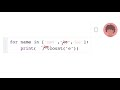
\includegraphics[width=\linewidth]{generated/youtube/youtube-list-vars-ten.jpg}
\end{sbspanel}%
\begin{sbspanel}{0.21}%
\noindent
\includegraphics[width=\linewidth]{generated/qrcode/youtube-list-vars-ten.png}
\href{https://pretextbook.org/examples/noparts/decorative/html/youtube-list-vars-ten.html}{Standalone}%
\end{sbspanel}%
\end{sidebyside}%
\tcblower
\end{subfigureptx}%
\end{sbspanel}%
\begin{sbspanel}{0.3}[bottom]%
\begin{subfigureptx}{Figure}{List Variables}{ups-video}{}%
\begin{sidebyside}{2}{0.075}{0.075}{0.17}%
\begin{sbspanel}{0.47}%
\noindent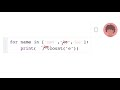
\includegraphics[width=\linewidth]{generated/youtube/youtube-list-vars-eleven.jpg}
\end{sbspanel}%
\begin{sbspanel}{0.21}%
\noindent
\includegraphics[width=\linewidth]{generated/qrcode/youtube-list-vars-eleven.png}
\href{https://pretextbook.org/examples/noparts/decorative/html/youtube-list-vars-eleven.html}{Standalone}%
\end{sbspanel}%
\end{sidebyside}%
\tcblower
\end{subfigureptx}%
\end{sbspanel}%
\end{sidebyside}%
\tcblower
\end{figureptx}%
\end{sectionptx}
%
%
\typeout{************************************************}
\typeout{Section 5.26 Runestone Assignment Testing}
\typeout{************************************************}
%
\begin{sectionptx}{Section}{Runestone Assignment Testing}{}{Runestone Assignment Testing}{}{}{section-runestone-assignment-testing}
This is a section that is specifically for testing when exercises are migrated to a Runestone Assignment page.%
%
%
\typeout{************************************************}
\typeout{Exercises 5.26 Exercises}
\typeout{************************************************}
%
\begin{exercises-subsection-numberless}{Exercises}{Exercises}{}{Exercises}{}{}{section-runestone-assignment-testing-3}
\begin{divisionexercise}{1}{}{}{exercisegroup-exercise-zero}%
This is an \mono{<exercises>} division (at the level of a \mono{<subsection>}) which is not being numbered.  We've hijacked this first exercise to say so, and to precede the \mono{<exercisegroup>} following, which is the real test right now. What is \(0+0\)?%
\end{divisionexercise}%
\par\medskip\noindent%
\textbf{An Exercise Group.}\space\space%
This introduction should appear ahead of each exercise when it shows up in the Runestone Assignment page.%
\begin{center}%
{\tabularfont%
\begin{tabular}{ll}
\((0,0)\)&\((0,1)\)\tabularnewline[0pt]
\((1,0)\)&\((1,1)\)
\end{tabular}
}%
\end{center}%
\begin{image}{0}{1}{0}{}%
\resizebox{\linewidth}{!}{%
\begin{tikzpicture}
    \draw[fill=blue!20] (0,0) -| (1,1) -| cycle;
\end{tikzpicture}%
}%
\end{image}%
It has a table, and an image too, to check it all comes through.%
\begin{exercisegroup}
\begin{divisionexerciseeg}{2}{}{}{exercisegroup-exercise-one}%
What is \(1+1\)?%
\par
%
\begin{enumerate}[label={\Alph*.}]
\item{}Two%
\item{}Three%
\end{enumerate}
%
\par\smallskip%
\noindent\textbf{\blocktitlefont Answer}.\hypertarget{exercisegroup-exercise-one-2}{}\quad{}A.%
\par\smallskip%
\noindent\textbf{\blocktitlefont Solution}.\hypertarget{exercisegroup-exercise-one-3}{}\quad{}%
\begin{enumerate}[label={\Alph*.}]
\item{}\lititle{Correct.}\par%
%
\item{}\lititle{Incorrect.}\par%
%
\end{enumerate}
%
\end{divisionexerciseeg}%
\begin{divisionexerciseeg}{3}{}{}{exercisegroup-exercise-two}%
What is \(2+2\)?%
\par
%
\begin{enumerate}[label={\Alph*.}]
\item{}Two%
\item{}Four%
\end{enumerate}
%
\par\smallskip%
\noindent\textbf{\blocktitlefont Answer}.\hypertarget{exercisegroup-exercise-two-2}{}\quad{}B.%
\par\smallskip%
\noindent\textbf{\blocktitlefont Solution}.\hypertarget{exercisegroup-exercise-two-3}{}\quad{}%
\begin{enumerate}[label={\Alph*.}]
\item{}\lititle{Incorrect.}\par%
%
\item{}\lititle{Correct.}\par%
%
\end{enumerate}
%
\end{divisionexerciseeg}%
\end{exercisegroup}
\par\medskip\noindent
\begin{divisionexercise}{4}{}{}{exercisegroup-exercise-three}%
What is \(3+3\)?%
\end{divisionexercise}%
\end{exercises-subsection-numberless}
And a final paragraph in the section, and a chance to say there is a trailing \mono{<exercise>} outside the \mono{<exercisegroup>}.%
\end{sectionptx}
%
%
\typeout{************************************************}
\typeout{Worksheet 5.27 A ``Group Work'' Worksheet}
\typeout{************************************************}
%
\newgeometry{left=0.75in, right=0.75in, top=0.75in, bottom=0.75in}
\begin{worksheet-section}{Worksheet}{A ``Group Work'' Worksheet}{}{A ``Group Work'' Worksheet}{}{}{worksheet-groupwork}
This is a \mono{<worksheet>} which has a \mono{@groupwork} attribute set to \mono{yes}, along with a \mono{@label} attribute to assist with the Runestone database.  Note, you can also set a \mono{@groupsize} attribute.  When hosted on Runestone, the exercises within will be available for a group of students to submit together.%
\begin{divisionexercise}{1}{Multiple-Choice, Group Work.}{}{groupwork-multiple-choice}%
\index{stop signs}%
\index{group work}%
What color is a stop sign?%
\par
%
\begin{enumerate}[label={\Alph*.}]
\item{}Green%
\item{}Red%
\item{}White%
\end{enumerate}
%
\par\smallskip%
\noindent\textbf{\blocktitlefont Hint 1}.\hypertarget{groupwork-multiple-choice-5}{}\quad{}What did you see last time you went driving?%
\par\smallskip%
\noindent\textbf{\blocktitlefont Hint 2}.\hypertarget{groupwork-multiple-choice-6}{}\quad{}Maybe go out for a drive?%
\par\smallskip%
\noindent\textbf{\blocktitlefont Answer}.\hypertarget{groupwork-multiple-choice-7}{}\quad{}B.%
\par\smallskip%
\noindent\textbf{\blocktitlefont Solution}.\hypertarget{groupwork-multiple-choice-8}{}\quad{}%
\begin{enumerate}[label={\Alph*.}]
\item{}\lititle{Incorrect.}\par%
Green means ``go!''.%
\item{}\lititle{Correct.}\par%
Red is universally used for prohibited activities or serious warnings.%
\item{}\lititle{Incorrect.}\par%
White might be hard to see.%
\end{enumerate}
%
\end{divisionexercise}%
Worksheets allow for material interleaved with the \mono{<exercise>} throughout.%
\begin{divisionexercise}{2}{Parsons Problem, Group Work.}{}{groupwork-number-theory}%
\index{even numbers}%
\index{groupwork}%
Create a proof of the theorem: If \(n\) is an even number, then \(n\equiv 0\mod 2\).%
\par
%
\begin{itemize}[label=\textbullet]
\item{}Click the heels of your ruby slippers together three times.%
\item{}Suppose \(n\) is even.%
\item{}%
\begin{itemize}[label=]
\item{}Either:%
\par
Then \(n\) is a prime number.%
\item{}Or:%
\par
Then there exists an \(m\) so that \(n = 2m\).%
\item{}Or:%
\par
Then there exists an \(m\) so that \(n = 2m + 1\).%
\end{itemize}
%
\item{}Thus \(n\equiv 0\mod 2\).%
\item{}So \(n = 2m + 0\).%
\par
This is a superfluous second paragraph in this block.%
\item{}And a little bit of irrelevant multi-line math%
\begin{align*}
c^2&a^2+b^2\\
&x^2+y^2\text{.}
\end{align*}
%
\end{itemize}
%
\par\smallskip%
\noindent\textbf{\blocktitlefont Solution}.\hypertarget{groupwork-number-theory-5}{}\quad{}%
\begin{itemize}[label=\textbullet]
\item{}Suppose \(n\) is even.%
\item{}Then there exists an \(m\) so that \(n = 2m\).%
\item{}So \(n = 2m + 0\).%
\par
This is a superfluous second paragraph in this block.%
\item{}Thus \(n\equiv 0\mod 2\).%
\end{itemize}
%
\end{divisionexercise}%
\end{worksheet-section}
\restoregeometry
%
%
\typeout{************************************************}
\typeout{Exercises 5.28 Group Exercises}
\typeout{************************************************}
%
\begin{exercises-section}{Exercises}{Group Exercises}{}{Group Exercises}{}{}{exercises-title-groupwork}
\begin{introduction}{}%
This is an \mono{<exercises>} division with no \mono{<title>}, set as groupwork, and therefore its default title will automatically indicate it is meant for a group.  Otherwise, it is not of any new interest.%
\end{introduction}%
\begin{divisionexercise}{1}{Multiple-Choice, Not Randomized, One Answer.}{}{multiple-choice-not-randomized-five}%
\index{stop signs}%
What color is a stop sign?%
\par
%
\begin{enumerate}[label={\Alph*.}]
\item{}Green%
\item{}Red%
\item{}White%
\end{enumerate}
%
\par\smallskip%
\noindent\textbf{\blocktitlefont Hint 1}.\hypertarget{multiple-choice-not-randomized-five-4}{}\quad{}What did you see last time you went driving?%
\par\smallskip%
\noindent\textbf{\blocktitlefont Hint 2}.\hypertarget{multiple-choice-not-randomized-five-5}{}\quad{}Maybe go out for a drive?%
\par\smallskip%
\noindent\textbf{\blocktitlefont Answer}.\hypertarget{multiple-choice-not-randomized-five-6}{}\quad{}B.%
\par\smallskip%
\noindent\textbf{\blocktitlefont Solution}.\hypertarget{multiple-choice-not-randomized-five-7}{}\quad{}%
\begin{enumerate}[label={\Alph*.}]
\item{}\lititle{Incorrect.}\par%
Green means ``go!''.%
\item{}\lititle{Correct.}\par%
Red is universally used for prohibited activities or serious warnings.%
\item{}\lititle{Incorrect.}\par%
White might be hard to see.%
\end{enumerate}
%
\end{divisionexercise}%
\end{exercises-section}
%
%
\typeout{************************************************}
\typeout{Section 5.29 SPLICE Integration}
\typeout{************************************************}
%
\begin{sectionptx}{Section}{SPLICE Integration}{}{SPLICE Integration}{}{}{splice-integration}
\href{https://cssplice.org/}{SPLICE}\footnote{\nolinkurl{cssplice.org}\label{splice-integration-2-2}} is a project to supply documentation and infrastructure to help with adopting shared standards, protocols, and tools for web-based learning tools. The project has designed a \href{https://cssplice.org/slcp/index.html}{protocol}\footnote{\nolinkurl{cssplice.org/slcp}\label{splice-integration-2-4}} for an embedded iframe to communicate with its host page.%
\par
One aspect is the ability of an iframe to ask for a new size. Below is a test of that capability.%
\par
These are examples that use the \href{https://cssplice.org/slcp/index.html}{SPLICE}\footnote{\nolinkurl{cssplice.org/slcp}\label{splice-integration-4-2}} protocol for communicating with a server, such as Runestone. They are all integrated into this PreTeXt book as an \mono{<interactive>} that uses an \mono{@iframe} attribute to embed an iframe from some other server.%
\par
This first sample tests the ability of an iframe to ask for a new size.%
\begin{sidebyside}{2}{0.075}{0.075}{0.17}%
\begin{sbspanel}{0.47}%
\noindent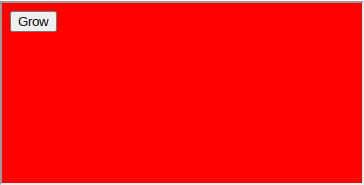
\includegraphics[width=\linewidth]{generated/preview/splice-resize-example-preview.png}
\end{sbspanel}%
\begin{sbspanel}{0.21}%
\noindent
\includegraphics[width=\linewidth]{generated/qrcode/splice-resize-example.png}
\href{https://pretextbook.org/examples/noparts/decorative/html/splice-resize-example.html}{Standalone}%
\par
\href{https://pretextbook.org/examples/noparts/decorative/html/splice-resize-example-if.html}{Embed}%
\end{sbspanel}%
\end{sidebyside}%
\par
The next uses \href{https://codecheck.io}{CodeCheck}\footnote{\nolinkurl{codecheck.io}\label{splice-integration-7-2}}.%
\begin{figureptx}{Figure}{CodeCheck \mono{iframe}}{horstmann-codecheck}{}%
\begin{sidebyside}{2}{0.075}{0.075}{0.17}%
\begin{sbspanel}{0.47}%
\noindent
\includegraphics[width=\linewidth]{generated/preview/interactive-horstmann-codecheck-preview.png}
\end{sbspanel}%
\begin{sbspanel}{0.21}%
\noindent
\includegraphics[width=\linewidth]{generated/qrcode/interactive-horstmann-codecheck.png}
\href{https://pretextbook.org/examples/noparts/decorative/html/interactive-horstmann-codecheck.html}{Standalone}%
\end{sbspanel}%
\end{sidebyside}%
\tcblower
\end{figureptx}%
And the remaing four are from the \href{https://opendsax.cs.vt.edu/}{OpenDSA}\footnote{\nolinkurl{opendsax.cs.vt.edu}\label{splice-integration-9-2}} project.%
\begin{figureptx}{Figure}{Stack pop slideshow}{opendsa-slideshow}{}%
\begin{sidebyside}{2}{0.075}{0.075}{0.17}%
\begin{sbspanel}{0.47}%
\noindent
\includegraphics[width=\linewidth]{generated/preview/opendsa-slideshow-pop-preview.png}
\end{sbspanel}%
\begin{sbspanel}{0.21}%
\noindent
\includegraphics[width=\linewidth]{generated/qrcode/opendsa-slideshow-pop.png}
\href{https://pretextbook.org/examples/noparts/decorative/html/opendsa-slideshow-pop.html}{Standalone}%
\end{sbspanel}%
\end{sidebyside}%
\tcblower
\end{figureptx}%
\begin{figureptx}{Figure}{A List Insertion Exercise}{splice-integration-insert}{}%
\begin{sidebyside}{2}{0.075}{0.075}{0.17}%
\begin{sbspanel}{0.47}%
\noindent
\includegraphics[width=\linewidth]{generated/preview/OpenDSA-list-insertion-preview.png}
\end{sbspanel}%
\begin{sbspanel}{0.21}%
\noindent
\includegraphics[width=\linewidth]{generated/qrcode/OpenDSA-list-insertion.png}
\href{https://pretextbook.org/examples/noparts/decorative/html/OpenDSA-list-insertion.html}{Standalone}%
\end{sbspanel}%
\end{sidebyside}%
\tcblower
\end{figureptx}%
\begin{figureptx}{Figure}{A Binary Search Exercise}{splice-integration-bs}{}%
\begin{sidebyside}{2}{0.075}{0.075}{0.17}%
\begin{sbspanel}{0.47}%
\noindent
\includegraphics[width=\linewidth]{generated/preview/OpenDSA-integration-bs-preview.png}
\end{sbspanel}%
\begin{sbspanel}{0.21}%
\noindent
\includegraphics[width=\linewidth]{generated/qrcode/OpenDSA-integration-bs.png}
\href{https://pretextbook.org/examples/noparts/decorative/html/OpenDSA-integration-bs.html}{Standalone}%
\end{sbspanel}%
\end{sidebyside}%
\tcblower
\end{figureptx}%
\begin{figureptx}{Figure}{Dijkstra's Algorithm Exercise}{splice-integration-dijkstra}{}%
\begin{sidebyside}{2}{0.075}{0.075}{0.17}%
\begin{sbspanel}{0.47}%
\noindent
\includegraphics[width=\linewidth]{generated/preview/OpenDSA-integration-dijkstra-preview.png}
\end{sbspanel}%
\begin{sbspanel}{0.21}%
\noindent
\includegraphics[width=\linewidth]{generated/qrcode/OpenDSA-integration-dijkstra.png}
\href{https://pretextbook.org/examples/noparts/decorative/html/OpenDSA-integration-dijkstra.html}{Standalone}%
\end{sbspanel}%
\end{sidebyside}%
\tcblower
\end{figureptx}%
\end{sectionptx}
%
%
\typeout{************************************************}
\typeout{Exercises 5.30 Timed Chapter Exam}
\typeout{************************************************}
%
\begin{exercises-section}{Exercises}{Timed Chapter Exam}{}{Timed Chapter Exam}{}{}{chapter-exam}
\begin{introduction}{}%
This is an \mono{<exercises>} division, as a peer of the \mono{<section>} in this \mono{<chapter>} of a \mono{<book>}.  It is also setup as a Runestone timed exam.  So it is an example of how you might have a per-chapter exam.  This contrasts with an earlier timed exam which is constructed as a per-section exam (\hyperlink{timed-exercises}{Exercises~{\xreffont 5.21}}).  The exercises are the same here, but in a different order.  As a test, this exam is ``pauseable'' and has a 15 minute time limit.%
\end{introduction}%
\begin{divisionexercise}{1}{Multiple-Choice, Not Randomized, One Answer.}{}{multiple-choice-not-randomized-timed-two}%
\index{stop signs}%
What color is a stop sign?%
\par
%
\begin{enumerate}[label={\Alph*.}]
\item{}Green%
\item{}Red%
\item{}White%
\end{enumerate}
%
\par\smallskip%
\noindent\textbf{\blocktitlefont Hint 1}.\hypertarget{multiple-choice-not-randomized-timed-two-4}{}\quad{}What did you see last time you went driving?%
\par\smallskip%
\noindent\textbf{\blocktitlefont Hint 2}.\hypertarget{multiple-choice-not-randomized-timed-two-5}{}\quad{}Maybe go out for a drive?%
\par\smallskip%
\noindent\textbf{\blocktitlefont Answer}.\hypertarget{multiple-choice-not-randomized-timed-two-6}{}\quad{}B.%
\par\smallskip%
\noindent\textbf{\blocktitlefont Solution}.\hypertarget{multiple-choice-not-randomized-timed-two-7}{}\quad{}%
\begin{enumerate}[label={\Alph*.}]
\item{}\lititle{Incorrect.}\par%
Green means ``go!''.%
\item{}\lititle{Correct.}\par%
Red is universally used for prohibited activities or serious warnings.%
\item{}\lititle{Incorrect.}\par%
White might be hard to see.%
\end{enumerate}
%
\end{divisionexercise}%
\begin{divisionexercise}{2}{True\slash{}False.}{}{vector-space-dimension-timed-two}%
\index{vector space}%
True or False?%
\par
Every vector space has finite dimension.%
\par\smallskip%
\noindent\textbf{\blocktitlefont Hint}.\hypertarget{vector-space-dimension-timed-two-4}{}\quad{}\(P_n\), the vector space of polynomials with degree at most \(n\), has dimension \(n+1\) by \hyperref[theorem-exponent-laws]{Theorem~{\xreffont\ref{theorem-exponent-laws}}}.  [Cross-reference is just a demo, content is not relevant.]  What happens if we relax the defintion and remove the parameter \(n\)?%
\par\smallskip%
\noindent\textbf{\blocktitlefont Answer}.\hypertarget{vector-space-dimension-timed-two-5}{}\quad{}False.%
\par\smallskip%
\noindent\textbf{\blocktitlefont Solution}.\hypertarget{vector-space-dimension-timed-two-6}{}\quad{}False.%
\par
The vector space of all polynomials with finite degree has a basis, \(B = \{1,x,x^2,x^3,\dots\}\), which is infinte.%
\end{divisionexercise}%
\end{exercises-section}
\end{chapterptx}
%
\appendix%
%
\clearpage\phantomsection%
\addcontentsline{toc}{part}{Appendices}%
%
%
\typeout{************************************************}
\typeout{Appendix A Notation}
\typeout{************************************************}
%
\begin{appendixptx}{Appendix}{Notation}{}{Notation}{}{}{backmatter-2}
\renewcommand*{\appendixname}{Appendix}
The following table defines the notation used in this book. Page numbers or references refer to the first appearance of each symbol.%
\begin{longtable}[l]{lp{0.60\textwidth}r}
\addtocounter{table}{-1}
\textbf{Symbol}&\textbf{Description}&\textbf{Page}\\[1em]
\endfirsthead
\textbf{Symbol}&\textbf{Description}&\textbf{Page}\\[1em]
\endhead
\multicolumn{3}{r}{(Continued on next page)}\\
\endfoot
\endlastfoot
\(a \in A\)&\(a\) is in the set \(A\)&\pageref{section-sets-and-equivalence-relations-2-2-11}\\
\({\mathbb N}\)&the natural numbers&\pageref{section-sets-and-equivalence-relations-2-4-2}\\
\({\mathbb Z}\)&the integers&\pageref{section-sets-and-equivalence-relations-2-4-3}\\
\({\mathbb Q}\)&the rational numbers&\pageref{section-sets-and-equivalence-relations-2-4-4}\\
\({\mathbb R}\)&the real numbers&\pageref{section-sets-and-equivalence-relations-2-4-5}\\
\({\mathbb C}\)&the complex numbers&\pageref{section-sets-and-equivalence-relations-2-4-6}\\
\(A \subset B\)&\(A\) is a subset of \(B\)&\pageref{section-sets-and-equivalence-relations-2-5-8}\\
\(\emptyset\)&the empty set&\pageref{section-sets-and-equivalence-relations-2-6-3}\\
\(A \cup B\)&the union of sets \(A\) and \(B\)&\pageref{section-sets-and-equivalence-relations-2-7-10}\\
\(A \cap B\)&the intersection of sets \(A\) and \(B\)&\pageref{section-sets-and-equivalence-relations-2-7-11}\\
\(A'\)&complement of the set \(A\)&\pageref{section-sets-and-equivalence-relations-2-9-7}\\
\(A \setminus B\)&difference between sets \(A\) and \(B\)&\pageref{section-sets-and-equivalence-relations-2-10-4}\\
\(A \times B\)&Cartesian product of sets \(A\) and \(B\)&\pageref{section-sets-and-equivalence-relations-3-2-7}\\
\(A^n\)&\(A \times \cdots \times A\) (\(n\) times)&\pageref{section-sets-and-equivalence-relations-3-4-8}\\
\(id\)&identity mapping&\pageref{section-sets-and-equivalence-relations-3-20-19}\\
\(f^{-1}\)&inverse of the function \(f\)&\pageref{section-sets-and-equivalence-relations-3-20-20}\\
\(a \equiv b \pmod{n}\)&\(a\) is congruent to \(b\) modulo \(n\)&\pageref{example-sets-congruent-integers-2-18}\\
\(n!\)&\(n\) factorial&\pageref{example-integers-binomial-theorem-2-8}\\
\(\binom{n}{k}\)&binomial coefficient \(n!/(k!(n-k)!)\)&\pageref{example-integers-binomial-theorem-2-9}\\
\(a \mid b\)&\(a\) divides \(b\)&\pageref{section-division-algorithm-2-3-24}\\
\(\gcd(a, b)\)&greatest common divisor of \(a\) and \(b\)&\pageref{section-division-algorithm-2-3-25}\\
\(\mathcal P(X)\)&power set of \(X\)&\pageref{exercises-integers-13-2-1-6}\\
\(\lcm(m,n)\)&the least common multiple of \(m\) and \(n\)&\pageref{exercises-integers-24-1-1-14}\\
\(\mathbb Z_n\)&the integers modulo \(n\)&\pageref{section-mod-n-sym-5-4-10}\\
\(U(n)\)&group of units in \(\mathbb Z_n\)&\pageref{example-groups-z6-mult-3-8}\\
\(\mathbb M_n(\mathbb R)\)&the \(n \times n\) matrices with entries in \(\mathbb R\)&\pageref{example-groups-gl2-2-5}\\
\(\det A\)&the determinant of \(A\)&\pageref{example-groups-gl2-2-15}\\
\(GL_n(\mathbb R)\)&the general linear group&\pageref{example-groups-gl2-2-18}\\
\(Q_8\)&the group of quaternions&\pageref{example-groups-quaterions-2-13}\\
\(\mathbb C^*\)&the multiplicative group of complex numbers&\pageref{example-groups-c-star-2-2}\\
\(|G|\)&the order of a group&\pageref{section-groups-define-3-11-12}\\
\(\mathbb R^*\)&the multiplicative group of real numbers&\pageref{example-groups-multiplicative-subgroup-2-2}\\
\(\mathbb Q^*\)&the multiplicative group of rational numbers&\pageref{example-groups-multiplicative-subgroup-2-7}\\
\(SL_n(\mathbb R)\)&the special linear group&\pageref{example-groups-sl2-2-3}\\
\(Z(G)\)&the center of a group&\pageref{exercises-groups-49-1-1-7}\\
\(\langle a \rangle\)&cyclic group generated by \(a\)&\pageref{theorem-cyclic-subgroup-1-1-9}\\
\(|a|\)&the order of an element \(a\)&\pageref{cyclic-4-7-24}\\
\(\cis \theta\)&\(\cos \theta + i \sin \theta\)&\pageref{cyclic-6-9-14}\\
\(\mathbb T\)&the circle group&\pageref{cyclic-6-16-9}\\
\end{longtable}
\end{appendixptx}
%
%
\typeout{************************************************}
\typeout{Appendix B Hints and Answers to Selected Odd Exercises}
\typeout{************************************************}
%
\begin{solutions-chapter}{Appendix}{Hints and Answers to Selected Odd Exercises}{}{Hints and Answers to Selected Odd Exercises}{}{}{backmatter-3}
\par\medskip
\noindent\textbf{\Large{}2\space\textperiodcentered\space{}The Integers\\
2.4\space\textperiodcentered\space{}Exercises}
\begin{divisionsolution}{Exercise}{2.4.1}{}{exercises-integers-2}%
\noindent\textbf{\blocktitlefont Answer}.\hypertarget{exercises-integers-2-2-back}{}\quad{}The base case, \(S(1): [1(1 + 1)(2(1) + 1)]/6 = 1 = 1^2\) is true.%
\par
Assume that \(S(k): 1^2 + 2^2 + \cdots + k^2 = [k(k + 1)(2k + 1)]/6\) is true. Then%
\begin{align*}
1^2 + 2^2 + \cdots + k^2 + (k + 1)^2 & = [k(k + 1)(2k + 1)]/6 + (k + 1)^2\\
& = [(k + 1)((k + 1) + 1)(2(k + 1) + 1)]/6,
\end{align*}
and so \(S(k + 1)\) is true. Thus, \(S(n)\) is true for all positive integers \(n\).%
\end{divisionsolution}%
\begin{divisionsolution}{Exercise}{2.4.3}{}{exercises-integers-4}%
\noindent\textbf{\blocktitlefont Answer}.\hypertarget{exercises-integers-4-2-back}{}\quad{}The base case, \(S(4): 4! = 24 \gt 16 =2^4\) is true. Assume \(S(k): k! \gt 2^k\) is true. Then \((k + 1)! = k! (k + 1) \gt 2^k \cdot 2 = 2^{k + 1}\), so \(S(k + 1)\) is true. Thus, \(S(n)\) is true for all positive integers \(n\).%
\end{divisionsolution}%
\begin{divisionsolution}{Exercise}{2.4.9}{}{exercises-integers-10}%
\noindent\textbf{\blocktitlefont Hint}.\hypertarget{exercises-integers-10-2-back}{}\quad{}Follow the proof in \hyperref[example-integers-binomial-theorem]{Example~{\xreffont\ref{example-integers-binomial-theorem}}}.%
\end{divisionsolution}%
\begin{divisionsolution}{Exercise}{2.4.11}{}{exercises-integers-12}%
\noindent\textbf{\blocktitlefont Hint}.\hypertarget{exercises-integers-12-2-back}{}\quad{}The base case, \(S(0): (1 + x)^0 - 1 = 0 \geq 0 = 0 \cdot x\) is true. Assume \(S(k): (1 + x)^k -1 \geq kx\) is true. Then%
\begin{align*}
(1 + x)^{k + 1} - 1 & = (1 + x)(1 + x)^k -1\\
& = (1 + x)^k + x(1 + x)^k - 1\\
& \geq kx + x(1 + x)^k\\
& \geq kx + x\\
& = (k + 1)x,
\end{align*}
so \(S(k + 1)\) is true. Therefore, \(S(n)\) is true for all positive integers \(n\).%
\end{divisionsolution}%
\begin{divisionsolution}{Exercise}{2.4.17}{Fibonacci Numbers.}{exercises-integers-18}%
\par\smallskip%
\noindent\textbf{\blocktitlefont Hint}.\hypertarget{exercises-integers-18-3-back}{}\quad{}For \hyperlink{fn_ineq}{Item~{\xreffont 2.4.17.a}} and \hyperlink{fn_prod}{Item~{\xreffont 2.4.17.b}} use mathematical induction. \hyperlink{fn_formula}{Item~{\xreffont 2.4.17.c}} Show that \(f_1 = 1\), \(f_2 = 1\), and \(f_{n + 2} = f_{n + 1} + f_n\). \hyperlink{fn_ratio}{Item~{\xreffont 2.4.17.d}}  Use part \hyperlink{fn_formula}{Item~{\xreffont 2.4.17.c}}. \hyperlink{fn_coprime}{Item~{\xreffont 2.4.17.e}} Use part \hyperlink{fn_prod}{Item~{\xreffont 2.4.17.b}} and \hyperlink{exercise-integers-gcd-1}{Exercise~{\xreffont 2.4.16}}.%
\end{divisionsolution}%
\begin{divisionsolution}{Exercise}{2.4.19}{}{exercises-integers-20}%
\noindent\textbf{\blocktitlefont Hint}.\hypertarget{exercises-integers-20-2-back}{}\quad{}Use the Fundamental Theorem of Arithmetic.%
\end{divisionsolution}%
\begin{divisionsolution}{Exercise}{2.4.23}{}{exercises-integers-24}%
\noindent\textbf{\blocktitlefont Hint}.\hypertarget{exercises-integers-24-2-back}{}\quad{}Let \(S = \{s \in {\mathbb N} : a \mid s\), \(b \mid s \}\). Then \(S \neq \emptyset\), since \(|ab| \in S\). By the Principle of Well-Ordering, \(S\) contains a least element \(m\). To show uniqueness, suppose that \(a \mid n\) and \(b \mid n\) for some \(n \in {\mathbb N}\). By the division algorithm, there exist unique integers \(q\) and \(r\) such that \(n = mq + r\), where \(0 \leq r \lt m\). Since \(a\) and \(b\) divide both \(m\), and \(n\), it must be the case that  \(a\) and \(b\) both divide \(r\).  Thus, \(r = 0\) by the minimality of \(m\). Therefore, \(m \mid n\).%
\end{divisionsolution}%
\begin{divisionsolution}{Exercise}{2.4.27}{}{exercises-integers-28}%
\noindent\textbf{\blocktitlefont Hint}.\hypertarget{exercises-integers-28-2-back}{}\quad{}Since \(\gcd(a,b) = 1\), there exist integers \(r\) and \(s\) such that \(ar + bs = 1\).   Thus, \(acr + bcs = c\). Since \(a\) divides both \(bc\) and itself, \(a\) must divide \(c\).%
\end{divisionsolution}%
\begin{divisionsolution}{Exercise}{2.4.29}{}{exercises-integers-30}%
\noindent\textbf{\blocktitlefont Hint}.\hypertarget{exercises-integers-30-2-back}{}\quad{}Every prime must be of the form 2, 3, \(6n + 1\), or \(6n + 5\).   Suppose there are only finitely many primes of the form \(6k + 5\).%
\end{divisionsolution}%
\par\medskip
\noindent\textbf{\Large{}3\space\textperiodcentered\space{}Groups\\
3.5\space\textperiodcentered\space{}Exercises}
\begin{divisionsolution}{Exercise}{3.5.1}{}{exercises-groups-2}%
\noindent\textbf{\blocktitlefont Hint}.\hypertarget{exercises-groups-2-2-back}{}\quad{}(a) \(3 + 7 \mathbb Z = \{ \ldots, -4, 3, 10, \ldots \}\);  (c) \(18 + 26 \mathbb Z\);  (e) \(5 + 6 \mathbb Z\).%
\end{divisionsolution}%
\begin{divisionsolution}{Exercise}{3.5.15}{}{exercises-groups-16}%
\noindent\textbf{\blocktitlefont Hint}.\hypertarget{exercises-groups-16-2-back}{}\quad{}There is a nonabelian group containing six elements.%
\end{divisionsolution}%
\begin{divisionsolution}{Exercise}{3.5.17}{}{exercises-groups-18}%
\noindent\textbf{\blocktitlefont Hint}.\hypertarget{exercises-groups-18-2-back}{}\quad{}The are five different groups of order 8.%
\end{divisionsolution}%
\begin{divisionsolution}{Exercise}{3.5.25}{}{exercises-groups-26}%
\noindent\textbf{\blocktitlefont Hint}.\hypertarget{exercises-groups-26-2-back}{}\quad{}%
\begin{align*}
(aba^{-1})^n & = (aba^{-1})(aba^{-1}) \cdots (aba^{-1})\\
& = ab(aa^{-1})b(aa^{-1})b \cdots b(aa^{-1})ba^{-1}\\
& = ab^na^{-1}.
\end{align*}
%
\end{divisionsolution}%
\begin{divisionsolution}{Exercise}{3.5.31}{}{exercises-groups-32}%
\noindent\textbf{\blocktitlefont Hint}.\hypertarget{exercises-groups-32-2-back}{}\quad{}Since \(abab = (ab)^2 = e = a^2 b^2 = aabb\), we know that \(ba = ab\).%
\end{divisionsolution}%
\begin{divisionsolution}{Exercise}{3.5.35}{}{exercises-groups-36}%
\noindent\textbf{\blocktitlefont Hint}.\hypertarget{exercises-groups-36-2-back}{}\quad{}\(H_1 = \{ id \}\), \(H_2 = \{ id, \rho_1, \rho_2 \}\), \(H_3 = \{ id, \mu_1 \}\), \(H_4 = \{ id, \mu_2 \}\), \(H_5 = \{ id, \mu_3 \}\), \(S_3\).%
\end{divisionsolution}%
\begin{divisionsolution}{Exercise}{3.5.41}{}{exercises-groups-42}%
\noindent\textbf{\blocktitlefont Hint}.\hypertarget{exercises-groups-42-2-back}{}\quad{}The identity of \(G\) is \(1 = 1 + 0 \sqrt{2}\). Since \((a + b \sqrt{2}\, )(c + d \sqrt{2}\, ) = (ac + 2bd) + (ad + bc)\sqrt{2}\), \(G\) is closed under multiplication.  Finally,  \((a + b \sqrt{2}\, )^{-1} = a/(a^2 - 2b^2) - b\sqrt{2}/(a^2 - 2 b^2)\).%
\end{divisionsolution}%
\begin{divisionsolution}{Exercise}{3.5.49}{}{exercises-groups-50}%
\noindent\textbf{\blocktitlefont Hint}.\hypertarget{exercises-groups-50-2-back}{}\quad{}Since \(a^4b = ba\), it must be the case that \(b = a^6 b = a^2 b a\), and we can conclude that \(ab = a^3 b a = ba\).%
\end{divisionsolution}%
\begin{exercisegroupcol}{2}
\begin{divisionsolutionegcol}{Exercise}{3.5.55}{}{exercises-groups-56-2}%
\noindent\textbf{\blocktitlefont Answer}.\hypertarget{exercises-groups-56-2-2-back}{}\quad{}\(1\)%
\end{divisionsolutionegcol}%
\begin{divisionsolutionegcol}{Exercise}{3.5.57}{}{exercises-groups-56-4}%
\noindent\textbf{\blocktitlefont Answer}.\hypertarget{exercises-groups-56-4-2-back}{}\quad{}\(n\)%
\end{divisionsolutionegcol}%
\end{exercisegroupcol}
\par\medskip\noindent
\begin{divisionsolution}{Exercise}{3.5.59}{}{exercises-groups-57}%
\begin{enumerate}[font=\bfseries,label=(\alph*),ref=\alph*]%
\item[(a)]\noindent\textbf{\blocktitlefont Answer}.\hypertarget{exercises-groups-57-2-2-back}{}\quad{}\(2\)%
\item[(b)]\begin{enumerate}[font=\bfseries,label=(\roman*),ref=\theenumi.\roman*]%
\item[(i)]\noindent\textbf{\blocktitlefont Answer}.\hypertarget{exercises-groups-57-3-2-2-back}{}\quad{}\(6\)%
\item[(ii)]\noindent\textbf{\blocktitlefont Answer}.\hypertarget{exercises-groups-57-3-3-2-back}{}\quad{}\(10\)%
\end{enumerate}%
\end{enumerate}%
\end{divisionsolution}%
\par\medskip
\noindent\textbf{\Large{}5\space\textperiodcentered\space{}Runestone Testing\\
5.8\space\textperiodcentered\space{}True\slash{}False Exercises}
\begin{divisionsolution}{Exercise}{5.8.1}{True\slash{}False.}{vector-space-dimension}%
\par\smallskip%
\noindent\textbf{\blocktitlefont Hint}.\hypertarget{vector-space-dimension-4-back}{}\quad{}\(P_n\), the vector space of polynomials with degree at most \(n\), has dimension \(n+1\) by \hyperref[theorem-exponent-laws]{Theorem~{\xreffont\ref{theorem-exponent-laws}}}.  [Cross-reference is just a demo, content is not relevant.]  What happens if we relax the defintion and remove the parameter \(n\)?%
\par\smallskip%
\noindent\textbf{\blocktitlefont Answer}.\hypertarget{vector-space-dimension-5-back}{}\quad{}False.%
\par\smallskip%
\noindent\textbf{\blocktitlefont Solution}.\hypertarget{vector-space-dimension-6-back}{}\quad{}False.%
\par
The vector space of all polynomials with finite degree has a basis, \(B = \{1,x,x^2,x^3,\dots\}\), which is infinte.%
\end{divisionsolution}%
\par\medskip
\noindent\textbf{\Large{}5.9\space\textperiodcentered\space{}Multiple Choice Exercises}
\begin{divisionsolution}{Exercise}{5.9.1}{Multiple-Choice, Not Randomized, One Answer.}{multiple-choice-not-randomized}%
\par\smallskip%
\noindent\textbf{\blocktitlefont Hint 1}.\hypertarget{multiple-choice-not-randomized-4-back}{}\quad{}What did you see last time you went driving?%
\par\smallskip%
\noindent\textbf{\blocktitlefont Hint 2}.\hypertarget{multiple-choice-not-randomized-5-back}{}\quad{}Maybe go out for a drive?%
\par\smallskip%
\noindent\textbf{\blocktitlefont Answer}.\hypertarget{multiple-choice-not-randomized-6-back}{}\quad{}B.%
\par\smallskip%
\noindent\textbf{\blocktitlefont Solution}.\hypertarget{multiple-choice-not-randomized-7-back}{}\quad{}%
\begin{enumerate}[label={\Alph*.}]
\item{}\lititle{Incorrect.}\par%
Green means ``go!''.%
\item{}\lititle{Correct.}\par%
Red is universally used for prohibited activities or serious warnings.%
\item{}\lititle{Incorrect.}\par%
White might be hard to see.%
\end{enumerate}
%
\end{divisionsolution}%
\begin{divisionsolution}{Exercise}{5.9.3}{Multiple-Choice, Not Randomized, Multiple Answers.}{multiple-choice-multiple-answers}%
\par\smallskip%
\noindent\textbf{\blocktitlefont Hint}.\hypertarget{multiple-choice-multiple-answers-4-back}{}\quad{}Do you know the acronym\textellipsis{}\acronym{ROY G BIV} for the colors of a rainbow, and their order?%
\par\smallskip%
\noindent\textbf{\blocktitlefont Answer}.\hypertarget{multiple-choice-multiple-answers-5-back}{}\quad{}A, B, D.%
\par\smallskip%
\noindent\textbf{\blocktitlefont Solution}.\hypertarget{multiple-choice-multiple-answers-6-back}{}\quad{}%
\begin{enumerate}[label={\Alph*.}]
\item{}\lititle{Correct.}\par%
Red is a definitely one of the colors.%
\item{}\lititle{Correct.}\par%
Yes, yellow is correct.%
\item{}\lititle{Incorrect.}\par%
Remember the acronym\textellipsis{}\acronym{ROY G BIV}.  ``B'' stands for blue.%
\item{}\lititle{Correct.}\par%
Yes, green is one of the colors.%
\end{enumerate}
%
\end{divisionsolution}%
\begin{divisionsolution}{Exercise}{5.9.5}{Multiple-Choice, Randomized, One Answer but with Checkboxes.}{multiple-choice-randomized-forced-checkbox}%
\par\smallskip%
\noindent\textbf{\blocktitlefont Hint 1}.\hypertarget{multiple-choice-randomized-forced-checkbox-4-back}{}\quad{}What did you see last time you went driving?%
\par\smallskip%
\noindent\textbf{\blocktitlefont Hint 2}.\hypertarget{multiple-choice-randomized-forced-checkbox-5-back}{}\quad{}Maybe go out for a drive?%
\par\smallskip%
\noindent\textbf{\blocktitlefont Answer}.\hypertarget{multiple-choice-randomized-forced-checkbox-6-back}{}\quad{}B.%
\par\smallskip%
\noindent\textbf{\blocktitlefont Solution}.\hypertarget{multiple-choice-randomized-forced-checkbox-7-back}{}\quad{}%
\begin{enumerate}[label={\Alph*.}]
\item{}\lititle{Incorrect.}\par%
Green means ``go!''.%
\item{}\lititle{Correct.}\par%
Red is universally used for prohibited activities or serious warnings.%
\item{}\lititle{Incorrect.}\par%
Yellow means slow down.%
\end{enumerate}
%
\end{divisionsolution}%
\begin{divisionsolution}{Exercise}{5.9.7}{Mathematical Multiple-Choice, Not Randomized, Multiple Answers.}{mathematical-multiple-choice-multiple-answers}%
\par\smallskip%
\noindent\textbf{\blocktitlefont Hint}.\hypertarget{mathematical-multiple-choice-multiple-answers-4-back}{}\quad{}You can take a derivative on any one of the choices to see if it is correct or not, rather than using techniques of integration to find \emph{a single} correct answer.%
\par\smallskip%
\noindent\textbf{\blocktitlefont Answer}.\hypertarget{mathematical-multiple-choice-multiple-answers-5-back}{}\quad{}A, B, C.%
\par\smallskip%
\noindent\textbf{\blocktitlefont Solution}.\hypertarget{mathematical-multiple-choice-multiple-answers-6-back}{}\quad{}%
\begin{enumerate}[label={\Alph*.}]
\item{}\lititle{Correct.}\par%
Remember that when we write \(+C\) on an antiderivative that this is the way we communicate that there are \emph{many} possible derivatives, but they all ``differ by a constant''.%
\item{}\lititle{Correct.}\par%
The derivative given in the statement of the problem looks exactly like an application of the chain rule to \(\sin^2(x)\).%
\item{}\lititle{Correct.}\par%
Take a derivative on \(-\cos^2(x)\) to see that this answer is correct.  Extra credit: does this answer ``differ by a constant'' when subtracted from either of the other two correct answers?%
\item{}\lititle{Incorrect.}\par%
The antiderivative of a product is not the product of the antiderivatives.  Use the product rule to take a derivative and see that this answer is not correct.%
\end{enumerate}
%
\end{divisionsolution}%
\par\medskip
\noindent\textbf{\Large{}5.10\space\textperiodcentered\space{}Parsons Exercises}
\begin{divisionsolution}{Exercise}{5.10.1}{Parsons Problem, Mathematical Proof.}{number-theory-proof}%
\par\smallskip%
\noindent\textbf{\blocktitlefont Solution}.\hypertarget{number-theory-proof-4-back}{}\quad{}%
\begin{itemize}[label=\textbullet]
\item{}Suppose \(n\) is even.%
\item{}Then there exists an \(m\) so that \(n = 2m\).%
\item{}So \(n = 2m + 0\).%
\par
This is a superfluous second paragraph in this block.%
\item{}Thus \(n\equiv 0\mod 2\).%
\end{itemize}
%
\end{divisionsolution}%
\begin{divisionsolution}{Exercise}{5.10.3}{Parsons Problem, Programming.}{prime-number-program-indent-yes}%
\par\smallskip%
\noindent\textbf{\blocktitlefont Solution}.\hypertarget{prime-number-program-indent-yes-5-back}{}\quad{}\begin{program}{Python}{0}{1}{0}
n = 250
primes = []
candidates = list(range(2,n))
while candidates:
    p = candidates[0]
    primes.append(p)
    for nonprime in range(p, n, p):
        if nonprime in candidates:
            candidates.remove(nonprime)
print(primes)
\end{program}
\end{divisionsolution}%
\begin{divisionsolution}{Exercise}{5.10.5}{Parsons Problem, Programming.}{prime-number-program-indent-no}%
\par\smallskip%
\noindent\textbf{\blocktitlefont Solution}.\hypertarget{prime-number-program-indent-no-5-back}{}\quad{}\begin{program}{Python}{0}{1}{0}
n = 250
primes = []
candidates = list(range(2,n))
while candidates:
    p = candidates[0]
    primes.append(p)
    for nonprime in range(p, n, p):
        if nonprime in candidates:
            candidates.remove(nonprime)
print(primes)
\end{program}
\end{divisionsolution}%
\begin{divisionsolution}{Exercise}{5.10.7}{Parsons Problem, Programming.}{prime-number-program-numbered-right}%
\par\smallskip%
\noindent\textbf{\blocktitlefont Answer}.\hypertarget{prime-number-program-numbered-right-5-back}{}\quad{}6, 2a, 8, 3, 1, 5, 4%
\par\smallskip%
\noindent\textbf{\blocktitlefont Solution}.\hypertarget{prime-number-program-numbered-right-6-back}{}\quad{}\begin{program}{Python}{0}{1}{0}
n = 250
primes = []
candidates = list(range(2,n))
while candidates:
    p = candidates[0]
    primes.append(p)
    for nonprime in range(p, n, p):
        if nonprime in candidates:
            candidates.remove(nonprime)
print(primes)
\end{program}
\end{divisionsolution}%
\par\medskip
\noindent\textbf{\Large{}5.11\space\textperiodcentered\space{}Horizontal Parsons Exercises}
\begin{divisionsolution}{Exercise}{5.11.1}{Parsons Problem, SQL statement.}{horizontal-parson-sql-statement-simple}%
\par\smallskip%
\noindent\textbf{\blocktitlefont Solution}.\hypertarget{horizontal-parson-sql-statement-simple-3-back}{}\quad{}%
\begin{codedisplay}
SELECT * FROM test
\end{codedisplay}
%
\end{divisionsolution}%
\begin{divisionsolution}{Exercise}{5.11.3}{Parsons Problem, SQL statement, no randomization.}{horizontal-parson-sql-statement-no-randomize}%
\par\smallskip%
\noindent\textbf{\blocktitlefont Solution}.\hypertarget{horizontal-parson-sql-statement-no-randomize-3-back}{}\quad{}%
\begin{codedisplay}
SELECT * FROM test
\end{codedisplay}
%
\end{divisionsolution}%
\begin{divisionsolution}{Exercise}{5.11.5}{Parsons Problem, Natural Language.}{horizontal-parson-natural}%
\par\smallskip%
\noindent\textbf{\blocktitlefont Solution}.\hypertarget{horizontal-parson-natural-3-back}{}\quad{}%
\begin{codedisplay}
the quick brown fox jumped over the lazy dog
\end{codedisplay}
%
\end{divisionsolution}%
\begin{divisionsolution}{Exercise}{5.11.7}{Parsons Problem, SQL statement, reusable.}{horizontal-parson-sql-statement-reusable}%
\par\smallskip%
\noindent\textbf{\blocktitlefont Solution}.\hypertarget{horizontal-parson-sql-statement-reusable-3-back}{}\quad{}%
\begin{codedisplay}
SELECT * FROM test
\end{codedisplay}
%
\end{divisionsolution}%
\par\medskip
\noindent\textbf{\Large{}5.12\space\textperiodcentered\space{}Matching Exercises}
\begin{divisionsolution}{Exercise}{5.12.1}{Cardsort Problem, Dates.}{matching-dates}%
\par\smallskip%
\noindent\textbf{\blocktitlefont Solution}.\hypertarget{matching-dates-4-back}{}\quad{}%
\begin{itemize}[label=\textbullet]
\item{}1823%
\begin{itemize}[label=$\circ$]
\item{}Monroe Doctrine%
\end{itemize}
%
\item{}1886%
\begin{itemize}[label=$\circ$]
\item{}Haymarket Riot%
\end{itemize}
%
\item{}1803%
\begin{itemize}[label=$\circ$]
\item{}Louisiana Purchase%
\end{itemize}
%
\item{}1863%
\begin{itemize}[label=$\circ$]
\item{}Battle of Gettysburg%
\end{itemize}
%
\end{itemize}
%
\end{divisionsolution}%
\begin{divisionsolution}{Exercise}{5.12.3}{Cardsort Problem, Linear Algebra.}{matching-bases}%
\par\smallskip%
\noindent\textbf{\blocktitlefont Hint}.\hypertarget{matching-bases-4-back}{}\quad{}For openers, a basis for a subspace must be a \emph{subset} of the subspace.%
\par\smallskip%
\noindent\textbf{\blocktitlefont Solution}.\hypertarget{matching-bases-5-back}{}\quad{}%
\begin{itemize}[label=\textbullet]
\item{}\(\left\{\langle -4, 3, 3\rangle, \langle 3, -2, -2 \rangle\right\}\)%
\begin{itemize}[label=$\circ$]
\item{}\(\left\{\langle x,y,z\rangle\mid - y + z = 0\right\}\)%
\end{itemize}
%
\item{}\(\left\{\langle -4, 3, 3\rangle, \langle 5, -4, -5 \rangle\right\}\)%
\begin{itemize}[label=$\circ$]
\item{}\(\left\{\langle x,y,z\rangle\mid -3x - 5y + z = 0\right\}\)%
\end{itemize}
%
\item{}\(\left\{\langle 3, -2, -2 \rangle, \langle 5, -4, -5 \rangle\right\}\)%
\begin{itemize}[label=$\circ$]
\item{}\(\left\{\langle x,y,z\rangle\mid -2x - 5y + 2z = 0\right\}\)%
\end{itemize}
%
\end{itemize}
%
\end{divisionsolution}%
\begin{divisionsolution}{Exercise}{5.12.5}{Matching Problem, Playing Cards.}{matching-playing-cards}%
\par\smallskip%
\noindent\textbf{\blocktitlefont Solution}.\hypertarget{matching-playing-cards-4-back}{}\quad{}%
\begin{itemize}[label=\textbullet]
\item{}Ace%
\begin{itemize}[label=$\circ$]
\item{}Ace of Spades%
\end{itemize}
%
\item{}King%
\begin{itemize}[label=$\circ$]
\item{}King of Clubs%
\end{itemize}
%
\item{}Queen%
\begin{itemize}[label=$\circ$]
\item{}Queen of Spades%
\item{}Queen of Diamonds%
\end{itemize}
%
\item{}Jack%
\begin{itemize}[label=$\circ$]
\item{}Jack of Hearts%
\end{itemize}
%
\item{}Heart%
\begin{itemize}[label=$\circ$]
\item{}Jack of Hearts%
\end{itemize}
%
\item{}Diamond%
\begin{itemize}[label=$\circ$]
\item{}Queen of Diamonds%
\end{itemize}
%
\item{}Club%
\begin{itemize}[label=$\circ$]
\item{}King of Clubs%
\end{itemize}
%
\item{}Spade%
\begin{itemize}[label=$\circ$]
\item{}Ace of Spades%
\item{}Queen of Spades%
\end{itemize}
%
\end{itemize}
%
\end{divisionsolution}%
\begin{divisionsolution}{Exercise}{5.12.7}{Cardsort Problem, Basic Arithmetic.}{cardsort-basic}%
\par\smallskip%
\noindent\textbf{\blocktitlefont Solution}.\hypertarget{cardsort-basic-4-back}{}\quad{}%
\begin{itemize}[label=\textbullet]
\item{}5%
\begin{itemize}[label=$\circ$]
\item{}2 + 3%
\item{}4 + 1%
\end{itemize}
%
\item{}14%
\begin{itemize}[label=$\circ$]
\item{}\(12 + 2\)%
\end{itemize}
%
\end{itemize}
%
\end{divisionsolution}%
\par\medskip
\noindent\textbf{\Large{}5.13\space\textperiodcentered\space{}Clickable Area Exercises}
\begin{divisionsolution}{Exercise}{5.13.1}{Clickable Areas, ``Regular'' Text.}{clickable-text}%
\par\smallskip%
\noindent\textbf{\blocktitlefont Answer}.\hypertarget{clickable-text-3-back}{}\quad{}Correct: \emph{future}; \emph{beauty}; \emph{dreams}. Incorrect: \deleted{those}; \deleted{their}.%
\par
The incorrect words are pronouns.%
\par\smallskip%
\noindent\textbf{\blocktitlefont Solution}.\hypertarget{clickable-text-4-back}{}\quad{}``The \emph{future} belongs to \deleted{those} who believe in the \emph{beauty} of \deleted{their} \emph{dreams}.''%
\end{divisionsolution}%
\begin{divisionsolution}{Exercise}{5.13.3}{Clickable Areas, Text in a Table.}{clickable-table}%
\par\smallskip%
\noindent\textbf{\blocktitlefont Hint}.\hypertarget{clickable-table-3-back}{}\quad{}Python boolean variables begin with capital latters.%
\par\smallskip%
\noindent\textbf{\blocktitlefont Answer}.\hypertarget{clickable-table-4-back}{}\quad{}Correct: \emph{\mono{True}}; \emph{\mono{False}}. Incorrect: \deleted{\mono{\textquotesingle{}towel\textquotesingle{}}}; \deleted{\mono{\textquotesingle{}true\textquotesingle{}}}.%
\par
Python boolean variables are \mono{True} and \mono{False}.  A value in quotation marks is a string, not a boolean.%
\par\smallskip%
\noindent\textbf{\blocktitlefont Solution}.\hypertarget{clickable-table-5-back}{}\quad{}\begin{center}%
{\tabularfont%
\begin{tabular}{AlAlAlA}\hrulethin
\mono{42}&\emph{\mono{True}}&\deleted{\mono{\textquotesingle{}towel\textquotesingle{}}}\tabularnewline\hrulethin
\deleted{\mono{\textquotesingle{}true\textquotesingle{}}}&\mono{0}&\emph{\mono{False}}\tabularnewline\hrulethin
\end{tabular}
}%
\end{center}%
This second table has no \mono{<area>}, in order to test CSS for tables.%
\begin{center}%
{\tabularfont%
\begin{tabular}{AlAlAlA}\hrulethin
\mono{42}&\mono{True}&\mono{\textquotesingle{}towel\textquotesingle{}}\tabularnewline\hrulethin
\mono{\textquotesingle{}true\textquotesingle{}}&\mono{0}&\mono{False}\tabularnewline\hrulethin
\end{tabular}
}%
\end{center}%
\end{divisionsolution}%
\par\medskip
\noindent\textbf{\Large{}5.18\space\textperiodcentered\space{}Fill-In Exercises (Old Style)}
\begin{divisionsolution}{Exercise}{5.18.1}{Fill-In, Integer Answer.}{fillin-integer}%
\par\smallskip%
\noindent\textbf{\blocktitlefont Solution}.\hypertarget{fillin-integer-3-back}{}\quad{}The game of bowling uses \fillintext{1}\(10\)\fillintext{1} pins that you try to knock down. (This answer blank has been set to be very wide.)%
\par
Arranged in a triangle, there are \(1+2+3+4 = 10\) pins, a so-called \terminology{triangular} number.%
\end{divisionsolution}%
\begin{divisionsolution}{Exercise}{5.18.3}{Fill-In, Case-Insensitive Answer.}{fillin-case-insensitive}%
\par\smallskip%
\noindent\textbf{\blocktitlefont Solution}.\hypertarget{fillin-case-insensitive-3-back}{}\quad{}The word \fillintext{1}no\fillintext{1} is the opposite of ``yes''.  (Try a mixture of upper and lower-case letters.)%
\end{divisionsolution}%
\par\medskip
\noindent\textbf{\Large{}5.19\space\textperiodcentered\space{}Fill-In Exercises}
\begin{divisionsolution}{Exercise}{5.19.1}{Fill-In, New Markup Numbers.}{fillin-numbers-many-tests}%
\par\smallskip%
\noindent\textbf{\blocktitlefont Solution}.\hypertarget{fillin-numbers-many-tests-3-back}{}\quad{}I love \(\pi\). What number am I thinking of, accurate to two decimal places?%
\par
\fillintext{1}3.14\fillintext{1}%
\par
The decimal approximation of \(\pi\) is \(3.1415926535\ldots\), but to two decimal places we write \(3.14\).%
\end{divisionsolution}%
\begin{divisionsolution}{Exercise}{5.19.3}{Fill-In, Javascript test of numbers.}{ex-demo-jscmp-primes}%
\par\smallskip%
\noindent\textbf{\blocktitlefont Solution}.\hypertarget{ex-demo-jscmp-primes-3-back}{}\quad{}What is an example of a prime number less than 20? \fillintext{1}13\fillintext{1}%
\par
Any number from the list \(\{2, 3, 5, 7, 11, 13, 17, 19\}\) is a prime number less than 20.%
\end{divisionsolution}%
\begin{divisionsolution}{Exercise}{5.19.5}{Fill-In, Simple Randomization with Numbers.}{fillin-random-simple}%
\par\smallskip%
\noindent\textbf{\blocktitlefont Solution}.\hypertarget{fillin-random-simple-3-back}{}\quad{}What is the square of \(x=7\)? \(x^2=\)\fillintext{1}\(49\)\fillintext{1}%
\end{divisionsolution}%
\begin{divisionsolution}{Exercise}{5.19.7}{Fill-In, Dynamic Math with Formulas as Answers.}{fillin-math-find-derivatives}%
\par\smallskip%
\noindent\textbf{\blocktitlefont Solution 1}.\hypertarget{fillin-math-find-derivatives-3-back}{}\quad{}Consider the function \(f(x)=-1 x^{5}-10\). Find \(f'(x)\) and \(f''(x)\).%
\par
\(f'(x) = \) \fillintext{1}\(-\left(5 x^{4}\right)\)\fillintext{1} and \(f''(x)=\) \fillintext{1}\(-\left(20 x^{3}\right)\)\fillintext{1}%
\par\smallskip%
\noindent\textbf{\blocktitlefont Solution 2}.\hypertarget{fillin-math-find-derivatives-4-back}{}\quad{}The derivative of a constant is zero, so \(\frac{d}{dx}[-10]=0\). The term \(x^{5}\) is a power, so the power rule gives us \(\frac{d}{dx}[x^{5}]=5x^{4}\). Putting this together, we find \(f'(x)=-\left(5 x^{4}\right)\). Applying the power rule a second time, we find \(f''(x)=-\left(20 x^{3}\right)\).%
\end{divisionsolution}%
\par\medskip
\noindent\textbf{\Large{}5.21\space\textperiodcentered\space{}Exercises that are Timed}
\par\medskip
\noindent\textbf{\large{}\textperiodcentered\space{}Timed Exercises}
\begin{divisionsolution}{Exercise}{5.21.1}{True\slash{}False.}{vector-space-dimension-timed}%
\par\smallskip%
\noindent\textbf{\blocktitlefont Hint}.\hypertarget{vector-space-dimension-timed-4-back}{}\quad{}\(P_n\), the vector space of polynomials with degree at most \(n\), has dimension \(n+1\) by \hyperref[theorem-exponent-laws]{Theorem~{\xreffont\ref{theorem-exponent-laws}}}.  [Cross-reference is just a demo, content is not relevant.]  What happens if we relax the defintion and remove the parameter \(n\)?%
\par\smallskip%
\noindent\textbf{\blocktitlefont Answer}.\hypertarget{vector-space-dimension-timed-5-back}{}\quad{}False.%
\par\smallskip%
\noindent\textbf{\blocktitlefont Solution}.\hypertarget{vector-space-dimension-timed-6-back}{}\quad{}False.%
\par
The vector space of all polynomials with finite degree has a basis, \(B = \{1,x,x^2,x^3,\dots\}\), which is infinte.%
\end{divisionsolution}%
\par\medskip
\noindent\textbf{\Large{}5.26\space\textperiodcentered\space{}Runestone Assignment Testing}
\par\medskip
\noindent\textbf{\large{}\textperiodcentered\space{}Exercises}
\subparagraph[{An Exercise Group}]{An Exercise Group.}
\begin{exercisegroup}
\begin{divisionsolutioneg}{Exercise}{5.26.3}{}{exercisegroup-exercise-two}%
\noindent\textbf{\blocktitlefont Answer}.\hypertarget{exercisegroup-exercise-two-2-back}{}\quad{}B.%
\par\smallskip%
\noindent\textbf{\blocktitlefont Solution}.\hypertarget{exercisegroup-exercise-two-3-back}{}\quad{}%
\begin{enumerate}[label={\Alph*.}]
\item{}\lititle{Incorrect.}\par%
%
\item{}\lititle{Correct.}\par%
%
\end{enumerate}
%
\end{divisionsolutioneg}%
\end{exercisegroup}
\par\medskip\noindent
\par\medskip
\noindent\textbf{\Large{}5.28\space\textperiodcentered\space{}Group Exercises}
\begin{divisionsolution}{Exercise}{5.28.1}{Multiple-Choice, Not Randomized, One Answer.}{multiple-choice-not-randomized-five}%
\par\smallskip%
\noindent\textbf{\blocktitlefont Hint 1}.\hypertarget{multiple-choice-not-randomized-five-4-back}{}\quad{}What did you see last time you went driving?%
\par\smallskip%
\noindent\textbf{\blocktitlefont Hint 2}.\hypertarget{multiple-choice-not-randomized-five-5-back}{}\quad{}Maybe go out for a drive?%
\par\smallskip%
\noindent\textbf{\blocktitlefont Answer}.\hypertarget{multiple-choice-not-randomized-five-6-back}{}\quad{}B.%
\par\smallskip%
\noindent\textbf{\blocktitlefont Solution}.\hypertarget{multiple-choice-not-randomized-five-7-back}{}\quad{}%
\begin{enumerate}[label={\Alph*.}]
\item{}\lititle{Incorrect.}\par%
Green means ``go!''.%
\item{}\lititle{Correct.}\par%
Red is universally used for prohibited activities or serious warnings.%
\item{}\lititle{Incorrect.}\par%
White might be hard to see.%
\end{enumerate}
%
\end{divisionsolution}%
\par\medskip
\noindent\textbf{\Large{}5.30\space\textperiodcentered\space{}Timed Chapter Exam}
\begin{divisionsolution}{Exercise}{5.30.1}{Multiple-Choice, Not Randomized, One Answer.}{multiple-choice-not-randomized-timed-two}%
\par\smallskip%
\noindent\textbf{\blocktitlefont Hint 1}.\hypertarget{multiple-choice-not-randomized-timed-two-4-back}{}\quad{}What did you see last time you went driving?%
\par\smallskip%
\noindent\textbf{\blocktitlefont Hint 2}.\hypertarget{multiple-choice-not-randomized-timed-two-5-back}{}\quad{}Maybe go out for a drive?%
\par\smallskip%
\noindent\textbf{\blocktitlefont Answer}.\hypertarget{multiple-choice-not-randomized-timed-two-6-back}{}\quad{}B.%
\par\smallskip%
\noindent\textbf{\blocktitlefont Solution}.\hypertarget{multiple-choice-not-randomized-timed-two-7-back}{}\quad{}%
\begin{enumerate}[label={\Alph*.}]
\item{}\lititle{Incorrect.}\par%
Green means ``go!''.%
\item{}\lititle{Correct.}\par%
Red is universally used for prohibited activities or serious warnings.%
\item{}\lititle{Incorrect.}\par%
White might be hard to see.%
\end{enumerate}
%
\end{divisionsolution}%
\end{solutions-chapter}
%
%
\typeout{************************************************}
\typeout{Appendix C Hints and Answers to Selected Even Exercises}
\typeout{************************************************}
%
\begin{solutions-chapter}{Appendix}{Hints and Answers to Selected Even Exercises}{}{Hints and Answers to Selected Even Exercises}{}{}{backmatter-4}
\par\medskip
\noindent\textbf{\Large{}1\space\textperiodcentered\space{}Preliminaries\\
1.4\space\textperiodcentered\space{}Exercises}
\paragraph[{Warm-up}]{Warm-up}
\begin{divisionsolution}{Exercise}{1.4.2}{}{exercises-sets-2-4}%
\noindent\textbf{\blocktitlefont Hint}.\hypertarget{exercises-sets-2-4-2-back}{}\quad{}(a) \(A \times B = \{ (a,1), (a,2), (a,3), (b,1), (b,2), (b,3), (c,1), (c,2), (c,3) \}\); (d) \(A \times D = \emptyset\).%
\end{divisionsolution}%
\begin{divisionsolution}{Exercise}{1.4.6}{}{exercises-sets-2-8}%
\noindent\textbf{\blocktitlefont Hint}.\hypertarget{exercises-sets-2-8-2-back}{}\quad{}If \(x \in A \cup (B \cap C)\), then either \(x \in A\) or \(x \in B \cap C\).  Thus,   \(x \in A \cup B\) and \(A \cup C\).  Hence, \(x \in (A \cup B) \cap (A \cup C)\). Therefore, \(A \cup (B \cap C) \subset (A \cup B) \cap (A \cup C)\).  Conversely, if \(x \in (A \cup B) \cap (A \cup C)\), then \(x \in A \cup B\) and \(A \cup C\). Thus, \(x \in A\) or \(x\) is in both \(B\) and \(C\). So \(x \in A \cup (B \cap C)\) and therefore \((A \cup B) \cap (A \cup C) \subset A \cup (B \cap C)\). Hence, \(A \cup (B \cap C) = (A \cup B) \cap (A \cup C)\).%
\end{divisionsolution}%
\begin{divisionsolution}{Exercise}{1.4.10}{}{exercises-sets-2-12}%
\noindent\textbf{\blocktitlefont Hint}.\hypertarget{exercises-sets-2-12-2-back}{}\quad{}\((A \cap B) \cup (A \setminus B) \cup (B \setminus A) = (A \cap B) \cup (A \cap B') \cup (B \cap A') = [A \cap (B \cup B')] \cup (B \cap A') = A \cup (B \cap A') = (A \cup B) \cap (A \cup A') = A \cup B\).%
\end{divisionsolution}%
\begin{divisionsolution}{Exercise}{1.4.14}{}{exercises-sets-2-16}%
\noindent\textbf{\blocktitlefont Hint}.\hypertarget{exercises-sets-2-16-2-back}{}\quad{}\(A \setminus (B \cup C) = A \cap (B \cup C)' = (A \cap A) \cap (B' \cap C') = (A \cap B') \cap (A \cap C') = (A \setminus B) \cap (A \setminus C)\).%
\end{divisionsolution}%
\par\medskip\noindent
\paragraph[{More Exercises}]{More Exercises}
\begin{divisionsolution}{Exercise}{1.4.18}{}{exercises-sets-3-6}%
\noindent\textbf{\blocktitlefont Hint}.\hypertarget{exercises-sets-3-6-2-back}{}\quad{}(a) \(f\) is one-to-one but not onto. \(f({\mathbb R} ) = \{ x \in {\mathbb R} : x \gt 0 \}\).  (c) \(f\) is neither one-to-one nor onto.  \(f(\mathbb R) = \{ x : -1 \leq x \leq 1 \}\).%
\end{divisionsolution}%
\begin{divisionsolution}{Exercise}{1.4.20}{}{exercises-sets-3-8}%
\noindent\textbf{\blocktitlefont Hint}.\hypertarget{exercises-sets-3-8-2-back}{}\quad{}(a) \(f(n) = n + 1\).%
\end{divisionsolution}%
\begin{divisionsolution}{Exercise}{1.4.22}{}{exercises-sets-3-10}%
\noindent\textbf{\blocktitlefont Hint}.\hypertarget{exercises-sets-3-10-2-back}{}\quad{}(a) Let \(x, y \in A\). Then \(g(f(x)) = (g \circ f)(x) = (g \circ f)(y) = g(f(y))\).  Thus, \(f(x) = f(y)\) and \(x = y\),  so \(g \circ f\) is one-to-one. (b) Let \(c \in C\), then \(c = (g \circ f)(x) = g(f(x))\) for some \(x \in A\). Since \(f(x) \in B\), \(g\) is onto.%
\end{divisionsolution}%
\begin{divisionsolution}{Exercise}{1.4.24}{}{exercises-sets-3-12}%
\noindent\textbf{\blocktitlefont Hint}.\hypertarget{exercises-sets-3-12-2-back}{}\quad{}(a) Let \(y \in f(A_1 \cup A_2)\).  Then there exists an \(x \in A_1 \cup A_2\) such that \(f(x) = y\).  Hence, \(y \in f(A_1)\) or \(f(A_2) \).  Therefore, \(y \in f(A_1) \cup f(A_2)\). Consequently, \(f(A_1 \cup A_2) \subset f(A_1) \cup f(A_2)\). Conversely, if \(y \in f(A_1) \cup f(A_2)\), then \(y \in f(A_1)\) or \(f(A_2)\).  Hence, there exists an \(x \in A_1\) or there exists an \(x \in A_2\) such that \(f(x) = y\).  Thus, there exists an \(x \in A_1 \cup A_2\) such that \(f(x) = y\).  Therefore, \(f(A_1) \cup f(A_2) \subset f(A_1 \cup A_2)\), and \(f(A_1 \cup A_2) = f(A_1) \cup f(A_2)\).%
\end{divisionsolution}%
\begin{divisionsolution}{Exercise}{1.4.28}{}{exercises-sets-3-16}%
\noindent\textbf{\blocktitlefont Hint}.\hypertarget{exercises-sets-3-16-2-back}{}\quad{}Let \(X = {\mathbb N} \cup \{ \sqrt{2}\, \}\) and define \(x \sim y\) if \(x + y \in {\mathbb N}\).%
\end{divisionsolution}%
\par\medskip\noindent
\par\medskip
\noindent\textbf{\Large{}3\space\textperiodcentered\space{}Groups\\
3.5\space\textperiodcentered\space{}Exercises}
\begin{divisionsolution}{Exercise}{3.5.2}{}{exercises-groups-3}%
\noindent\textbf{\blocktitlefont Hint}.\hypertarget{exercises-groups-3-2-back}{}\quad{}(a) Not a group; (c) a group.%
\end{divisionsolution}%
\begin{divisionsolution}{Exercise}{3.5.6}{}{exercises-groups-7}%
\noindent\textbf{\blocktitlefont Hint}.\hypertarget{exercises-groups-7-2-back}{}\quad{}%
\begin{equation*}
\begin{array}{c|cccc}
\cdot & 1  & 5  & 7  & 11 \\
\hline
1 & 1 & 5 & 7 & 11 \\ 5 & 5 & 1 & 11 & 7 \\
7 & 7 & 11 & 1 & 5 \\ 11 & 11 & 7 & 5 & 1
\end{array}
\end{equation*}
%
\end{divisionsolution}%
\begin{divisionsolution}{Exercise}{3.5.8}{}{exercises-groups-9}%
\noindent\textbf{\blocktitlefont Hint}.\hypertarget{exercises-groups-9-2-back}{}\quad{}Pick two matrices. Almost any pair will work.%
\end{divisionsolution}%
\begin{divisionsolution}{Exercise}{3.5.16}{}{exercises-groups-17}%
\noindent\textbf{\blocktitlefont Hint}.\hypertarget{exercises-groups-17-2-back}{}\quad{}Look at the symmetry group of an equilateral triangle or a square.%
\end{divisionsolution}%
\begin{divisionsolution}{Exercise}{3.5.18}{}{exercises-groups-19}%
\noindent\textbf{\blocktitlefont Hint}.\hypertarget{exercises-groups-19-2-back}{}\quad{}Let%
\begin{equation*}
\sigma =
\begin{pmatrix}
1 & 2 & \cdots & n \\ a_1 & a_2 & \cdots & a_n
\end{pmatrix}
\end{equation*}
be in \(S_n\). All of the \(a_i\)s must be distinct. There are \(n\) ways to choose \(a_1\), \(n-1\) ways to choose \(a_2\), \(\ldots\), 2 ways to choose \(a_{n - 1}\), and only one way to choose \(a_n\). Therefore, we can form \(\sigma\) in \(n(n - 1) \cdots 2 \cdot 1 = n!\) ways.%
\end{divisionsolution}%
\begin{divisionsolution}{Exercise}{3.5.46}{}{exercises-groups-47}%
\noindent\textbf{\blocktitlefont Hint}.\hypertarget{exercises-groups-47-2-back}{}\quad{}Look at \(S_3\).%
\end{divisionsolution}%
\begin{exercisegroupcol}{2}
\begin{divisionsolutionegcol}{Exercise}{3.5.56}{}{exercises-groups-56-3}%
\noindent\textbf{\blocktitlefont Answer}.\hypertarget{exercises-groups-56-3-2-back}{}\quad{}\(2\)%
\end{divisionsolutionegcol}%
\begin{divisionsolutionegcol}{Exercise}{3.5.58}{}{exercises-groups-56-5}%
\noindent\textbf{\blocktitlefont Answer}.\hypertarget{exercises-groups-56-5-2-back}{}\quad{}\(n+1\)%
\end{divisionsolutionegcol}%
\end{exercisegroupcol}
\par\medskip\noindent
\begin{divisionsolution}{Exercise}{3.5.60}{}{exercises-groups-58}%
\begin{enumerate}[font=\bfseries,label=(\alph*),ref=\alph*]%
\item[(a)]\noindent\textbf{\blocktitlefont Answer}.\hypertarget{exercises-groups-58-2-2-back}{}\quad{}\(4\)%
\item[(b)]\begin{enumerate}[font=\bfseries,label=(\roman*),ref=\theenumi.\roman*]%
\item[(i)]\noindent\textbf{\blocktitlefont Answer}.\hypertarget{exercises-groups-58-3-2-2-back}{}\quad{}\(8\)%
\item[(ii)]\noindent\textbf{\blocktitlefont Answer}.\hypertarget{exercises-groups-58-3-3-2-back}{}\quad{}\(12\)%
\end{enumerate}%
\end{enumerate}%
\end{divisionsolution}%
\par\medskip
\noindent\textbf{\Large{}5\space\textperiodcentered\space{}Runestone Testing\\
5.9\space\textperiodcentered\space{}Multiple Choice Exercises}
\begin{divisionsolution}{Exercise}{5.9.2}{Multiple-Choice, Math in Feedback.}{multiple-choice-feedback-math}%
\par\smallskip%
\noindent\textbf{\blocktitlefont Answer}.\hypertarget{multiple-choice-feedback-math-3-back}{}\quad{}D.%
\par\smallskip%
\noindent\textbf{\blocktitlefont Solution}.\hypertarget{multiple-choice-feedback-math-4-back}{}\quad{}%
\begin{enumerate}[label={\Alph*.}]
\item{}\lititle{Incorrect.}\par%
Have you accounted for the \(2\) and \(5\) that are in the original binomial?%
\item{}\lititle{Incorrect.}\par%
What should the exponents on \(2\) and \(5\) be when you expand \((2x+5xy^2)^4\)?%
\item{}\lititle{Incorrect.}\par%
Have you included something of the form \(\binom{n}{k}\) in your computations?%
\item{}\lititle{Correct.}\par%
Correct! Using the binomial theorem, we get a term containing the monomial \(x^4y^4\) by taking two of the first term, and two of the second term in the expansion of \((2x+5xy^2)^4\), and so this term is equal to%
\begin{equation*}
\binom{4}{2} (2x)^2 (5xy^2)^2 = 6 \cdot 2^2 5^2 x^4 y^4 = 600 x^4 y^4\text{.}
\end{equation*}
%
\end{enumerate}
%
\end{divisionsolution}%
\begin{divisionsolution}{Exercise}{5.9.4}{Multiple-Choice, Randomized, One Answer.}{multiple-choice-randomized}%
\par\smallskip%
\noindent\textbf{\blocktitlefont Hint 1}.\hypertarget{multiple-choice-randomized-4-back}{}\quad{}What did you see last time you went driving?%
\par\smallskip%
\noindent\textbf{\blocktitlefont Hint 2}.\hypertarget{multiple-choice-randomized-5-back}{}\quad{}Maybe go out for a drive?%
\par\smallskip%
\noindent\textbf{\blocktitlefont Answer}.\hypertarget{multiple-choice-randomized-6-back}{}\quad{}B.%
\par\smallskip%
\noindent\textbf{\blocktitlefont Solution}.\hypertarget{multiple-choice-randomized-7-back}{}\quad{}%
\begin{enumerate}[label={\Alph*.}]
\item{}\lititle{Incorrect.}\par%
Green means ``go!''.%
\item{}\lititle{Correct.}\par%
Red is universally used for prohibited activities or serious warnings.%
\item{}\lititle{Incorrect.}\par%
White might be hard to see.%
\end{enumerate}
%
\end{divisionsolution}%
\begin{divisionsolution}{Exercise}{5.9.6}{Multiple-Choice, Randomized, Multiple Answers.}{multiple-choice-randomized-multiple-answers}%
\par\smallskip%
\noindent\textbf{\blocktitlefont Hint}.\hypertarget{multiple-choice-randomized-multiple-answers-4-back}{}\quad{}Do you know the acronym\textellipsis{}\acronym{ROY G BIV} for the colors of a rainbow, and their order?%
\par\smallskip%
\noindent\textbf{\blocktitlefont Answer}.\hypertarget{multiple-choice-randomized-multiple-answers-5-back}{}\quad{}A, B, D.%
\par\smallskip%
\noindent\textbf{\blocktitlefont Solution}.\hypertarget{multiple-choice-randomized-multiple-answers-6-back}{}\quad{}%
\begin{enumerate}[label={\Alph*.}]
\item{}\lititle{Correct.}\par%
Red is a definitely one of the colors.%
\item{}\lititle{Correct.}\par%
Yes, yellow is correct.%
\item{}\lititle{Incorrect.}\par%
Remember the acronym\textellipsis{}\acronym{ROY G BIV}.  ``B'' stands for blue.%
\item{}\lititle{Correct.}\par%
Yes, green is one of the colors.%
\end{enumerate}
%
\end{divisionsolution}%
\begin{divisionsolution}{Exercise}{5.9.8}{Multiple-Choice, Not Randomized, One Answer.}{multiple-choice-columns}%
\par\smallskip%
\noindent\textbf{\blocktitlefont Hint 1}.\hypertarget{multiple-choice-columns-4-back}{}\quad{}What did you see last time you went driving?%
\par\smallskip%
\noindent\textbf{\blocktitlefont Hint 2}.\hypertarget{multiple-choice-columns-5-back}{}\quad{}Maybe go out for a drive?%
\par\smallskip%
\noindent\textbf{\blocktitlefont Answer}.\hypertarget{multiple-choice-columns-6-back}{}\quad{}B.%
\par\smallskip%
\noindent\textbf{\blocktitlefont Solution}.\hypertarget{multiple-choice-columns-7-back}{}\quad{}%
\begin{enumerate}[label={\Alph*.}]
\item{}\lititle{Incorrect.}\par%
Green means ``go!''.%
\item{}\lititle{Correct.}\par%
Red is universally used for prohibited activities or serious warnings.%
\item{}\lititle{Incorrect.}\par%
White might be hard to see.%
\item{}\lititle{Incorrect.}\par%
Hmmmmmmm.%
\item{}\lititle{Incorrect.}\par%
I have never seen a pink road sign!%
\end{enumerate}
%
\end{divisionsolution}%
\par\medskip
\noindent\textbf{\Large{}5.10\space\textperiodcentered\space{}Parsons Exercises}
\begin{divisionsolution}{Exercise}{5.10.2}{Parsons Problem, Partial Ordering.}{parsons-with-partial-order}%
\par\smallskip%
\noindent\textbf{\blocktitlefont Solution}.\hypertarget{parsons-with-partial-order-3-back}{}\quad{}\begin{program}{Python}{0}{1}{0}
import math
a = 3
b = 4
cSquared = a ** 2 + b ** 2
c = math.sqrt(cSquared)
print(c)
\end{program}
\end{divisionsolution}%
\begin{divisionsolution}{Exercise}{5.10.4}{Parsons Problem with executable.}{parsons-with-executable}%
\par\smallskip%
\noindent\textbf{\blocktitlefont Solution}.\hypertarget{parsons-with-executable-3-back}{}\quad{}\begin{program}{Python}{0}{1}{0}
def isolateRed(p):
    if p.green > p.red or p.blue > p.red:
        avg = (p.red + p.blue + p.green) / 3
        p.red = avg
        p.blue = avg
        p.green = avg
\end{program}
\end{divisionsolution}%
\begin{divisionsolution}{Exercise}{5.10.6}{Parsons Problem, Mathematical Proof, Numbered Blocks.}{number-theory-proof-numbered-left}%
\par\smallskip%
\noindent\textbf{\blocktitlefont Answer}.\hypertarget{number-theory-proof-numbered-left-4-back}{}\quad{}2, 3b, 5, 4%
\par\smallskip%
\noindent\textbf{\blocktitlefont Solution}.\hypertarget{number-theory-proof-numbered-left-5-back}{}\quad{}%
\begin{descriptionlist}
\begin{dlinarrow}{2}{number-theory-proof-numbered-left-5-1-1-1}%
Suppose \(n\) is even.%
\end{dlinarrow}%
\begin{dlinarrow}{3b}{number-theory-proof-numbered-left-5-1-1-2}%
Then there exists an \(m\) so that \(n = 2m\).%
\end{dlinarrow}%
\begin{dlinarrow}{5}{number-theory-proof-numbered-left-5-1-1-3}%
So \(n = 2m + 0\).%
\par
This is a superfluous second paragraph in this block.%
\end{dlinarrow}%
\begin{dlinarrow}{4}{number-theory-proof-numbered-left-5-1-1-4}%
Thus \(n\equiv 0\mod 2\).%
\end{dlinarrow}%
\end{descriptionlist}
%
\end{divisionsolution}%
\par\medskip
\noindent\textbf{\Large{}5.11\space\textperiodcentered\space{}Horizontal Parsons Exercises}
\begin{divisionsolution}{Exercise}{5.11.2}{Parsons Problem, Python import.}{horizontal-parson-python-test}%
\par\smallskip%
\noindent\textbf{\blocktitlefont Solution}.\hypertarget{horizontal-parson-python-test-3-back}{}\quad{}%
\begin{codedisplay}
from math import pi
\end{codedisplay}
%
\end{divisionsolution}%
\begin{divisionsolution}{Exercise}{5.11.4}{Parsons Problem, SQL statement, automatic feedback.}{horizontal-parson-sql-statement-with-db}%
\par\smallskip%
\noindent\textbf{\blocktitlefont Solution}.\hypertarget{horizontal-parson-sql-statement-with-db-3-back}{}\quad{}%
\begin{codedisplay}
SELECT * FROM test
\end{codedisplay}
%
\end{divisionsolution}%
\begin{divisionsolution}{Exercise}{5.11.6}{Parsons Problem, Natural Language, with Distractors.}{horizontal-parson-natural-distractor}%
\par\smallskip%
\noindent\textbf{\blocktitlefont Solution}.\hypertarget{horizontal-parson-natural-distractor-3-back}{}\quad{}%
\begin{codedisplay}
the quick brown fox jumped over the lazy dog
\end{codedisplay}
%
\end{divisionsolution}%
\par\medskip
\noindent\textbf{\Large{}5.12\space\textperiodcentered\space{}Matching Exercises}
\begin{divisionsolution}{Exercise}{5.12.2}{Cardsort Problem, Derivatives.}{matching-derivatives}%
\par\smallskip%
\noindent\textbf{\blocktitlefont Solution}.\hypertarget{matching-derivatives-4-back}{}\quad{}%
\begin{itemize}[label=\textbullet]
\item{}\(3x^2-12x\)%
\begin{itemize}[label=$\circ$]
\item{}\(x^3-6x^2+5\)%
\end{itemize}
%
\item{}\(-3x^{-4}\)%
\begin{itemize}[label=$\circ$]
\item{}\(x^{-3}\)%
\end{itemize}
%
\item{}\(2x+2\)%
\begin{itemize}[label=$\circ$]
\item{}\((x+1)^2\)%
\end{itemize}
%
\end{itemize}
%
\end{divisionsolution}%
\begin{divisionsolution}{Exercise}{5.12.4}{Cardsort Problem, Function Types.}{matching-function-types}%
\par\smallskip%
\noindent\textbf{\blocktitlefont Solution}.\hypertarget{matching-function-types-4-back}{}\quad{}%
\begin{itemize}[label=\textbullet]
\item{}Linear%
\begin{itemize}[label=$\circ$]
\item{}\(y=5x+3\)%
\item{}\(\pi x - 6y = \sqrt{2}\)%
\item{}\(y=\frac{-1}{2}x+e\)%
\end{itemize}
%
\item{}Quadratic%
\item{}(uncategorized)%
\begin{itemize}[label=$\circ$]
\item{}\(y=x^3-x\)%
\end{itemize}
%
\item{}Exponential%
\begin{itemize}[label=$\circ$]
\item{}\(y=2^x\)%
\end{itemize}
%
\item{}Power%
\begin{itemize}[label=$\circ$]
\item{}\(y=x^3\)%
\item{}\(y=\sqrt{x}\)%
\end{itemize}
%
\end{itemize}
%
\end{divisionsolution}%
\begin{divisionsolution}{Exercise}{5.12.6}{Matching Problem, Popular Music History.}{matching-music-history}%
\par\smallskip%
\noindent\textbf{\blocktitlefont Solution}.\hypertarget{matching-music-history-4-back}{}\quad{}%
\begin{itemize}[label=\textbullet]
\item{}Beatle%
\begin{itemize}[label=$\circ$]
\item{}Paul%
\item{}Ringo%
\end{itemize}
%
\item{}Yardbirds%
\begin{itemize}[label=$\circ$]
\item{}Eric%
\end{itemize}
%
\item{}Guitarist%
\begin{itemize}[label=$\circ$]
\item{}Eric%
\end{itemize}
%
\item{}Drummer%
\begin{itemize}[label=$\circ$]
\item{}Ringo%
\end{itemize}
%
\item{}Flautist%
\item{}Harpist%
\item{}Pianist%
\begin{itemize}[label=$\circ$]
\item{}Elton%
\end{itemize}
%
\item{}\emph{Some} "Math": \(\sin(x^2)\)%
\item{}(uncategorized)%
\begin{itemize}[label=$\circ$]
\item{}Jethro%
\end{itemize}
%
\end{itemize}
%
\end{divisionsolution}%
\par\medskip
\noindent\textbf{\Large{}5.13\space\textperiodcentered\space{}Clickable Area Exercises}
\begin{divisionsolution}{Exercise}{5.13.2}{Clickable Areas, Code.}{clickable-code}%
\par\smallskip%
\noindent\textbf{\blocktitlefont Answer}.\hypertarget{clickable-code-3-back}{}\quad{}Correct: \mono{x = 4}; \mono{y = i}. Incorrect: \mono{def main():}; \mono{if y > 2:}.%
\par
Remember, the operator \mono{=} is used for assignment.%
\end{divisionsolution}%
\par\medskip
\noindent\textbf{\Large{}5.18\space\textperiodcentered\space{}Fill-In Exercises (Old Style)}
\begin{divisionsolution}{Exercise}{5.18.2}{Fill-In, String and Number Answers.}{fillin-string-integer}%
\par\smallskip%
\noindent\textbf{\blocktitlefont Solution}.\hypertarget{fillin-string-integer-3-back}{}\quad{}Complete the following line of a Python program so that it will declare an integer variable \mono{age} with an initial value of \mono{5}. (These two answer blanks have been set to be very short.)%
\par
\fillintext{1}int\fillintext{1} \mono{age = } \fillintext{1}\(5\)\fillintext{1}\mono{;}%
\par
A variable of type \mono{int} is appropriate for whole number ages.%
\par
An integer variable may be initialized to a value.%
\end{divisionsolution}%
\begin{divisionsolution}{Exercise}{5.18.4}{Fill-In, Decimal Answer.}{fillin-decimal}%
\par\smallskip%
\noindent\textbf{\blocktitlefont Solution}.\hypertarget{fillin-decimal-3-back}{}\quad{}The decimal number \fillintext{1}\(0.333\)\fillintext{1} is an approximation of \(\sfrac{1}{3}\) to within three significant figures.  (\href{https://en.wikipedia.org/wiki/Significant_figures}{Wikipedia}\footnotemark{}).%
\par
Any value in the interval \(0.333\pm 0.0005\) is correct.%
\end{divisionsolution}%
\par\medskip
\noindent\textbf{\Large{}5.19\space\textperiodcentered\space{}Fill-In Exercises}
\begin{divisionsolution}{Exercise}{5.19.2}{Fill-In, New Markup Strings.}{fillin-strings-}%
\par\smallskip%
\noindent\textbf{\blocktitlefont Hint}.\hypertarget{fillin-strings--3-back}{}\quad{}Do you really need a hint? Carefully reread the question.%
\par\smallskip%
\noindent\textbf{\blocktitlefont Solution}.\hypertarget{fillin-strings--4-back}{}\quad{}The word I'm thinking about is hinted at by the image.%
\par
\begin{image}{0.25}{0.5}{0.25}{}%

\includegraphics[width=\linewidth]{external/cartoon-magic.jpg}
\end{image}%
%
\par
What word am I thinking about? \fillintext{1}magic\fillintext{1} (Interactive feedback explores a variety of options: Try what happens if you mix the case, or type in a number, or include more than the word, or try ``pizzazz''.")%
\end{divisionsolution}%
\begin{divisionsolution}{Exercise}{5.19.4}{Fill-In, Javascript test of strings.}{fillin-jscmp-palindrome}%
\par\smallskip%
\noindent\textbf{\blocktitlefont Solution}.\hypertarget{fillin-jscmp-palindrome-3-back}{}\quad{}What is an example of a palindrome? \fillintext{1}radar\fillintext{1}%
\par
Any word that is the same forward and backward is a palindrome.%
\end{divisionsolution}%
\begin{divisionsolution}{Exercise}{5.19.6}{Fill-In, Dynamic Math with Simple Numerical Answer.}{fillin-math-solve-equation}%
\par\smallskip%
\noindent\textbf{\blocktitlefont Solution 1}.\hypertarget{fillin-math-solve-equation-3-back}{}\quad{}Solve the equation%
\begin{equation*}
-2 x-6=0
\end{equation*}
to get the value of \(x\).%
\par
\(x = \) \fillintext{1}\(-3\)\fillintext{1}%
\par\smallskip%
\noindent\textbf{\blocktitlefont Solution 2}.\hypertarget{fillin-math-solve-equation-4-back}{}\quad{}We want to isolate the \(x\) in the equation \(-2 x-6=0\). Because addition of \(-6\) is the last operation, we apply the inverse by adding \(6\) to both sides. The new, but equivalent equation is now \(-2x = 6\). Dividing both sides of the equation by \(-2\), we obtain the solution \(x=-3\).%
\end{divisionsolution}%
\begin{divisionsolution}{Exercise}{5.19.8}{Fill-In, Dynamic Math with Interdependent Formula Checking.}{fillin-math-decompose-function}%
\par\smallskip%
\noindent\textbf{\blocktitlefont Solution 1}.\hypertarget{fillin-math-decompose-function-3-back}{}\quad{}Consider the function%
\begin{equation*}
h(x)=4 \left(-x-3\right)^{3}+5\text{.}
\end{equation*}
Find two nontrivial functions \(f(x)\) and \(g(x)\) so that \(h(x) = f(g(x))\).%
\par
\(f(x) = \) \fillintext{1}\(4 x^{3}+5\)\fillintext{1} and \(g(x)=\) \fillintext{1}\(-x-3\)\fillintext{1}%
\par\smallskip%
\noindent\textbf{\blocktitlefont Solution 2}.\hypertarget{fillin-math-decompose-function-4-back}{}\quad{}Noticing that the expression \(-x-3\) appears inside parentheses with a power, it makes sense to think of that as the inner function, defining \(g(x) = -x-3\). The outer function describes what happens to that. If we imagined replacing the formula \(-x-3\) with a box and then call that box our variable \(x\), we find the outer function is given by \(f(x) = 4 x^{3}+5\).%
\par
This is not the only non-trivial composition. Can you find others?%
\end{divisionsolution}%
\par\medskip
\noindent\textbf{\Large{}5.20\space\textperiodcentered\space{}Hodgepodge}
\begin{divisionsolution}{Exercise}{5.20.2}{With Tasks in an Exercises Division.}{true-false-exercise-with-tasks-in-exercises}%
\begin{enumerate}[font=\bfseries,label=(\alph*),ref=\alph*]%
\item[(a)]\lititle{True\slash{}False.}\par%
\par\smallskip%
\noindent\textbf{\blocktitlefont Hint}.\hypertarget{true-false-task-in-exercises-4-back}{}\quad{}\(P_n\), the vector space of polynomials with degree at most \(n\), has dimension \(n+1\) by \hyperref[theorem-exponent-laws]{Theorem~{\xreffont\ref{theorem-exponent-laws}}}.  [Cross-reference is just a demo, content is not relevant.]  What happens if we relax the defintion and remove the parameter \(n\)?%
\par\smallskip%
\noindent\textbf{\blocktitlefont Answer}.\hypertarget{true-false-task-in-exercises-5-back}{}\quad{}False.%
\par\smallskip%
\noindent\textbf{\blocktitlefont Solution}.\hypertarget{true-false-task-in-exercises-6-back}{}\quad{}False.%
\par
The vector space of all polynomials with finite degree has a basis, \(B = \{1,x,x^2,x^3,\dots\}\), which is infinte.%
\end{enumerate}%
\end{divisionsolution}%
\par\medskip
\noindent\textbf{\Large{}5.21\space\textperiodcentered\space{}Exercises that are Timed}
\par\medskip
\noindent\textbf{\large{}\textperiodcentered\space{}Timed Exercises}
\begin{divisionsolution}{Exercise}{5.21.2}{Multiple-Choice, Not Randomized, One Answer.}{multiple-choice-not-randomized-timed}%
\par\smallskip%
\noindent\textbf{\blocktitlefont Hint 1}.\hypertarget{multiple-choice-not-randomized-timed-4-back}{}\quad{}What did you see last time you went driving?%
\par\smallskip%
\noindent\textbf{\blocktitlefont Hint 2}.\hypertarget{multiple-choice-not-randomized-timed-5-back}{}\quad{}Maybe go out for a drive?%
\par\smallskip%
\noindent\textbf{\blocktitlefont Answer}.\hypertarget{multiple-choice-not-randomized-timed-6-back}{}\quad{}B.%
\par\smallskip%
\noindent\textbf{\blocktitlefont Solution}.\hypertarget{multiple-choice-not-randomized-timed-7-back}{}\quad{}%
\begin{enumerate}[label={\Alph*.}]
\item{}\lititle{Incorrect.}\par%
Green means ``go!''.%
\item{}\lititle{Correct.}\par%
Red is universally used for prohibited activities or serious warnings.%
\item{}\lititle{Incorrect.}\par%
White might be hard to see.%
\end{enumerate}
%
\end{divisionsolution}%
\par\medskip
\noindent\textbf{\Large{}5.26\space\textperiodcentered\space{}Runestone Assignment Testing}
\par\medskip
\noindent\textbf{\large{}\textperiodcentered\space{}Exercises}
\subparagraph[{An Exercise Group}]{An Exercise Group.}
\begin{exercisegroup}
\begin{divisionsolutioneg}{Exercise}{5.26.2}{}{exercisegroup-exercise-one}%
\noindent\textbf{\blocktitlefont Answer}.\hypertarget{exercisegroup-exercise-one-2-back}{}\quad{}A.%
\par\smallskip%
\noindent\textbf{\blocktitlefont Solution}.\hypertarget{exercisegroup-exercise-one-3-back}{}\quad{}%
\begin{enumerate}[label={\Alph*.}]
\item{}\lititle{Correct.}\par%
%
\item{}\lititle{Incorrect.}\par%
%
\end{enumerate}
%
\end{divisionsolutioneg}%
\end{exercisegroup}
\par\medskip\noindent
\par\medskip
\noindent\textbf{\Large{}5.30\space\textperiodcentered\space{}Timed Chapter Exam}
\begin{divisionsolution}{Exercise}{5.30.2}{True\slash{}False.}{vector-space-dimension-timed-two}%
\par\smallskip%
\noindent\textbf{\blocktitlefont Hint}.\hypertarget{vector-space-dimension-timed-two-4-back}{}\quad{}\(P_n\), the vector space of polynomials with degree at most \(n\), has dimension \(n+1\) by \hyperref[theorem-exponent-laws]{Theorem~{\xreffont\ref{theorem-exponent-laws}}}.  [Cross-reference is just a demo, content is not relevant.]  What happens if we relax the defintion and remove the parameter \(n\)?%
\par\smallskip%
\noindent\textbf{\blocktitlefont Answer}.\hypertarget{vector-space-dimension-timed-two-5-back}{}\quad{}False.%
\par\smallskip%
\noindent\textbf{\blocktitlefont Solution}.\hypertarget{vector-space-dimension-timed-two-6-back}{}\quad{}False.%
\par
The vector space of all polynomials with finite degree has a basis, \(B = \{1,x,x^2,x^3,\dots\}\), which is infinte.%
\end{divisionsolution}%
\end{solutions-chapter}
%
%
\typeout{************************************************}
\typeout{Appendix D Hints and Answers to Selected Exercises}
\typeout{************************************************}
%
\begin{solutions-chapter}{Appendix}{Hints and Answers to Selected Exercises}{}{Hints and Answers to Selected Exercises}{}{}{backmatter-5}
\par\medskip
\noindent\textbf{\Large{}1\space\textperiodcentered\space{}Preliminaries\\
1.4\space\textperiodcentered\space{}Exercises}
\paragraph[{Warm-up}]{Warm-up}
\begin{divisionsolution}{Exercise}{1.4.2}{}{exercises-sets-2-4}%
\noindent\textbf{\blocktitlefont Hint}.\hypertarget{exercises-sets-2-4-2-back}{}\quad{}(a) \(A \times B = \{ (a,1), (a,2), (a,3), (b,1), (b,2), (b,3), (c,1), (c,2), (c,3) \}\); (d) \(A \times D = \emptyset\).%
\end{divisionsolution}%
\begin{divisionsolution}{Exercise}{1.4.6}{}{exercises-sets-2-8}%
\noindent\textbf{\blocktitlefont Hint}.\hypertarget{exercises-sets-2-8-2-back}{}\quad{}If \(x \in A \cup (B \cap C)\), then either \(x \in A\) or \(x \in B \cap C\).  Thus,   \(x \in A \cup B\) and \(A \cup C\).  Hence, \(x \in (A \cup B) \cap (A \cup C)\). Therefore, \(A \cup (B \cap C) \subset (A \cup B) \cap (A \cup C)\).  Conversely, if \(x \in (A \cup B) \cap (A \cup C)\), then \(x \in A \cup B\) and \(A \cup C\). Thus, \(x \in A\) or \(x\) is in both \(B\) and \(C\). So \(x \in A \cup (B \cap C)\) and therefore \((A \cup B) \cap (A \cup C) \subset A \cup (B \cap C)\). Hence, \(A \cup (B \cap C) = (A \cup B) \cap (A \cup C)\).%
\end{divisionsolution}%
\begin{divisionsolution}{Exercise}{1.4.10}{}{exercises-sets-2-12}%
\noindent\textbf{\blocktitlefont Hint}.\hypertarget{exercises-sets-2-12-2-back}{}\quad{}\((A \cap B) \cup (A \setminus B) \cup (B \setminus A) = (A \cap B) \cup (A \cap B') \cup (B \cap A') = [A \cap (B \cup B')] \cup (B \cap A') = A \cup (B \cap A') = (A \cup B) \cap (A \cup A') = A \cup B\).%
\end{divisionsolution}%
\begin{divisionsolution}{Exercise}{1.4.14}{}{exercises-sets-2-16}%
\noindent\textbf{\blocktitlefont Hint}.\hypertarget{exercises-sets-2-16-2-back}{}\quad{}\(A \setminus (B \cup C) = A \cap (B \cup C)' = (A \cap A) \cap (B' \cap C') = (A \cap B') \cap (A \cap C') = (A \setminus B) \cap (A \setminus C)\).%
\end{divisionsolution}%
\par\medskip\noindent
\paragraph[{More Exercises}]{More Exercises}
\begin{divisionsolution}{Exercise}{1.4.18}{}{exercises-sets-3-6}%
\noindent\textbf{\blocktitlefont Hint}.\hypertarget{exercises-sets-3-6-2-back}{}\quad{}(a) \(f\) is one-to-one but not onto. \(f({\mathbb R} ) = \{ x \in {\mathbb R} : x \gt 0 \}\).  (c) \(f\) is neither one-to-one nor onto.  \(f(\mathbb R) = \{ x : -1 \leq x \leq 1 \}\).%
\end{divisionsolution}%
\begin{divisionsolution}{Exercise}{1.4.20}{}{exercises-sets-3-8}%
\noindent\textbf{\blocktitlefont Hint}.\hypertarget{exercises-sets-3-8-2-back}{}\quad{}(a) \(f(n) = n + 1\).%
\end{divisionsolution}%
\begin{divisionsolution}{Exercise}{1.4.22}{}{exercises-sets-3-10}%
\noindent\textbf{\blocktitlefont Hint}.\hypertarget{exercises-sets-3-10-2-back}{}\quad{}(a) Let \(x, y \in A\). Then \(g(f(x)) = (g \circ f)(x) = (g \circ f)(y) = g(f(y))\).  Thus, \(f(x) = f(y)\) and \(x = y\),  so \(g \circ f\) is one-to-one. (b) Let \(c \in C\), then \(c = (g \circ f)(x) = g(f(x))\) for some \(x \in A\). Since \(f(x) \in B\), \(g\) is onto.%
\end{divisionsolution}%
\begin{divisionsolution}{Exercise}{1.4.24}{}{exercises-sets-3-12}%
\noindent\textbf{\blocktitlefont Hint}.\hypertarget{exercises-sets-3-12-2-back}{}\quad{}(a) Let \(y \in f(A_1 \cup A_2)\).  Then there exists an \(x \in A_1 \cup A_2\) such that \(f(x) = y\).  Hence, \(y \in f(A_1)\) or \(f(A_2) \).  Therefore, \(y \in f(A_1) \cup f(A_2)\). Consequently, \(f(A_1 \cup A_2) \subset f(A_1) \cup f(A_2)\). Conversely, if \(y \in f(A_1) \cup f(A_2)\), then \(y \in f(A_1)\) or \(f(A_2)\).  Hence, there exists an \(x \in A_1\) or there exists an \(x \in A_2\) such that \(f(x) = y\).  Thus, there exists an \(x \in A_1 \cup A_2\) such that \(f(x) = y\).  Therefore, \(f(A_1) \cup f(A_2) \subset f(A_1 \cup A_2)\), and \(f(A_1 \cup A_2) = f(A_1) \cup f(A_2)\).%
\end{divisionsolution}%
\begin{divisionsolution}{Exercise}{1.4.28}{}{exercises-sets-3-16}%
\noindent\textbf{\blocktitlefont Hint}.\hypertarget{exercises-sets-3-16-2-back}{}\quad{}Let \(X = {\mathbb N} \cup \{ \sqrt{2}\, \}\) and define \(x \sim y\) if \(x + y \in {\mathbb N}\).%
\end{divisionsolution}%
\par\medskip\noindent
\par\medskip
\noindent\textbf{\Large{}2\space\textperiodcentered\space{}The Integers\\
2.4\space\textperiodcentered\space{}Exercises}
\begin{divisionsolution}{Exercise}{2.4.1}{}{exercises-integers-2}%
\noindent\textbf{\blocktitlefont Answer}.\hypertarget{exercises-integers-2-2-back}{}\quad{}The base case, \(S(1): [1(1 + 1)(2(1) + 1)]/6 = 1 = 1^2\) is true.%
\par
Assume that \(S(k): 1^2 + 2^2 + \cdots + k^2 = [k(k + 1)(2k + 1)]/6\) is true. Then%
\begin{align*}
1^2 + 2^2 + \cdots + k^2 + (k + 1)^2 & = [k(k + 1)(2k + 1)]/6 + (k + 1)^2\\
& = [(k + 1)((k + 1) + 1)(2(k + 1) + 1)]/6,
\end{align*}
and so \(S(k + 1)\) is true. Thus, \(S(n)\) is true for all positive integers \(n\).%
\end{divisionsolution}%
\begin{divisionsolution}{Exercise}{2.4.3}{}{exercises-integers-4}%
\noindent\textbf{\blocktitlefont Answer}.\hypertarget{exercises-integers-4-2-back}{}\quad{}The base case, \(S(4): 4! = 24 \gt 16 =2^4\) is true. Assume \(S(k): k! \gt 2^k\) is true. Then \((k + 1)! = k! (k + 1) \gt 2^k \cdot 2 = 2^{k + 1}\), so \(S(k + 1)\) is true. Thus, \(S(n)\) is true for all positive integers \(n\).%
\end{divisionsolution}%
\begin{divisionsolution}{Exercise}{2.4.9}{}{exercises-integers-10}%
\noindent\textbf{\blocktitlefont Hint}.\hypertarget{exercises-integers-10-2-back}{}\quad{}Follow the proof in \hyperref[example-integers-binomial-theorem]{Example~{\xreffont\ref{example-integers-binomial-theorem}}}.%
\end{divisionsolution}%
\begin{divisionsolution}{Exercise}{2.4.11}{}{exercises-integers-12}%
\noindent\textbf{\blocktitlefont Hint}.\hypertarget{exercises-integers-12-2-back}{}\quad{}The base case, \(S(0): (1 + x)^0 - 1 = 0 \geq 0 = 0 \cdot x\) is true. Assume \(S(k): (1 + x)^k -1 \geq kx\) is true. Then%
\begin{align*}
(1 + x)^{k + 1} - 1 & = (1 + x)(1 + x)^k -1\\
& = (1 + x)^k + x(1 + x)^k - 1\\
& \geq kx + x(1 + x)^k\\
& \geq kx + x\\
& = (k + 1)x,
\end{align*}
so \(S(k + 1)\) is true. Therefore, \(S(n)\) is true for all positive integers \(n\).%
\end{divisionsolution}%
\begin{divisionsolution}{Exercise}{2.4.17}{Fibonacci Numbers.}{exercises-integers-18}%
\par\smallskip%
\noindent\textbf{\blocktitlefont Hint}.\hypertarget{exercises-integers-18-3-back}{}\quad{}For \hyperlink{fn_ineq}{Item~{\xreffont 2.4.17.a}} and \hyperlink{fn_prod}{Item~{\xreffont 2.4.17.b}} use mathematical induction. \hyperlink{fn_formula}{Item~{\xreffont 2.4.17.c}} Show that \(f_1 = 1\), \(f_2 = 1\), and \(f_{n + 2} = f_{n + 1} + f_n\). \hyperlink{fn_ratio}{Item~{\xreffont 2.4.17.d}}  Use part \hyperlink{fn_formula}{Item~{\xreffont 2.4.17.c}}. \hyperlink{fn_coprime}{Item~{\xreffont 2.4.17.e}} Use part \hyperlink{fn_prod}{Item~{\xreffont 2.4.17.b}} and \hyperlink{exercise-integers-gcd-1}{Exercise~{\xreffont 2.4.16}}.%
\end{divisionsolution}%
\begin{divisionsolution}{Exercise}{2.4.19}{}{exercises-integers-20}%
\noindent\textbf{\blocktitlefont Hint}.\hypertarget{exercises-integers-20-2-back}{}\quad{}Use the Fundamental Theorem of Arithmetic.%
\end{divisionsolution}%
\begin{divisionsolution}{Exercise}{2.4.23}{}{exercises-integers-24}%
\noindent\textbf{\blocktitlefont Hint}.\hypertarget{exercises-integers-24-2-back}{}\quad{}Let \(S = \{s \in {\mathbb N} : a \mid s\), \(b \mid s \}\). Then \(S \neq \emptyset\), since \(|ab| \in S\). By the Principle of Well-Ordering, \(S\) contains a least element \(m\). To show uniqueness, suppose that \(a \mid n\) and \(b \mid n\) for some \(n \in {\mathbb N}\). By the division algorithm, there exist unique integers \(q\) and \(r\) such that \(n = mq + r\), where \(0 \leq r \lt m\). Since \(a\) and \(b\) divide both \(m\), and \(n\), it must be the case that  \(a\) and \(b\) both divide \(r\).  Thus, \(r = 0\) by the minimality of \(m\). Therefore, \(m \mid n\).%
\end{divisionsolution}%
\begin{divisionsolution}{Exercise}{2.4.27}{}{exercises-integers-28}%
\noindent\textbf{\blocktitlefont Hint}.\hypertarget{exercises-integers-28-2-back}{}\quad{}Since \(\gcd(a,b) = 1\), there exist integers \(r\) and \(s\) such that \(ar + bs = 1\).   Thus, \(acr + bcs = c\). Since \(a\) divides both \(bc\) and itself, \(a\) must divide \(c\).%
\end{divisionsolution}%
\begin{divisionsolution}{Exercise}{2.4.29}{}{exercises-integers-30}%
\noindent\textbf{\blocktitlefont Hint}.\hypertarget{exercises-integers-30-2-back}{}\quad{}Every prime must be of the form 2, 3, \(6n + 1\), or \(6n + 5\).   Suppose there are only finitely many primes of the form \(6k + 5\).%
\end{divisionsolution}%
\par\medskip
\noindent\textbf{\Large{}3\space\textperiodcentered\space{}Groups\\
3.5\space\textperiodcentered\space{}Exercises}
\begin{divisionsolution}{Exercise}{3.5.1}{}{exercises-groups-2}%
\noindent\textbf{\blocktitlefont Hint}.\hypertarget{exercises-groups-2-2-back}{}\quad{}(a) \(3 + 7 \mathbb Z = \{ \ldots, -4, 3, 10, \ldots \}\);  (c) \(18 + 26 \mathbb Z\);  (e) \(5 + 6 \mathbb Z\).%
\end{divisionsolution}%
\begin{divisionsolution}{Exercise}{3.5.2}{}{exercises-groups-3}%
\noindent\textbf{\blocktitlefont Hint}.\hypertarget{exercises-groups-3-2-back}{}\quad{}(a) Not a group; (c) a group.%
\end{divisionsolution}%
\begin{divisionsolution}{Exercise}{3.5.6}{}{exercises-groups-7}%
\noindent\textbf{\blocktitlefont Hint}.\hypertarget{exercises-groups-7-2-back}{}\quad{}%
\begin{equation*}
\begin{array}{c|cccc}
\cdot & 1  & 5  & 7  & 11 \\
\hline
1 & 1 & 5 & 7 & 11 \\ 5 & 5 & 1 & 11 & 7 \\
7 & 7 & 11 & 1 & 5 \\ 11 & 11 & 7 & 5 & 1
\end{array}
\end{equation*}
%
\end{divisionsolution}%
\begin{divisionsolution}{Exercise}{3.5.8}{}{exercises-groups-9}%
\noindent\textbf{\blocktitlefont Hint}.\hypertarget{exercises-groups-9-2-back}{}\quad{}Pick two matrices. Almost any pair will work.%
\end{divisionsolution}%
\begin{divisionsolution}{Exercise}{3.5.15}{}{exercises-groups-16}%
\noindent\textbf{\blocktitlefont Hint}.\hypertarget{exercises-groups-16-2-back}{}\quad{}There is a nonabelian group containing six elements.%
\end{divisionsolution}%
\begin{divisionsolution}{Exercise}{3.5.16}{}{exercises-groups-17}%
\noindent\textbf{\blocktitlefont Hint}.\hypertarget{exercises-groups-17-2-back}{}\quad{}Look at the symmetry group of an equilateral triangle or a square.%
\end{divisionsolution}%
\begin{divisionsolution}{Exercise}{3.5.17}{}{exercises-groups-18}%
\noindent\textbf{\blocktitlefont Hint}.\hypertarget{exercises-groups-18-2-back}{}\quad{}The are five different groups of order 8.%
\end{divisionsolution}%
\begin{divisionsolution}{Exercise}{3.5.18}{}{exercises-groups-19}%
\noindent\textbf{\blocktitlefont Hint}.\hypertarget{exercises-groups-19-2-back}{}\quad{}Let%
\begin{equation*}
\sigma =
\begin{pmatrix}
1 & 2 & \cdots & n \\ a_1 & a_2 & \cdots & a_n
\end{pmatrix}
\end{equation*}
be in \(S_n\). All of the \(a_i\)s must be distinct. There are \(n\) ways to choose \(a_1\), \(n-1\) ways to choose \(a_2\), \(\ldots\), 2 ways to choose \(a_{n - 1}\), and only one way to choose \(a_n\). Therefore, we can form \(\sigma\) in \(n(n - 1) \cdots 2 \cdot 1 = n!\) ways.%
\end{divisionsolution}%
\begin{divisionsolution}{Exercise}{3.5.25}{}{exercises-groups-26}%
\noindent\textbf{\blocktitlefont Hint}.\hypertarget{exercises-groups-26-2-back}{}\quad{}%
\begin{align*}
(aba^{-1})^n & = (aba^{-1})(aba^{-1}) \cdots (aba^{-1})\\
& = ab(aa^{-1})b(aa^{-1})b \cdots b(aa^{-1})ba^{-1}\\
& = ab^na^{-1}.
\end{align*}
%
\end{divisionsolution}%
\begin{divisionsolution}{Exercise}{3.5.31}{}{exercises-groups-32}%
\noindent\textbf{\blocktitlefont Hint}.\hypertarget{exercises-groups-32-2-back}{}\quad{}Since \(abab = (ab)^2 = e = a^2 b^2 = aabb\), we know that \(ba = ab\).%
\end{divisionsolution}%
\begin{divisionsolution}{Exercise}{3.5.35}{}{exercises-groups-36}%
\noindent\textbf{\blocktitlefont Hint}.\hypertarget{exercises-groups-36-2-back}{}\quad{}\(H_1 = \{ id \}\), \(H_2 = \{ id, \rho_1, \rho_2 \}\), \(H_3 = \{ id, \mu_1 \}\), \(H_4 = \{ id, \mu_2 \}\), \(H_5 = \{ id, \mu_3 \}\), \(S_3\).%
\end{divisionsolution}%
\begin{divisionsolution}{Exercise}{3.5.41}{}{exercises-groups-42}%
\noindent\textbf{\blocktitlefont Hint}.\hypertarget{exercises-groups-42-2-back}{}\quad{}The identity of \(G\) is \(1 = 1 + 0 \sqrt{2}\). Since \((a + b \sqrt{2}\, )(c + d \sqrt{2}\, ) = (ac + 2bd) + (ad + bc)\sqrt{2}\), \(G\) is closed under multiplication.  Finally,  \((a + b \sqrt{2}\, )^{-1} = a/(a^2 - 2b^2) - b\sqrt{2}/(a^2 - 2 b^2)\).%
\end{divisionsolution}%
\begin{divisionsolution}{Exercise}{3.5.46}{}{exercises-groups-47}%
\noindent\textbf{\blocktitlefont Hint}.\hypertarget{exercises-groups-47-2-back}{}\quad{}Look at \(S_3\).%
\end{divisionsolution}%
\begin{divisionsolution}{Exercise}{3.5.49}{}{exercises-groups-50}%
\noindent\textbf{\blocktitlefont Hint}.\hypertarget{exercises-groups-50-2-back}{}\quad{}Since \(a^4b = ba\), it must be the case that \(b = a^6 b = a^2 b a\), and we can conclude that \(ab = a^3 b a = ba\).%
\end{divisionsolution}%
\begin{exercisegroupcol}{2}
\begin{divisionsolutionegcol}{Exercise}{3.5.55}{}{exercises-groups-56-2}%
\noindent\textbf{\blocktitlefont Answer}.\hypertarget{exercises-groups-56-2-2-back}{}\quad{}\(1\)%
\end{divisionsolutionegcol}%
\begin{divisionsolutionegcol}{Exercise}{3.5.56}{}{exercises-groups-56-3}%
\noindent\textbf{\blocktitlefont Answer}.\hypertarget{exercises-groups-56-3-2-back}{}\quad{}\(2\)%
\end{divisionsolutionegcol}%
\begin{divisionsolutionegcol}{Exercise}{3.5.57}{}{exercises-groups-56-4}%
\noindent\textbf{\blocktitlefont Answer}.\hypertarget{exercises-groups-56-4-2-back}{}\quad{}\(n\)%
\end{divisionsolutionegcol}%
\begin{divisionsolutionegcol}{Exercise}{3.5.58}{}{exercises-groups-56-5}%
\noindent\textbf{\blocktitlefont Answer}.\hypertarget{exercises-groups-56-5-2-back}{}\quad{}\(n+1\)%
\end{divisionsolutionegcol}%
\end{exercisegroupcol}
\par\medskip\noindent
\begin{divisionsolution}{Exercise}{3.5.59}{}{exercises-groups-57}%
\begin{enumerate}[font=\bfseries,label=(\alph*),ref=\alph*]%
\item[(a)]\noindent\textbf{\blocktitlefont Answer}.\hypertarget{exercises-groups-57-2-2-back}{}\quad{}\(2\)%
\item[(b)]\begin{enumerate}[font=\bfseries,label=(\roman*),ref=\theenumi.\roman*]%
\item[(i)]\noindent\textbf{\blocktitlefont Answer}.\hypertarget{exercises-groups-57-3-2-2-back}{}\quad{}\(6\)%
\item[(ii)]\noindent\textbf{\blocktitlefont Answer}.\hypertarget{exercises-groups-57-3-3-2-back}{}\quad{}\(10\)%
\end{enumerate}%
\end{enumerate}%
\end{divisionsolution}%
\begin{divisionsolution}{Exercise}{3.5.60}{}{exercises-groups-58}%
\begin{enumerate}[font=\bfseries,label=(\alph*),ref=\alph*]%
\item[(a)]\noindent\textbf{\blocktitlefont Answer}.\hypertarget{exercises-groups-58-2-2-back}{}\quad{}\(4\)%
\item[(b)]\begin{enumerate}[font=\bfseries,label=(\roman*),ref=\theenumi.\roman*]%
\item[(i)]\noindent\textbf{\blocktitlefont Answer}.\hypertarget{exercises-groups-58-3-2-2-back}{}\quad{}\(8\)%
\item[(ii)]\noindent\textbf{\blocktitlefont Answer}.\hypertarget{exercises-groups-58-3-3-2-back}{}\quad{}\(12\)%
\end{enumerate}%
\end{enumerate}%
\end{divisionsolution}%
\par\medskip
\noindent\textbf{\Large{}5\space\textperiodcentered\space{}Runestone Testing\\
5.8\space\textperiodcentered\space{}True\slash{}False Exercises}
\begin{divisionsolution}{Exercise}{5.8.1}{True\slash{}False.}{vector-space-dimension}%
\par\smallskip%
\noindent\textbf{\blocktitlefont Hint}.\hypertarget{vector-space-dimension-4-back}{}\quad{}\(P_n\), the vector space of polynomials with degree at most \(n\), has dimension \(n+1\) by \hyperref[theorem-exponent-laws]{Theorem~{\xreffont\ref{theorem-exponent-laws}}}.  [Cross-reference is just a demo, content is not relevant.]  What happens if we relax the defintion and remove the parameter \(n\)?%
\par\smallskip%
\noindent\textbf{\blocktitlefont Answer}.\hypertarget{vector-space-dimension-5-back}{}\quad{}False.%
\par\smallskip%
\noindent\textbf{\blocktitlefont Solution}.\hypertarget{vector-space-dimension-6-back}{}\quad{}False.%
\par
The vector space of all polynomials with finite degree has a basis, \(B = \{1,x,x^2,x^3,\dots\}\), which is infinte.%
\end{divisionsolution}%
\par\medskip
\noindent\textbf{\Large{}5.9\space\textperiodcentered\space{}Multiple Choice Exercises}
\begin{divisionsolution}{Exercise}{5.9.1}{Multiple-Choice, Not Randomized, One Answer.}{multiple-choice-not-randomized}%
\par\smallskip%
\noindent\textbf{\blocktitlefont Hint 1}.\hypertarget{multiple-choice-not-randomized-4-back}{}\quad{}What did you see last time you went driving?%
\par\smallskip%
\noindent\textbf{\blocktitlefont Hint 2}.\hypertarget{multiple-choice-not-randomized-5-back}{}\quad{}Maybe go out for a drive?%
\par\smallskip%
\noindent\textbf{\blocktitlefont Answer}.\hypertarget{multiple-choice-not-randomized-6-back}{}\quad{}B.%
\par\smallskip%
\noindent\textbf{\blocktitlefont Solution}.\hypertarget{multiple-choice-not-randomized-7-back}{}\quad{}%
\begin{enumerate}[label={\Alph*.}]
\item{}\lititle{Incorrect.}\par%
Green means ``go!''.%
\item{}\lititle{Correct.}\par%
Red is universally used for prohibited activities or serious warnings.%
\item{}\lititle{Incorrect.}\par%
White might be hard to see.%
\end{enumerate}
%
\end{divisionsolution}%
\begin{divisionsolution}{Exercise}{5.9.2}{Multiple-Choice, Math in Feedback.}{multiple-choice-feedback-math}%
\par\smallskip%
\noindent\textbf{\blocktitlefont Answer}.\hypertarget{multiple-choice-feedback-math-3-back}{}\quad{}D.%
\par\smallskip%
\noindent\textbf{\blocktitlefont Solution}.\hypertarget{multiple-choice-feedback-math-4-back}{}\quad{}%
\begin{enumerate}[label={\Alph*.}]
\item{}\lititle{Incorrect.}\par%
Have you accounted for the \(2\) and \(5\) that are in the original binomial?%
\item{}\lititle{Incorrect.}\par%
What should the exponents on \(2\) and \(5\) be when you expand \((2x+5xy^2)^4\)?%
\item{}\lititle{Incorrect.}\par%
Have you included something of the form \(\binom{n}{k}\) in your computations?%
\item{}\lititle{Correct.}\par%
Correct! Using the binomial theorem, we get a term containing the monomial \(x^4y^4\) by taking two of the first term, and two of the second term in the expansion of \((2x+5xy^2)^4\), and so this term is equal to%
\begin{equation*}
\binom{4}{2} (2x)^2 (5xy^2)^2 = 6 \cdot 2^2 5^2 x^4 y^4 = 600 x^4 y^4\text{.}
\end{equation*}
%
\end{enumerate}
%
\end{divisionsolution}%
\begin{divisionsolution}{Exercise}{5.9.3}{Multiple-Choice, Not Randomized, Multiple Answers.}{multiple-choice-multiple-answers}%
\par\smallskip%
\noindent\textbf{\blocktitlefont Hint}.\hypertarget{multiple-choice-multiple-answers-4-back}{}\quad{}Do you know the acronym\textellipsis{}\acronym{ROY G BIV} for the colors of a rainbow, and their order?%
\par\smallskip%
\noindent\textbf{\blocktitlefont Answer}.\hypertarget{multiple-choice-multiple-answers-5-back}{}\quad{}A, B, D.%
\par\smallskip%
\noindent\textbf{\blocktitlefont Solution}.\hypertarget{multiple-choice-multiple-answers-6-back}{}\quad{}%
\begin{enumerate}[label={\Alph*.}]
\item{}\lititle{Correct.}\par%
Red is a definitely one of the colors.%
\item{}\lititle{Correct.}\par%
Yes, yellow is correct.%
\item{}\lititle{Incorrect.}\par%
Remember the acronym\textellipsis{}\acronym{ROY G BIV}.  ``B'' stands for blue.%
\item{}\lititle{Correct.}\par%
Yes, green is one of the colors.%
\end{enumerate}
%
\end{divisionsolution}%
\begin{divisionsolution}{Exercise}{5.9.4}{Multiple-Choice, Randomized, One Answer.}{multiple-choice-randomized}%
\par\smallskip%
\noindent\textbf{\blocktitlefont Hint 1}.\hypertarget{multiple-choice-randomized-4-back}{}\quad{}What did you see last time you went driving?%
\par\smallskip%
\noindent\textbf{\blocktitlefont Hint 2}.\hypertarget{multiple-choice-randomized-5-back}{}\quad{}Maybe go out for a drive?%
\par\smallskip%
\noindent\textbf{\blocktitlefont Answer}.\hypertarget{multiple-choice-randomized-6-back}{}\quad{}B.%
\par\smallskip%
\noindent\textbf{\blocktitlefont Solution}.\hypertarget{multiple-choice-randomized-7-back}{}\quad{}%
\begin{enumerate}[label={\Alph*.}]
\item{}\lititle{Incorrect.}\par%
Green means ``go!''.%
\item{}\lititle{Correct.}\par%
Red is universally used for prohibited activities or serious warnings.%
\item{}\lititle{Incorrect.}\par%
White might be hard to see.%
\end{enumerate}
%
\end{divisionsolution}%
\begin{divisionsolution}{Exercise}{5.9.5}{Multiple-Choice, Randomized, One Answer but with Checkboxes.}{multiple-choice-randomized-forced-checkbox}%
\par\smallskip%
\noindent\textbf{\blocktitlefont Hint 1}.\hypertarget{multiple-choice-randomized-forced-checkbox-4-back}{}\quad{}What did you see last time you went driving?%
\par\smallskip%
\noindent\textbf{\blocktitlefont Hint 2}.\hypertarget{multiple-choice-randomized-forced-checkbox-5-back}{}\quad{}Maybe go out for a drive?%
\par\smallskip%
\noindent\textbf{\blocktitlefont Answer}.\hypertarget{multiple-choice-randomized-forced-checkbox-6-back}{}\quad{}B.%
\par\smallskip%
\noindent\textbf{\blocktitlefont Solution}.\hypertarget{multiple-choice-randomized-forced-checkbox-7-back}{}\quad{}%
\begin{enumerate}[label={\Alph*.}]
\item{}\lititle{Incorrect.}\par%
Green means ``go!''.%
\item{}\lititle{Correct.}\par%
Red is universally used for prohibited activities or serious warnings.%
\item{}\lititle{Incorrect.}\par%
Yellow means slow down.%
\end{enumerate}
%
\end{divisionsolution}%
\begin{divisionsolution}{Exercise}{5.9.6}{Multiple-Choice, Randomized, Multiple Answers.}{multiple-choice-randomized-multiple-answers}%
\par\smallskip%
\noindent\textbf{\blocktitlefont Hint}.\hypertarget{multiple-choice-randomized-multiple-answers-4-back}{}\quad{}Do you know the acronym\textellipsis{}\acronym{ROY G BIV} for the colors of a rainbow, and their order?%
\par\smallskip%
\noindent\textbf{\blocktitlefont Answer}.\hypertarget{multiple-choice-randomized-multiple-answers-5-back}{}\quad{}A, B, D.%
\par\smallskip%
\noindent\textbf{\blocktitlefont Solution}.\hypertarget{multiple-choice-randomized-multiple-answers-6-back}{}\quad{}%
\begin{enumerate}[label={\Alph*.}]
\item{}\lititle{Correct.}\par%
Red is a definitely one of the colors.%
\item{}\lititle{Correct.}\par%
Yes, yellow is correct.%
\item{}\lititle{Incorrect.}\par%
Remember the acronym\textellipsis{}\acronym{ROY G BIV}.  ``B'' stands for blue.%
\item{}\lititle{Correct.}\par%
Yes, green is one of the colors.%
\end{enumerate}
%
\end{divisionsolution}%
\begin{divisionsolution}{Exercise}{5.9.7}{Mathematical Multiple-Choice, Not Randomized, Multiple Answers.}{mathematical-multiple-choice-multiple-answers}%
\par\smallskip%
\noindent\textbf{\blocktitlefont Hint}.\hypertarget{mathematical-multiple-choice-multiple-answers-4-back}{}\quad{}You can take a derivative on any one of the choices to see if it is correct or not, rather than using techniques of integration to find \emph{a single} correct answer.%
\par\smallskip%
\noindent\textbf{\blocktitlefont Answer}.\hypertarget{mathematical-multiple-choice-multiple-answers-5-back}{}\quad{}A, B, C.%
\par\smallskip%
\noindent\textbf{\blocktitlefont Solution}.\hypertarget{mathematical-multiple-choice-multiple-answers-6-back}{}\quad{}%
\begin{enumerate}[label={\Alph*.}]
\item{}\lititle{Correct.}\par%
Remember that when we write \(+C\) on an antiderivative that this is the way we communicate that there are \emph{many} possible derivatives, but they all ``differ by a constant''.%
\item{}\lititle{Correct.}\par%
The derivative given in the statement of the problem looks exactly like an application of the chain rule to \(\sin^2(x)\).%
\item{}\lititle{Correct.}\par%
Take a derivative on \(-\cos^2(x)\) to see that this answer is correct.  Extra credit: does this answer ``differ by a constant'' when subtracted from either of the other two correct answers?%
\item{}\lititle{Incorrect.}\par%
The antiderivative of a product is not the product of the antiderivatives.  Use the product rule to take a derivative and see that this answer is not correct.%
\end{enumerate}
%
\end{divisionsolution}%
\begin{divisionsolution}{Exercise}{5.9.8}{Multiple-Choice, Not Randomized, One Answer.}{multiple-choice-columns}%
\par\smallskip%
\noindent\textbf{\blocktitlefont Hint 1}.\hypertarget{multiple-choice-columns-4-back}{}\quad{}What did you see last time you went driving?%
\par\smallskip%
\noindent\textbf{\blocktitlefont Hint 2}.\hypertarget{multiple-choice-columns-5-back}{}\quad{}Maybe go out for a drive?%
\par\smallskip%
\noindent\textbf{\blocktitlefont Answer}.\hypertarget{multiple-choice-columns-6-back}{}\quad{}B.%
\par\smallskip%
\noindent\textbf{\blocktitlefont Solution}.\hypertarget{multiple-choice-columns-7-back}{}\quad{}%
\begin{enumerate}[label={\Alph*.}]
\item{}\lititle{Incorrect.}\par%
Green means ``go!''.%
\item{}\lititle{Correct.}\par%
Red is universally used for prohibited activities or serious warnings.%
\item{}\lititle{Incorrect.}\par%
White might be hard to see.%
\item{}\lititle{Incorrect.}\par%
Hmmmmmmm.%
\item{}\lititle{Incorrect.}\par%
I have never seen a pink road sign!%
\end{enumerate}
%
\end{divisionsolution}%
\par\medskip
\noindent\textbf{\Large{}5.10\space\textperiodcentered\space{}Parsons Exercises}
\begin{divisionsolution}{Exercise}{5.10.1}{Parsons Problem, Mathematical Proof.}{number-theory-proof}%
\par\smallskip%
\noindent\textbf{\blocktitlefont Solution}.\hypertarget{number-theory-proof-4-back}{}\quad{}%
\begin{itemize}[label=\textbullet]
\item{}Suppose \(n\) is even.%
\item{}Then there exists an \(m\) so that \(n = 2m\).%
\item{}So \(n = 2m + 0\).%
\par
This is a superfluous second paragraph in this block.%
\item{}Thus \(n\equiv 0\mod 2\).%
\end{itemize}
%
\end{divisionsolution}%
\begin{divisionsolution}{Exercise}{5.10.2}{Parsons Problem, Partial Ordering.}{parsons-with-partial-order}%
\par\smallskip%
\noindent\textbf{\blocktitlefont Solution}.\hypertarget{parsons-with-partial-order-3-back}{}\quad{}\begin{program}{Python}{0}{1}{0}
import math
a = 3
b = 4
cSquared = a ** 2 + b ** 2
c = math.sqrt(cSquared)
print(c)
\end{program}
\end{divisionsolution}%
\begin{divisionsolution}{Exercise}{5.10.3}{Parsons Problem, Programming.}{prime-number-program-indent-yes}%
\par\smallskip%
\noindent\textbf{\blocktitlefont Solution}.\hypertarget{prime-number-program-indent-yes-5-back}{}\quad{}\begin{program}{Python}{0}{1}{0}
n = 250
primes = []
candidates = list(range(2,n))
while candidates:
    p = candidates[0]
    primes.append(p)
    for nonprime in range(p, n, p):
        if nonprime in candidates:
            candidates.remove(nonprime)
print(primes)
\end{program}
\end{divisionsolution}%
\begin{divisionsolution}{Exercise}{5.10.4}{Parsons Problem with executable.}{parsons-with-executable}%
\par\smallskip%
\noindent\textbf{\blocktitlefont Solution}.\hypertarget{parsons-with-executable-3-back}{}\quad{}\begin{program}{Python}{0}{1}{0}
def isolateRed(p):
    if p.green > p.red or p.blue > p.red:
        avg = (p.red + p.blue + p.green) / 3
        p.red = avg
        p.blue = avg
        p.green = avg
\end{program}
\end{divisionsolution}%
\begin{divisionsolution}{Exercise}{5.10.5}{Parsons Problem, Programming.}{prime-number-program-indent-no}%
\par\smallskip%
\noindent\textbf{\blocktitlefont Solution}.\hypertarget{prime-number-program-indent-no-5-back}{}\quad{}\begin{program}{Python}{0}{1}{0}
n = 250
primes = []
candidates = list(range(2,n))
while candidates:
    p = candidates[0]
    primes.append(p)
    for nonprime in range(p, n, p):
        if nonprime in candidates:
            candidates.remove(nonprime)
print(primes)
\end{program}
\end{divisionsolution}%
\begin{divisionsolution}{Exercise}{5.10.6}{Parsons Problem, Mathematical Proof, Numbered Blocks.}{number-theory-proof-numbered-left}%
\par\smallskip%
\noindent\textbf{\blocktitlefont Answer}.\hypertarget{number-theory-proof-numbered-left-4-back}{}\quad{}2, 3b, 5, 4%
\par\smallskip%
\noindent\textbf{\blocktitlefont Solution}.\hypertarget{number-theory-proof-numbered-left-5-back}{}\quad{}%
\begin{descriptionlist}
\begin{dlinarrow}{2}{number-theory-proof-numbered-left-5-1-1-1}%
Suppose \(n\) is even.%
\end{dlinarrow}%
\begin{dlinarrow}{3b}{number-theory-proof-numbered-left-5-1-1-2}%
Then there exists an \(m\) so that \(n = 2m\).%
\end{dlinarrow}%
\begin{dlinarrow}{5}{number-theory-proof-numbered-left-5-1-1-3}%
So \(n = 2m + 0\).%
\par
This is a superfluous second paragraph in this block.%
\end{dlinarrow}%
\begin{dlinarrow}{4}{number-theory-proof-numbered-left-5-1-1-4}%
Thus \(n\equiv 0\mod 2\).%
\end{dlinarrow}%
\end{descriptionlist}
%
\end{divisionsolution}%
\begin{divisionsolution}{Exercise}{5.10.7}{Parsons Problem, Programming.}{prime-number-program-numbered-right}%
\par\smallskip%
\noindent\textbf{\blocktitlefont Answer}.\hypertarget{prime-number-program-numbered-right-5-back}{}\quad{}6, 2a, 8, 3, 1, 5, 4%
\par\smallskip%
\noindent\textbf{\blocktitlefont Solution}.\hypertarget{prime-number-program-numbered-right-6-back}{}\quad{}\begin{program}{Python}{0}{1}{0}
n = 250
primes = []
candidates = list(range(2,n))
while candidates:
    p = candidates[0]
    primes.append(p)
    for nonprime in range(p, n, p):
        if nonprime in candidates:
            candidates.remove(nonprime)
print(primes)
\end{program}
\end{divisionsolution}%
\par\medskip
\noindent\textbf{\Large{}5.11\space\textperiodcentered\space{}Horizontal Parsons Exercises}
\begin{divisionsolution}{Exercise}{5.11.1}{Parsons Problem, SQL statement.}{horizontal-parson-sql-statement-simple}%
\par\smallskip%
\noindent\textbf{\blocktitlefont Solution}.\hypertarget{horizontal-parson-sql-statement-simple-3-back}{}\quad{}%
\begin{codedisplay}
SELECT * FROM test
\end{codedisplay}
%
\end{divisionsolution}%
\begin{divisionsolution}{Exercise}{5.11.2}{Parsons Problem, Python import.}{horizontal-parson-python-test}%
\par\smallskip%
\noindent\textbf{\blocktitlefont Solution}.\hypertarget{horizontal-parson-python-test-3-back}{}\quad{}%
\begin{codedisplay}
from math import pi
\end{codedisplay}
%
\end{divisionsolution}%
\begin{divisionsolution}{Exercise}{5.11.3}{Parsons Problem, SQL statement, no randomization.}{horizontal-parson-sql-statement-no-randomize}%
\par\smallskip%
\noindent\textbf{\blocktitlefont Solution}.\hypertarget{horizontal-parson-sql-statement-no-randomize-3-back}{}\quad{}%
\begin{codedisplay}
SELECT * FROM test
\end{codedisplay}
%
\end{divisionsolution}%
\begin{divisionsolution}{Exercise}{5.11.4}{Parsons Problem, SQL statement, automatic feedback.}{horizontal-parson-sql-statement-with-db}%
\par\smallskip%
\noindent\textbf{\blocktitlefont Solution}.\hypertarget{horizontal-parson-sql-statement-with-db-3-back}{}\quad{}%
\begin{codedisplay}
SELECT * FROM test
\end{codedisplay}
%
\end{divisionsolution}%
\begin{divisionsolution}{Exercise}{5.11.5}{Parsons Problem, Natural Language.}{horizontal-parson-natural}%
\par\smallskip%
\noindent\textbf{\blocktitlefont Solution}.\hypertarget{horizontal-parson-natural-3-back}{}\quad{}%
\begin{codedisplay}
the quick brown fox jumped over the lazy dog
\end{codedisplay}
%
\end{divisionsolution}%
\begin{divisionsolution}{Exercise}{5.11.6}{Parsons Problem, Natural Language, with Distractors.}{horizontal-parson-natural-distractor}%
\par\smallskip%
\noindent\textbf{\blocktitlefont Solution}.\hypertarget{horizontal-parson-natural-distractor-3-back}{}\quad{}%
\begin{codedisplay}
the quick brown fox jumped over the lazy dog
\end{codedisplay}
%
\end{divisionsolution}%
\begin{divisionsolution}{Exercise}{5.11.7}{Parsons Problem, SQL statement, reusable.}{horizontal-parson-sql-statement-reusable}%
\par\smallskip%
\noindent\textbf{\blocktitlefont Solution}.\hypertarget{horizontal-parson-sql-statement-reusable-3-back}{}\quad{}%
\begin{codedisplay}
SELECT * FROM test
\end{codedisplay}
%
\end{divisionsolution}%
\par\medskip
\noindent\textbf{\Large{}5.12\space\textperiodcentered\space{}Matching Exercises}
\begin{divisionsolution}{Exercise}{5.12.1}{Cardsort Problem, Dates.}{matching-dates}%
\par\smallskip%
\noindent\textbf{\blocktitlefont Solution}.\hypertarget{matching-dates-4-back}{}\quad{}%
\begin{itemize}[label=\textbullet]
\item{}1823%
\begin{itemize}[label=$\circ$]
\item{}Monroe Doctrine%
\end{itemize}
%
\item{}1886%
\begin{itemize}[label=$\circ$]
\item{}Haymarket Riot%
\end{itemize}
%
\item{}1803%
\begin{itemize}[label=$\circ$]
\item{}Louisiana Purchase%
\end{itemize}
%
\item{}1863%
\begin{itemize}[label=$\circ$]
\item{}Battle of Gettysburg%
\end{itemize}
%
\end{itemize}
%
\end{divisionsolution}%
\begin{divisionsolution}{Exercise}{5.12.2}{Cardsort Problem, Derivatives.}{matching-derivatives}%
\par\smallskip%
\noindent\textbf{\blocktitlefont Solution}.\hypertarget{matching-derivatives-4-back}{}\quad{}%
\begin{itemize}[label=\textbullet]
\item{}\(3x^2-12x\)%
\begin{itemize}[label=$\circ$]
\item{}\(x^3-6x^2+5\)%
\end{itemize}
%
\item{}\(-3x^{-4}\)%
\begin{itemize}[label=$\circ$]
\item{}\(x^{-3}\)%
\end{itemize}
%
\item{}\(2x+2\)%
\begin{itemize}[label=$\circ$]
\item{}\((x+1)^2\)%
\end{itemize}
%
\end{itemize}
%
\end{divisionsolution}%
\begin{divisionsolution}{Exercise}{5.12.3}{Cardsort Problem, Linear Algebra.}{matching-bases}%
\par\smallskip%
\noindent\textbf{\blocktitlefont Hint}.\hypertarget{matching-bases-4-back}{}\quad{}For openers, a basis for a subspace must be a \emph{subset} of the subspace.%
\par\smallskip%
\noindent\textbf{\blocktitlefont Solution}.\hypertarget{matching-bases-5-back}{}\quad{}%
\begin{itemize}[label=\textbullet]
\item{}\(\left\{\langle -4, 3, 3\rangle, \langle 3, -2, -2 \rangle\right\}\)%
\begin{itemize}[label=$\circ$]
\item{}\(\left\{\langle x,y,z\rangle\mid - y + z = 0\right\}\)%
\end{itemize}
%
\item{}\(\left\{\langle -4, 3, 3\rangle, \langle 5, -4, -5 \rangle\right\}\)%
\begin{itemize}[label=$\circ$]
\item{}\(\left\{\langle x,y,z\rangle\mid -3x - 5y + z = 0\right\}\)%
\end{itemize}
%
\item{}\(\left\{\langle 3, -2, -2 \rangle, \langle 5, -4, -5 \rangle\right\}\)%
\begin{itemize}[label=$\circ$]
\item{}\(\left\{\langle x,y,z\rangle\mid -2x - 5y + 2z = 0\right\}\)%
\end{itemize}
%
\end{itemize}
%
\end{divisionsolution}%
\begin{divisionsolution}{Exercise}{5.12.4}{Cardsort Problem, Function Types.}{matching-function-types}%
\par\smallskip%
\noindent\textbf{\blocktitlefont Solution}.\hypertarget{matching-function-types-4-back}{}\quad{}%
\begin{itemize}[label=\textbullet]
\item{}Linear%
\begin{itemize}[label=$\circ$]
\item{}\(y=5x+3\)%
\item{}\(\pi x - 6y = \sqrt{2}\)%
\item{}\(y=\frac{-1}{2}x+e\)%
\end{itemize}
%
\item{}Quadratic%
\item{}(uncategorized)%
\begin{itemize}[label=$\circ$]
\item{}\(y=x^3-x\)%
\end{itemize}
%
\item{}Exponential%
\begin{itemize}[label=$\circ$]
\item{}\(y=2^x\)%
\end{itemize}
%
\item{}Power%
\begin{itemize}[label=$\circ$]
\item{}\(y=x^3\)%
\item{}\(y=\sqrt{x}\)%
\end{itemize}
%
\end{itemize}
%
\end{divisionsolution}%
\begin{divisionsolution}{Exercise}{5.12.5}{Matching Problem, Playing Cards.}{matching-playing-cards}%
\par\smallskip%
\noindent\textbf{\blocktitlefont Solution}.\hypertarget{matching-playing-cards-4-back}{}\quad{}%
\begin{itemize}[label=\textbullet]
\item{}Ace%
\begin{itemize}[label=$\circ$]
\item{}Ace of Spades%
\end{itemize}
%
\item{}King%
\begin{itemize}[label=$\circ$]
\item{}King of Clubs%
\end{itemize}
%
\item{}Queen%
\begin{itemize}[label=$\circ$]
\item{}Queen of Spades%
\item{}Queen of Diamonds%
\end{itemize}
%
\item{}Jack%
\begin{itemize}[label=$\circ$]
\item{}Jack of Hearts%
\end{itemize}
%
\item{}Heart%
\begin{itemize}[label=$\circ$]
\item{}Jack of Hearts%
\end{itemize}
%
\item{}Diamond%
\begin{itemize}[label=$\circ$]
\item{}Queen of Diamonds%
\end{itemize}
%
\item{}Club%
\begin{itemize}[label=$\circ$]
\item{}King of Clubs%
\end{itemize}
%
\item{}Spade%
\begin{itemize}[label=$\circ$]
\item{}Ace of Spades%
\item{}Queen of Spades%
\end{itemize}
%
\end{itemize}
%
\end{divisionsolution}%
\begin{divisionsolution}{Exercise}{5.12.6}{Matching Problem, Popular Music History.}{matching-music-history}%
\par\smallskip%
\noindent\textbf{\blocktitlefont Solution}.\hypertarget{matching-music-history-4-back}{}\quad{}%
\begin{itemize}[label=\textbullet]
\item{}Beatle%
\begin{itemize}[label=$\circ$]
\item{}Paul%
\item{}Ringo%
\end{itemize}
%
\item{}Yardbirds%
\begin{itemize}[label=$\circ$]
\item{}Eric%
\end{itemize}
%
\item{}Guitarist%
\begin{itemize}[label=$\circ$]
\item{}Eric%
\end{itemize}
%
\item{}Drummer%
\begin{itemize}[label=$\circ$]
\item{}Ringo%
\end{itemize}
%
\item{}Flautist%
\item{}Harpist%
\item{}Pianist%
\begin{itemize}[label=$\circ$]
\item{}Elton%
\end{itemize}
%
\item{}\emph{Some} "Math": \(\sin(x^2)\)%
\item{}(uncategorized)%
\begin{itemize}[label=$\circ$]
\item{}Jethro%
\end{itemize}
%
\end{itemize}
%
\end{divisionsolution}%
\begin{divisionsolution}{Exercise}{5.12.7}{Cardsort Problem, Basic Arithmetic.}{cardsort-basic}%
\par\smallskip%
\noindent\textbf{\blocktitlefont Solution}.\hypertarget{cardsort-basic-4-back}{}\quad{}%
\begin{itemize}[label=\textbullet]
\item{}5%
\begin{itemize}[label=$\circ$]
\item{}2 + 3%
\item{}4 + 1%
\end{itemize}
%
\item{}14%
\begin{itemize}[label=$\circ$]
\item{}\(12 + 2\)%
\end{itemize}
%
\end{itemize}
%
\end{divisionsolution}%
\par\medskip
\noindent\textbf{\Large{}5.13\space\textperiodcentered\space{}Clickable Area Exercises}
\begin{divisionsolution}{Exercise}{5.13.1}{Clickable Areas, ``Regular'' Text.}{clickable-text}%
\par\smallskip%
\noindent\textbf{\blocktitlefont Answer}.\hypertarget{clickable-text-3-back}{}\quad{}Correct: \emph{future}; \emph{beauty}; \emph{dreams}. Incorrect: \deleted{those}; \deleted{their}.%
\par
The incorrect words are pronouns.%
\par\smallskip%
\noindent\textbf{\blocktitlefont Solution}.\hypertarget{clickable-text-4-back}{}\quad{}``The \emph{future} belongs to \deleted{those} who believe in the \emph{beauty} of \deleted{their} \emph{dreams}.''%
\end{divisionsolution}%
\begin{divisionsolution}{Exercise}{5.13.2}{Clickable Areas, Code.}{clickable-code}%
\par\smallskip%
\noindent\textbf{\blocktitlefont Answer}.\hypertarget{clickable-code-3-back}{}\quad{}Correct: \mono{x = 4}; \mono{y = i}. Incorrect: \mono{def main():}; \mono{if y > 2:}.%
\par
Remember, the operator \mono{=} is used for assignment.%
\end{divisionsolution}%
\begin{divisionsolution}{Exercise}{5.13.3}{Clickable Areas, Text in a Table.}{clickable-table}%
\par\smallskip%
\noindent\textbf{\blocktitlefont Hint}.\hypertarget{clickable-table-3-back}{}\quad{}Python boolean variables begin with capital latters.%
\par\smallskip%
\noindent\textbf{\blocktitlefont Answer}.\hypertarget{clickable-table-4-back}{}\quad{}Correct: \emph{\mono{True}}; \emph{\mono{False}}. Incorrect: \deleted{\mono{\textquotesingle{}towel\textquotesingle{}}}; \deleted{\mono{\textquotesingle{}true\textquotesingle{}}}.%
\par
Python boolean variables are \mono{True} and \mono{False}.  A value in quotation marks is a string, not a boolean.%
\par\smallskip%
\noindent\textbf{\blocktitlefont Solution}.\hypertarget{clickable-table-5-back}{}\quad{}\begin{center}%
{\tabularfont%
\begin{tabular}{AlAlAlA}\hrulethin
\mono{42}&\emph{\mono{True}}&\deleted{\mono{\textquotesingle{}towel\textquotesingle{}}}\tabularnewline\hrulethin
\deleted{\mono{\textquotesingle{}true\textquotesingle{}}}&\mono{0}&\emph{\mono{False}}\tabularnewline\hrulethin
\end{tabular}
}%
\end{center}%
This second table has no \mono{<area>}, in order to test CSS for tables.%
\begin{center}%
{\tabularfont%
\begin{tabular}{AlAlAlA}\hrulethin
\mono{42}&\mono{True}&\mono{\textquotesingle{}towel\textquotesingle{}}\tabularnewline\hrulethin
\mono{\textquotesingle{}true\textquotesingle{}}&\mono{0}&\mono{False}\tabularnewline\hrulethin
\end{tabular}
}%
\end{center}%
\end{divisionsolution}%
\par\medskip
\noindent\textbf{\Large{}5.18\space\textperiodcentered\space{}Fill-In Exercises (Old Style)}
\begin{divisionsolution}{Exercise}{5.18.1}{Fill-In, Integer Answer.}{fillin-integer}%
\par\smallskip%
\noindent\textbf{\blocktitlefont Solution}.\hypertarget{fillin-integer-3-back}{}\quad{}The game of bowling uses \fillintext{1}\(10\)\fillintext{1} pins that you try to knock down. (This answer blank has been set to be very wide.)%
\par
Arranged in a triangle, there are \(1+2+3+4 = 10\) pins, a so-called \terminology{triangular} number.%
\end{divisionsolution}%
\begin{divisionsolution}{Exercise}{5.18.2}{Fill-In, String and Number Answers.}{fillin-string-integer}%
\par\smallskip%
\noindent\textbf{\blocktitlefont Solution}.\hypertarget{fillin-string-integer-3-back}{}\quad{}Complete the following line of a Python program so that it will declare an integer variable \mono{age} with an initial value of \mono{5}. (These two answer blanks have been set to be very short.)%
\par
\fillintext{1}int\fillintext{1} \mono{age = } \fillintext{1}\(5\)\fillintext{1}\mono{;}%
\par
A variable of type \mono{int} is appropriate for whole number ages.%
\par
An integer variable may be initialized to a value.%
\end{divisionsolution}%
\begin{divisionsolution}{Exercise}{5.18.3}{Fill-In, Case-Insensitive Answer.}{fillin-case-insensitive}%
\par\smallskip%
\noindent\textbf{\blocktitlefont Solution}.\hypertarget{fillin-case-insensitive-3-back}{}\quad{}The word \fillintext{1}no\fillintext{1} is the opposite of ``yes''.  (Try a mixture of upper and lower-case letters.)%
\end{divisionsolution}%
\begin{divisionsolution}{Exercise}{5.18.4}{Fill-In, Decimal Answer.}{fillin-decimal}%
\par\smallskip%
\noindent\textbf{\blocktitlefont Solution}.\hypertarget{fillin-decimal-3-back}{}\quad{}The decimal number \fillintext{1}\(0.333\)\fillintext{1} is an approximation of \(\sfrac{1}{3}\) to within three significant figures.  (\href{https://en.wikipedia.org/wiki/Significant_figures}{Wikipedia}\footnotemark{}).%
\par
Any value in the interval \(0.333\pm 0.0005\) is correct.%
\end{divisionsolution}%
\par\medskip
\noindent\textbf{\Large{}5.19\space\textperiodcentered\space{}Fill-In Exercises}
\begin{divisionsolution}{Exercise}{5.19.1}{Fill-In, New Markup Numbers.}{fillin-numbers-many-tests}%
\par\smallskip%
\noindent\textbf{\blocktitlefont Solution}.\hypertarget{fillin-numbers-many-tests-3-back}{}\quad{}I love \(\pi\). What number am I thinking of, accurate to two decimal places?%
\par
\fillintext{1}3.14\fillintext{1}%
\par
The decimal approximation of \(\pi\) is \(3.1415926535\ldots\), but to two decimal places we write \(3.14\).%
\end{divisionsolution}%
\begin{divisionsolution}{Exercise}{5.19.2}{Fill-In, New Markup Strings.}{fillin-strings-}%
\par\smallskip%
\noindent\textbf{\blocktitlefont Hint}.\hypertarget{fillin-strings--3-back}{}\quad{}Do you really need a hint? Carefully reread the question.%
\par\smallskip%
\noindent\textbf{\blocktitlefont Solution}.\hypertarget{fillin-strings--4-back}{}\quad{}The word I'm thinking about is hinted at by the image.%
\par
\begin{image}{0.25}{0.5}{0.25}{}%

\includegraphics[width=\linewidth]{external/cartoon-magic.jpg}
\end{image}%
%
\par
What word am I thinking about? \fillintext{1}magic\fillintext{1} (Interactive feedback explores a variety of options: Try what happens if you mix the case, or type in a number, or include more than the word, or try ``pizzazz''.")%
\end{divisionsolution}%
\begin{divisionsolution}{Exercise}{5.19.3}{Fill-In, Javascript test of numbers.}{ex-demo-jscmp-primes}%
\par\smallskip%
\noindent\textbf{\blocktitlefont Solution}.\hypertarget{ex-demo-jscmp-primes-3-back}{}\quad{}What is an example of a prime number less than 20? \fillintext{1}13\fillintext{1}%
\par
Any number from the list \(\{2, 3, 5, 7, 11, 13, 17, 19\}\) is a prime number less than 20.%
\end{divisionsolution}%
\begin{divisionsolution}{Exercise}{5.19.4}{Fill-In, Javascript test of strings.}{fillin-jscmp-palindrome}%
\par\smallskip%
\noindent\textbf{\blocktitlefont Solution}.\hypertarget{fillin-jscmp-palindrome-3-back}{}\quad{}What is an example of a palindrome? \fillintext{1}radar\fillintext{1}%
\par
Any word that is the same forward and backward is a palindrome.%
\end{divisionsolution}%
\begin{divisionsolution}{Exercise}{5.19.5}{Fill-In, Simple Randomization with Numbers.}{fillin-random-simple}%
\par\smallskip%
\noindent\textbf{\blocktitlefont Solution}.\hypertarget{fillin-random-simple-3-back}{}\quad{}What is the square of \(x=7\)? \(x^2=\)\fillintext{1}\(49\)\fillintext{1}%
\end{divisionsolution}%
\begin{divisionsolution}{Exercise}{5.19.6}{Fill-In, Dynamic Math with Simple Numerical Answer.}{fillin-math-solve-equation}%
\par\smallskip%
\noindent\textbf{\blocktitlefont Solution 1}.\hypertarget{fillin-math-solve-equation-3-back}{}\quad{}Solve the equation%
\begin{equation*}
-2 x-6=0
\end{equation*}
to get the value of \(x\).%
\par
\(x = \) \fillintext{1}\(-3\)\fillintext{1}%
\par\smallskip%
\noindent\textbf{\blocktitlefont Solution 2}.\hypertarget{fillin-math-solve-equation-4-back}{}\quad{}We want to isolate the \(x\) in the equation \(-2 x-6=0\). Because addition of \(-6\) is the last operation, we apply the inverse by adding \(6\) to both sides. The new, but equivalent equation is now \(-2x = 6\). Dividing both sides of the equation by \(-2\), we obtain the solution \(x=-3\).%
\end{divisionsolution}%
\begin{divisionsolution}{Exercise}{5.19.7}{Fill-In, Dynamic Math with Formulas as Answers.}{fillin-math-find-derivatives}%
\par\smallskip%
\noindent\textbf{\blocktitlefont Solution 1}.\hypertarget{fillin-math-find-derivatives-3-back}{}\quad{}Consider the function \(f(x)=-1 x^{5}-10\). Find \(f'(x)\) and \(f''(x)\).%
\par
\(f'(x) = \) \fillintext{1}\(-\left(5 x^{4}\right)\)\fillintext{1} and \(f''(x)=\) \fillintext{1}\(-\left(20 x^{3}\right)\)\fillintext{1}%
\par\smallskip%
\noindent\textbf{\blocktitlefont Solution 2}.\hypertarget{fillin-math-find-derivatives-4-back}{}\quad{}The derivative of a constant is zero, so \(\frac{d}{dx}[-10]=0\). The term \(x^{5}\) is a power, so the power rule gives us \(\frac{d}{dx}[x^{5}]=5x^{4}\). Putting this together, we find \(f'(x)=-\left(5 x^{4}\right)\). Applying the power rule a second time, we find \(f''(x)=-\left(20 x^{3}\right)\).%
\end{divisionsolution}%
\begin{divisionsolution}{Exercise}{5.19.8}{Fill-In, Dynamic Math with Interdependent Formula Checking.}{fillin-math-decompose-function}%
\par\smallskip%
\noindent\textbf{\blocktitlefont Solution 1}.\hypertarget{fillin-math-decompose-function-3-back}{}\quad{}Consider the function%
\begin{equation*}
h(x)=4 \left(-x-3\right)^{3}+5\text{.}
\end{equation*}
Find two nontrivial functions \(f(x)\) and \(g(x)\) so that \(h(x) = f(g(x))\).%
\par
\(f(x) = \) \fillintext{1}\(4 x^{3}+5\)\fillintext{1} and \(g(x)=\) \fillintext{1}\(-x-3\)\fillintext{1}%
\par\smallskip%
\noindent\textbf{\blocktitlefont Solution 2}.\hypertarget{fillin-math-decompose-function-4-back}{}\quad{}Noticing that the expression \(-x-3\) appears inside parentheses with a power, it makes sense to think of that as the inner function, defining \(g(x) = -x-3\). The outer function describes what happens to that. If we imagined replacing the formula \(-x-3\) with a box and then call that box our variable \(x\), we find the outer function is given by \(f(x) = 4 x^{3}+5\).%
\par
This is not the only non-trivial composition. Can you find others?%
\end{divisionsolution}%
\par\medskip
\noindent\textbf{\Large{}5.20\space\textperiodcentered\space{}Hodgepodge}
\begin{divisionsolution}{Exercise}{5.20.2}{With Tasks in an Exercises Division.}{true-false-exercise-with-tasks-in-exercises}%
\begin{enumerate}[font=\bfseries,label=(\alph*),ref=\alph*]%
\item[(a)]\lititle{True\slash{}False.}\par%
\par\smallskip%
\noindent\textbf{\blocktitlefont Hint}.\hypertarget{true-false-task-in-exercises-4-back}{}\quad{}\(P_n\), the vector space of polynomials with degree at most \(n\), has dimension \(n+1\) by \hyperref[theorem-exponent-laws]{Theorem~{\xreffont\ref{theorem-exponent-laws}}}.  [Cross-reference is just a demo, content is not relevant.]  What happens if we relax the defintion and remove the parameter \(n\)?%
\par\smallskip%
\noindent\textbf{\blocktitlefont Answer}.\hypertarget{true-false-task-in-exercises-5-back}{}\quad{}False.%
\par\smallskip%
\noindent\textbf{\blocktitlefont Solution}.\hypertarget{true-false-task-in-exercises-6-back}{}\quad{}False.%
\par
The vector space of all polynomials with finite degree has a basis, \(B = \{1,x,x^2,x^3,\dots\}\), which is infinte.%
\end{enumerate}%
\end{divisionsolution}%
\par\medskip
\noindent\textbf{\Large{}5.21\space\textperiodcentered\space{}Exercises that are Timed}
\par\medskip
\noindent\textbf{\large{}\textperiodcentered\space{}Timed Exercises}
\begin{divisionsolution}{Exercise}{5.21.1}{True\slash{}False.}{vector-space-dimension-timed}%
\par\smallskip%
\noindent\textbf{\blocktitlefont Hint}.\hypertarget{vector-space-dimension-timed-4-back}{}\quad{}\(P_n\), the vector space of polynomials with degree at most \(n\), has dimension \(n+1\) by \hyperref[theorem-exponent-laws]{Theorem~{\xreffont\ref{theorem-exponent-laws}}}.  [Cross-reference is just a demo, content is not relevant.]  What happens if we relax the defintion and remove the parameter \(n\)?%
\par\smallskip%
\noindent\textbf{\blocktitlefont Answer}.\hypertarget{vector-space-dimension-timed-5-back}{}\quad{}False.%
\par\smallskip%
\noindent\textbf{\blocktitlefont Solution}.\hypertarget{vector-space-dimension-timed-6-back}{}\quad{}False.%
\par
The vector space of all polynomials with finite degree has a basis, \(B = \{1,x,x^2,x^3,\dots\}\), which is infinte.%
\end{divisionsolution}%
\begin{divisionsolution}{Exercise}{5.21.2}{Multiple-Choice, Not Randomized, One Answer.}{multiple-choice-not-randomized-timed}%
\par\smallskip%
\noindent\textbf{\blocktitlefont Hint 1}.\hypertarget{multiple-choice-not-randomized-timed-4-back}{}\quad{}What did you see last time you went driving?%
\par\smallskip%
\noindent\textbf{\blocktitlefont Hint 2}.\hypertarget{multiple-choice-not-randomized-timed-5-back}{}\quad{}Maybe go out for a drive?%
\par\smallskip%
\noindent\textbf{\blocktitlefont Answer}.\hypertarget{multiple-choice-not-randomized-timed-6-back}{}\quad{}B.%
\par\smallskip%
\noindent\textbf{\blocktitlefont Solution}.\hypertarget{multiple-choice-not-randomized-timed-7-back}{}\quad{}%
\begin{enumerate}[label={\Alph*.}]
\item{}\lititle{Incorrect.}\par%
Green means ``go!''.%
\item{}\lititle{Correct.}\par%
Red is universally used for prohibited activities or serious warnings.%
\item{}\lititle{Incorrect.}\par%
White might be hard to see.%
\end{enumerate}
%
\end{divisionsolution}%
\par\medskip
\noindent\textbf{\Large{}5.26\space\textperiodcentered\space{}Runestone Assignment Testing}
\par\medskip
\noindent\textbf{\large{}\textperiodcentered\space{}Exercises}
\subparagraph[{An Exercise Group}]{An Exercise Group.}
\begin{exercisegroup}
\begin{divisionsolutioneg}{Exercise}{5.26.2}{}{exercisegroup-exercise-one}%
\noindent\textbf{\blocktitlefont Answer}.\hypertarget{exercisegroup-exercise-one-2-back}{}\quad{}A.%
\par\smallskip%
\noindent\textbf{\blocktitlefont Solution}.\hypertarget{exercisegroup-exercise-one-3-back}{}\quad{}%
\begin{enumerate}[label={\Alph*.}]
\item{}\lititle{Correct.}\par%
%
\item{}\lititle{Incorrect.}\par%
%
\end{enumerate}
%
\end{divisionsolutioneg}%
\begin{divisionsolutioneg}{Exercise}{5.26.3}{}{exercisegroup-exercise-two}%
\noindent\textbf{\blocktitlefont Answer}.\hypertarget{exercisegroup-exercise-two-2-back}{}\quad{}B.%
\par\smallskip%
\noindent\textbf{\blocktitlefont Solution}.\hypertarget{exercisegroup-exercise-two-3-back}{}\quad{}%
\begin{enumerate}[label={\Alph*.}]
\item{}\lititle{Incorrect.}\par%
%
\item{}\lititle{Correct.}\par%
%
\end{enumerate}
%
\end{divisionsolutioneg}%
\end{exercisegroup}
\par\medskip\noindent
\par\medskip
\noindent\textbf{\Large{}5.28\space\textperiodcentered\space{}Group Exercises}
\begin{divisionsolution}{Exercise}{5.28.1}{Multiple-Choice, Not Randomized, One Answer.}{multiple-choice-not-randomized-five}%
\par\smallskip%
\noindent\textbf{\blocktitlefont Hint 1}.\hypertarget{multiple-choice-not-randomized-five-4-back}{}\quad{}What did you see last time you went driving?%
\par\smallskip%
\noindent\textbf{\blocktitlefont Hint 2}.\hypertarget{multiple-choice-not-randomized-five-5-back}{}\quad{}Maybe go out for a drive?%
\par\smallskip%
\noindent\textbf{\blocktitlefont Answer}.\hypertarget{multiple-choice-not-randomized-five-6-back}{}\quad{}B.%
\par\smallskip%
\noindent\textbf{\blocktitlefont Solution}.\hypertarget{multiple-choice-not-randomized-five-7-back}{}\quad{}%
\begin{enumerate}[label={\Alph*.}]
\item{}\lititle{Incorrect.}\par%
Green means ``go!''.%
\item{}\lititle{Correct.}\par%
Red is universally used for prohibited activities or serious warnings.%
\item{}\lititle{Incorrect.}\par%
White might be hard to see.%
\end{enumerate}
%
\end{divisionsolution}%
\par\medskip
\noindent\textbf{\Large{}5.30\space\textperiodcentered\space{}Timed Chapter Exam}
\begin{divisionsolution}{Exercise}{5.30.1}{Multiple-Choice, Not Randomized, One Answer.}{multiple-choice-not-randomized-timed-two}%
\par\smallskip%
\noindent\textbf{\blocktitlefont Hint 1}.\hypertarget{multiple-choice-not-randomized-timed-two-4-back}{}\quad{}What did you see last time you went driving?%
\par\smallskip%
\noindent\textbf{\blocktitlefont Hint 2}.\hypertarget{multiple-choice-not-randomized-timed-two-5-back}{}\quad{}Maybe go out for a drive?%
\par\smallskip%
\noindent\textbf{\blocktitlefont Answer}.\hypertarget{multiple-choice-not-randomized-timed-two-6-back}{}\quad{}B.%
\par\smallskip%
\noindent\textbf{\blocktitlefont Solution}.\hypertarget{multiple-choice-not-randomized-timed-two-7-back}{}\quad{}%
\begin{enumerate}[label={\Alph*.}]
\item{}\lititle{Incorrect.}\par%
Green means ``go!''.%
\item{}\lititle{Correct.}\par%
Red is universally used for prohibited activities or serious warnings.%
\item{}\lititle{Incorrect.}\par%
White might be hard to see.%
\end{enumerate}
%
\end{divisionsolution}%
\begin{divisionsolution}{Exercise}{5.30.2}{True\slash{}False.}{vector-space-dimension-timed-two}%
\par\smallskip%
\noindent\textbf{\blocktitlefont Hint}.\hypertarget{vector-space-dimension-timed-two-4-back}{}\quad{}\(P_n\), the vector space of polynomials with degree at most \(n\), has dimension \(n+1\) by \hyperref[theorem-exponent-laws]{Theorem~{\xreffont\ref{theorem-exponent-laws}}}.  [Cross-reference is just a demo, content is not relevant.]  What happens if we relax the defintion and remove the parameter \(n\)?%
\par\smallskip%
\noindent\textbf{\blocktitlefont Answer}.\hypertarget{vector-space-dimension-timed-two-5-back}{}\quad{}False.%
\par\smallskip%
\noindent\textbf{\blocktitlefont Solution}.\hypertarget{vector-space-dimension-timed-two-6-back}{}\quad{}False.%
\par
The vector space of all polynomials with finite degree has a basis, \(B = \{1,x,x^2,x^3,\dots\}\), which is infinte.%
\end{divisionsolution}%
\end{solutions-chapter}
%
%
\typeout{************************************************}
\typeout{Appendix E A Structured Appendix}
\typeout{************************************************}
%
\begin{appendixptx}{Appendix}{A Structured Appendix}{}{A Structured Appendix}{}{}{backmatter-6}
\renewcommand*{\appendixname}{Appendix}
\begin{introduction}{}%
A deeply-structured appendix for testing purposes.%
\end{introduction}%
%
%
\typeout{************************************************}
\typeout{Section E.1 A Section in an Appendix}
\typeout{************************************************}
%
\begin{sectionptx}{Section}{A Section in an Appendix}{}{A Section in an Appendix}{}{}{backmatter-6-3}
\begin{introduction}{}%
Inside a section.%
\end{introduction}%
%
%
\typeout{************************************************}
\typeout{Subsection E.1.1 A Subsection in a Section in an Appendix}
\typeout{************************************************}
%
\begin{subsectionptx}{Subsection}{A Subsection in a Section in an Appendix}{}{A Subsection in a Section in an Appendix}{}{}{backmatter-6-3-3}
\begin{introduction}{}%
Inside a subsection.%
\end{introduction}%
%
%
\typeout{************************************************}
\typeout{Subsubsection E.1.1.1 A Subsubsection in a Subsection in a Section in an Appendix}
\typeout{************************************************}
%
\begin{subsubsectionptx}{Subsubsection}{A Subsubsection in a Subsection in a Section in an Appendix}{}{A Subsubsection in a Subsection in a Section in an Appendix}{}{}{backmatter-6-3-3-3}
Nearly terminal.%
\begin{paragraphs}{Paragraphs in a Subsubsection in a Subsection in a Section in an Appendix.}{backmatter-6-3-3-3-3}%
The \mono{paragraphs} element can go in any division, but does not get a number.%
\end{paragraphs}%
\end{subsubsectionptx}
\end{subsectionptx}
\end{sectionptx}
%
%
\typeout{************************************************}
\typeout{Section E.2 Numbering in the Back Matter}
\typeout{************************************************}
%
\begin{sectionptx}{Section}{Numbering in the Back Matter}{}{Numbering in the Back Matter}{}{}{backmatter-6-4}
Numbered blocks in an \mono{<appendix>} in the \mono{<backmatter>} of a \mono{<book>} with \mono{<part>} were once getting an extra level in \initialism{HTML} output.  With standard defaults, the number of the following \mono{<example>} should have two periods as separators, just like an example in the main matter when the part number is not included.%
\begin{example}{Example}{An Example Example.}{backmatter-6-4-3}%
What's my number?%
\end{example}
\end{sectionptx}
\end{appendixptx}
%
%
\typeout{************************************************}
\typeout{Appendix F GNU Free Documentation License}
\typeout{************************************************}
%
\begin{appendixptx}{Appendix}{GNU Free Documentation License}{}{GNU Free Documentation License}{}{}{appendix-gfdl}
\renewcommand*{\appendixname}{Appendix}
Version 1.3, 3 November 2008%
\par
Copyright \textcopyright{} 2000, 2001, 2002, 2007, 2008 Free Software Foundation, Inc. \textless{}\href{http://www.fsf.org/}{\nolinkurl{http://www.fsf.org/}}\textgreater{}%
\par
Everyone is permitted to copy and distribute verbatim copies of this license document, but changing it is not allowed.%
\begin{paragraphs}{0. PREAMBLE.}{gfdl-section0}%
The purpose of this License is to make a manual, textbook, or other functional and useful document ``free'' in the sense of freedom: to assure everyone the effective freedom to copy and redistribute it, with or without modifying it, either commercially or noncommercially. Secondarily, this License preserves for the author and publisher a way to get credit for their work, while not being considered responsible for modifications made by others.%
\par
This License is a kind of ``copyleft'', which means that derivative works of the document must themselves be free in the same sense. It complements the GNU General Public License, which is a copyleft license designed for free software.%
\par
We have designed this License in order to use it for manuals for free software, because free software needs free documentation: a free program should come with manuals providing the same freedoms that the software does. But this License is not limited to software manuals; it can be used for any textual work, regardless of subject matter or whether it is published as a printed book. We recommend this License principally for works whose purpose is instruction or reference.%
\end{paragraphs}%
\begin{paragraphs}{1. APPLICABILITY AND DEFINITIONS.}{gfdl-section1}%
This License applies to any manual or other work, in any medium, that contains a notice placed by the copyright holder saying it can be distributed under the terms of this License. Such a notice grants a world-wide, royalty-free license, unlimited in duration, to use that work under the conditions stated herein. The ``Document'', below, refers to any such manual or work. Any member of the public is a licensee, and is addressed as ``you''. You accept the license if you copy, modify or distribute the work in a way requiring permission under copyright law.%
\par
A ``Modified Version'' of the Document means any work containing the Document or a portion of it, either copied verbatim, or with modifications and\slash{}or translated into another language.%
\par
A ``Secondary Section'' is a named appendix or a front-matter section of the Document that deals exclusively with the relationship of the publishers or authors of the Document to the Document's overall subject (or to related matters) and contains nothing that could fall directly within that overall subject. (Thus, if the Document is in part a textbook of mathematics, a Secondary Section may not explain any mathematics.) The relationship could be a matter of historical connection with the subject or with related matters, or of legal, commercial, philosophical, ethical or political position regarding them.%
\par
The ``Invariant Sections'' are certain Secondary Sections whose titles are designated, as being those of Invariant Sections, in the notice that says that the Document is released under this License. If a section does not fit the above definition of Secondary then it is not allowed to be designated as Invariant. The Document may contain zero Invariant Sections. If the Document does not identify any Invariant Sections then there are none.%
\par
The ``Cover Texts'' are certain short passages of text that are listed, as Front-Cover Texts or Back-Cover Texts, in the notice that says that the Document is released under this License. A Front-Cover Text may be at most 5 words, and a Back-Cover Text may be at most 25 words.%
\par
A ``Transparent'' copy of the Document means a machine-readable copy, represented in a format whose specification is available to the general public, that is suitable for revising the document straightforwardly with generic text editors or (for images composed of pixels) generic paint programs or (for drawings) some widely available drawing editor, and that is suitable for input to text formatters or for automatic translation to a variety of formats suitable for input to text formatters. A copy made in an otherwise Transparent file format whose markup, or absence of markup, has been arranged to thwart or discourage subsequent modification by readers is not Transparent. An image format is not Transparent if used for any substantial amount of text. A copy that is not ``Transparent'' is called ``Opaque''.%
\par
Examples of suitable formats for Transparent copies include plain ASCII without markup, Texinfo input format, LaTeX input format, SGML or XML using a publicly available DTD, and standard-conforming simple HTML, PostScript or PDF designed for human modification. Examples of transparent image formats include PNG, XCF and JPG. Opaque formats include proprietary formats that can be read and edited only by proprietary word processors, SGML or XML for which the DTD and\slash{}or processing tools are not generally available, and the machine-generated HTML, PostScript or PDF produced by some word processors for output purposes only.%
\par
The ``Title Page'' means, for a printed book, the title page itself, plus such following pages as are needed to hold, legibly, the material this License requires to appear in the title page. For works in formats which do not have any title page as such, ``Title Page'' means the text near the most prominent appearance of the work's title, preceding the beginning of the body of the text.%
\par
The ``publisher'' means any person or entity that distributes copies of the Document to the public.%
\par
A section ``Entitled XYZ'' means a named subunit of the Document whose title either is precisely XYZ or contains XYZ in parentheses following text that translates XYZ in another language. (Here XYZ stands for a specific section name mentioned below, such as ``Acknowledgements'', ``Dedications'', ``Endorsements'', or ``History''.) To ``Preserve the Title'' of such a section when you modify the Document means that it remains a section ``Entitled XYZ'' according to this definition.%
\par
The Document may include Warranty Disclaimers next to the notice which states that this License applies to the Document. These Warranty Disclaimers are considered to be included by reference in this License, but only as regards disclaiming warranties: any other implication that these Warranty Disclaimers may have is void and has no effect on the meaning of this License.%
\end{paragraphs}%
\begin{paragraphs}{2. VERBATIM COPYING.}{gfdl-section2}%
You may copy and distribute the Document in any medium, either commercially or noncommercially, provided that this License, the copyright notices, and the license notice saying this License applies to the Document are reproduced in all copies, and that you add no other conditions whatsoever to those of this License. You may not use technical measures to obstruct or control the reading or further copying of the copies you make or distribute. However, you may accept compensation in exchange for copies. If you distribute a large enough number of copies you must also follow the conditions in section 3.%
\par
You may also lend copies, under the same conditions stated above, and you may publicly display copies.%
\end{paragraphs}%
\begin{paragraphs}{3. COPYING IN QUANTITY.}{gfdl-section3}%
If you publish printed copies (or copies in media that commonly have printed covers) of the Document, numbering more than 100, and the Document's license notice requires Cover Texts, you must enclose the copies in covers that carry, clearly and legibly, all these Cover Texts: Front-Cover Texts on the front cover, and Back-Cover Texts on the back cover. Both covers must also clearly and legibly identify you as the publisher of these copies. The front cover must present the full title with all words of the title equally prominent and visible. You may add other material on the covers in addition. Copying with changes limited to the covers, as long as they preserve the title of the Document and satisfy these conditions, can be treated as verbatim copying in other respects.%
\par
If the required texts for either cover are too voluminous to fit legibly, you should put the first ones listed (as many as fit reasonably) on the actual cover, and continue the rest onto adjacent pages.%
\par
If you publish or distribute Opaque copies of the Document numbering more than 100, you must either include a machine-readable Transparent copy along with each Opaque copy, or state in or with each Opaque copy a computer-network location from which the general network-using public has access to download using public-standard network protocols a complete Transparent copy of the Document, free of added material. If you use the latter option, you must take reasonably prudent steps, when you begin distribution of Opaque copies in quantity, to ensure that this Transparent copy will remain thus accessible at the stated location until at least one year after the last time you distribute an Opaque copy (directly or through your agents or retailers) of that edition to the public.%
\par
It is requested, but not required, that you contact the authors of the Document well before redistributing any large number of copies, to give them a chance to provide you with an updated version of the Document.%
\end{paragraphs}%
\begin{paragraphs}{4. MODIFICATIONS.}{gfdl-section4}%
You may copy and distribute a Modified Version of the Document under the conditions of sections 2 and 3 above, provided that you release the Modified Version under precisely this License, with the Modified Version filling the role of the Document, thus licensing distribution and modification of the Modified Version to whoever possesses a copy of it. In addition, you must do these things in the Modified Version:%
\begin{enumerate}[label={\Alph*.}]
\item{}Use in the Title Page (and on the covers, if any) a title distinct from that of the Document, and from those of previous versions (which should, if there were any, be listed in the History section of the Document). You may use the same title as a previous version if the original publisher of that version gives permission.%
\item{}List on the Title Page, as authors, one or more persons or entities responsible for authorship of the modifications in the Modified Version, together with at least five of the principal authors of the Document (all of its principal authors, if it has fewer than five), unless they release you from this requirement.%
\item{}State on the Title page the name of the publisher of the Modified Version, as the publisher.%
\item{}Preserve all the copyright notices of the Document.%
\item{}Add an appropriate copyright notice for your modifications adjacent to the other copyright notices.%
\item{}Include, immediately after the copyright notices, a license notice giving the public permission to use the Modified Version under the terms of this License, in the form shown in the Addendum below.%
\item{}Preserve in that license notice the full lists of Invariant Sections and required Cover Texts given in the Document's license notice.%
\item{}Include an unaltered copy of this License.%
\item{}Preserve the section Entitled ``History'', Preserve its Title, and add to it an item stating at least the title, year, new authors, and publisher of the Modified Version as given on the Title Page. If there is no section Entitled ``History'' in the Document, create one stating the title, year, authors, and publisher of the Document as given on its Title Page, then add an item describing the Modified Version as stated in the previous sentence.%
\item{}Preserve the network location, if any, given in the Document for public access to a Transparent copy of the Document, and likewise the network locations given in the Document for previous versions it was based on.  These may be placed in the ``History'' section. You may omit a network location for a work that was published at least four years before the Document itself, or if the original publisher of the version it refers to gives permission.%
\item{}For any section Entitled ``Acknowledgements'' or ``Dedications'', Preserve the Title of the section, and preserve in the section all the substance and tone of each of the contributor acknowledgements and\slash{}or dedications given therein.%
\item{}Preserve all the Invariant Sections of the Document, unaltered in their text and in their titles. Section numbers or the equivalent are not considered part of the section titles.%
\item{}Delete any section Entitled ``Endorsements''. Such a section may not be included in the Modified Version.%
\item{}Do not retitle any existing section to be Entitled ``Endorsements'' or to conflict in title with any Invariant Section.%
\item{}Preserve any Warranty Disclaimers.%
\end{enumerate}
%
\par
If the Modified Version includes new front-matter sections or appendices that qualify as Secondary Sections and contain no material copied from the Document, you may at your option designate some or all of these sections as invariant. To do this, add their titles to the list of Invariant Sections in the Modified Version's license notice. These titles must be distinct from any other section titles.%
\par
You may add a section Entitled ``Endorsements'', provided it contains nothing but endorsements of your Modified Version by various parties \textemdash{} for example, statements of peer review or that the text has been approved by an organization as the authoritative definition of a standard.%
\par
You may add a passage of up to five words as a Front-Cover Text, and a passage of up to 25 words as a Back-Cover Text, to the end of the list of Cover Texts in the Modified Version. Only one passage of Front-Cover Text and one of Back-Cover Text may be added by (or through arrangements made by) any one entity. If the Document already includes a cover text for the same cover, previously added by you or by arrangement made by the same entity you are acting on behalf of, you may not add another; but you may replace the old one, on explicit permission from the previous publisher that added the old one.%
\par
The author(s) and publisher(s) of the Document do not by this License give permission to use their names for publicity for or to assert or imply endorsement of any Modified Version.%
\end{paragraphs}%
\begin{paragraphs}{5. COMBINING DOCUMENTS.}{gfdl-section5}%
You may combine the Document with other documents released under this License, under the terms defined in section 4 above for modified versions, provided that you include in the combination all of the Invariant Sections of all of the original documents, unmodified, and list them all as Invariant Sections of your combined work in its license notice, and that you preserve all their Warranty Disclaimers.%
\par
The combined work need only contain one copy of this License, and multiple identical Invariant Sections may be replaced with a single copy. If there are multiple Invariant Sections with the same name but different contents, make the title of each such section unique by adding at the end of it, in parentheses, the name of the original author or publisher of that section if known, or else a unique number. Make the same adjustment to the section titles in the list of Invariant Sections in the license notice of the combined work.%
\par
In the combination, you must combine any sections Entitled ``History'' in the various original documents, forming one section Entitled ``History''; likewise combine any sections Entitled ``Acknowledgements'', and any sections Entitled ``Dedications''. You must delete all sections Entitled ``Endorsements''.%
\end{paragraphs}%
\begin{paragraphs}{6. COLLECTIONS OF DOCUMENTS.}{gfdl-section6}%
You may make a collection consisting of the Document and other documents released under this License, and replace the individual copies of this License in the various documents with a single copy that is included in the collection, provided that you follow the rules of this License for verbatim copying of each of the documents in all other respects.%
\par
You may extract a single document from such a collection, and distribute it individually under this License, provided you insert a copy of this License into the extracted document, and follow this License in all other respects regarding verbatim copying of that document.%
\end{paragraphs}%
\begin{paragraphs}{7. AGGREGATION WITH INDEPENDENT WORKS.}{gfdl-section7}%
A compilation of the Document or its derivatives with other separate and independent documents or works, in or on a volume of a storage or distribution medium, is called an ``aggregate'' if the copyright resulting from the compilation is not used to limit the legal rights of the compilation's users beyond what the individual works permit. When the Document is included in an aggregate, this License does not apply to the other works in the aggregate which are not themselves derivative works of the Document.%
\par
If the Cover Text requirement of section 3 is applicable to these copies of the Document, then if the Document is less than one half of the entire aggregate, the Document's Cover Texts may be placed on covers that bracket the Document within the aggregate, or the electronic equivalent of covers if the Document is in electronic form. Otherwise they must appear on printed covers that bracket the whole aggregate.%
\end{paragraphs}%
\begin{paragraphs}{8. TRANSLATION.}{gfdl-section8}%
Translation is considered a kind of modification, so you may distribute translations of the Document under the terms of section 4. Replacing Invariant Sections with translations requires special permission from their copyright holders, but you may include translations of some or all Invariant Sections in addition to the original versions of these Invariant Sections. You may include a translation of this License, and all the license notices in the Document, and any Warranty Disclaimers, provided that you also include the original English version of this License and the original versions of those notices and disclaimers. In case of a disagreement between the translation and the original version of this License or a notice or disclaimer, the original version will prevail.%
\par
If a section in the Document is Entitled ``Acknowledgements'', ``Dedications'', or ``History'', the requirement (section 4) to Preserve its Title (section 1) will typically require changing the actual title.%
\end{paragraphs}%
\begin{paragraphs}{9. TERMINATION.}{gfdl-section9}%
You may not copy, modify, sublicense, or distribute the Document except as expressly provided under this License. Any attempt otherwise to copy, modify, sublicense, or distribute it is void, and will automatically terminate your rights under this License.%
\par
However, if you cease all violation of this License, then your license from a particular copyright holder is reinstated (a) provisionally, unless and until the copyright holder explicitly and finally terminates your license, and (b) permanently, if the copyright holder fails to notify you of the violation by some reasonable means prior to 60 days after the cessation.%
\par
Moreover, your license from a particular copyright holder is reinstated permanently if the copyright holder notifies you of the violation by some reasonable means, this is the first time you have received notice of violation of this License (for any work) from that copyright holder, and you cure the violation prior to 30 days after your receipt of the notice.%
\par
Termination of your rights under this section does not terminate the licenses of parties who have received copies or rights from you under this License. If your rights have been terminated and not permanently reinstated, receipt of a copy of some or all of the same material does not give you any rights to use it.%
\end{paragraphs}%
\begin{paragraphs}{10. FUTURE REVISIONS OF THIS LICENSE.}{gfdl-section10}%
The Free Software Foundation may publish new, revised versions of the GNU Free Documentation License from time to time. Such new versions will be similar in spirit to the present version, but may differ in detail to address new problems or concerns. See \href{http://www.gnu.org/copyleft/}{\nolinkurl{http://www.gnu.org/copyleft/}}.%
\par
Each version of the License is given a distinguishing version number. If the Document specifies that a particular numbered version of this License ``or any later version'' applies to it, you have the option of following the terms and conditions either of that specified version or of any later version that has been published (not as a draft) by the Free Software Foundation. If the Document does not specify a version number of this License, you may choose any version ever published (not as a draft) by the Free Software Foundation. If the Document specifies that a proxy can decide which future versions of this License can be used, that proxy's public statement of acceptance of a version permanently authorizes you to choose that version for the Document.%
\end{paragraphs}%
\begin{paragraphs}{11. RELICENSING.}{gfdl-section11}%
``Massive Multiauthor Collaboration Site'' (or ``MMC Site'') means any World Wide Web server that publishes copyrightable works and also provides prominent facilities for anybody to edit those works. A public wiki that anybody can edit is an example of such a server. A ``Massive Multiauthor Collaboration'' (or ``MMC'') contained in the site means any set of copyrightable works thus published on the MMC site.%
\par
``CC-BY-SA'' means the Creative Commons Attribution-Share Alike 3.0 license published by Creative Commons Corporation, a not-for-profit corporation with a principal place of business in San Francisco, California, as well as future copyleft versions of that license published by that same organization.%
\par
``Incorporate'' means to publish or republish a Document, in whole or in part, as part of another Document.%
\par
An MMC is ``eligible for relicensing'' if it is licensed under this License, and if all works that were first published under this License somewhere other than this MMC, and subsequently incorporated in whole or in part into the MMC, (1) had no cover texts or invariant sections, and (2) were thus incorporated prior to November 1, 2008.%
\par
The operator of an MMC Site may republish an MMC contained in the site under CC-BY-SA on the same site at any time before August 1, 2009, provided the MMC is eligible for relicensing.%
\end{paragraphs}%
\begin{paragraphs}{ADDENDUM: How to use this License for your documents.}{gfdl-addendum}%
To use this License in a document you have written, include a copy of the License in the document and put the following copyright and license notices just after the title page:%
\begin{preformatted}
Copyright (C)  YEAR  YOUR NAME.
Permission is granted to copy, distribute and/or modify this document
under the terms of the GNU Free Documentation License, Version 1.3
or any later version published by the Free Software Foundation;
with no Invariant Sections, no Front-Cover Texts, and no Back-Cover Texts.
A copy of the license is included in the section entitled "GNU
Free Documentation License".
\end{preformatted}
If you have Invariant Sections, Front-Cover Texts and Back-Cover Texts, replace the ``with\textellipsis{} Texts.'' line with this:%
\begin{preformatted}
with the Invariant Sections being LIST THEIR TITLES, with the
Front-Cover Texts being LIST, and with the Back-Cover Texts being LIST.
\end{preformatted}
If you have Invariant Sections without Cover Texts, or some other combination of the three, merge those two alternatives to suit the situation.%
\par
If your document contains nontrivial examples of program code, we recommend releasing these examples in parallel under your choice of free software license, such as the GNU General Public License, to permit their use in free software.%
\end{paragraphs}%
\end{appendixptx}
%
\backmatter%
%
\clearpage\phantomsection%
\addcontentsline{toc}{part}{Back Matter}%
%
%% The index is here, setup is all in preamble
%% Index locators are cross-references, so same font here
{\xreffont\printindex}
%
\clearpage
\pagestyle{empty}
\vspace*{\stretch{1}}
\begin{backcolophon}{Colophon}{back-colophon}%
This book was authored in MathBook XML.%
\end{backcolophon}%
\vspace*{\stretch{2}}
%% Back cover image, not numbered
\cleardoublepage%

\includepdf[noautoscale=false]{external/plain-back-cover-aata.pdf}%
\end{document}
